\documentclass[a4paper,11pt]{book}

% Load house style preamble
% !TEX TS-program = xelatex
% File: preamble.tex
% Purpose: Brett Reynolds house style LaTeX preamble (Press edition)
% Version: 2.0.0
%
% Usage: % !TEX TS-program = xelatex
% File: preamble.tex
% Purpose: Brett Reynolds house style LaTeX preamble (Press edition)
% Version: 2.0.0
%
% Usage: % !TEX TS-program = xelatex
% File: preamble.tex
% Purpose: Brett Reynolds house style LaTeX preamble (Press edition)
% Version: 2.0.0
%
% Usage: \input{.house-style/preamble.tex} in main document

% =========================
% PRESS-LIKE PAGE (trim + margins)
% =========================
% 7×10 trim with practical press margins
\usepackage[
  paperwidth=7in,paperheight=10in,
  inner=1in,
  outer=1in,
  top=1in,
  bottom=1.25in,
  bindingoffset=0.25in
]{geometry}

\linespread{1.05}

\setlength{\parindent}{1.2em}
\setlength{\parskip}{0pt}
\raggedbottom  % practical for drafts; flushbottom requires manual page-break work
\setlength{\emergencystretch}{1.5em} % smoother justification; fewer ugly breaks

% Widow/orphan control
\widowpenalty=10000
\clubpenalty=10000

% Hyphenation exceptions (protect proper names and technical terms)
\hyphenation{Huddleston Pullum Langacker Goldberg Chomsky Labov Haspelmath
  Bybee Croft Givón Millikan Boyd Khalidi Saussure Jakobson Bloomfield
  homeostatic projectibility entrenchment grammaticalization}

% --- Language ---
\usepackage[british]{babel}            % British conventions; use -ize spellings in prose

% =========================
% FONTS (real bold + real small caps)
% =========================
\usepackage{fontspec}
\defaultfontfeatures{Ligatures=TeX, Scale=MatchLowercase}

% EB Garamond: available on system, has true bold + small caps, excellent for long text.
\setmainfont{EB Garamond}[Numbers=OldStyle]
\setsansfont{Palatino}
\setmonofont{Menlo}[Scale=0.85]

% Charis SIL fallback for IPA and extended Latin (linguistics-specific characters)
\newfontfamily\ipafont{Charis SIL}[Scale=MatchLowercase]
\newcommand{\ipa}[1]{{\ipafont #1}}

\newfontfamily\japanesefont{Hiragino Sans GB}  % Japanese/CJK fallback
\usepackage{xeCJK}                             % CJK support
\setCJKmainfont{Hiragino Sans GB}              % Set CJK font

% =========================
% MICROTYPE (XeLaTeX: protrusion only; tracking requires pdftex)
% =========================
\usepackage[final,protrusion=true,expansion=false]{microtype}

% --- Color and graphics ---
\usepackage{xcolor}                    % Color support
\usepackage{eso-pic}                   % Background images (for cover)
\usepackage{tikz}                      % Graphics (for cover shadow)
\usetikzlibrary{shadows.blur}          % Blur shadows
\usetikzlibrary{arrows.meta, positioning, shapes.geometric}
\usepackage{graphicx}                  % For including images
\usepackage{framed}                    % For framed boxes (skip paths)
\usepackage{float}                     % For [H] forced float placement

\usepackage[normalem]{ulem}            % \uline for underlining (normalem preserves \emph)
\usepackage{marvosym}                  % \Cross symbol for cross-linguistic subscripts

% --- Quotation marks ---
\usepackage{csquotes}                  % \enquote{…} with locale-aware quoting
\setquotestyle{english}                % Use double quotes even under british babel

% Block quotations: same size, indented (Bringhurst)
\usepackage{quoting}
\quotingsetup{leftmargin=2em, rightmargin=0pt, vskip=0.5\baselineskip}

\usepackage{orcidlink}

% =========================
% HYPERREF (keeping current link colours per user preference)
% =========================
\usepackage{hyperref}
\hypersetup{
  colorlinks=true,
  linkcolor=blue,
  citecolor=blue,
  urlcolor=blue,
  pdfauthor={Brett Reynolds},
  pdftitle={Words That Won't Hold Still: How Linguistic Categories Work}
}
\urlstyle{same}

% =========================
% RUNNING HEADS + CONSISTENT FOLIOS
% =========================
\usepackage{fancyhdr}
\pagestyle{fancy}
\fancyhf{}
\renewcommand{\headrulewidth}{0pt}

% Folios outside, headers inside (classic academic look)
\fancyhead[LE]{\thepage}
\fancyhead[RO]{\thepage}
\fancyhead[RE]{\small\scshape\leftmark}
\fancyhead[LO]{\small\scshape\rightmark}

% Clean marks (no "CHAPTER 1." shouting)
\renewcommand{\chaptermark}[1]{\markboth{#1}{}}
\renewcommand{\sectionmark}[1]{\markright{#1}}

% Make chapter-opening pages match (book.css consistency)
\fancypagestyle{plain}{
  \fancyhf{}
  \renewcommand{\headrulewidth}{0pt}
  \fancyhead[LE]{\thepage}
  \fancyhead[RO]{\thepage}
}

% Suppress headers/folios on inserted blank pages
\usepackage{emptypage}

% =========================
% HEADINGS: clearer hierarchy + no orphaned heads
% =========================
\usepackage{titlesec}
\usepackage{needspace}
\usepackage{etoolbox}

% Chapter: restrained but unmistakable (Bringhurst: same weight, larger size)
\titleformat{\chapter}[display]
  {\normalfont\huge}
  {}
  {0pt}
  {\Huge}
  [\vspace{1.2ex}]

% Section: small caps, number in margin (Bringhurst-style)
\titleformat{\section}
  {\normalfont\large\scshape}
  {\llap{\thesection\quad}}
  {0pt}
  {}
% Subsection: small caps, number inline
\titleformat{\subsection}
  {\normalfont\normalsize\scshape}
  {\thesubsection\quad}
  {0pt}
  {}

\titlespacing*{\section}{0pt}{2.0ex plus 0.6ex}{0.9ex}
\titlespacing*{\subsection}{0pt}{1.6ex plus 0.5ex}{0.7ex}

% Keep heads with text
\pretocmd{\section}{\needspace{5\baselineskip}}{}{}
\pretocmd{\subsection}{\needspace{4\baselineskip}}{}{}

% =========================
% CAPTIONS (apparatus, not body text)
% =========================
\usepackage[font=small,labelfont=bf,labelsep=period]{caption}
\captionsetup{skip=6pt}

% --- Maths and symbols ---
\usepackage{amsmath,amssymb}
\usepackage{pgfplots}                  % For data-driven figures
\pgfplotsset{compat=1.18}
\usepackage{epigraph}                  % For chapter epigraphs
\usepackage{booktabs}
\usepackage{makecell}

% --- Numbered linguistic examples (LangSci/gb4e wrapper, no 'exe' env) ---
\usepackage{langsci-gb4e}
\makeatletter
\@ifundefined{noautomath}{}{\noautomath}
\makeatother

% --- Lists & small utilities ---
\usepackage{enumitem}
\setlist{itemsep=0.3\baselineskip, topsep=0.3\baselineskip}
\usepackage{xspace}

% =========================
% Bibliography (biblatex)
% =========================
% Default portable setup:
\usepackage[backend=biber,style=apa,natbib=true,doi=true,isbn=false,url=true]{biblatex}
\addbibresource{references.bib}

% If working in LangSci projects, you can switch to their unified style:
% \usepackage[backend=biber,style=unified,natbib=true,doi=true,isbn=false,url=false]{biblatex}

% =========================
% Light house macros
% =========================
% Linguistic mentions (italics, for words as examples)
\newcommand{\mention}[1]{\textit{#1}}

% Mentions in headings: angle brackets (since headings are small-caps/italic)
% Protected so it writes unexpanded to .toc/.aux files
\DeclareRobustCommand{\mentionhead}[1]{$\langle$\textup{#1}$\rangle$}

% TOC-specific version: bare italic (angle brackets look odd in roman TOC)
\newcommand{\tocmention}[1]{\textit{#1}}

% Redefine \mentionhead to \tocmention while typesetting TOC
\AddToHook{cmd/tableofcontents/before}{%
  \let\savedmentionhead\mentionhead
  \let\mentionhead\tocmention
}
\AddToHook{cmd/tableofcontents/after}{%
  \let\mentionhead\savedmentionhead
}

% Technical terms when introduced (small caps, for key theoretical concepts)
\newcommand{\term}[1]{\textsc{#1}}

% Use \emph{} for emphasis (sparingly; semantically meaningful emphasis)

% Small-caps abbreviations for glosses (letterspaced per Bringhurst)
% Using fontspec's LetterSpace since microtype tracking doesn't work with XeLaTeX
\newcommand{\abbr}[1]{{\addfontfeatures{LetterSpace=5}\textsc{#1}}}

% Cross-linguistic subscript marker (e.g., \textsc{subject}\crossmark)
\newcommand{\crossmark}{\textsubscript{\Cross}}

% Judgement markers
\newcommand{\ungram}[1]{*\!#1}
\newcommand{\marg}[1]{\textsuperscript{?}\!#1}
\newcommand{\mmark}[1]{\textsuperscript{?}\!#1}  % alias for \marg
\newcommand{\mmmark}[1]{\textsuperscript{??}\!#1}  % double question mark
\newcommand{\odd}[1]{\#\!#1}

% e.g., i.e., etc., with sensible spacing
\newcommand{\eg}{e.g.,\xspace}
\newcommand{\ie}{i.e.,\xspace}
\newcommand{\etc}{etc.\xspace}

% =========================
% Indices (imakeidx)
% =========================
\usepackage{imakeidx}

% Three indices: Subject (concepts), Names (authors), Lexical (mentioned words)
\makeindex[name=subject, title=Subject Index, columns=2, intoc]
\makeindex[name=names, title=Name Index, columns=2, intoc]
\makeindex[name=lexical, title=Lexical Index, columns=2, intoc]

% Helper macros for consistent indexing
\newcommand{\ixs}[1]{#1\index[subject]{#1}}         % Subject: inline + tag
\newcommand{\ixn}[1]{#1\index[names]{#1}}           % Names: inline + tag
\newcommand{\ixl}[1]{\textit{#1}\index[lexical]{#1@\textit{#1}}} % Lexical: italicised + sorted correctly
\newcommand{\ixsq}[1]{\index[subject]{#1}}          % Subject: tag only (quiet)
\newcommand{\ixnq}[1]{\index[names]{#1}}            % Names: tag only (quiet)
\newcommand{\ixlq}[1]{\index[lexical]{#1@\textit{#1}}} % Lexical: tag only (quiet), sorted correctly

% Label index pages with a page-number ref target
\makeatletter
\newcommand{\indexpagelabel}[1]{\phantomsection\def\@currentlabel{\thepage}\label{#1}}
\makeatother

% =========================
% Glossary (glossaries-extra)
% =========================
\usepackage[toc, acronym, nopostdot, nonumberlist]{glossaries-extra}
\setabbreviationstyle[acronym]{long-short}

% Glossary entries are defined in glossary.tex (input from main document)
\makeglossaries
\glsdisablehyper
\setglossarystyle{altlist}

% Small caps for glossary headwords - must switch to medium weight first (EBGaramond lacks bold small caps)
\AtBeginDocument{%
  \renewcommand*{\glossentryname}[1]{{\mdseries\textsc{\glsentryname{#1}}}}%
}


 in main document

% =========================
% PRESS-LIKE PAGE (trim + margins)
% =========================
% 7×10 trim with practical press margins
\usepackage[
  paperwidth=7in,paperheight=10in,
  inner=1in,
  outer=1in,
  top=1in,
  bottom=1.25in,
  bindingoffset=0.25in
]{geometry}

\linespread{1.05}

\setlength{\parindent}{1.2em}
\setlength{\parskip}{0pt}
\raggedbottom  % practical for drafts; flushbottom requires manual page-break work
\setlength{\emergencystretch}{1.5em} % smoother justification; fewer ugly breaks

% Widow/orphan control
\widowpenalty=10000
\clubpenalty=10000

% Hyphenation exceptions (protect proper names and technical terms)
\hyphenation{Huddleston Pullum Langacker Goldberg Chomsky Labov Haspelmath
  Bybee Croft Givón Millikan Boyd Khalidi Saussure Jakobson Bloomfield
  homeostatic projectibility entrenchment grammaticalization}

% --- Language ---
\usepackage[british]{babel}            % British conventions; use -ize spellings in prose

% =========================
% FONTS (real bold + real small caps)
% =========================
\usepackage{fontspec}
\defaultfontfeatures{Ligatures=TeX, Scale=MatchLowercase}

% EB Garamond: available on system, has true bold + small caps, excellent for long text.
\setmainfont{EB Garamond}[Numbers=OldStyle]
\setsansfont{Palatino}
\setmonofont{Menlo}[Scale=0.85]

% Charis SIL fallback for IPA and extended Latin (linguistics-specific characters)
\newfontfamily\ipafont{Charis SIL}[Scale=MatchLowercase]
\newcommand{\ipa}[1]{{\ipafont #1}}

\newfontfamily\japanesefont{Hiragino Sans GB}  % Japanese/CJK fallback
\usepackage{xeCJK}                             % CJK support
\setCJKmainfont{Hiragino Sans GB}              % Set CJK font

% =========================
% MICROTYPE (XeLaTeX: protrusion only; tracking requires pdftex)
% =========================
\usepackage[final,protrusion=true,expansion=false]{microtype}

% --- Color and graphics ---
\usepackage{xcolor}                    % Color support
\usepackage{eso-pic}                   % Background images (for cover)
\usepackage{tikz}                      % Graphics (for cover shadow)
\usetikzlibrary{shadows.blur}          % Blur shadows
\usetikzlibrary{arrows.meta, positioning, shapes.geometric}
\usepackage{graphicx}                  % For including images
\usepackage{framed}                    % For framed boxes (skip paths)
\usepackage{float}                     % For [H] forced float placement

\usepackage[normalem]{ulem}            % \uline for underlining (normalem preserves \emph)
\usepackage{marvosym}                  % \Cross symbol for cross-linguistic subscripts

% --- Quotation marks ---
\usepackage{csquotes}                  % \enquote{…} with locale-aware quoting
\setquotestyle{english}                % Use double quotes even under british babel

% Block quotations: same size, indented (Bringhurst)
\usepackage{quoting}
\quotingsetup{leftmargin=2em, rightmargin=0pt, vskip=0.5\baselineskip}

\usepackage{orcidlink}

% =========================
% HYPERREF (keeping current link colours per user preference)
% =========================
\usepackage{hyperref}
\hypersetup{
  colorlinks=true,
  linkcolor=blue,
  citecolor=blue,
  urlcolor=blue,
  pdfauthor={Brett Reynolds},
  pdftitle={Words That Won't Hold Still: How Linguistic Categories Work}
}
\urlstyle{same}

% =========================
% RUNNING HEADS + CONSISTENT FOLIOS
% =========================
\usepackage{fancyhdr}
\pagestyle{fancy}
\fancyhf{}
\renewcommand{\headrulewidth}{0pt}

% Folios outside, headers inside (classic academic look)
\fancyhead[LE]{\thepage}
\fancyhead[RO]{\thepage}
\fancyhead[RE]{\small\scshape\leftmark}
\fancyhead[LO]{\small\scshape\rightmark}

% Clean marks (no "CHAPTER 1." shouting)
\renewcommand{\chaptermark}[1]{\markboth{#1}{}}
\renewcommand{\sectionmark}[1]{\markright{#1}}

% Make chapter-opening pages match (book.css consistency)
\fancypagestyle{plain}{
  \fancyhf{}
  \renewcommand{\headrulewidth}{0pt}
  \fancyhead[LE]{\thepage}
  \fancyhead[RO]{\thepage}
}

% Suppress headers/folios on inserted blank pages
\usepackage{emptypage}

% =========================
% HEADINGS: clearer hierarchy + no orphaned heads
% =========================
\usepackage{titlesec}
\usepackage{needspace}
\usepackage{etoolbox}

% Chapter: restrained but unmistakable (Bringhurst: same weight, larger size)
\titleformat{\chapter}[display]
  {\normalfont\huge}
  {}
  {0pt}
  {\Huge}
  [\vspace{1.2ex}]

% Section: small caps, number in margin (Bringhurst-style)
\titleformat{\section}
  {\normalfont\large\scshape}
  {\llap{\thesection\quad}}
  {0pt}
  {}
% Subsection: small caps, number inline
\titleformat{\subsection}
  {\normalfont\normalsize\scshape}
  {\thesubsection\quad}
  {0pt}
  {}

\titlespacing*{\section}{0pt}{2.0ex plus 0.6ex}{0.9ex}
\titlespacing*{\subsection}{0pt}{1.6ex plus 0.5ex}{0.7ex}

% Keep heads with text
\pretocmd{\section}{\needspace{5\baselineskip}}{}{}
\pretocmd{\subsection}{\needspace{4\baselineskip}}{}{}

% =========================
% CAPTIONS (apparatus, not body text)
% =========================
\usepackage[font=small,labelfont=bf,labelsep=period]{caption}
\captionsetup{skip=6pt}

% --- Maths and symbols ---
\usepackage{amsmath,amssymb}
\usepackage{pgfplots}                  % For data-driven figures
\pgfplotsset{compat=1.18}
\usepackage{epigraph}                  % For chapter epigraphs
\usepackage{booktabs}
\usepackage{makecell}

% --- Numbered linguistic examples (LangSci/gb4e wrapper, no 'exe' env) ---
\usepackage{langsci-gb4e}
\makeatletter
\@ifundefined{noautomath}{}{\noautomath}
\makeatother

% --- Lists & small utilities ---
\usepackage{enumitem}
\setlist{itemsep=0.3\baselineskip, topsep=0.3\baselineskip}
\usepackage{xspace}

% =========================
% Bibliography (biblatex)
% =========================
% Default portable setup:
\usepackage[backend=biber,style=apa,natbib=true,doi=true,isbn=false,url=true]{biblatex}
\addbibresource{references.bib}

% If working in LangSci projects, you can switch to their unified style:
% \usepackage[backend=biber,style=unified,natbib=true,doi=true,isbn=false,url=false]{biblatex}

% =========================
% Light house macros
% =========================
% Linguistic mentions (italics, for words as examples)
\newcommand{\mention}[1]{\textit{#1}}

% Mentions in headings: angle brackets (since headings are small-caps/italic)
% Protected so it writes unexpanded to .toc/.aux files
\DeclareRobustCommand{\mentionhead}[1]{$\langle$\textup{#1}$\rangle$}

% TOC-specific version: bare italic (angle brackets look odd in roman TOC)
\newcommand{\tocmention}[1]{\textit{#1}}

% Redefine \mentionhead to \tocmention while typesetting TOC
\AddToHook{cmd/tableofcontents/before}{%
  \let\savedmentionhead\mentionhead
  \let\mentionhead\tocmention
}
\AddToHook{cmd/tableofcontents/after}{%
  \let\mentionhead\savedmentionhead
}

% Technical terms when introduced (small caps, for key theoretical concepts)
\newcommand{\term}[1]{\textsc{#1}}

% Use \emph{} for emphasis (sparingly; semantically meaningful emphasis)

% Small-caps abbreviations for glosses (letterspaced per Bringhurst)
% Using fontspec's LetterSpace since microtype tracking doesn't work with XeLaTeX
\newcommand{\abbr}[1]{{\addfontfeatures{LetterSpace=5}\textsc{#1}}}

% Cross-linguistic subscript marker (e.g., \textsc{subject}\crossmark)
\newcommand{\crossmark}{\textsubscript{\Cross}}

% Judgement markers
\newcommand{\ungram}[1]{*\!#1}
\newcommand{\marg}[1]{\textsuperscript{?}\!#1}
\newcommand{\mmark}[1]{\textsuperscript{?}\!#1}  % alias for \marg
\newcommand{\mmmark}[1]{\textsuperscript{??}\!#1}  % double question mark
\newcommand{\odd}[1]{\#\!#1}

% e.g., i.e., etc., with sensible spacing
\newcommand{\eg}{e.g.,\xspace}
\newcommand{\ie}{i.e.,\xspace}
\newcommand{\etc}{etc.\xspace}

% =========================
% Indices (imakeidx)
% =========================
\usepackage{imakeidx}

% Three indices: Subject (concepts), Names (authors), Lexical (mentioned words)
\makeindex[name=subject, title=Subject Index, columns=2, intoc]
\makeindex[name=names, title=Name Index, columns=2, intoc]
\makeindex[name=lexical, title=Lexical Index, columns=2, intoc]

% Helper macros for consistent indexing
\newcommand{\ixs}[1]{#1\index[subject]{#1}}         % Subject: inline + tag
\newcommand{\ixn}[1]{#1\index[names]{#1}}           % Names: inline + tag
\newcommand{\ixl}[1]{\textit{#1}\index[lexical]{#1@\textit{#1}}} % Lexical: italicised + sorted correctly
\newcommand{\ixsq}[1]{\index[subject]{#1}}          % Subject: tag only (quiet)
\newcommand{\ixnq}[1]{\index[names]{#1}}            % Names: tag only (quiet)
\newcommand{\ixlq}[1]{\index[lexical]{#1@\textit{#1}}} % Lexical: tag only (quiet), sorted correctly

% Label index pages with a page-number ref target
\makeatletter
\newcommand{\indexpagelabel}[1]{\phantomsection\def\@currentlabel{\thepage}\label{#1}}
\makeatother

% =========================
% Glossary (glossaries-extra)
% =========================
\usepackage[toc, acronym, nopostdot, nonumberlist]{glossaries-extra}
\setabbreviationstyle[acronym]{long-short}

% Glossary entries are defined in glossary.tex (input from main document)
\makeglossaries
\glsdisablehyper
\setglossarystyle{altlist}

% Small caps for glossary headwords - must switch to medium weight first (EBGaramond lacks bold small caps)
\AtBeginDocument{%
  \renewcommand*{\glossentryname}[1]{{\mdseries\textsc{\glsentryname{#1}}}}%
}


 in main document

% =========================
% PRESS-LIKE PAGE (trim + margins)
% =========================
% 7×10 trim with practical press margins
\usepackage[
  paperwidth=7in,paperheight=10in,
  inner=1in,
  outer=1in,
  top=1in,
  bottom=1.25in,
  bindingoffset=0.25in
]{geometry}

\linespread{1.05}

\setlength{\parindent}{1.2em}
\setlength{\parskip}{0pt}
\raggedbottom  % practical for drafts; flushbottom requires manual page-break work
\setlength{\emergencystretch}{1.5em} % smoother justification; fewer ugly breaks

% Widow/orphan control
\widowpenalty=10000
\clubpenalty=10000

% Hyphenation exceptions (protect proper names and technical terms)
\hyphenation{Huddleston Pullum Langacker Goldberg Chomsky Labov Haspelmath
  Bybee Croft Givón Millikan Boyd Khalidi Saussure Jakobson Bloomfield
  homeostatic projectibility entrenchment grammaticalization}

% --- Language ---
\usepackage[british]{babel}            % British conventions; use -ize spellings in prose

% =========================
% FONTS (real bold + real small caps)
% =========================
\usepackage{fontspec}
\defaultfontfeatures{Ligatures=TeX, Scale=MatchLowercase}

% EB Garamond: available on system, has true bold + small caps, excellent for long text.
\setmainfont{EB Garamond}[Numbers=OldStyle]
\setsansfont{Palatino}
\setmonofont{Menlo}[Scale=0.85]

% Charis SIL fallback for IPA and extended Latin (linguistics-specific characters)
\newfontfamily\ipafont{Charis SIL}[Scale=MatchLowercase]
\newcommand{\ipa}[1]{{\ipafont #1}}

\newfontfamily\japanesefont{Hiragino Sans GB}  % Japanese/CJK fallback
\usepackage{xeCJK}                             % CJK support
\setCJKmainfont{Hiragino Sans GB}              % Set CJK font

% =========================
% MICROTYPE (XeLaTeX: protrusion only; tracking requires pdftex)
% =========================
\usepackage[final,protrusion=true,expansion=false]{microtype}

% --- Color and graphics ---
\usepackage{xcolor}                    % Color support
\usepackage{eso-pic}                   % Background images (for cover)
\usepackage{tikz}                      % Graphics (for cover shadow)
\usetikzlibrary{shadows.blur}          % Blur shadows
\usetikzlibrary{arrows.meta, positioning, shapes.geometric}
\usepackage{graphicx}                  % For including images
\usepackage{framed}                    % For framed boxes (skip paths)
\usepackage{float}                     % For [H] forced float placement

\usepackage[normalem]{ulem}            % \uline for underlining (normalem preserves \emph)
\usepackage{marvosym}                  % \Cross symbol for cross-linguistic subscripts

% --- Quotation marks ---
\usepackage{csquotes}                  % \enquote{…} with locale-aware quoting
\setquotestyle{english}                % Use double quotes even under british babel

% Block quotations: same size, indented (Bringhurst)
\usepackage{quoting}
\quotingsetup{leftmargin=2em, rightmargin=0pt, vskip=0.5\baselineskip}

\usepackage{orcidlink}

% =========================
% HYPERREF (keeping current link colours per user preference)
% =========================
\usepackage{hyperref}
\hypersetup{
  colorlinks=true,
  linkcolor=blue,
  citecolor=blue,
  urlcolor=blue,
  pdfauthor={Brett Reynolds},
  pdftitle={Words That Won't Hold Still: How Linguistic Categories Work}
}
\urlstyle{same}

% =========================
% RUNNING HEADS + CONSISTENT FOLIOS
% =========================
\usepackage{fancyhdr}
\pagestyle{fancy}
\fancyhf{}
\renewcommand{\headrulewidth}{0pt}

% Folios outside, headers inside (classic academic look)
\fancyhead[LE]{\thepage}
\fancyhead[RO]{\thepage}
\fancyhead[RE]{\small\scshape\leftmark}
\fancyhead[LO]{\small\scshape\rightmark}

% Clean marks (no "CHAPTER 1." shouting)
\renewcommand{\chaptermark}[1]{\markboth{#1}{}}
\renewcommand{\sectionmark}[1]{\markright{#1}}

% Make chapter-opening pages match (book.css consistency)
\fancypagestyle{plain}{
  \fancyhf{}
  \renewcommand{\headrulewidth}{0pt}
  \fancyhead[LE]{\thepage}
  \fancyhead[RO]{\thepage}
}

% Suppress headers/folios on inserted blank pages
\usepackage{emptypage}

% =========================
% HEADINGS: clearer hierarchy + no orphaned heads
% =========================
\usepackage{titlesec}
\usepackage{needspace}
\usepackage{etoolbox}

% Chapter: restrained but unmistakable (Bringhurst: same weight, larger size)
\titleformat{\chapter}[display]
  {\normalfont\huge}
  {}
  {0pt}
  {\Huge}
  [\vspace{1.2ex}]

% Section: small caps, number in margin (Bringhurst-style)
\titleformat{\section}
  {\normalfont\large\scshape}
  {\llap{\thesection\quad}}
  {0pt}
  {}
% Subsection: small caps, number inline
\titleformat{\subsection}
  {\normalfont\normalsize\scshape}
  {\thesubsection\quad}
  {0pt}
  {}

\titlespacing*{\section}{0pt}{2.0ex plus 0.6ex}{0.9ex}
\titlespacing*{\subsection}{0pt}{1.6ex plus 0.5ex}{0.7ex}

% Keep heads with text
\pretocmd{\section}{\needspace{5\baselineskip}}{}{}
\pretocmd{\subsection}{\needspace{4\baselineskip}}{}{}

% =========================
% CAPTIONS (apparatus, not body text)
% =========================
\usepackage[font=small,labelfont=bf,labelsep=period]{caption}
\captionsetup{skip=6pt}

% --- Maths and symbols ---
\usepackage{amsmath,amssymb}
\usepackage{pgfplots}                  % For data-driven figures
\pgfplotsset{compat=1.18}
\usepackage{epigraph}                  % For chapter epigraphs
\usepackage{booktabs}
\usepackage{makecell}

% --- Numbered linguistic examples (LangSci/gb4e wrapper, no 'exe' env) ---
\usepackage{langsci-gb4e}
\makeatletter
\@ifundefined{noautomath}{}{\noautomath}
\makeatother

% --- Lists & small utilities ---
\usepackage{enumitem}
\setlist{itemsep=0.3\baselineskip, topsep=0.3\baselineskip}
\usepackage{xspace}

% =========================
% Bibliography (biblatex)
% =========================
% Default portable setup:
\usepackage[backend=biber,style=apa,natbib=true,doi=true,isbn=false,url=true]{biblatex}
\addbibresource{references.bib}

% If working in LangSci projects, you can switch to their unified style:
% \usepackage[backend=biber,style=unified,natbib=true,doi=true,isbn=false,url=false]{biblatex}

% =========================
% Light house macros
% =========================
% Linguistic mentions (italics, for words as examples)
\newcommand{\mention}[1]{\textit{#1}}

% Mentions in headings: angle brackets (since headings are small-caps/italic)
% Protected so it writes unexpanded to .toc/.aux files
\DeclareRobustCommand{\mentionhead}[1]{$\langle$\textup{#1}$\rangle$}

% TOC-specific version: bare italic (angle brackets look odd in roman TOC)
\newcommand{\tocmention}[1]{\textit{#1}}

% Redefine \mentionhead to \tocmention while typesetting TOC
\AddToHook{cmd/tableofcontents/before}{%
  \let\savedmentionhead\mentionhead
  \let\mentionhead\tocmention
}
\AddToHook{cmd/tableofcontents/after}{%
  \let\mentionhead\savedmentionhead
}

% Technical terms when introduced (small caps, for key theoretical concepts)
\newcommand{\term}[1]{\textsc{#1}}

% Use \emph{} for emphasis (sparingly; semantically meaningful emphasis)

% Small-caps abbreviations for glosses (letterspaced per Bringhurst)
% Using fontspec's LetterSpace since microtype tracking doesn't work with XeLaTeX
\newcommand{\abbr}[1]{{\addfontfeatures{LetterSpace=5}\textsc{#1}}}

% Cross-linguistic subscript marker (e.g., \textsc{subject}\crossmark)
\newcommand{\crossmark}{\textsubscript{\Cross}}

% Judgement markers
\newcommand{\ungram}[1]{*\!#1}
\newcommand{\marg}[1]{\textsuperscript{?}\!#1}
\newcommand{\mmark}[1]{\textsuperscript{?}\!#1}  % alias for \marg
\newcommand{\mmmark}[1]{\textsuperscript{??}\!#1}  % double question mark
\newcommand{\odd}[1]{\#\!#1}

% e.g., i.e., etc., with sensible spacing
\newcommand{\eg}{e.g.,\xspace}
\newcommand{\ie}{i.e.,\xspace}
\newcommand{\etc}{etc.\xspace}

% =========================
% Indices (imakeidx)
% =========================
\usepackage{imakeidx}

% Three indices: Subject (concepts), Names (authors), Lexical (mentioned words)
\makeindex[name=subject, title=Subject Index, columns=2, intoc]
\makeindex[name=names, title=Name Index, columns=2, intoc]
\makeindex[name=lexical, title=Lexical Index, columns=2, intoc]

% Helper macros for consistent indexing
\newcommand{\ixs}[1]{#1\index[subject]{#1}}         % Subject: inline + tag
\newcommand{\ixn}[1]{#1\index[names]{#1}}           % Names: inline + tag
\newcommand{\ixl}[1]{\textit{#1}\index[lexical]{#1@\textit{#1}}} % Lexical: italicised + sorted correctly
\newcommand{\ixsq}[1]{\index[subject]{#1}}          % Subject: tag only (quiet)
\newcommand{\ixnq}[1]{\index[names]{#1}}            % Names: tag only (quiet)
\newcommand{\ixlq}[1]{\index[lexical]{#1@\textit{#1}}} % Lexical: tag only (quiet), sorted correctly

% Label index pages with a page-number ref target
\makeatletter
\newcommand{\indexpagelabel}[1]{\phantomsection\def\@currentlabel{\thepage}\label{#1}}
\makeatother

% =========================
% Glossary (glossaries-extra)
% =========================
\usepackage[toc, acronym, nopostdot, nonumberlist]{glossaries-extra}
\setabbreviationstyle[acronym]{long-short}

% Glossary entries are defined in glossary.tex (input from main document)
\makeglossaries
\glsdisablehyper
\setglossarystyle{altlist}

% Small caps for glossary headwords - must switch to medium weight first (EBGaramond lacks bold small caps)
\AtBeginDocument{%
  \renewcommand*{\glossentryname}[1]{{\mdseries\textsc{\glsentryname{#1}}}}%
}




\title{Words That Won't Hold Still: \\ How Grammatical Categories Work}
\author{Brett Reynolds}
\date{\today}

\begin{document}

\frontmatter
\maketitle

%\vspace*{\fill}
\begin{center}
\textit{for Rodney and Geoff}
\end{center}
\vspace*{\fill}


\tableofcontents
\listoffigures

% Précis for general reader
% Précis: Why Words Won't Hold Still
% A brief summary for the general reader

\chapter*{Précis}
\addcontentsline{toc}{chapter}{Précis}

At 3~AM one night, I got an email about the word \mention{otherwise} from Rodney Huddleston~-- a mentor of mine and one of the world's foremost grammarians. \enquote{Its classification is quite a puzzle,} he wrote.

The puzzle is easy to see. \mention{Otherwise} fits where you expect an adverb: \mention{I think otherwise}. But it also fits where you don't: \mention{The truth is quite otherwise}. And it fits where almost nothing fits: \mention{the correctness or otherwise of the proposal}. Three uses, three syntactic environments, one common word~-- and no clean label.

Here was a man who had spent decades cataloguing English grammar in exquisite detail. But a common word, one that appears in unremarkable sentences every day, was keeping him up at night. Why?

The honest answer is that we don't have a settled account of what grammatical categories \emph{are}~-- one that explains both their stability and their edge-cases. We learn in school that \mention{dog} is a noun and \mention{quickly} is an adverb, and we imagine that somewhere, in the back rooms of linguistics departments, experts have sorted it all out. They haven't~-- not in the way we assume. There is no master filing cabinet, only better and worse heuristics and occasional insomnia.

Two temptations have shaped the field.

\textbf{The essentialist temptation} says that categories have definitions. A noun is a word that names a person, place, or thing. An adjective describes. This works in simple cases. But the definitions leak everywhere. Consider \mention{action}: it names a kind of thing, but it's an \enquote{action word}, which is supposed to be a verb. Consider \mention{the} in \enquote{I took the bus}. \mention{The} is the \term{definite article}, but it doesn't identify a specific bus. Every rule has \enquote{exceptions} that aren't exceptions~-- they're evidence.

\textbf{The nominalist temptation} swings the other way. If definitions fail, maybe categories are just convenient labels~-- filing systems we invented, with no deeper reality. But this can't be right either. Some big contrasts recur across unrelated languages, often in altered form, and children converge on them quickly. Something is keeping \term{noun} and \term{verb} stable across centuries and continents.

Neither answer explains how categories can be \emph{real} without having \emph{essences}.

\bigskip

Biology faced the same puzzle. Darwin demolished the idea that species have essences~-- fixed, unchanging forms~-- but species are obviously real, and nobody has ever been mauled by a merely convenient label.

The philosopher Richard Boyd offered a solution: \emph{homeostatic property clusters}. A species isn't defined by a checklist of necessary properties. It's a bundle of features that tend to co-occur~-- fur patterns, behaviours, genetic markers~-- held together by causal mechanisms like interbreeding, shared ecology, and gene flow. The boundaries are fuzzy at the edges, but the cluster is real because \emph{something maintains it}.

Think of a spinning top. It stays upright not because it's rigid but because it's \emph{moving}. The spin resists perturbation. Push it slightly, and gyroscopic forces bring it back. Stop the spin, and the top falls.

Grammatical categories are like this. What keeps \term{noun} stable isn't a definition~-- it's a tangle of mechanisms:

\begin{itemize}
    \item \textbf{Acquisition:} Children hear millions of words, but they filter out noise and converge on the same categories. This filtering is itself a mechanism: only patterns that survive learning persist.
    \item \textbf{Entrenchment:} High-frequency items (\mention{the}, \mention{go}, \mention{be}) anchor low-frequency ones. We learn \mention{ran} alongside \mention{walked}, and the pattern generalises.
    \item \textbf{Alignment:} In conversation, speakers converge on the same structures. Use an unusual construction, and your interlocutor is more likely to repeat it back. Categories are maintained in real time.
    \item \textbf{Transmission:} Each generation must learn language from scratch. Patterns that are hard to learn get simplified or lost. Only robust structures survive the generational bottleneck.
    \item \textbf{Functional pressure:} Categories that serve communicative needs~-- distinguishing agents from patients, old information from new~-- persist because they're useful.
\end{itemize}

The shift is fundamental. Instead of asking \enquote{What is the definition of \term{noun}?} we ask \enquote{What keeps \term{noun} stable?} The answer is a story about mechanisms, not a dictionary entry.

\bigskip

Once you learn to see maintained clusters, you might start seeing them everywhere. \term{Noun}? Maintained. \term{Verb}? Maintained. \term{Subject}? \term{Voice}? \term{Non-finite}? Everything looks like a spinning top.

This is the inflation problem. Not every stable pattern is a genuine kind. Some patterns are just accidents; some labels are just filing conventions. When a framework can explain everything, it stops explaining anything in particular. We need diagnostics.

Two tests separate genuine categories from mere labels:
\begin{itemize}
    \item \textbf{The projectibility test:} If a category is real, learning from some instances should let you predict new ones. Make risky predictions on new data~-- train on half, test on the other half. If the pattern \emph{travels}, the category is doing something. If it doesn't, you've just memorised noise.
    \item \textbf{The homeostasis test:} Can you name the stabilisers? What would change if you removed them? Genuine categories are \emph{perturbation-sensitive}: weaken a mechanism, and the cluster frays. Mere labels are \emph{perturbation-inert}: remove the label, and nothing in the world changes.
\end{itemize}

Categories that fail these tests come in three flavours:
\begin{enumerate}
    \item \textbf{Thin categories} lack stabilisers. Consider \emph{preposition copying}~-- sentences like \enquote{the box from which I got it from.} It exists, but barely: frequency vanishing, no child learning it as a target, no social group marking it as identity. If English lost it tomorrow, nothing would restore it. It's a smoke ring~-- real for a moment, but not maintained.
    \item \textbf{Fat categories} lump distinct clusters under one label. \term{Adverb} is the paradigm case~-- the \enquote{dustbin of the parts of speech,} a category with excellent storage capacity and terrible explanatory power. It groups manner adverbs like \mention{quickly} (which follow verbs), degree words like \mention{very} (which never do), and sentence adverbs like \mention{unfortunately} (which float freely). These are different animals, and learning \mention{quickly} tells you nothing about where \mention{very} can appear~-- the label creates an illusion of unity where there's only a filing decision.
    \item \textbf{Negative categories} are defined by absence. \term{Non-finite clause} groups infinitivals, gerunds, and past participles~-- not because they share something, but because they all lack tense inflection. This is a family portrait taken in silhouette: the shared trait is what you can't see.
\end{enumerate}

Categories are maintained; classes are merely named. The diagnostics tell us which is which.

\bigskip

If grammatical categories are maintained clusters, several debates dissolve.

\textbf{The universals debate:} Linguists have argued for decades about whether categories like \term{subject} or \term{adjective} are universal. The maintenance view reframes the question. Instead of asking \enquote{Does Language $X$ have subjects?} we ask \enquote{Is the category that Language $X$ calls `subject' maintained by the same mechanisms as in English?}

Usually, the answer is no. English subjects are maintained by agreement morphology and fixed word order. Tagalog \enquote{subjects} are maintained by voice morphology and discourse-role assignment~-- entirely different mechanisms. They may look alike, but they're distinct clusters, convergent solutions to different functional pressures. The sameness is in the label, not the kind.

\textbf{The gradience debate:} Linguists have long puzzled over gradient judgments. Some sentences feel \enquote{sort of} grammatical; some category memberships feel \enquote{kind of} true. Is grammar discrete or continuous?

The maintenance view says: both. The underlying substrates~-- articulation, perception, processing~-- are continuous, but feedback loops create discrete basins. Categories are like attractor states: the mechanisms pull deviant instances back toward the centre, so gradience at the edges is real while discreteness is also real. The apparent contradiction is a false dichotomy.

\textbf{The methodology debate:} What should linguists actually \emph{do}? The standard approach is to collect judgments, find patterns, and assign labels. The maintenance view adds a step: identify the mechanisms. A label without a mechanism is descriptive, not explanatory. If you claim \term{voice} is a category in Language $L$, you need to show what maintains it~-- the acquisition pathways, the frequency effects, the functional pressures. This isn't a higher bar; it's a different bar.

\bigskip

The maintenance framework extends beyond grammar.

Wherever we have categories that feel real but lack essences~-- personality types, mental disorders, social roles, moral concepts~-- the same logic applies. The question is never \enquote{What is the definition?} but \enquote{What keeps it stable?} The answer will always be a mechanism story.

This is a third way between old philosophical extremes. Platonism held that categories are eternal forms, discovered not invented. Nominalism held that they're convenient fictions, invented not discovered. The maintenance view says: categories are \emph{real} in virtue of being \emph{maintained}. They can change; they can blur at the edges; they can be maintained by different mechanisms in different communities~-- but they are not arbitrary.

The practical payoff is a different way of looking at puzzles. When a word like \mention{otherwise} resists classification, the problem isn't that we lack a definition. It's that multiple maintenance regimes are pulling in different directions. Some uses are stabilised by one set of mechanisms (verbal complementation, manner modification); others are stabilised by a different set (predicative function, scalar semantics). The category is real, contested, and alive.

At 3~AM, Rodney Huddleston wasn't stuck because he lacked scholarship. He was stuck because he had spent a career discovering what the textbook version of grammar can't say: that categories are not definitions to be memorised but processes to be traced. The puzzle wasn't a failure~-- it was evidence of what he already knew.

Grammar doesn't hold still because it's fixed. It holds still because something is holding it.


\mainmatter

% Part I: The Problem
\part{The Problem}
% Chapter 1: Words That Won't Hold Still

\chapter{Words That Won't Hold Still}

On March 2, 2008, at 3:13 in the morning, I got an email from Rodney Huddleston about a word he didn't understand.

The time stamp is misleading~-- Huddleston was writing from Australia, where it was a reasonable hour. But there's something fitting about the image of a linguist awake in the dark, wrestling with a single word. The word was \term{otherwise}. I had asked him whether there were grounds for treating it as a preposition rather than an adverb. His reply:

\begin{quote}
I'm not proud of the adverb analysis, or confident about it, and don't intend it to cover all uses. Its classification is quite a puzzle. Dictionaries have it as adverb and adj (\term{the truth is quite otherwise}) and some also as conjunction. There is something to be said for a prep analysis, which might cover adjunct and predicative complement uses. But I don't know how to handle \term{this suggests otherwise} or \term{the correctness or otherwise of the proposal}.
\end{quote}

Huddleston was not a careless analyst. He was the lead author of \textit{The Cambridge Grammar of the English Language}~-- 1,860 pages, seventeen years in the making, the most comprehensive descriptive grammar of English ever produced. If anyone knew what \term{otherwise} was, it should have been him.

But he didn't. Not because he had missed something. Because the word wouldn't hold still.

\section*{~}

This book is about what that puzzle reveals.

The natural reading is that \term{otherwise} is simply a hard case~-- an outlier, a word with an unusual history, a problem for specialists. Every grammar has its edge cases. You note them, flag the uncertainty, and move on.

But \term{otherwise} is not alone. Each of the following behaves as if it were built from a different blueprint than the one our categories assume:

\term{Cattle} takes plural agreement (\term{the cattle are grazing}) but has no singular. You can say \term{many cattle} or \term{three cattle}, but not \term{a cattle} or \term{one cattle}. The usual singular--plural paradigm simply doesn't apply. And it has been this way for centuries~-- not drifting toward regularity, not acquiring a singular, just sitting there being strange.

\term{The} marks definiteness~-- or so the textbooks say. But \term{go to the hospital} doesn't pick out a particular hospital. \term{The tiger is endangered} doesn't refer to any individual tiger. These aren't rare or marginal uses; they're ordinary English, and they're well-known problem cases precisely because the standard definition of definiteness~-- that the referent is identifiable to the hearer~-- fails to cover them. Grammars describe these uses; they don't explain how they fit the category.

Reciprocals~-- \term{each other} and \term{one another}~-- pass some pronoun diagnostics and fail others. They function as objects (\term{they saw each other}), but their possessive forms are restricted: \term{each other's} exists but is limited in distribution; \term{one another's} is rarer still. Are they pronouns? Something else? \textit{The Cambridge Grammar} classifies them as pronouns, but the fit is imperfect, and the imperfection is systematic.

These are not obscure examples chosen to embarrass a theory. They are common words, central constructions, patterns that learners must acquire and speakers must process every day. The categories we use to describe them~-- noun, article, pronoun, adverb~-- are the basic machinery of grammatical analysis. And the machinery keeps encountering parts it wasn't built for.

\section*{~}

Two broad responses recur in the literature, and both fail.

The first says: categories are defined by necessary and sufficient conditions. A noun is whatever satisfies the necessary and sufficient conditions for nounhood; an adverb is whatever satisfies the conditions for adverbhood. Membership is binary. Boundaries are sharp. If a word doesn't fit, either the criteria are wrong or the word is exceptional. Refine the criteria, explain away the exceptions, and the system will be clean.

This is the essentialist view. It has the virtue of clarity: either something is an X or it isn't. It has the vice of never quite working. Every set of criteria produces counterexamples. The counterexamples get handled by stipulation, by subclasses, by \enquote{special} readings that multiply until the exceptions rival the rules. Huddleston's email is the essentialist view confronting its limits: here is a word, here are the criteria, and no combination of criteria delivers a stable answer.

The second response says: categories are not defined by conditions at all. They are prototypes~-- clusters of typical features, with central members and peripheral members and fuzzy boundaries all the way down. A robin is a better example of \term{bird} than a penguin is, but both are birds. \term{Run} is a better example of \term{verb} than \term{beware} is, but both are verbs. Stop expecting sharp edges. Gradience is the nature of the beast.

This is the prototype view. It captures something real~-- the empirical fact of gradience, the persistent failure of neat definitions. But as it is usually deployed in linguistics, it purchases descriptive adequacy at the cost of explanation. If \term{cattle} is a \enquote{less central} noun, why does its non-centrality take exactly the form it takes~-- no singular, plural agreement, full compatibility with numerals above one? Why has it been stable for five hundred years instead of drifting toward the core or out of the category entirely? Why don't categories dissolve into chaos if their boundaries are genuinely fuzzy? Prototype descriptions record the gradience. They don't, by themselves, explain why the gradience holds still.

\section*{~}

The essentialist sees sharp boundaries that don't exist. The prototype theorist sees fuzzy boundaries and stops there. Both share an assumption so deep it's almost invisible: that these are the only options. Either categories have essences, or they are looser groupings~-- useful for description, perhaps, but not the kind of thing that could bear explanatory weight.

There is a third possibility.

What if categories are real, stable, and explanatorily powerful~-- but not because they have essences? What if their boundaries are genuinely fuzzy~-- but not because they are arbitrary? What if the stability and the fuzziness are both consequences of something else, something neither tradition has squarely addressed?

That something is \textit{mechanism}: the causal processes that hold category properties together. The forces that keep the clustering clustered. This idea will need to be made precise~-- \enquote{mechanism} can't be a black box with explanatory magic attributed to it. Specifying the mechanisms for grammatical categories is where the real work lies, and the next chapter begins that work. But the core insight can be stated now: categories hold together not because they have essences but because something is actively holding them together.

The framework has a name~-- homeostatic property cluster kinds~-- and a history. It was developed in philosophy of biology, where it offered a way through the species problem: the long failure to define \term{species} by necessary and sufficient conditions. A species, on this view, is not a type fixed by morphology or genetics or interbreeding capacity. It is a population whose properties cluster because gene flow, development, ecology, and selection maintain the clustering. The extension to grammar is not a loose analogy. Grammatical categories are populations too~-- distributed across speakers, transmitted across generations, stabilized by processes that can be identified and tested. A grammatical category is a linguistic population whose properties cluster because acquisition, entrenchment, interactive alignment, and iterated transmission maintain the clustering over time.

But before the solution can do its work, the problem needs to be felt more precisely. The next sections sharpen the critique: what essentialism actually claims and where exactly it breaks; what prototype theory offers and what it leaves unexplained; what it would take for a view of categories to do better. Only then will the third option look like what it is~-- not a compromise, but a different kind of answer to a different kind of question.

Huddleston's email sits in my files, seventeen years old now. \enquote{Its classification is quite a puzzle.} The puzzle was never just \term{otherwise}. It was what kind of thing a grammatical category must be for that sentence to be exactly the right thing to say.


\section{Essentialism examined}

Chomsky, in his 1965 \textit{Aspects of the Theory of Syntax}, crystallised a picture that many linguists had already been working with. The grammar of a language consists of a finite stock of categories~-- each with sharp boundaries~-- and rules for combining them. A lexical item belongs to exactly one major category (or to several, but then as several distinct lexical entries), and the job of theory is to state the defining conditions on each category so that every item can, in principle, be placed once and for all. This picture brought order: it made syntactic theory look like a matter of discovery rather than stipulation, and for decades that is how linguistics proceeded.

This assumption~-- that categories like Noun and Verb are fixed and universal~-- embodies what philosophers call essentialism, and it's been linguistics' default mode for millennia. Essentialism is the natural view. It's where you start if no one has told you there's a problem.

The intuition runs deep. When a child learns that \term{dog} picks out the class of dogs, we're tempted to think that there's some inner dogness~-- some cluster of necessary properties~-- that all and only dogs share. Borderline cases exist, of course, but we think of them as fringe matters. The real work of the concept is done by its core, and the core is fixed by an essence. The same picture quietly informs how linguists talk about \term{phonemes}, about \term{nouns} and \term{adjectives}, about \term{definiteness}, about \term{subject} and \term{object}. There are different kinds of sounds, different kinds of words, different kinds of grammatical functions, and the grammar cares about the difference.

The philosophical roots go back to Aristotle. A category, on the classical view, is defined by a set of properties that are individually necessary and jointly sufficient. To be a triangle is to be a closed plane figure with three straight sides. Anything that satisfies those conditions is a triangle; anything that doesn't, isn't. There are no borderline triangles, no gradient membership, no triangles that are more triangular than others. The definition carves nature at its joints.

That framework remained remarkably stable across two millennia. Dionysius Thrax codified Greek grammar into eight parts of speech; Pāṇini imposed rigid categorial distinctions on Sanskrit; medieval Modistae treated nouns and verbs as reflections of ontological types (\textit{modi essendi}); Port-Royal grammarians mapped word classes onto universal thought structures. When Bloomfield formalized structural linguistics in 1933, he was inheriting, not inventing, the assumption that grammar consists of sharply bounded types.

The structuralist inheritance brought this view into modern linguistics. Bloomfield characterized the phoneme as \enquote{a minimum unit of distinctive sound-feature{\ldots} The speaker has been trained to make sound-producing movements in such a way that the phoneme features will be present in the sound waves, and he has been trained to respond only to these features} \citep[79]{bloomfield1933}. The phoneme, on this view, is a real unit with identifiable acoustic properties~-- discrete, bounded, essential. Bloomfield treated morphemes and word classes the same way: each a fixed category with clear membership conditions. His program made linguistic analysis a matter of identifying and taxonomizing these essential units.

Applied to language, this yields a picture that most working linguists absorb without being taught it explicitly. A noun is whatever satisfies the criteria for nounhood~-- it inflects for number, it heads noun phrases, it can be modified by adjectives. A verb is whatever satisfies the criteria for verbhood~-- it inflects for tense, it takes arguments, it heads verb phrases. The criteria might be debated; the assumption that there \textit{are} criteria, that categories have definitions, is rarely questioned. Even linguists who reject essentialism in principle often write as if it were true, because the alternative is hard to operationalize.

The essentialist picture has genuine explanatory power. The great descriptive grammars~-- Jespersen, Quirk, the Cambridge Grammar itself~-- proceed category by category, laying out the membership criteria, cataloguing the members, noting the exceptions. The exceptions are always there, but they're handled as exceptions: marginal cases, historical residue, items in transition. The core of each category is secure. Textbooks are organized around this architecture. Pedagogical grammars depend on it. Parsers are built on it. The infrastructure of linguistic analysis presupposes that categories have boundaries and that the boundaries can, in principle, be found.

The strongest modern version of essentialism isn't naive. Generative grammar, in particular, has developed sophisticated accounts of category structure. Categories are defined by bundles of features~-- [+N], [−V], and so on~-- and the features are claimed to be universal, part of the innate language faculty. On this view, the category system isn't learned; it's given in advance. What children acquire is which words go in which slots, not the slots themselves. The boundaries are sharp because they're hardwired.

Mark Baker's \textit{Lexical Categories} (2003) provides a recent, explicit defense of this position. Baker's goal is to redeem what he calls the \enquote{long-standing promissory note} of the feature system [+N] and [−V]—that is, to provide substantive syntactic definitions of the major lexical categories that hold universally \citep[17]{baker2003}. Nouns, on his account, bear referential indices; verbs license specifiers; adjectives predicate properties. These are not tendencies or prototypes but defining properties. They hold across all languages. Surface variation gets explained via parameterized syntax, but the underlying category types remain constant.

The same essentialist logic extended to semantics. Jerrold Katz, working in the 1960s and 70s, defended the classical theory of lexical concepts: each word's meaning is defined by a set of necessary and sufficient semantic features. The standard example was \term{bachelor}, analyzed as [+adult] [+male] [+unmarried]. Anything satisfying those features is a bachelor; anything lacking one isn't. Katz treated such decompositions as cognitively real~-- part of what speakers know when they know a word's meaning. The category \textsc{bachelor} has an essence: unmarried adult maleness. The definition carves the concept at its joints.

This is a powerful picture. It explains why categories are universal~-- every language has nouns and verbs~-- and why children converge on the same system despite variable input. It makes predictions: if categories are feature bundles, then certain combinations should be impossible, and certain patterns of acquisition should be observed. The predictions have been tested, debated, refined. Whatever its ultimate fate, generative essentialism is a serious research program, not a folk prejudice dressed up in jargon.

And yet.

\bigskip

The problem with essentialism isn't that it's wrong about everything. It's that it keeps encountering cases where the machinery doesn't fit~-- and the response is always the same. Add a stipulation. Create a subclass. Mark the item as exceptional. The exceptions accumulate, and at some point you have to ask whether the machinery is doing explanatory work or merely recording the failures of a prior commitment.

Return to \term{otherwise}. Huddleston's puzzlement wasn't a lapse. It was a report from the front lines. The word looks like an adverb (\term{think otherwise}), looks like an adjective (\term{the truth is quite otherwise}), and appears in constructions that resist any standard label (\term{the correctness or otherwise of the proposal}). What are the necessary and sufficient conditions for adverbhood that include \term{otherwise} in \term{think otherwise} and exclude it in \term{the correctness or otherwise}? There aren't any. Every definition either lets in too much or leaves out too much.

The essentialist response is predictable: \term{otherwise} is polysemous, multiply listed, historically complex. Each use gets its own entry, its own feature specification, its own subcategorization frame. The grammar doesn't fail; it proliferates. But this is bookkeeping, not explanation. We wanted to know what makes something an adverb. We got a list of contexts where \term{otherwise} behaves adverbially, and another list where it doesn't, and no principled account of why the word straddles the boundary instead of sitting on one side or the other.

Consider the broader pattern. In English, the major categories~-- noun, verb, adjective, adverb, preposition~-- are supposed to be definable by distributional and morphological criteria. But every category has items that meet some criteria and fail others:

\term{Fun} looks like a noun (\term{we had fun}) but increasingly takes degree modification like an adjective (\term{that was very fun}). The change is ongoing, and speakers differ. What is \term{fun}~-- noun, adjective, or in transit between them? The essentialist must say it's one or the other, perhaps with a secondary listing for the emerging use. But the very fact of the transition shows that the boundary isn't sharp. The word is moving across a space that essentialism says doesn't exist.

\term{Near} takes objects without a preceding \term{to} (\term{near the house}), which makes it look like a preposition. But it also has comparative and superlative forms (\term{nearer}, \term{nearest}), which makes it look like an adjective. Some grammars call it a preposition; some call it an adjective; some, including CGEL, call it both~-- a word that belongs to two categories. But if categories are defined by necessary and sufficient conditions, how can a single word satisfy two incompatible definitions? The answer is that the definitions weren't necessary and sufficient after all. They were rough guides, and \term{near} falls in the gap between them.

\term{Like} has migrated from verb (\term{I like it}) to preposition (\term{people like you}) to conjunction (\term{like I said}), with each use attracting different degrees of acceptance depending on register and generation. The prescriptive tradition treats conjunction \term{like} as an error; the descriptive tradition documents its spread; neither can say what \term{like} is, because \term{like} is not one thing. It's a word with multiple category memberships, or a word in category flux, or a word that exposes the fiction of stable category boundaries. What it's not is a tidy example of how essentialism works.

The deeper problem is that the failures aren't random. They cluster in predictable places.

The intersection zones between major categories are chronic trouble spots. The adjective--adverb boundary, the preposition--conjunction boundary, the noun--adjective boundary~-- these are not marginal curiosities. They're systematic sites of instability. And the words that straddle these boundaries tend to be high-frequency items with broad distributions: \term{otherwise}, \term{fun}, \term{near}, \term{like}. Frequency isn't a feature; distribution is a consequence of how a word behaves, not a defining criterion. These are precisely the patterns a theory of categories has to explain.

Items undergoing historical change present a special problem. If categories have essences, then change should be abrupt: a word is one thing, then it's another. But the actual pattern is gradual. \term{While} was a noun (meaning `period of time'), became an adverb, became a conjunction. Each stage left traces in the next. Essentialist grammars must treat each stage as a separate entry, missing the continuity that drives the change. The alternative~-- acknowledging that category membership is something a word can have more or less of~-- is precisely what essentialism forbids.

None of this means essentialism is useless. For most words, most of the time, the category labels work. \term{Dog} is a noun; \term{run} is a verb; \term{quickly} is an adverb. The labels support generalization. They organize grammars. They enable pedagogy. If every word were like \term{otherwise}, linguistic analysis would be impossible.

But not every word is like \term{dog}. And the question is what to make of the words that aren't. The essentialist answer~-- treat them as exceptions, lexical idiosyncrasies, marginal cases~-- works as long as the exceptions stay marginal. When the exceptions multiply, when the boundaries fray systematically, when the core cases start looking like special instances of a more general pattern of variation, then the answer stops working. The framework designed to handle the clear cases has nothing to say about the unclear ones, except that they're problems to be solved later, with better definitions.

This is where essentialism stands. It handles the core. It fumbles the periphery. And it has no account of why the periphery exists at all~-- why categories should have fuzzy edges if they're defined by sharp conditions.

\subsection*{Essentialism beyond formalism}

The impulse isn't confined to formalist or generative traditions. Even frameworks that foreground gradience and usage often smuggle essences back in. Cognitive grammarians like Langacker reject autonomous syntax and embrace prototypes, yet treat the noun/verb opposition as a universal, notional distinction grounded in essential cognitive abilities for conceptualising things versus processes. Functional grammarians in Dik's tradition allow that not every language has a \term{subject}, but hold that once a language does, the function comes with universal properties and obeys cross-linguistic hierarchies. Role and Reference Grammar, explicitly typological and semantically driven, posits exactly two macroroles~-- Actor and Undergoer~-- as a \enquote{fundamental opposition} underlying clause structure everywhere. The details differ, but the metaphysical shape is familiar: a small, privileged stock of basic categories whose natures are fixed in advance and which languages are assumed to instantiate.

Essentialism survives across theoretical divides. It continues to guide practice even where explicit talk of necessary and sufficient conditions has faded. It's still the default assumption: that categories, if they are to be real and explanatory, must have sharp boundaries and that fuzziness, where it appears, is a defect in our descriptions.

But the pragmatic compromise runs deeper than most practitioners acknowledge. Working linguists proceed \textit{as if} categories have sharp boundaries even when they privately doubt that the boundaries are real. This isn't intellectual dishonesty; it's a rational response to the demands of description and analysis. Grammars need to be written. Students need to be taught. Parsers need to be built. All of these tasks become vastly simpler if you can assume that \term{fun} is either a noun or an adjective, that \term{near} is either a preposition or an adjective, that \term{otherwise} has a stable category assignment. The alternative~-- treating every item as occupying a unique position in continuous category space~-- would make grammatical description intractable.

The compromise shows up in how grammarians talk about their own methods. They'll note that a particular classification is \enquote{not entirely satisfactory} or that \enquote{the boundaries are somewhat fluid}, then proceed to use the classification anyway because the architecture of the grammar requires it. They'll acknowledge gradient membership in one paragraph and then, two pages later, write rules that presuppose binary distinctions. This isn't sloppiness. It's the recognition that some idealizations are necessary for the work to proceed, even when the idealizations are known to be false.

Some grammarians make this tension explicit.\footnote{For example, Geoffrey K.\ Pullum (personal communication) writes: \enquote{I am well aware that I am (for pragmatic reasons) presupposing an essentialist mindset that assumes `Categories exist; items either belong or don't; our job is to discover the boundaries', and that such essentialism might well be wrong. I have thought that for quite a long time. The main pragmatic reason for maintaining the implausible essentialism in question is just that it's useful to be able to talk to linguists in a language they understand.}} They distinguish the metaphysical implausibility of sharp essences from the practical convenience of talking as if such essences existed. Essentialism becomes a shared fiction~-- useful for communication, indispensable for pedagogy, but not to be confused with a claim about what grammatical categories actually are.

The question this raises is whether there's an alternative. Can we build a picture of categories that accommodates the gradience, the flux, the systematic misbehavior of high-frequency items and boundary cases~-- but still manages to be tractable, explanatory, and usable in grammatical description? Or are we stuck with the choice between an essentialist picture we know to be false and a gradient picture too unwieldy to operationalize?

\section{Prototype theory examined}
\label{sec:prototype}

The prototype tradition began as a rebellion against definitions.

In the early 1970s, the psychologist Eleanor Rosch ran a series of experiments that should have been impossible on the classical view. She asked subjects to rate how good an example each item was of everyday categories: \textit{bird}, \textit{fruit}, \textit{furniture}, \textit{vehicle}. If categories were defined by necessary and sufficient conditions, the question would be meaningless. A robin either is or isn't a bird; there's no sense in which it could be a better bird than a penguin.

But subjects had no trouble answering. They rated robins as better birds than penguins, apples as better fruit than olives, chairs as better furniture than rugs. The ratings were consistent across subjects and stable across time. People had robust intuitions about category structure that the classical theory said they shouldn't have.

Rosch's interpretation: categories aren't defined by conditions. They're organised around prototypes, central members that best exemplify the category. Other members are included by similarity to the prototype, with membership grading off toward the periphery. A robin is a better bird than a penguin because a robin is closer to the prototype; a penguin is still a bird, but a marginal one. The boundaries aren't sharp lines but fuzzy gradients.

The idea spread fast. By the 1980s, prototype theory had become a major framework in cognitive psychology, and linguists were importing it wholesale. George Lakoff's \textit{Women, Fire, and Dangerous Things} (1987) argued that prototype structure was fundamental to human cognition, not a quirk of folk categories but the way concepts work. John Taylor's \textit{Linguistic Categorization} (1989, with subsequent editions) applied the framework systematically to grammatical categories. The cognitive linguistics movement, associated with Lakoff, Ronald Langacker, and others, built an entire research programme around the idea that linguistic categories are prototype-structured, gradient, and grounded in embodied experience.

The appeal was obvious. Here, finally, was a framework that took the evidence seriously. The messy cases that essentialism swept under the rug (the \term{fun}s and \term{near}s and \term{otherwise}s) became data rather than noise. If category membership is gradient, then words can be more or less noun-like, more or less verbal, more or less adverbial. The boundaries don't have to be sharp because the theory doesn't predict sharp boundaries. The evidence that embarrassed essentialism confirmed prototype theory.

\subsection*{The linguistic applications went deep}

Consider parts of speech. The essentialist says: a word is a noun or it isn't. The prototype theorist says: \textit{nounhood} is a cluster of properties (reference to things, inflection for number, occurrence in certain syntactic frames) and words exhibit these properties to varying degrees. A word like \term{dog} exhibits all of them; it's a prototypical noun. A word like \term{fun} exhibits some but not others; it's a marginal noun, or a noun-becoming-adjective, or a word in the gradient space between categories. The labels become approximations rather than verdicts.

Consider syntactic constructions. The essentialist says: a sentence is grammatical or it isn't. The prototype theorist says: constructions have central instances and extended instances, with acceptability shading off toward the margins. \term{The dog bit the man} is a prototypical transitive; \term{The bed slept two people} is an extended transitive, coerced by analogy to the prototype; \term{The stone kicked the ball} is further out still, requiring more contextual support to be acceptable. Grammaticality becomes a gradient, not a boundary.

Consider meaning. The essentialist says: a word has a definition, a set of conditions that determine what it applies to. The prototype theorist says: word meanings are organised around exemplars, with extension to new cases governed by similarity rather than rule. \term{Bird} doesn't mean \enquote{feathered bipedal vertebrate capable of flight}; it means something like \enquote{thing similar to robins, sparrows, eagles.} Penguins count because they're similar enough; bats don't because they're not, despite meeting some of the featural criteria.

This framework captured something real. The gradient judgments Rosch documented are genuine. Speakers do have intuitions about better and worse examples. Categories do have internal structure. The essentialist picture (clean definitions, sharp boundaries, binary membership) was empirically false, and prototype theory said so clearly.

\subsection*{But there's a cost}

Prototype theory tells you that categories have fuzzy boundaries. It doesn't tell you why those boundaries are \textit{there} rather than \textit{elsewhere}. It tells you that peripheral members exist. It doesn't tell you why the periphery has the structure it has: why \term{fun} is becoming adjective-like in one specific way and not another, why \term{cattle} has exactly the peculiar profile it has, why \term{otherwise} straddles exactly those categories and not others.

Return to \term{cattle}. The prototype theorist can say: \term{cattle} is a less prototypical noun than \term{dog}. It lacks the singular–plural contrast that prototypical nouns have. It takes plural agreement but resists \term{a} and \term{one}. Fine, this describes its distance from the prototype. But if category membership is just similarity to a prototype, then nothing in that story explains why exactly this configuration appears rather than countless other logically possible ones. A word could be noun-like in its agreement but verb-like in its argument structure and adjective-like in its modification patterns. The space of possible non-prototypical members is vast. But actual non-prototypical members cluster in predictable ways. \term{Cattle} isn't random noise around the noun prototype. It's a stable configuration that has persisted for centuries.

The stability problem is general. If categories are gradient similarity structures, they should drift. Each generation learns from slightly different data. Each speaker has slightly different exemplars in memory. Small perturbations should accumulate. Over time, categories should dissolve into chaos, or at least into unrecognisable configurations. But they don't. The periphery of \term{noun} in English today looks broadly like the periphery of \term{noun} a hundred years ago. Marginal members stay marginal. The gradient structure holds still.

Why?

Prototype theory, as it's usually deployed in linguistics, has no answer. Taylor's \textit{Linguistic Categorization}, perhaps the most influential application of the framework to grammar, describes prototype effects in detail but remains agnostic about what maintains them. It registers that categories have centres and edges. It doesn't say what keeps the edges from eroding.

\subsection*{An analogy}

Imagine mapping the distribution of a species across a landscape. You find that the species is densest in certain habitats and thins out toward others. You could describe this as a prototype structure: prototypical members live in the core habitat; peripheral members live at the margins. The description would be accurate.

But it would miss the explanation. The species is distributed that way because of ecological mechanisms: resource availability, predation pressure, climate tolerance. The distribution isn't a brute fact about similarity to a prototype. It's the outcome of processes that concentrate the population in some places and thin it in others. Change the mechanisms (introduce a new predator, shift the climate), and the distribution shifts predictably. If you want to know why the distribution has the shape it has, you need to identify the mechanisms. If you want to predict how the distribution will change, you need to model them.

Prototype theory, applied to language, is like the distributional description without the ecology. It captures the shape. It misses the dynamics.

Later work in the tradition does better. Exemplar models in psychology and usage-based approaches in linguistics invoke mechanisms explicitly. Frequency of exposure strengthens category membership. Similarity to stored exemplars determines extension to new cases. Analogy drives productivity. Entrenchment stabilises patterns. This is progress, the beginning of a mechanistic account. But it's scattered across the literature, rarely made central, and often in tension with the core prototype metaphor. Bolting mechanisms onto a framework that doesn't require them is different from building on mechanisms from the start.

\subsection*{The deeper issue}

Prototype theory, despite its rebellion against definitions, inherits a key assumption from the tradition it rejected: that categories are primarily synchronic structures.

The essentialist says: categories are defined by conditions. The prototype theorist says: categories are organised around exemplars. Both treat the category as something you can describe by examining its current state. Neither asks what maintains the category, what keeps it from collapsing, what generates its particular structure rather than some other structure.

This is a question about mechanisms. Not \enquote{what do the members of this category have in common?} but \enquote{what processes cause these properties to cluster and stay clustered?} Not \enquote{where is the boundary?} but \enquote{why is there a boundary there at all, and why does it persist?}

Prototype theory was right that essentialism failed. It was right that categories have gradient structure, fuzzy boundaries, better and worse members. It was wrong to treat these facts as self-explanatory, as if documenting the gradience were the same as understanding it. On the view I'll defend, prototype effects don't disappear. They become shadows cast by deeper causal structure.

\subsection*{What success would look like}

The failure of both traditions points toward what an adequate account would need to provide.

It would need to explain why categories have the structure they have: why \term{cattle} has exactly that profile, why \term{otherwise} straddles exactly those boundaries, why the adjective–adverb border is chronically unstable while the noun–verb border is relatively firm.

It would need to explain why categories persist: why the gradience doesn't dissolve into noise, why marginal members stay marginal, why speakers across generations converge on roughly the same category structure despite learning from different data.

It would need to make predictions: not just about which items are central and which are peripheral, but about how categories will respond to perturbation, where new items will land, what patterns of variation and change are possible and which are ruled out.

And it would need to do all this without retreating to essentialism, without positing hidden definitions that secretly do the work. The gradience is real. The stability is real. The account must explain both.

This is a tall order. But there's a framework that meets it, one developed to solve a structurally identical problem in a different domain. That framework treats categories not as defined types or similarity clusters but as populations maintained by causal processes. It's called the homeostatic property cluster view (homeostatic meaning self-stabilising), and it's the subject of the next section.

\chapter{Essentialism and its discontents}

\textcite{huddleston2002} are admirably explicit about what a clause is:

\begin{quote}
The head of a clause (the predicate) is realised by a VP, and the head of a VP (the predicator) is realised by a verb. The verb thus functions as the ultimate head of a clause, and is the syntactically most important element within it. (p.~50)
\end{quote}

\noindent A footnote sharpens the point: \enquote{Since the verb is the ultimate head, we can identify clauses by the verb} (p.~50, n.~3). Clauses are VP-headed. Verbs are criterial. You identify a clause by identifying its verb.

Fourteen chapters later, discussing constructions like \mention{They were standing against the wall} [\mention{with \uline{their hands above their heads}}] and [\mention{Although \uline{no longer a minister}}]\mention{, she continued to exercise great power}, \textit{CGEL} states: \enquote{The underlined clauses have subject + predicate structure, but with no verb in the predicate} (p.~1266).

Clauses are identified by their verbs. These clauses have no verb.

This is not carelessness. \textit{CGEL} is a work of exceptional rigour, two decades in the making, with scrupulous attention to just the kind of definitional precision that would flag this inconsistency. If this grammar produces an incoherence this stark, the problem is not with the grammarians. The problem is with something in the method itself.

To see what that something is, we need to step back. What did essentialism give us? Why was it the default? And why do its successes make failures like this one invisible?

\section{What essentialism built}

Essentialism is not a theory that linguists consciously adopt. It is the default assumption that grammatical categories have definitions: necessary and sufficient conditions that determine membership. To be a noun is to have whatever properties make something a noun. To be a phoneme is to satisfy whatever criteria distinguish phonemes from allophones. The analyst's task is to discover these conditions, state them precisely, and apply them consistently.

This assumption underwrote a century of productive research.

The great descriptive grammars--\textcite{jespersen1909modern}, \textcite{quirk1985}, \textcite{huddleston2002}--organized vast empirical coverage using, at least in part, essentialist architecture. Each category receives a definition; membership follows from the definition; exceptions are noted and, where possible, explained. The result is not mere taxonomy. It is systematization that reveals patterns invisible to casual observation. \textit{CGEL}'s treatment of the English verb phrase, for instance, distinguishes catenative constructions from auxiliary constructions from control constructions, each with distinct syntactic properties, and shows how surface similarities mask structural differences. This analytical power depends on treating categories as if they have determinate boundaries. You can't show that \mention{keep} in \mention{keep talking} differs structurally from \mention{will} in \mention{will talk} unless you have clear criteria for what counts as an auxiliary.

Generative grammar pushed the essentialist method further and discovered genuine regularities. Binding theory identified conditions on the interpretation of anaphors and pronouns--Principle A, Principle B, Principle C--that predict grammaticality across constructions and languages \autocite{chomsky1981}. Island constraints revealed that extraction is not freely available but blocked by specifiable structural configurations \autocite{ross1967}. The c-command relation, once isolated, turned out to govern phenomena from negative polarity licensing to quantifier scope \autocite{reinhart1983,ladusaw1979}. These are discoveries, not stipulations. They make predictions; the predictions are often correct; the patterns would not have been visible without the assumption that categories like \term{anaphor}, \term{interrogative phrase}, and \term{bounding node} have determinate definitions.

Phonology followed the same logic. The Prague School's distinctive features \autocite{jakobson1956fundamentals} proposed that phonemes are bundles of binary properties: [±voice], [±nasal], [±continuant], and so on. This was explicitly essentialist--a phoneme just is its feature bundle--and it yielded the concept of natural classes. Segments that share a feature behave uniformly in phonological processes: voiced obstruents trigger voicing assimilation; nasals condition vowel nasalization; continuants pattern together in lenition. The predictive power was real. English plural allomorphy ([s] after voiceless segments, [z] after voiced ones, [ɪz] after sibilants) falls out from natural class specifications without listing each conditioning environment \autocite{hayes2009introductory}.

Practical applications followed. Parsers require categories with boundaries; you can't write a phrase-structure rule for NP unless \mention{noun} picks out a determinate set. Pedagogical grammars depend on the same architecture: learners need to know what counts as a noun, a verb, a clause. Speech recognition systems, corpus annotation schemes, machine translation models--all inherit the essentialist assumption because all require categories to have membership conditions.

None of this was naive. Linguists knew that boundaries could be fuzzy, that edge cases existed, that definitions were sometimes stipulative. But the fuzziness seemed like noise at the margins of a fundamentally sound architecture. When \mention{near} resisted clean classification as adjective or preposition, the response was to note the difficulty and move on, not to question whether adjective and preposition were the right kinds of kind.

\section{When criteria converge}

The essentialist method works brilliantly when it works.

Consider canonical nouns in English: \mention{dog}, \mention{table}, \mention{idea}. They inflect for number. They take determiners. They function as heads of phrases that serve as arguments. They exhibit characteristic derivational morphology (\mention{-ness}, \mention{-ity}, \mention{-ation} attach to other categories to form nouns). They denote entities. Any of these criteria--morphological, syntactic, semantic--picks out essentially the same set of items. You can define \mention{noun} by inflection, or by distribution, or by function, or by denotation, and the results converge.

This convergence is what makes category membership feel factual. When someone asks \enquote{Is \mention{dog} a noun?} the question seems as straightforward as \enquote{Is Fido a dog?} The criteria agree; there is nothing to debate; the answer is simply yes.

Canonical verbs show the same pattern. They inflect for tense. They head VPs. They function as predicates. They take arguments with specifiable semantic roles. They license aspect and voice morphology. Morphological, syntactic, and semantic criteria converge. \mention{Run}, \mention{believe}, \mention{destroy}--all are unambiguously verbs by any reasonable standard.

When criteria converge like this, essentialism provides exactly what it promises: a clear answer to \enquote{What is an X?} and a reliable procedure for deciding membership. The success is not illusory. The categories are real in the sense that matters practically: they support generalizations, enable systematic description, and underwrite successful applications.

The trouble is that criteria do not always converge.

\section{When criteria diverge}

The category SUBJECT has been central to syntactic theory since its inception. Every theory needs it or something like it. Yet decades of cross-linguistic research have failed to produce an agreed definition.

\textcite{keenan1976towards} proposed a cluster of behavioural and coding properties: subjects tend to be nominative-marked, to trigger verb agreement, to control reflexivization, to be deletable under coordination, to be accessible to relativization. No single property is necessary; the category is identified by a preponderance of properties. This was already a retreat from strict essentialism--a family resemblance approach rather than a definition--but it preserved the assumption that SUBJECT names a cross-linguistic kind.

Generative grammar took a different approach. The subject is the external argument: the argument merged outside VP, occupying Spec-IP (later Spec-TP). This is a configurational definition, not a behavioural one. An NP is a subject if it occupies the right structural position, regardless of its morphological marking or behavioural properties \autocite{chomsky1981}.

\textcite{dixon1994ergativity} offered a third criterion: the syntactic pivot, the argument that controls cross-clausal operations like coordination deletion and relativization. In accusative languages, this is typically the agent; in ergative languages, it may be the absolutive argument (patient of transitives, sole argument of intransitives).

These three approaches--behavioural cluster, configurational position, syntactic pivot--do not pick out the same set of NPs across languages. In Dyirbal, the absolutive argument controls coordination deletion; by Dixon's criterion, it is the subject. By the configurational criterion, the ergative argument might be the subject, depending on your phrase structure assumptions. By Keenan's cluster, neither argument has a clear majority of subject properties.

The debate has continued for fifty years. It has not converged. And it can't converge, because the disputants are not disagreeing about facts. They are disagreeing about which essence the term \mention{subject} should name. The framework provides no procedure for resolving this, because the framework assumes there is an essence to be discovered. When there are multiple candidates, each internally coherent, essentialism offers only continued assertion.

Phonology exhibits the same pattern. What is a phoneme?

The Prague School answer: a bundle of distinctive features, defined by oppositions within the system. The distributional answer, characteristic of American structuralism \autocite{harris1951}: a class of sounds in complementary distribution, united by phonetic similarity. The generative answer \autocite{chomsky1968sound}: an underlying segment in lexical representation, related to surface forms by ordered rules.

These are not notational variants. They produce different category assignments. For English /t/, all three approaches identify a single phoneme, because the criteria converge: [tʰ], [t], [ɾ], [ʔ] are phonetically similar, in complementary distribution, and derived by rule from a single underlying segment. But for cases like the PIN-PEN merger (where /ɪ/ and /ɛ/ neutralize before nasals in some American dialects \autocite{labov2006atlas}), the approaches diverge. Is this one phoneme or two? The phonetic-similarity criterion says two (the vowels remain distinct in other environments). The complementary-distribution criterion says one (before nasals, there is no contrast). The underlying-form criterion depends on your analysis.

Again, the debate is not about facts. It is about which criterion should be definitional. Essentialism assumes there is a right answer. The practice of phonology has not found one.

The pattern extends beyond syntax and phonology, but the structure is now clear enough to return to where we began.

\section{The microcosm}

Return now to \textit{CGEL}'s verbless clauses.

The grammar provides two criteria for clausehood. Chapter 1 offers a syntactic criterion: clauses are VP-headed, identified by their verbs. Chapter 14 invokes a structural-relational criterion: clauses exhibit subject + predicate organization.

For canonical clauses, these converge. \mention{She left} has a verb; the verb heads a VP; the VP is predicated of a subject. Both criteria are satisfied. There is nothing to debate.

For \mention{with their hands above their heads}, the criteria diverge. There is no verb. The syntactic criterion is not satisfied. But there is a subject (\mention{their hands}) and a predicate (\mention{above their heads}). The structural-relational criterion is satisfied.

\textit{CGEL} calls these clauses. The move is exactly the one we have seen elsewhere: when the primary criterion fails, invoke a secondary one. The syntactic essence gives way to a semantic one--predication is what clauses are \emph{for}--and the category is preserved.

Note what this is not. It is not a mistake. It is not laziness. It is not a failure to notice the inconsistency. Huddleston and Pullum are scrupulous analysts; if anyone would flag a definitional problem, they would. The inconsistency passes unnoticed because, within essentialist practice, it is normal. Criterion-switching is how analysts handle cases where the primary criterion fails. You find a criterion that works and apply it. The result is locally coherent--these constructions do exhibit predication, they do function clause-like, calling them clauses is not unreasonable--and globally inconsistent.

Within essentialist practice, this is not error; it is the normal procedure. The error lies in the framework that makes the procedure necessary.

The global inconsistency only becomes visible when you step back and ask: what is the essence of clausehood? VP-headedness, or subject-predicate structure? If VP-headedness, then verbless clauses are not clauses. If subject-predicate structure, then Chapter 1's identification criterion is wrong. Essentialism requires a single answer. \textit{CGEL} provides two, deploying whichever one serves the immediate analysis. The question \textit{CGEL} can't ask is: why do VP-headedness and subject--predicate structure usually coincide?

\section{The blocked question}

The pattern across these cases is not just \enquote{definitions fail.} Definitions fail in a specific way that blocks a specific question.

When criteria diverge, essentialism frames the problem as: \textit{Which criterion is correct?} Which property is truly essential to SUBJECT, to phoneme, to clause? The debate becomes a search for the right definition, and because the framework provides no resolution procedure, the search continues indefinitely.

The question that does not arise is: \textit{Why do these criteria converge in the first place?}

For canonical nouns, morphological, syntactic, and semantic criteria all pick out the same set. That is a remarkable fact. It demands explanation. What mechanisms produce this convergence? What keeps the properties bundled together? And what happens at the boundaries where the mechanisms weaken?

Essentialism can't ask this question, because essentialism presupposes the convergence rather than explaining it. If \mention{noun} is defined by property P, then every noun has P by definition; the convergence with properties Q and R is either accidental or stipulated. The framework makes convergence invisible as an explanandum.

Boundary cases--\mention{furniture}, verbless clauses, near-mergers, SUBJECT in ergative languages--are where criteria come apart. Under essentialism, these are embarrassments: problem cases to be filed away with special labels, exceptions that prove (in the old sense of \mention{test}) the rule. They generate debates about which criterion is really essential. They do not generate inquiry into the mechanisms that usually keep criteria aligned.

But if you step outside the essentialist framework, boundary cases become the most informative data. They are where you can see the mechanisms at work, precisely because the mechanisms are under strain. Phonetic similarity and complementary distribution usually converge; where they do not, you learn something about what maintains phoneme categories. Morphosyntax and semantics usually align; where they do not, you learn something about the mapping between them.

The essentialist search for definitions does not merely fail to find definitions. It prevents the question that boundary cases could answer. Once you treat convergence itself as something to be explained, you are asking the question that homeostatic property cluster theory was built to answer.

\section{A parallel}

This pattern will be familiar to philosophers of biology.

The species problem has the same structure. Morphological species concepts, biological species concepts \autocite{mayr1942}, phylogenetic species concepts, ecological species concepts--each offers a criterion, each is internally coherent, and they do not converge on the same groupings. Ring species, hybridizing populations, asexual lineages--these are the boundary cases where criteria come apart.

For a century, the debate was framed as: which criterion is the correct definition of \mention{species}? The debate did not resolve. It could not resolve, because the framework assumed there was an essence to be discovered.

What dissolved the debate was not a better definition but a different question. Instead of \enquote{What is a species?} biologists began asking \enquote{What mechanisms maintain this population as a cohesive unit over time?} The answer varies: gene flow, shared selection pressures, developmental constraints, mate recognition systems. Different mechanisms predominate in different cases. \mention{Species} names not a single kind defined by a single essence but a cluster of populations maintained by overlapping mechanisms.

This shift--from definition-seeking to mechanism-seeking--is what made boundary cases informative. Ring species are not embarrassments to be explained away; they are evidence of what happens when isolating mechanisms operate incompletely. Hybridization is not a failure of species boundaries; it reveals the conditions under which reproductive isolation is maintained or breaks down.

Chapter 5 will develop this parallel in detail. For now, note only that linguistics is not uniquely embarrassed by essentialist failure. The pattern is general, and so, potentially, is the solution.

\section{The temptation}

There is an obvious response to these failures. If essentialism's failures are systemic, we might conclude that the fault lies not in the method but in the object of study--perhaps categories are illusions we project onto continuous data. If the essentialist search for definitions fails--if no single criterion captures SUBJECT, or phoneme, or clause--perhaps there are no real categories at all.

Perhaps \mention{noun} and \mention{verb} are just convenient labels for regions of a continuous similarity space. Perhaps grammatical categories are prototype structures with fuzzy boundaries and no determinate membership. Perhaps the boundaries are constructed by analysts, not discovered in the data.

This is the nominalist temptation. It captures something real. The gradience is real; the fuzzy boundaries exist; the variation is not noise. Prototype theory and exemplar models and usage-based approaches emerged precisely because essentialism could not accommodate these facts \autocite{taylor2003}.

But nominalism comes at a cost. If categories are just gradient similarity clusters, why are they stable? Children acquire them; languages maintain them across centuries; typological patterns recur. Similarity space alone can't explain why these particular clusters, with these particular properties, rather than others.

If the essentialist says \enquote{categories are defined,} and is wrong, it does not follow that categories are arbitrary or constructed. It may be that categories are real but not defined--maintained by mechanisms rather than constituted by essences.

Chapter 3 must first show why the nominalist retreat fails; only then can Chapter 5 develop the alternative.

% SLOGAN: This chapter introduces \"the maintenance view\" at the end (before Part II).
% Sticky sentence: \"Categories are real because they are maintained.\"
% See notes/book-slogans.md for the book-wide slogan strategy.

\chapter{What we haven't been asking}
\label{ch:what-we-havent-been-asking}

German has three genders. Swahili has eighteen noun classes. When we call both \enquote{gender systems}, what are we claiming? That the languages share a natural kind? Or that linguists have found it useful to file them in the same drawer?

Martin Haspelmath argues for the drawer.

In a series of papers that should have reshaped how linguists think about their basic categories, Haspelmath has pressed a disarmingly simple point: the terms we use to compare languages~-- \textsc{noun}, \textsc{subject}, \textsc{dative}, \textsc{tense}~-- are \term{comparative concepts}, not discoveries about the mind \citep{haspelmath2010}. They exist in the linguist's methodology, not in the speaker's grammar.

The position is carefully stated. Haspelmath does not deny that German has gender. He denies that German gender and Swahili noun classes instantiate the same mental category. Descriptive categories, he argues, are language-specific. German gender is a system of German, defined by German-internal criteria: the agreement patterns it triggers, the inflections it governs, its interaction with case and number. Swahili noun class is a system of Swahili, defined by Swahili-internal criteria. When typologists group them under a common label, they are constructing a yardstick for measurement, not uncovering a shared essence.

This is the nominalist position, articulated not by a philosopher skeptical of linguistic reality but by a working typologist who has spent decades comparing the world's languages. It deserves to be taken seriously. It responds to exactly the failures documented in the previous two chapters. If definitions keep failing, if boundaries keep dissolving, if every proposed set of necessary and sufficient conditions produces counterexamples, perhaps the hunt for definitions was misconceived from the start.

\bigskip

The position has a cost.

If \textsc{gender} is a comparative concept and nothing more, then German gender and Swahili noun classes share only the properties we have chosen to include in our yardstick. The resemblance is constructed, not discovered. And if \textsc{noun} is a comparative concept~-- if there is no cross-linguistic natural kind that English nouns and Mandarin nouns both instantiate~-- then the apparent universality of the noun-verb distinction is an artifact of our filing system, not a fact about the human language faculty.

Haspelmath accepts this consequence. He argues that we should accept it too. Linguistics is not chemistry. There is no periodic table of grammatical features. The search for one reflects confusion about what comparative work actually requires. The world's languages solve similar communicative problems in diverse ways; we can compare those solutions without claiming they are instances of a single kind.

The argument is coherent. It may even be right about some categories~-- the ones that really are artifacts of our descriptive habits, filing systems that could have been organized otherwise. But it proves too much. It cannot explain why certain clusters persist across unrelated languages, why the same functional solutions recur in similar configurations, why categories that are supposedly our constructs behave as if they had joints of their own.

This is where nominalism stops short. Essentialism fails to find the definitions it seeks; nominalism concludes there is nothing to define. The inference is understandable~-- if no essence, then no reality; if no necessary and sufficient conditions, then no natural kind. But the inference moves too quickly. It assumes that essence is the only ground for category reality. Remove the essence, and all that remains is convenience.

There is another possibility.

The nominalist inference moves too quickly from \emph{no essence} to \emph{no reality}. Haspelmath observes that cross-linguistic categories lack necessary and sufficient conditions. He concludes that they are therefore not natural kinds but analyst constructs. The inference assumes that essence is the only ground for category reality. Remove the essence, and all that remains is convenience.

But consider a physical analogy. Water has no essence of liquidity. There is no property, intrinsic to H\textsubscript{2}O molecules, that makes them liquid rather than solid or gas. The same molecules constitute ice, water, and steam. What differs is the collective behavior: at certain temperatures and pressures, the molecules settle into configurations that we recognize as distinct phases. The boundaries between phases are real~-- you can skate on ice, swim in water, be scalded by steam~-- and they are sharp enough for practical purposes. But they are not maintained by essences. They are maintained by dynamics: the statistical mechanics of molecular interaction under varying thermodynamic conditions.

Phase transitions produce discreteness from continuous substrates. The underlying variables (temperature, pressure, molecular motion) are continuous. The macroscopic outcome (solid, liquid, gas) is categorical. No essence is required. What does the work is the dynamics of the system at a particular scale.

This is suggestive, not probative. Language is not water. Grammatical categories are not thermodynamic phases. But the analogy opens conceptual space that the nominalist forecloses. If physical systems can exhibit discrete, stable, projectible structure without essences, then the inference from \emph{no essence} to \emph{no natural kind} is not forced. The question becomes empirical: what, if anything, plays the role in language that thermodynamics plays for matter? What maintains the clustering?

\bigskip

Several traditions in linguistics have moved toward answers.

Usage-based approaches, developed by Joan Bybee and others, emphasize frequency and entrenchment \citep{bybee2010}. High-frequency patterns are stored with greater strength; they resist analogical change; they anchor the category. On this view, \mention{cattle} persists in its anomalous configuration because it is frequent enough to be learned as a unit rather than derived by rule. Frequency is a mechanism: it explains stability without appeal to essence.

Construction grammar, associated with Adele Goldberg and William Croft, treats form-meaning pairings as the basic units of grammar \citep{goldberg1995constructions,croft2001}. Categories emerge from generalizations over constructions, not from innate specifications. The ditransitive construction (\mention{give NP NP}) is learned from instances, extended by analogy, and constrained by the semantics of transfer. Gradience is expected: novel uses inherit structure from prototypical uses, with acceptability shading off as similarity decreases. This is a mechanistic picture~-- acquisition and analogy doing the work~-- even if the mechanisms aren't always foregrounded.

Sociolinguistics, from Labov onward, has documented structured variation \citep{labov1972}. The PIN-PEN merger doesn't happen randomly; it spreads through communities along social and geographic lines, blocked by some factors and facilitated by others. Variation is orderly because transmission is orderly. Speakers acquire not just forms but frequencies, not just categories but distributions. The community maintains the system, and social dynamics shape what counts as grammatical where.

Functionalism, in the tradition of Talmy Givón and others, grounds grammatical structure in communicative pressure \citep{givon1979}. Categories exist because they serve functions: noun phrases package referents for discourse tracking; tense locates events in time; definiteness signals identifiability. When the functional pressure is strong, the category is stable; when it weakens, the category erodes or restructures. This is teleological mechanism: what maintains the category is what it's for.

These traditions have the right instincts. They look for dynamics rather than definitions. They expect gradience and try to explain it rather than explain it away. They treat stability as an achievement, not a given.

But none has made mechanism fully central. Usage-based approaches invoke frequency; construction grammar invokes analogy and inheritance; sociolinguistics invokes community transmission; functionalism invokes communicative need. Each names a mechanism, or a family of mechanisms. None provides a general account of what it is for a category to be maintained by mechanisms, of how multiple mechanisms interact, of what happens when mechanisms compete, of how to tell a genuine natural kind from a taxonomic convenience.

And none has asked whether their insights generalize beyond the cases they study.

\bigskip

Here is where the enterprise stalls.

If categories are maintained by mechanisms, then some putative categories might not be maintained at all. The label exists; the clustering doesn't. Or the clustering is too thin~-- a few properties that happen to co-occur without any force holding them together. Or the clustering is real but heterogeneous~-- two or more distinct kinds lumped under one label because the analyst didn't notice the seam.

We need, in short, criteria for failure. Not just an account of what makes a category real but an account of what makes a category \emph{not} real~-- a way to diagnose when the mechanisms are absent or insufficient or pointing in different directions. Without such criteria, mechanism-talk becomes unfalsifiable. Everything is a cluster; everything is maintained by something; the framework loses its teeth.

Chapter~8 will develop these criteria in detail: the failure modes that distinguish genuine kinds from taxonomic conveniences. For now, the point is that the nominalist, having given up on essences, has also given up on the question of discipline. Haspelmath's comparative concepts are useful by stipulation; there is no further question of whether they carve at the joints. The mechanistic alternative promises something the nominalist abandons: a principled basis for saying that some categories are real and others are not, that some classifications reflect natural structure and others are artifacts of our methods.

But this promise depends on specifying what mechanisms do the maintaining. And that, in turn, depends on asking questions that neither tradition~-- essentialist nor nominalist~-- has posed.

\section{The lexeme obsession}
\label{sec:3:lexeme-obsession}

Return to the examples that opened this book. \mention{Otherwise}: adverb or preposition? \mention{Fun}: noun or adjective? \mention{Near}: adjective or preposition or both? \mention{Cattle}: count noun or mass noun or something else? These are questions about items~-- about which box a particular word belongs in. They presuppose that the boxes exist and ask where to file the difficult cases.

The debate between essentialism and nominalism is, at bottom, a debate about these boxes. The essentialist says the boxes have necessary and sufficient conditions; the nominalist says they don't, and we should stop pretending otherwise. But both parties share an assumption: that the interesting ontological questions concern categories of \emph{lexemes}. Is \textsc{noun} a natural kind? Is \textsc{preposition}? Is \textsc{adjective} cross-linguistically real, or does each language have its own property-word category with no deep connection to any other?

This is the lexeme obsession. It has shaped the \emph{ontological} debate about categories for a century~-- the explicit discussion of natural kinds, essentialism, and prototype structure has overwhelmingly concerned parts of speech and constructions, not feature systems. The literature on noun-verb distinctions alone could fill a library. Every introductory syntax course spends weeks on parts of speech. Dissertations are written on whether a particular language has adjectives, or whether its property words are really a subclass of nouns or verbs. The question \enquote{what category is X?} is the bread and butter of descriptive linguistics.

Meanwhile, a different set of categories has received far less explicit ontological scrutiny~-- not because linguists haven't studied them, but because the metaphysical questions have rarely been made central.

\bigskip

What kind of thing is \textsc{gender}?

Not: which nouns are masculine, which are feminine, which are neuter. That's the lexeme question again~-- filing items into boxes. The question I'm asking is prior: what is the box itself? Is \textsc{gender} a natural kind, a feature of human grammars maintained by identifiable mechanisms? Or is it a label we apply to superficially similar systems that have no deep unity?

German gender and Swahili noun class both involve agreement. Both sort nouns into categories that condition the form of associated elements~-- articles, adjectives, verbs. Both are largely arbitrary from a semantic standpoint: German \mention{Mädchen} (girl) is neuter; Swahili \mention{kiti} (chair) is in a class that includes many artifacts but also trees. The similarities invite a common label. But Swahili has eighteen classes to German's three. Swahili classes are more semantically coherent in some cases, less in others. The agreement patterns differ in their syntactic domains. Are these the same kind of thing, or different things with a surface resemblance?

The generativist answer appeals to Universal Grammar: gender is a formal feature, part of the innate inventory of functional heads, realized differently across languages but unified at the level of underlying architecture. This is essentialism at the feature level~-- \textsc{gender} has an essence, even if individual gender systems vary in their particulars.

The typologist's answer, Haspelmath's answer, is that \textsc{gender} \emph{as a cross-linguistic category} is a comparative concept: a yardstick we construct for measuring diversity, with no claim to psychological reality in any particular speaker's grammar. Language-particular categories~-- whatever German gender is, internally~-- may be real enough. What Haspelmath denies is that German gender and Swahili noun class instantiate a single cross-linguistic kind.

Neither answer asks what I want to know. What maintains gender systems? Why do languages have them at all? Why do they persist across generations, given that they're largely arbitrary and impose a significant learning burden? What functional or acquisitional or interactional pressures keep the clustering clustered?

\bigskip

The same questions arise for \textsc{number}.

English marks number with a suffix: \mention{cat}, \mention{cats}. The exponence is segmental, concatenative, largely predictable. A child who knows \mention{dog}/\mention{dogs} can produce \mention{wug}/\mention{wugs} \citep{berko1958}. The system is obligatory: you cannot use a bare singular to refer to multiple cats. And it applies across the lexicon, with a handful of well-known exceptions (\mention{sheep}, \mention{deer}, \mention{cattle}). What English grammaticalises is a distinction between singular and non-singular reference.

Shilluk, a Western Nilotic language spoken in South Sudan, also distinguishes singular from non-singular. But the exponence looks nothing like English. Shilluk marks number through stem-internal changes in tone, vowel length, and voice quality \citep{remijsen2019number}. The singular and plural of a noun may differ only in whether the vowel is short, long, or overlong~-- a three-way length distinction that exists in the lexical phonology but surfaces morphologically in number inflection. Or they may differ in tone: a Low singular becomes a Fall in the plural, or a Mid becomes a High. Or both. The patterns are largely unpredictable. A speaker who knows one singular-plural pair cannot reliably derive another; each pair must be learned. Yet the system is obligatory in the same sense as English: nouns are specified for number, and that specification shows up in agreement.

\begin{table}[h]
\centering
\begin{tabular}{lll}
\textsc{singular} & \textsc{plural} & \textsc{gloss} \\
\hline
yɪ̂t & yɪ́ːt & `ear/ears' \\
kàːl & káːl & `fence/fences' \\
pâːɲ & páːɲ & `place/places' \\
d̪âm & d̪áːm & `blood (sg.)/bloods (pl.)' \\
\end{tabular}
\caption{Number marking in Shilluk: stem-internal changes (Remijsen \& Ayoker 2019)}
\label{tab:shilluk-number}
\end{table}

When we say that English and Shilluk both have number systems, what are we claiming they share? Not the exponence~-- one is affixal, the other fusional. Not the predictability~-- one is rule-governed, the other lexically specified. Not the phonological substance~-- one involves segments, the other suprasegmentals. What remains is something more abstract: both languages obligatorily distinguish singular from non-singular, and that distinction conditions agreement. Perhaps \textsc{number} is a natural kind after all~-- not at the level of morphological realization, but at the level of what the morphology is doing. Both systems, on this view, are grammatical reflexes of the same underlying operation: distinguishing individuated entities from pluralities.

Japanese suggests otherwise.

The noun \mention{hito} 人 means `person'. It can refer to one person or to multiple people; nothing in the grammar forces a choice. Where English requires \mention{person} or \mention{people}, Japanese allows \mention{hito} for both. There is a reduplicated form, \mention{hito-bito} 人々, but it does not mean simply `more than one person'. It has a collective or distributive flavour: `people as a group', `various people', `each of the people in question'. And it is not productively available across the lexicon. Some nouns reduplicate; most do not. The operation is lexically restricted in a way that English plural \mention{-s} is not.

Meanwhile, if you want to count people in Japanese, you use a numeral with a classifier: \mention{san-nin} 三人 `three people', where \mention{nin} 人 is the classifier for human beings. The individuation of bounded entities~-- the semantic core that was supposed to unify \textsc{number} cross-linguistically~-- is handled by the classifier system, not by morphology on the noun. The noun itself remains unspecified for number.

Typologists file \mention{hito-bito} under \textsc{number} nonetheless~-- calling it a plural, or a collective, or something in between \citep[cf.][]{baloglu2022,forza2016}. The disagreement is revealing. When we apply the vocabulary of number to Japanese, we are not sure what we are claiming.

So what do English, Shilluk, and Japanese share?

English and Shilluk both have obligatory singular/non-singular distinctions, realized by completely different morphological means. The semantic claim~-- that both track individuation~-- seems defensible. Japanese has optional, lexically restricted, semantically flavoured reduplication that does not straightforwardly mean `more than one', and a classifier system that handles the counting. If \textsc{number} is `grammatical encoding of individuation', then Japanese nouns do not have number; the classifiers do the work. But typologists describe \mention{hito-bito} as a number phenomenon. Are they wrong? Or is \textsc{number} a label we apply to a family of loosely related phenomena~-- obligatory affixation, unpredictable stem-internal changes, optional reduplication, classifier systems~-- that share a functional neighbourhood but not a common mechanism?

The question cannot be answered by refining the definition. No set of necessary and sufficient conditions will cleanly include Shilluk and English while excluding or including Japanese in the right way. What would answer the question is an account of what maintains these systems: whether the same acquisitional, processing, and transmission pressures hold the property clusters together across languages, or whether the resemblance is superficial~-- convergent solutions to similar communicative problems, filed under the same label for convenience.

That is a question about mechanisms, not about definitions. It is also a question that the essentialism-nominalism debate, focused as it has been on lexical categories, has rarely posed.

There are important exceptions. Corbett's work on gender and number asks why these systems exist and what functions they serve \citep{corbett1991,corbett2000}. Bybee, Dahl, and the grammaticalization tradition treat tense-aspect-modality categories as emergent clusters maintained by usage patterns and diachronic pathways \citep{bybee1994,dahl1985}. Typological work on case, evidentiality, and person addresses similar questions. But this literature rarely frames its insights as a general metaphysics of features. The question \enquote{what kind of thing is \textsc{number}?} is usually implicit, answered in passing rather than posed directly.

\bigskip

\textsc{tense}. \textsc{aspect}. \textsc{mood}. \textsc{definiteness}. \textsc{person}. \textsc{case}.

Each of these is treated as a grammatical feature, a dimension along which languages vary, a parameter to be set or a category to be described. Each has generated an enormous literature. And for each, the explicit natural-kind question is usually background assumption rather than central topic.

Consider \textsc{definiteness}~-- a case I'll return to in detail in Chapter~\ref{ch:definiteness}. The textbook definition says that definite expressions pick out referents identifiable to the hearer. English \mention{the} is the paradigm case. But \mention{the} appears in contexts where identifiability fails: \mention{the hospital} in \mention{go to the hospital}, \mention{the tiger} in \mention{the tiger is endangered}, \mention{the average American} in statistical generalizations. Are these counterexamples to the definition, or extensions licensed by some deeper principle, or evidence that \textsc{definiteness} isn't a unified kind at all?

The usual move is to refine the definition: add accommodation, add familiarity, add uniqueness under a description. Each refinement handles some cases and strains on others. The definitional hunt continues.

The question I want to ask is different. What if \textsc{definiteness} and the form class that expresses it~-- the articles, the demonstratives, the possessives~-- are not one kind but two? The form side clusters by morphosyntactic properties: distribution, agreement, position. The meaning side clusters by semantic and pragmatic properties: identifiability, familiarity, specificity. These two clusters usually align. When they don't~-- the weak definites, the generic definites, the bridging cases~-- we see the seam between two distinct kinds, each maintained by its own mechanisms.

This is a different kind of question. It doesn't ask where to draw the boundary of \textsc{definiteness}. It asks whether \textsc{definiteness} is one thing or two, and what would tell us the difference.

\bigskip

The pattern should now be visible.

The essentialism-nominalism debate has focused on lexical categories: \textsc{noun}, \textsc{verb}, \textsc{adjective}, \textsc{preposition}. These are categories of items. The disputed cases are words~-- \mention{fun}, \mention{near}, \mention{otherwise}~-- and the question is which category they belong to.

But grammatical theory also posits categories of a different sort: features, dimensions, systems. \textsc{gender}, NUMBER, \textsc{tense}, \textsc{aspect}, \textsc{mood}, \textsc{definiteness}, \textsc{person}, \textsc{case}. These are not categories of items but categories of categories~-- ways of organizing the space in which items are located. A noun doesn't have a gender the way it has a phonological form. Gender is a system; the noun is assigned a value within that system.

These second-order categories have received surprisingly little ontological attention. We ask whether \textsc{noun} is a natural kind. We rarely ask whether \textsc{gender} is. We ask whether a particular language has adjectives. We rarely ask whether \textsc{tense} is a single phenomenon or a family of loosely related systems that share a label.

The reason, I suspect, is that features feel more abstract, more clearly theoretical, less tied to the messy particulars of words and constructions. Features are the machinery of the grammar, not the things the machinery operates on. It's natural to focus ontological scrutiny on the things~-- the lexemes, the constructions, the sentences~-- and treat the machinery as given.

But the machinery is exactly what needs scrutiny. If \textsc{noun} is a natural kind maintained by mechanisms, why not \textsc{gender}? If \textsc{preposition} is a cluster of properties that tend to co-occur, why not \textsc{tense}? If the question \enquote{is X a natural kind?} is worth asking for lexical categories, it's worth asking for feature systems too.

And once you ask it, you notice something.

Many central debates about feature systems are more radical than the usual lexical boundary disputes. The debate about whether \mention{fun} is a noun or an adjective is a boundary dispute: everyone agrees that \textsc{noun} and \textsc{adjective} exist; the question is where to draw the line between them. The debates about feature systems are more radical. They concern not where the boundaries fall but whether the categories exist at all.

Is \textsc{gender} a primitive, or is it reducible to NUMBER~-- a mechanism for individuation that enables counting? Some theorists have argued exactly this \citep{picallo1991,lowenstamm2008}. If they're right, then \textsc{gender} isn't a natural kind; it's a surface manifestation of NUMBER, and the apparent cross-linguistic diversity of gender systems is variation in how languages deploy individuation.

Is \textsc{tense} a primitive, or is it really a species of \textsc{aspect}~-- aspect anchored to the speech moment? If tense is just deixis applied to aspectual distinctions, then \textsc{tense} as a separate category dissolves. What we're left with is \textsc{aspect}, differently parametrized across languages.

Is \textsc{person} a primitive, or is it spatial deixis grammaticalized? First person as proximate, second person as distal, third person as remote? Some languages seem to work this way. If they all do, under the surface, then \textsc{person} is not a sui generis category but a special case of spatial orientation.

These are not boundary disputes. They're existential disputes. The question is not \enquote{where does \textsc{tense} end and \textsc{aspect} begin?} The question is whether \textsc{tense} exists as a distinct kind at all.

\bigskip

Neither essentialism nor nominalism naturally foregrounds these questions. The essentialist can revise the list of essences post hoc~-- \enquote{we were wrong; \textsc{tense} isn't basic after all}~-- but the framework provides no procedure for discovering reductions, only for registering them after the fact. The nominalist can note that some taxonomies are more useful than others, but treats the difference as pragmatic rather than as tracking structure in the world. A mechanistic approach asks what would settle the matter empirically.

What maintains \textsc{tense} as a distinct cluster? What maintains \textsc{aspect}? If they're maintained by the same mechanisms~-- if the properties that cluster as \enquote{tense} in one language are held together by the same forces that cluster as \enquote{aspect} in another~-- then the reduction is real, and \textsc{tense} is not a natural kind but a surface variant of something deeper. If they're maintained by different mechanisms, then both are real, and the apparent overlap is convergent evolution, not identity.

These are empirical questions. They have answers, even if we don't yet know what the answers are. The framework that makes them askable is the framework that treats categories as maintained by mechanisms, not constituted by essences.

\section{Grammaticality itself}
\label{sec:3:grammaticality}

There is one more question that neither tradition has posed, and it's the deepest.

Every analysis of every construction in every language presupposes a distinction between grammatical and ungrammatical sentences. The asterisk is the most common symbol in syntax. We mark \mention{*The cat slept the mat} as ungrammatical, \mention{The cat slept on the mat} as grammatical, and we build theories to explain the difference. The distinction is foundational. Without it, there's no data.

But what kind of thing is grammaticality?

The essentialist answer is that grammaticality is a property: a sentence either has it or doesn't. The grammar generates a set of strings; membership in that set is grammaticality; non-membership is ungrammaticality. Sharp, binary, determinate.

This picture has well-known problems. Judgments are gradient. Speakers disagree. Context matters. Frequency matters. The same string can be acceptable in one register and unacceptable in another. The idealization to binary grammaticality is useful~-- it makes theorizing tractable~-- but it's an idealization, and everyone knows it.

The prototype theorist's answer is that grammaticality is gradient. Some sentences are more grammatical than others. The binary distinction is a fiction; the reality is a continuum from fully acceptable to fully unacceptable, with most sentences somewhere in between.

This captures the phenomenology. But it inherits the explanatory gap we've seen before. If grammaticality is gradient, why is the gradient stable? Why do speakers agree, when they do agree? Why don't judgments drift randomly across generations? What maintains the shape of the acceptability landscape?

Here is a question that almost no one asks: Is \textsc{grammaticality} itself a natural kind?

Not: is this sentence grammatical? That's the question we ask every day, the bread and butter of syntactic work. But: what kind of thing is the property we're probing when we ask that question? Is grammaticality a cluster of properties~-- acceptability, processability, learnability, attestation in corpora, consistency across speakers~-- held together by mechanisms? Or is it a single primitive, the output of an internalized grammar?

If it's a cluster, then the cases where the properties come apart~-- the sentences that are attested but judged unacceptable, or acceptable but never attested, or processable but not learnable~-- are evidence about the structure of the cluster. They reveal which mechanisms are doing which work.

If it's a primitive, then those cases are noise, or performance errors, or evidence that our elicitation methods are imperfect. The grammar is clean; the data are messy.

The choice between these views isn't a matter of taste. It's an empirical question about what grammaticality is and what maintains it. Chapter~\ref{ch:grammaticality} will develop this question in detail. For now, the point is that grammaticality~-- the foundation of the entire enterprise~-- has received less ontological scrutiny than the categories it's used to define.

\section{What Part II provides}
\label{sec:3:what-part-ii-provides}

The questions raised in this chapter~-- what maintains \textsc{gender}? is \textsc{tense} a natural kind? what kind of thing is grammaticality?~-- can't be answered yet. To answer them, we need a framework that makes mechanism-talk precise: an account of what it is for a category to be maintained, what counts as a mechanism, how mechanisms interact, and how to tell when they're absent.

That's what Part II provides.

Chapter~\ref{ch:kinds-without-essences} introduces homeostatic property cluster kinds~-- the framework developed in philosophy of biology for thinking about natural kinds without essences. The parallel with linguistics is not merely analogical; the same logical structure that makes species problematic for essentialism makes grammatical categories problematic in exactly the same way.

Chapter~\ref{ch:projectibility} asks what it takes for a category to support induction. Why can we generalize from observed nouns to unobserved ones? Why do the properties that cluster as \textsc{noun} predict further properties we haven't yet checked? The answer lies in the mechanisms: categories maintained by robust processes support inferences that arbitrary groupings don't.

Chapter~\ref{ch:mechanisms} specifies the mechanisms. Acquisition, entrenchment, interactive alignment, iterated transmission, functional pressure~-- these are the forces that hold grammatical categories together. The chapter shows how they interact, how they compete, and why their interaction produces the gradient structure that both essentialism and nominalism struggle to explain.

Chapter~\ref{ch:failure-modes} develops the criteria for failure. When is a putative category too thin~-- too few properties, too weakly clustered? When is it too fat~-- multiple distinct kinds lumped under one label? When is it merely negative~-- a wastebasket category defined by what it's not? These diagnostics are what give the framework its teeth. They let us say, for particular cases, whether the mechanisms are sufficient to constitute a natural kind.

With that apparatus in place, Part III returns to the questions this chapter has raised. Chapter~\ref{ch:definiteness} takes up definiteness and argues that form and meaning constitute distinct but interacting kinds. Chapter~\ref{ch:word-classes} examines word classes~-- why nouns and verbs are stable across languages while adjectives and adverbs vary. Chapter~\ref{ch:stack} applies the framework across levels, from phonemes to constructions, showing that the same logic of clustering and maintenance applies at every scale. And Chapter~\ref{ch:grammaticality} asks what we've deferred: what kind of thing grammaticality itself is, and what maintains it.

\bigskip

But first, the framework. The core idea is simple: categories are real because they are maintained. A noun is a noun not because it satisfies some checklist of necessary properties, but because the forces that cluster nominal properties~-- acquisition, frequency, analogy, transmission, function~-- keep clustering them. This is the \\term{maintenance view}, and it's what Part II develops.


% Part II: The Fix
\part{The Fix}
\chapter{Kinds without essences}
\label{ch:kinds-without-essences}

% This chapter introduces the homeostatic property cluster (HPC) framework.
% It is the first chapter of Part II: The Fix.

Part I raised a question: if categories aren't defined by essences, what makes them real? The answer this chapter develops is simple: categories are real because they are maintained. This is the \term{maintenance view}.

The idea comes from philosophy of biology. Species aren't defined by genetic essences~-- no checklist of necessary and sufficient conditions separates one species from another. But species are real. They support induction, figure in explanations, persist across time. What makes them real is not a shared essence but a shared causal history: mechanisms of reproduction, selection, and development that keep certain properties clustering together.

Richard Boyd called these \term{homeostatic property cluster kinds}~-- or HPC kinds \citep{boyd1991,boyd1999}. The name is a mouthful, but the idea is intuitive. A property cluster is homeostatic when mechanisms tend to restore it: disturb the cluster and it returns to form. Species are like this. Perturb the genome and selection pushes back. Isolate a population and reproductive barriers emerge. The clustering isn't accidental. It's maintained.

% TODO: Develop the parallel to grammatical categories
% - Grammatical categories as HPC kinds
% - What "mechanism" means in this context
% - How this resolves the essentialism/nominalism impasse

[Chapter content to be developed]


% SLOGANS: 
% - Chapter-specific: \"dynamic discreteness\" and \"real gradience\" (twin themes)
% - Book-wide: \"categories are real because they're maintained\" appears in conclusion
% See notes/book-slogans.md for the slogan strategy.

\chapter{Discrete from continuous}
\label{ch:dynamic-discreteness}

% Chapter 4 introduces HPC framework; this chapter applies it to the discreteness problem.

Thursday, 4 December 2025 was one of the most intellectually exciting days of my life.

I had conceived of this book~-- or perhaps I'd say the conceptual process had come to a head~-- the previous Saturday, when I created a project folder on my computer called \texttt{HPC book} and sent a synopsis to some friends with the subject line \enquote{Does linguistics need this book?} I've learned to treat the act of naming a folder as the weakest possible form of commitment, but it was enough to start the chain reaction.

Geoff Pullum said yes. Ryan Nefdt said yes~-- and added something I hadn't thought of:

\begin{quote}
I personally favour a phase transition approach in which discreteness really is a feature of a system under a particular kind of measurement and context and continuity under a different one (like water moving from liquid to gas takes on different properties). So borrowing more from physics than biology.
\end{quote}

I woke very early the next morning thinking about phase transitions~-- and about a paper I'd written two months earlier and then set aside. That paper had formalised Sorites tolerance using hyperreal numbers, inspired by work by Toby Ord. It had been \enquote{sitting in a drawer}, waiting for a use. Now it had one.

By bedtime that evening, I had the first draft of this chapter.

Here is the puzzle I hadn't known I needed to solve.

\section{The gradience problem}
\label{sec:5:gradience-problem}

Grammatical categories look discrete: a word is a noun or it isn't, a sentence is grammatical or it isn't. But the properties underlying those categories are continuous: frequency distributions shade smoothly from one pattern to another, phonetic realisations vary along continuous dimensions, semantic features don't come with sharp edges. How do discrete categories emerge from continuous substrates?

Two familiar answers, each half right. The essentialist gets discreteness but loses reality~-- definitions that don't exist can't ground categories that do. The prototype theorist accepts the reality but loses the discreteness~-- why don't categories blur into each other over time? We need a third option: an account of how mechanisms operating on continuous substrates produce categorical outcomes. Call this \term{dynamic discreteness}~-- discreteness that is achieved, not given.

The answer lies in scale. A change that's negligible when you're far from a boundary becomes appreciable when you're close. That's why tolerance intuitions coexist with boundary intuitions~-- both are correct, just in different regimes. And the mechanisms that maintain categories~-- acquisition, entrenchment, alignment, transmission~-- are what keep the boundary where it is.

\subsection{The phase-transition intuition}
\label{subsec:5:phase-intuition}

Chapter~\ref{ch:what-we-havent-been-asking} introduced a physical analogy. Water has no essence of liquidity. The same H\textsubscript{2}O molecules constitute ice, liquid water, and steam. What differs is the collective behaviour: at certain temperatures and pressures, molecules settle into configurations we recognize as distinct phases. The boundaries between phases are real~-- you can skate on ice, swim in water, be shrouded by steam~-- and they are sharp enough for practical purposes. But they are not maintained by essences. They are maintained by dynamics.

Phase transitions produce discreteness from continuous substrates. Temperature is continuous. Pressure is continuous. Molecular motion is continuous. Yet the macroscopic outcome~-- solid, liquid, gas~-- is categorical. The categories are real; they support predictions; they figure in explanations. And no essence is required.

This is suggestive. If physical systems can exhibit discrete, stable structure without essences, perhaps grammatical categories can too. But the analogy needs to be more than suggestive. We need to say precisely what it is about the dynamics that produces discreteness, and we need to show that something analogous operates in language.

The key insight from physics is that phase boundaries are \emph{scale-sensitive}. Near a phase boundary, small changes in temperature or pressure can flip the system from one phase to another. Far from the boundary, the same small changes have no categorial effect~-- the system remains solidly in one phase. The boundary is sharp, but its sharpness is a feature of the system at a particular scale of observation. Zoom in far enough and you find molecules fluctuating; zoom out and you find stable ice or stable water. The discreteness is real, but it emerges at the macroscopic level from continuous microscopic variation.

The same logic applies to vague predicates generally. Consider a heap of sand. Ten thousand grains is clearly a heap. One grain is clearly not. Somewhere between them lies a boundary. The boundary seems sharp~-- at some point, removing one more grain tips the collection from heap to non-heap. But we can't identify where the boundary falls. Every attempt to specify a cutoff seems arbitrary. This is the Sorites paradox, and it has troubled philosophers for millennia.

The standard responses mirror those for grammatical categories. The epistemicist says the boundary is sharp but unknowable~-- there really is a precise number of grains where heaphood ends, we just can't find it. The degree theorist says heaphood comes in degrees~-- there's no sharp boundary, just a gradient from clearly-heap to clearly-not-heap. The supervaluationist says multiple precisifications are equally acceptable~-- the boundary is indeterminate, not because it's fuzzy, but because language doesn't fix a unique cutoff.

None of these quite captures the phase-transition intuition. The intuition says: the boundary is sharp (at the right scale), it is located in a determinate region (even if we can't specify it), and what maintains it is not an essence but a dynamic. The heap doesn't have an essence of heaphood; it has a configuration that, under the relevant conditions, clusters enough properties to count as a heap. Change the conditions enough and the clustering dissolves.

\subsection{Relative tolerance}
\label{subsec:5:relative-tolerance}

To make this precise, consider what \enquote{one grain doesn't matter} really means. It can't mean that removing one grain \emph{never} makes a difference~-- that would entail that even a single grain is a heap. What it means is that removing one grain doesn't matter \emph{when you have many grains}. Ten thousand minus one is still clearly a heap. Fifty minus one might not be.

The difference is relative, not absolute. Removing one grain from ten thousand is a 0.01\% change. Removing one grain from fifty is a 2\% change. The same absolute change has different significance depending on the scale.

This suggests a principle:

\begin{quote}
\textbf{Relative Tolerance:} Changes that are negligibly small \emph{relative to the current scale} preserve category membership. Changes that are appreciable relative to the current scale may not.
\end{quote}

The principle is intuitive. When you're dealing with a clear heap~-- thousands of grains~-- removing one is negligible. When you're down to borderline cases~-- dozens of grains~-- removing one is appreciable. Tolerance holds in the first regime and fails in the second. The boundary lies where negligible changes accumulate into appreciable ones.

But \enquote{negligible} and \enquote{appreciable} are themselves vague. To make the principle precise, we need a framework that can handle the distinction rigorously. This is where nonstandard analysis helps.

The next section is therefore not a philosophical aside. If tolerance is genuinely scale-sensitive, then the boundary region should have an identifiable empirical signature: judgments should become unstable as items approach it, and that instability should be selectively amplifiable by repetition and task framing. The formalism that follows is a way of stating those commitments precisely enough to be wrong.

\section{A formal solution}
\label{sec:5:formal-solution}

\begin{framed}
\noindent\textbf{Skip path.} The next subsection develops a formal model using hyperreal numbers. Readers who prefer to skip the mathematics can take away three points and rejoin at §\ref{sec:5:geometry-to-mechanism}:
\begin{enumerate}
    \item Tolerance is scale-sensitive: small changes are tolerated, but they accumulate.
    \item Sharp boundaries exist at thresholds we can't precisely locate.
    \item Discrete categories and gradient intuitions are compatible~-- the discreteness is in the structure, the gradience is in our access to it.
\end{enumerate}
\end{framed}

\subsection{The hyperreal formalization}
\label{subsec:5:hyperreal}

The hyperreal numbers extend the real numbers to include \emph{infinitesimals}~-- quantities greater than zero but smaller than any positive real number \citep{Goldblatt1998LecturesHyperreals}. This might sound impossible, but the construction is mathematically rigorous; Abraham Robinson developed it in the 1960s. For our purposes, infinitesimals provide a way to make \enquote{negligibly small} precise without committing to any particular finite threshold. The application to vague predicates summarized here is developed fully in \citet{reynolds2025sorites}.

Nonstandard analysis sounds exotic, but it is just the rigorous way of doing what physicists and engineers have always done with infinitesimals. If your first instinct is to raise an eyebrow at the jargon, that is the correct emotional response; the mathematics is here to discipline an intuition you already have. I'm not claiming that speakers perform hyperfinite reasoning or that grammars contain infinite objects~-- any more than calculus claims that real trajectories contain infinitely many points. The hyperreals are a modelling tool: they let us talk cleanly about \enquote{negligible relative to current scale} across all finite scales at once, without arbitrary cutoffs. Readers who find the formalism intimidating can take away the core insight~-- tolerance is scale-sensitive, and scale-sensitivity produces sharp boundaries at inaccessible thresholds~-- and trust that the mathematics underwrites it.

Here is how the framework applies to vague predicates. Let $P$ be a predicate like \textit{is a heap}, and let $\mu(x)$ be a measure of the relevant property~-- say, grain count. For successive cases $c_i$ and $c_{i+1}$ in a series, let $\Delta\mu_i = \mu(c_{i+1}) - \mu(c_i)$ be the change from one case to the next.

The Relative Tolerance principle becomes:

\begin{quote}
If $|\Delta\mu_i|/\mu(c_i)$ is infinitesimal, then $P(c_i) \leftrightarrow P(c_{i+1})$.
\end{quote}

In plain language: if the fractional change is infinitesimally small, the predicate's truth value is preserved. This captures the intuition that proportionally tiny changes don't matter, while allowing that accumulated changes can.

Now model the entire Sorites series~-- from clear heap to clear non-heap~-- as a \emph{hyperfinite chain} of $\omega$ steps, where $\omega$ is an infinite hypernatural number (Figure~\ref{fig:hyperfinite-chain}). This is a standard construction in nonstandard analysis: a sequence indexed by hypernaturals, behaving internally like a finite sequence but containing infinitely many elements from the external perspective.

\begin{figure}[t]
\centering
\includegraphics[width=0.85\textwidth]{figures/5.hyperfinite-chain.png}
\caption{The hyperfinite Sorites chain. The predicate $P$ (e.g., \emph{is a heap}) holds at every standard natural index: tolerance preserves truth across any finite portion of the series. The cutoff $K$ lies at a hypernatural index beyond all standard naturals~-- determinate within the model but not finitely specifiable.}
\label{fig:hyperfinite-chain}
\end{figure}

Within this hyperfinite chain, by the transfer principle of nonstandard analysis, any monotone sequence from $P$-true to $P$-false has a least index $K$ at which $P$ flips. This $K$ is a hypernatural~-- not a standard natural number, but a number in the extended system. And crucially, because we've stipulated that $P$ holds at all standard indices (encoding the intuition that tolerance holds throughout any finite portion of the series), $K$ must be nonstandard: infinitely large compared to any standard natural.

The picture that emerges:

\begin{itemize}
\item \textbf{Far from $K$}: The fractional change at each step is infinitesimal. Relative Tolerance applies. The predicate is preserved.
\item \textbf{Near $K$}: The fractional change is appreciable (no longer infinitesimal at this scale). Relative Tolerance is silent. The predicate can flip.
\item \textbf{At $K$}: The boundary. Sharp, determinate, located at a specific hypernatural index~-- but epistemically inaccessible because we can't finitely specify which hypernatural.
\end{itemize}

This is why the Sorites induction fails. The inductive premise~-- \enquote{if $P(c_i)$ then $P(c_{i+1})$}~-- holds only where Relative Tolerance applies, which is far from the boundary. Near the boundary, the premise is false. The chain breaks not because tolerance is non-transitive, but because tolerance doesn't apply uniformly across the entire series.

\subsection{Sharp boundaries, fuzzy appearances}
\label{subsec:5:sharp-fuzzy}

The hyperreal model maintains classical bivalent logic throughout. At every index~-- including hypernatural indices~-- the predicate is either true or false. There are no degrees of heaphood, no fuzzy membership values. The boundary is sharp.

But the boundary is also inaccessible. It lies at a hypernatural index that we can't specify using finite means. From our finite observational standpoint, we see clear heaps, clear non-heaps, and a region of uncertainty in between. The uncertainty is epistemic, not semantic: there is a fact of the matter about where the boundary falls; we just can't determine what it is.

The hyperreal view differs from epistemicism~-- Timothy Williamson's view that vague predicates have sharp boundaries, unknowable because of the limits of our discriminatory capacities \citep{williamson1994}. Both views say: sharp boundary, epistemic inaccessibility.

But the sources differ. For the epistemicist, the boundary is a brute metaphysical fact~-- fixed by the meaning of the word. For the hyperreal view, the boundary's existence is a consequence of the model's structure: the transfer principle plus monotonicity entail a cutoff at some hypernatural index. The sharpness falls out of the mathematics. The inaccessibility is built into what kind of thing a hypernatural index is. You can't finitely specify a nonstandard number any more than you can count to infinity.

More importantly, the explanatory consequences differ. Epistemicism treats the boundary as static: fixed by meaning, unchanging unless the word itself changes. The maintenance view predicts that boundaries can \emph{shift} when the mechanisms holding them in place are perturbed~-- and that the direction of shift is partially predictable from knowing which mechanisms are under pressure. Change acquisition patterns, change register distributions, change alignment pressures, and the basin structure should respond in characteristic ways. This is a research programme claim, not just a philosophical flourish. The maintenance view also \emph{entails} heightened judgment variance near boundaries (as we'll see in §\ref{subsec:5:gradient-discrete}): distance-to-boundary should predict judgment spread, with a characteristic functional form. Epistemicism is \emph{compatible} with such patterns but requires extra auxiliary assumptions to generate them. The hyperreal machinery, in short, is not ornamental: it is the formal face of a framework that predicts structured drift and variance signatures where epistemicism predicts only static inaccessibility.

This explains why tolerance intuitions and boundary intuitions can coexist. When you have a clear heap, you're right that one grain doesn't matter~-- the fractional change is negligible at that scale. When you're near the boundary, you're right that the situation is unclear~-- you're in the region where tolerance breaks down. Both intuitions are correct; they just apply to different regimes.

The model also explains why boundaries are stable. The boundary isn't an arbitrary stipulation imposed by speakers or analysts. It emerges from the structure of the hyperreal model, determined by the interplay between the tolerance principle and the monotonicity of the series. Different choices of nonstandard model (technically: different choices of ultrafilter in the construction) yield different specific values of $K$, but the structural features~-- sharp boundary, epistemic inaccessibility, scale-dependent tolerance~-- are invariant.

A different response to the discreteness problem is available. Khalidi, extending his critique of Boyd's homeostatic requirement, argues that natural kinds can have genuinely \emph{fuzzy} boundaries~-- not sharp-but-inaccessible, just fuzzy \citep[63--69]{khalidi2013}. Chemical isomers shade into each other as bond angles vary continuously. Biological species intergrade where populations overlap. If these paradigmatic natural kinds tolerate fuzziness, why should grammatical categories require sharp edges?

The answer lies in the structure of tolerance intuitions themselves. The Sorites reasoning pattern~-- one grain doesn't make a difference, so no number of grains makes a difference~-- is compelling precisely because we feel the tolerance premise is true. Khalidi-style fuzzy realism dissolves the puzzle by denying that there's a boundary at all: categories just shade into each other, and the puzzle evaporates. But this misses the explanatory target. Speakers don't behave as if categories shade continuously. They exhibit \emph{scale-dependent} tolerance: small changes are tolerated, large changes flip categorisation, and the transition is experienced as sudden even when the underlying change is gradual. The hyperreal model captures this phenomenology. Fuzzy realism doesn't.

This isn't to say Khalidi's \enquote{fuzzy kinds} are never apt. For weak grammatical categories~-- the thin ones from §\ref{sec:4:heterogeneity}~-- genuine fuzziness may be the right description. But for robust categories, where speakers make categorical judgments, exhibit abrupt transitions, and show heightened variance specifically near boundaries, the hyperreal model's sharp-but-inaccessible picture fits the data better. The choice between models is empirical, not metaphysical: does the category exhibit gradient shading (Khalidi) or scale-dependent tolerance (hyperreals)?

\section{From geometry to mechanism}
\label{sec:5:geometry-to-mechanism}

\subsection{From heaps to categories}
\label{subsec:5:heaps-to-categories}

Grammatical categories aren't heaps. But they face the same discreteness problem. If the underlying properties~-- frequency, phonetic realization, semantic features, distributional patterns~-- vary continuously, how do discrete categories emerge?

The hyperreal framework extends naturally to this multi-dimensional case. The single dimension of grain count becomes a multi-dimensional feature space; the single predicate $P$ becomes a family of predicates $P_1, \ldots, P_n$ corresponding to different categories; and the linear Sorites series becomes a space of possible items, each located at some point in feature space.

The Relative Tolerance principle generalizes:

\begin{quote}
If $d(\mathbf{x}, \mathbf{x} + \Delta\mathbf{x}) / d(\mathbf{x}, \partial R_i)$ is infinitesimal, then $P_i(\mathbf{x}) \leftrightarrow P_i(\mathbf{x} + \Delta\mathbf{x})$.
\end{quote}

Here $\mathbf{x}$ is a point in feature space, $\Delta\mathbf{x}$ is a perturbation, $d$ is a metric on the space, and $d(\mathbf{x}, \partial R_i)$ is the distance from $\mathbf{x}$ to the boundary of category $i$'s region. In plain language: perturbations that are infinitesimally small relative to the distance to the nearest boundary preserve categorization.

\paragraph{The metric question.}
The notation $d(\cdot, \cdot)$ raises an immediate question: what metric? Grammatical features are heterogeneous. Some are ratio-scaled (frequency, duration). Some are ordinal (degree of acceptability). Some are binary (takes plural marking: yes/no). No single off-the-shelf metric applies to all.

The answer is that we don't need a unique privileged metric. What we need is a \emph{family of admissible metrics} that all induce the same small-change structure~-- the same notion of when a perturbation counts as negligible. Two metrics $d_1$ and $d_2$ are equivalent for our purposes if they are locally Lipschitz-equivalent in the region of interest: there exist positive constants $a, b$ such that $a \cdot d_1(\mathbf{x}, \mathbf{y}) \le d_2(\mathbf{x}, \mathbf{y}) \le b \cdot d_1(\mathbf{x}, \mathbf{y})$ whenever $\mathbf{x}$ and $\mathbf{y}$ are in the relevant portion of feature space. Metrics in the same equivalence class generate the same neighbourhoods of zero~-- the same judgments about which changes are infinitesimally small. Any member of that class suffices for the Relative Tolerance condition.

There's a principled way to construct such metrics for heterogeneous feature spaces. The strategy, familiar from statistical ecology and clustering analysis, proceeds in two steps \citep[cf.][]{gower1971}.

First, embed each feature into a dimensionless numerical scale:
\begin{itemize}
\item \textbf{Ratio and interval features} (frequency, duration, formant values) are standardized~-- divided by range or standard deviation~-- so that a unit change in one dimension is comparable to a unit change in another.
\item \textbf{Ordinal features} (ranked acceptability, degree of grammaticalization) are mapped to their rank position, rescaled to $[0,1]$.
\item \textbf{Binary features} (presence/absence of inflection, compatibility with a construction) are left as $\{0,1\}$.
\end{itemize}

After embedding, all coordinates are dimensionless and live in a common numerical space.

Second, place a weighted norm on the embedded vector:
\[
d(\mathbf{x}, \mathbf{y}) = \left( \sum_k w_k \left| \phi_k(\mathbf{x}) - \phi_k(\mathbf{y}) \right|^p \right)^{1/p}
\]
where $\phi_k$ is the embedding function for feature $k$, $w_k$ is a weight reflecting that feature's contribution to the homeostatic cluster, and $p = 1$ or $p = 2$. The weights can be estimated empirically (from regression coefficients, factor loadings, or feature-importance measures in classification tasks) or treated as parameters to vary in thought experiments.

The embedding is a heuristic, not a discovery procedure for Platonic dimensions. We don't expect factor analysis or multidimensional scaling to reveal the true axes of grammatical space~-- there may be no unique decomposition. What we expect is that any adequate embedding will recover dimensions that are interpretable: dimensions that correlate with independently motivated grammatical or semantic scales. If a derived dimension tracks degree-modification compatibility, and degree-modification compatibility tracks the conceptual scale of gradability, then the embedding is doing its job.

This construction is a normed cousin of Gower distance, widely used for mixed-type data \citep{gower1971}, and it aligns with Gärdenfors's \emph{conceptual spaces}: multiple quality dimensions grouped into domains, each with its own metric, combined via weighted aggregation across domains \citep{gardenfors2000}. The connection to HPC is direct: the weights $w_k$ encode which properties play a stronger homeostatic role. Properties central to the cluster get large weights; free riders get small ones.

The point isn't that this construction is uniquely correct. The point is that a class of admissible metrics exists, all yielding the same small-change structure. The Relative Tolerance condition holds for all of them, not just one distinguished choice. Figure~\ref{fig:basin-visualization} illustrates the resulting landscape.

A clarification about dimensions. Some are conceptual in Gärdenfors's sense~-- grounded in perception and cognition, interpretable as quality scales that structure thought independently of any particular language. Eventivity, animacy, degree-scale structure: these show up in acquisition patterns, constrain semantic extension, have correlates in non-linguistic cognition.

Others are grammatical diagnostics: compatibility with plural morphology, occurrence in comparative constructions, position relative to the head. These may not correspond to conceptual dimensions at all. They're distributional reflexes of how a language happens to mark the underlying distinctions.

This means the feature space is hybrid, combining conceptual geometry with grammatical symptomology. The HPC claim is that homeostatic mechanisms operate on both~-- that acquisition pressures and functional demands keep conceptual and grammatical dimensions aligned. Where they pull apart, the basin may shift or split. The geometry isn't pure cognition and it isn't pure grammar; it's the joint product of both.

English evidentiality offers a worked example. English has no grammaticalised evidential marking~-- no obligatory morphology indicating whether information is firsthand, reported, or inferred. But the conceptual dimension exists: speakers make evidential distinctions using lexical means (\mention{apparently}, \mention{reportedly}, \mention{I saw that}).

In languages with grammaticalised evidentiality~-- Tibetan, Turkish, many Amazonian languages~-- the grammatical and conceptual dimensions are aligned; the basin structure has both. In English, the conceptual dimension floats free of any grammatical basin. English speakers should show no clustering on evidential diagnostics, even though they make evidential distinctions conceptually. This is alignment failure without semantic loss. The concept persists; the grammatical basin doesn't form.

\paragraph{Visualizing the landscape.}
The three-dimensional surface we have been imagining is a visualization: the potential function $V$ is defined over the full feature space $X \subseteq \mathbb{R}^n$, with category cores corresponding to local minima and boundaries to the stable manifolds of saddle points. Any particular ``valley and ridge'' picture is the graph of $V$ over a low-dimensional slice of $X$ on which the relevant contrasts are visible. Choosing the metric~-- the weights $w_k$ and the embedding functions $\phi_k$~-- is, in effect, choosing a geometry for the energy landscape: which directions are steep, which are shallow, which features matter most for which basin. Relative Tolerance then says: stay within one valley when perturbations are small in that geometry.\footnote{The physics metaphor is heuristic, not literal. Potential minima correspond to prototypes (geometrical centres of categories); basins of attraction correspond to convex regions where similarity to the prototype dominates; \enquote{forces} are learning and update processes~-- acquisition, entrenchment, alignment~-- that shift representations toward or away from category centres. The metaphor earns its keep by unifying these phenomena under a single image; it doesn't commit us to actual energy functions computed by the brain.}

\begin{figure}[t]
\centering
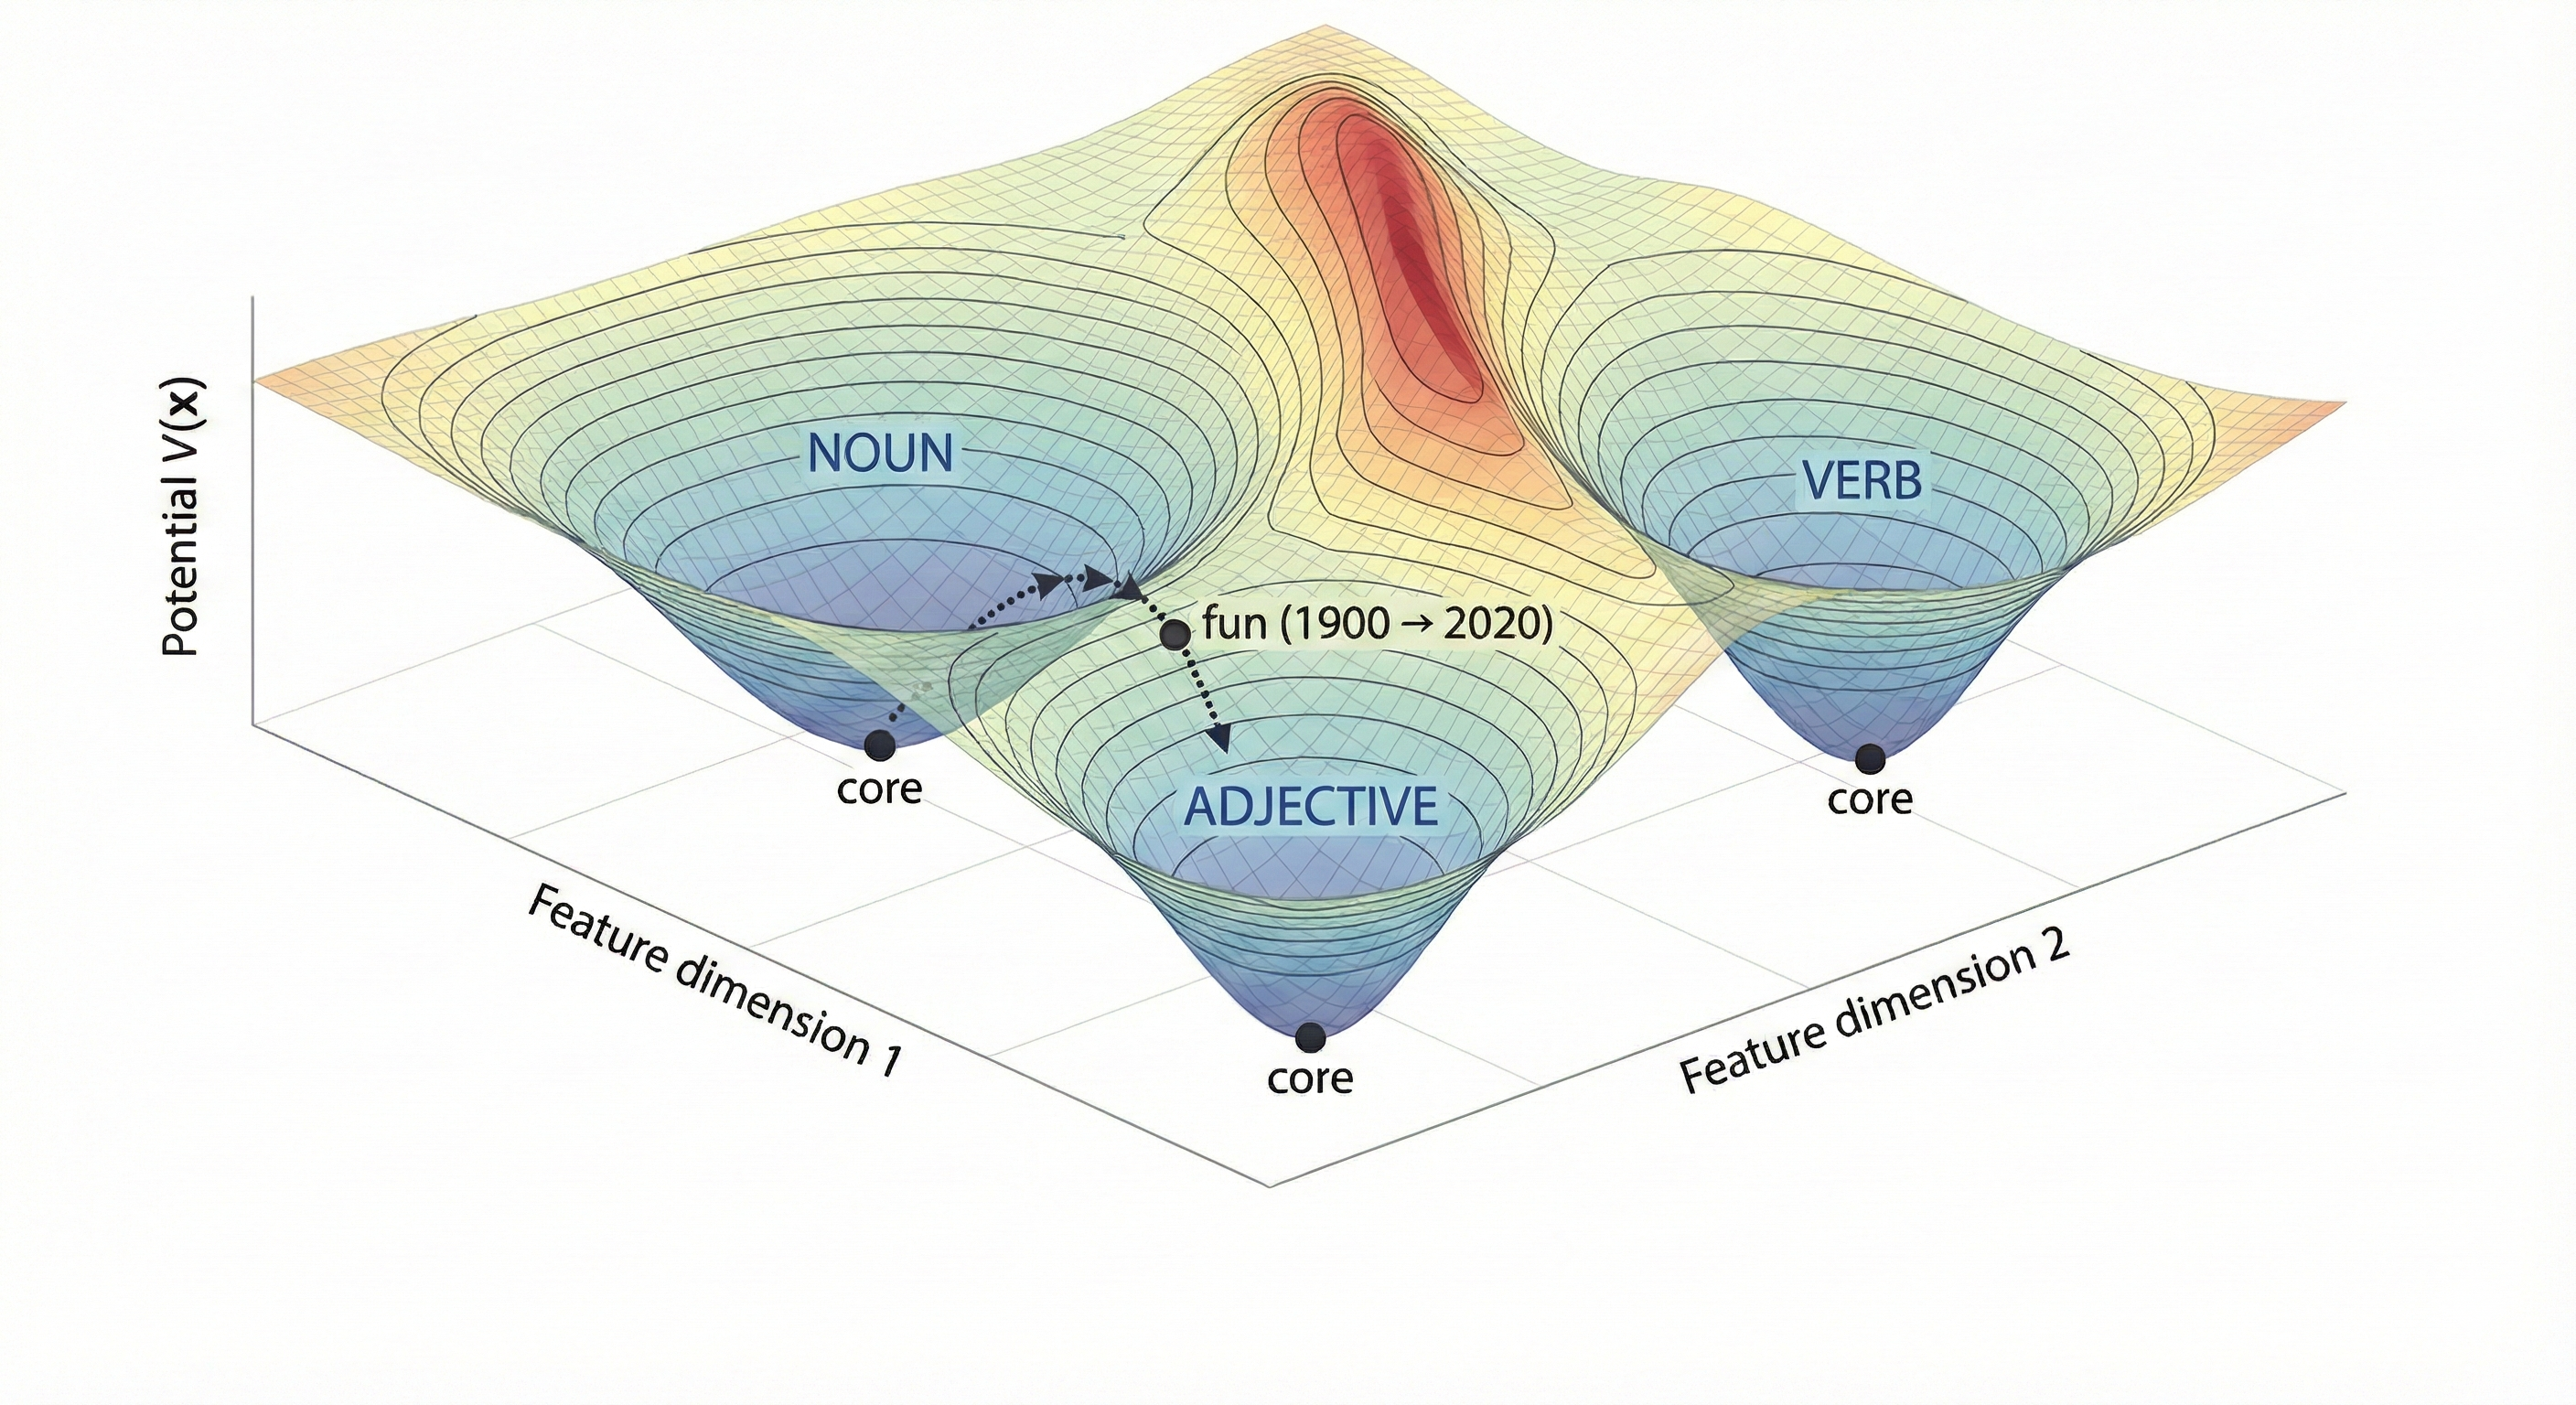
\includegraphics[width=\textwidth]{figures/5.three-basins.png}
\caption{A two-dimensional slice through grammatical feature space, with the potential function $V(\mathbf{x})$ plotted vertically. Category cores correspond to local minima; boundaries to ridges and saddle points. The noun and verb basins are separated by a high ridge (disjoint categories); the noun and adjective basins share a low saddle (porous boundary, overlapping membership possible). The trajectory of \emph{fun} illustrates diachronic movement from deep in the noun basin toward the noun--adjective boundary.}
\label{fig:basin-visualization}
\end{figure}

\paragraph{Basin structure.}
With a metric in hand, the multi-dimensional picture comes into focus. Each category occupies a region in feature space~-- a basin of attraction. Items deep in a basin are stably categorised: small perturbations don't move them out. Items near the boundary are unstable: the same perturbation that would be negligible elsewhere can flip the categorization.

The basins are typically convex. If two items are stably categorised as nouns, items intermediate between them in feature space should generally be too. This is Gärdenfors's criterion for natural categories, and it holds here because the mechanisms maintaining the basin~-- entrenchment, analogy, transmission~-- operate by similarity. Items near the prototype pull their neighbours toward the same categorisation. Apparent non-convexity, where it arises, may indicate that the relevant metric isn't the one assumed, that multiple overlapping basins are being conflated, or that the category has a multi-peaked structure~-- each of these is informative about the mechanisms at work.

The potential-well metaphor captures this: a convex basin corresponds to a single local minimum, and gradient descent from anywhere in the basin leads to the same attractor.

The boundary cases that trouble essentialism~-- \mention{fun}, \mention{near}, \mention{otherwise}~-- are items near basin boundaries. They exhibit properties of multiple categories because they're in the region where tolerance breaks down. Their instability isn't noise; it's evidence about where the boundaries lie.

The categories remain discrete. At any point in feature space, an item is either in category $i$ or not. The boundaries are sharp, located at hyperreal distances that we can't finitely specify. But the \emph{appearance} of gradience arises from epistemic limitations: we observe items at various distances from boundaries, and we can't determine exactly where the boundaries fall. This is \term{real gradience}~-- gradient structure that is genuine evidence about category organisation, not noise to be explained away.

\subsection{Mechanisms and basins}
\label{subsec:5:mechanisms-basins}

The hyperreal model describes the geometry of category boundaries. The HPC framework describes what maintains that geometry. The two are complementary.

Two stories, then. The first is representational: grammatical categories are regions in a feature space, with prototypes at centres and boundaries where similarity to multiple prototypes is balanced. This is the geometry.

The second is causal: the geometry persists because mechanisms~-- acquisition, entrenchment, alignment, transmission, functional pressure~-- exert forces that keep items clustered and boundaries stable. Conceptual-space approaches develop the first story in rich detail \citep{gardenfors2000,gardenfors2014}; HPC frameworks develop the second \citep{boyd1991,boyd1999}.

Both are needed. The geometry tells you what shape the categories have. The mechanisms tell you why they hold that shape.

Rosch's insight that categories have graded internal structure organised around prototypes is preserved~-- but repurposed. What's graded is typicality, not membership. An item is in the category or out; that boundary is sharp. But items inside the category vary in how typical they are, how central to the basin, how far from competing boundaries. HPC retains the gradience while relocating it: not degrees of membership but degrees of stability. A typical noun is one that sits deep in the noun basin, far from competition; an atypical noun sits nearer a boundary, more vulnerable to drift, eruptions, erosion. The mechanisms~-- entrenchment, alignment, transmission~-- are the forces that maintain this structure.

The hyperreal formalisation adds precision about boundaries: sharp but located at unreachable distances, exactly as tolerance intuitions suggest. Prototype theory describes the shape; HPC explains the stability; hyperreals explain the sharpness.

Recall the spinning top from Chapter~\ref{ch:kinds-without-essences}: the stability is dynamic, maintained by active forces rather than static rigidity. Consider what it takes for a basin structure to persist. The boundaries don't maintain themselves. Something has to keep items clustered in their basins; something has to resist drift toward the edges; something has to stabilise the overall configuration. Without such forces, categories would dissolve: items would wander through feature space, edges would shift randomly, the discrete structure would blur into noise.

The homeostatic mechanisms are exactly these stabilising forces. They don't define the boundaries~-- that would be essentialism. They maintain them by exerting pressure on items in feature space.

\textbf{Acquisition} shapes the initial configuration. Children don't learn categories by being told definitions; they induce structure from input. The input reflects the existing basin structure~-- speakers produce items clustered in basins, with boundaries marked by distributional discontinuities. Learners who are sensitive to these patterns acquire the same basin structure, perpetuating it.

\textbf{Entrenchment} deepens the basins. High-frequency items are processed more automatically, stored with greater strength, and more resistant to analogical pressure. They anchor the category, providing stable reference points that other items cluster around. The more entrenched the central members, the steeper the basin walls, the more stable the category.

\textbf{Interactive alignment} maintains consistency across speakers. In conversation, speakers accommodate to each other's usage, converging on shared norms. This creates pressure toward uniformity within a speech community, keeping items in their basins even when individual variation would otherwise push them toward boundaries.

Here is alignment in action. Suppose you say \mention{that was very fun}~-- using the degree modifier that signals adjectival status. Your interlocutor might accommodate, adopting \mention{very fun} in their next turn. Or they might resist, persisting with \mention{a lot of fun}. Either way, the micro-choice shifts local expectations: accommodation reinforces the adjectival pattern; resistance maintains the nominal one. Scale this up across thousands of conversations, and you get the macro-pattern: a word drifting toward or away from a category boundary depending on the balance of accommodation and resistance across the speech community. The mechanism is invisible in any single exchange. The effect accumulates. A two-turn micro-exchange captures the scale: \enquote{That was fun.} \enquote{Yeah, very fun.} Nothing dramatic happens, but a tiny accommodation has occurred~-- and those are the nudges that accumulate into a changed basin.

\textbf{Iterated transmission} filters variation across generations. Not all variants survive transmission; some are easier to learn, easier to produce, easier to understand. The variants that survive tend to be those well inside basins~-- clear exemplars, not boundary cases. Over generations, this filtering effect stabilizes the basin structure.

Consider a thought experiment. You invent a small language~-- twelve signals for twelve meanings~-- and teach it to someone. That person teaches what they learned to a third, who teaches a fourth, and so on. Each link in the chain introduces errors: the learner doesn't quite reproduce what they heard. You might expect the language to degrade into noise. But the opposite happens. Structure emerges.

This isn't speculation. \citet{kirby2008} ran exactly this experiment in the laboratory. Participants learned an artificial language associating nonsense words with coloured shapes, then reproduced it for the next \enquote{generation}. The initial language was random: no pattern connected form to meaning. By generation ten, the language had become compositional~-- word parts systematically encoded colour, shape, and motion. Transmission error dropped from roughly 50\% in the first generation to under 10\%. The key point: no individual designed this structure. As Kirby and colleagues put it, this \enquote{cultural evolution is an `invisible hand' process leading to phenomena that are the result of human action but are not intentional artifacts} \citep[10681]{kirby2008}. The linguistic variants are \term{replicators} in Hull's sense~-- entities that pass copies of themselves through the bottleneck of learning~-- and the communicative episodes are \term{interactors}, where selection pressure applies.\footnote{Hull's replicator/interactor distinction differs from Millikan's copied-kind framework used in Chapter~\ref{ch:kinds-without-essences}. Both capture differential reproduction, but Hull emphasises selection dynamics while Millikan emphasises lineage and proper function. The two frameworks are compatible but not identical.}

Figure~\ref{fig:iterated-learning} shows the pattern. As transmission error decreases (left panel), compositionality increases (right panel). The languages that survive iterated transmission are those easiest to learn~-- and learnable languages, it turns out, are structured languages. The bottleneck of imperfect learning acts as a filter, selecting for systematicity.

\begin{figure}[t]
\centering
\includegraphics[width=0.85\textwidth]{figures/5.iterated-learning.png}
\caption{Structure from transmission. Left: transmission error drops across generations as the language becomes more learnable. Right: compositionality index rises as systematic form--meaning mappings emerge. Data approximated from \citet{kirby2008} and \citet{kirby2015compression}. The pattern shows that iterated cultural transmission, not intentional design, produces linguistic structure.}
\label{fig:iterated-learning}
\end{figure}

The relevance to grammatical categories is direct. If category structure is transmitted imperfectly across generations~-- as it must be, since every child learns anew~-- then the structures that persist are those that survive the transmission bottleneck. Clear exemplars transmit better than boundary cases. Systematic patterns transmit better than exceptions. The basin structure we observe today is the residue of this filtering process, iterated across thousands of generations.

\textbf{Functional pressure} shapes the landscape. Categories exist because they serve functions: nouns package referents for tracking across discourse; verbs encode events and their participants; definiteness signals identifiability. Where functional pressure is strong, basins are deep and boundaries are sharp. Where it weakens, categories erode or restructure.

These mechanisms interact. Functional pressure determines which properties matter; acquisition determines how learners identify them; entrenchment determines which items anchor the category; alignment maintains community-level coherence; transmission filters what persists diachronically. The basin structure at any moment reflects the balance of all these forces.

The hyperreal model tells us what the basin structure looks like: true if irregular boundaries at hyperreal distances, tolerance holding within basins, instability near boundaries. The HPC framework tells us why the structure persists: mechanisms operating across multiple timescales, maintaining the clustering without defining it.

\subsection{Multi-category spaces}
\label{subsec:5:multi-category}

Linguistic categories don't exist in isolation. Nouns compete with verbs; adjectives shade into adverbs; prepositions overlap with both. The basin structure is not a set of independent regions but a tessellation of feature space, with categories abutting each other along shared boundaries. Khalidi calls such overlapping classification schemes \term{crosscutting kinds} and argues they pose no threat to realism: the same entity can be a node in multiple causal networks simultaneously \citep[69--72, 92--97]{khalidi2013}.
This creates additional structure. An item near the noun-verb boundary might be stably a noun (because it's deep in the noun basin) or unstably categorized (because small changes could push it into the verb basin). The same item might be far from the noun-adjective boundary, so its nominal vs.\ adjectival status is never in doubt. Category membership is determinate in multiple dimensions simultaneously, with different degrees of stability in different directions.

Consider the data for \mention{fun}~-- for fun, as it were. In the frequency-of-degree-modification dimension, it has drifted toward adjectives: \mention{very fun} is increasingly acceptable. In the takes-a-determiner dimension, it remains nominal: \mention{the fun we had} is unremarkable. The item sits near the noun-adjective boundary in one dimension, deep in noun territory in another. Its apparent mixed status reflects its location in a multi-dimensional space, not indeterminacy about what categories are.

American historical corpus evidence makes the trajectory visible \citep{davies2010coha}. Degree-modified \mention{fun}~-- \mention{really fun}, \mention{so fun}, \mention{rather fun}, \mention{very fun}~-- is rare through most of the 19th and early 20th centuries but rises sharply from the late 20th century onward: the combined frequency roughly triples between the 1980s and the 2010s. The pattern is consistent with a shift from marginal adjectival-like uses to robust productivity. \mention{Rather fun} shows early isolated footholds (British epistolary usage appears as early as 1827); the American surge comes later. The diagnostics co-move: this is not one fragile string but a bundle of degree environments converging in the same direction.

\begin{figure}[t]
\centering
\begin{tikzpicture}
\begin{axis}[
    width=0.9\textwidth,
    height=4.5cm,
    view={0}{90},
    colorbar horizontal,
    colorbar style={
        at={(0.5,-0.25)},
        anchor=north,
        width=0.6\textwidth,
        height=0.3cm,
        xlabel={Tokens},
        xlabel style={yshift=0.2cm},
        xticklabel style={font=\footnotesize},
    },
    colormap={WhiteBlue}{rgb255(0cm)=(255,255,255); rgb255(0.02cm)=(200,220,255); rgb255(1cm)=(8,48,107)},
    colormap name=WhiteBlue,
    point meta min=0,
    point meta max=55,
    xtick={1,2,3,4,5,6,7,8,9,10,11,12},
    xticklabels={1870,1900,1910,1920,1930,1940,1950,1960,1970,1980,1990,2000s},
    xticklabel style={font=\footnotesize, rotate=45, anchor=east},
    ytick={1,2,3,4},
    yticklabels={\textit{very fun},\textit{so fun},\textit{really fun},\textit{rather fun}},
    yticklabel style={font=\small},
    xlabel={},
    ylabel={},
    enlargelimits=false,
]
% Data matrix: rows = modifiers (bottom to top: very, so, really, rather)
% columns = decades (1870, 1900, 1910, 1920, 1930, 1940, 1950, 1960, 1970, 1980, 1990, 2000s)
% 2000s combines 2000 and 2010 since those are the surge years
\addplot[matrix plot*, mesh/cols=12, point meta=explicit] coordinates {
    % very fun: 1870=1, gaps, 1940=1, 1960=1, 1980=2, 1990=3, 2000s=18
    (1,1) [1]  (2,1) [0]  (3,1) [0]  (4,1) [0]  (5,1) [0]  (6,1) [1]  (7,1) [0]  (8,1) [1]  (9,1) [0]  (10,1) [2]  (11,1) [3]  (12,1) [18]
    % so fun: late surge
    (1,2) [0]  (2,2) [0]  (3,2) [0]  (4,2) [0]  (5,2) [0]  (6,2) [0]  (7,2) [0]  (8,2) [0]  (9,2) [1]  (10,2) [0]  (11,2) [8]  (12,2) [45]
    % really fun: late surge
    (1,3) [0]  (2,3) [0]  (3,3) [0]  (4,3) [0]  (5,3) [0]  (6,3) [1]  (7,3) [2]  (8,3) [3]  (9,3) [9]  (10,3) [6]  (11,3) [25]  (12,3) [52]
    % rather fun: steady early, declines (now row 4 = top)
    (1,4) [0]  (2,4) [3]  (3,4) [5]  (4,4) [2]  (5,4) [7]  (6,4) [5]  (7,4) [7]  (8,4) [7]  (9,4) [3]  (10,4) [1]  (11,4) [2]  (12,4) [2]
};
\end{axis}
\end{tikzpicture}
\caption{Degree-modified \mention{fun} in the Corpus of Historical American English. Darker cells indicate higher frequency. \mention{Rather fun} shows scattered early attestations; \mention{really fun} and \mention{so fun} surge in the 1990s--2000s. The late-century darkening across multiple rows shows convergent adjectivalisation.}
\label{fig:fun-coha}
\end{figure}

\paragraph{Boundary phenomena: operationalising distance.}
The \mention{fun} example shows diachronic drift toward a boundary. But how do we study items that sit \emph{at} a boundary synchronically~-- stably intermediate, not in transition but genuinely in between?

English reciprocals~-- \mention{each other}, \mention{one another}~-- offer a detailed case study \citep{reynolds2025reciprocals}. Standard reference grammars classify them as pronouns, and their distribution supports that much: they head NP-like phrases in the same slots as core pronouns, as verb and preposition complements. But they are non-canonical pronouns. Unlike core personal pronouns, they lack a person/gender/case paradigm and are distributionally defective in the most salient way: they resist ordinary free subject use (cf. \mention{Somebody left} vs. \mention{*Each other left}). 

On the other side, reciprocals are built from determinative material (\mention{each}/\mention{one}) and impose a determinative-like semantic constraint: they are obligatorily anaphoric and require plural antecedents. Yet they are not determiners: they cannot occur in determiner function (*\mention{each other friends} in the intended sense). The point is not to force a verdict from a handful of tests, but to motivate the boundary question: reciprocals sit where the pronoun and determinative profiles exert opposed pulls, making them an ideal probe for how to operationalise stable in-betweenness.

How stable is this in-betweenness? The methodology in \citet{reynolds2025reciprocals} addresses exactly this question by applying three diagnostics:

\begin{enumerate}
\item \textbf{Invariance under analytic perturbation.} Does the boundary position shift when you change the distance metric, the comparison set, or the feature weights? Across multiple correspondence analysis ordinations, Jaccard distances, and specification curves, reciprocals sit midway between pronoun and determinative anchors~-- a stable intermediate, not an artefact of a particular operationalisation.

\item \textbf{Cross-dimensional tension.} Do different feature families pull in different directions? Morphology pulls reciprocals toward determinatives (they lack the case paradigm of core pronouns). Semantics pulls them toward pronouns (they denote referents, not quantities). Syntax and phonology contribute little. The signature of a boundary item is exactly this: opposed pulls from mechanisms that maintain different basins.
\item \textbf{Clear anchors behave cleanly.} Do items unambiguously inside each basin show the expected clustering? Core pronouns like \mention{he} and \mention{herself} sit deep in the pronoun basin; determinatives like \mention{every} and \mention{either} sit deep in the determinative basin. The methodology confirms what intuition expects: the anchors cluster where they should. The interesting finding is that reciprocals don't.
\end{enumerate}

A caveat about statistical significance. Whether the boundary position looks \enquote{statistically significant} depends on which comparison items you choose. Pick one reasonable set and the result is extreme; vary the comparison set and the result wobbles. But the \emph{qualitative} finding~-- reciprocals sit between pronoun and determinative anchors~-- is stable across all choices. Under an HPC reading, this is exactly what genuine boundaries should look like: the diagnosis persists, but decisive p-values elude us because the item really is intermediate.

This operationalises the chapter's theoretical picture. \enquote{Distance to boundary} is not metaphorical; it can be measured. \enquote{Stability of ambiguity} is not vague intuition; it is invariance under analytic perturbation~-- the in-betweenness persists when you change your measurement instrument. Reciprocals sit in the overlap region of Figure~\ref{fig:disjoint-overlap}, not because the analysis went wrong but because the basin structure itself has overlap.

The same analysis applies to the existential debates about feature systems raised in §\ref{sec:3:lexeme-obsession}. Is \textsc{gender} a natural kind, or is it reducible to \textsc{number}? The question becomes: do gender and number occupy distinct basins maintained by distinct mechanisms, or is gender a sub-region of a larger number basin, maintained by the same mechanisms at a finer grain?

If the mechanisms maintaining gender systems~-- agreement patterns, acquisition pathways, functional pressures toward nominal classification~-- are distinct from those maintaining number systems, then gender is a genuine natural kind: a separate basin in the space of grammatical features. If the mechanisms overlap substantially~-- if gender turns out to be number's machinery for individuation, as some theorists have argued~-- then the basins merge, and \textsc{gender} as a cross-linguistic category dissolves into \textsc{number}.

This is an empirical question, not a definitional one. The hyperreal model tells us what to look for: distinct basins with true if irregular boundaries and scale-dependent tolerance. The HPC framework tells us how to investigate: identify the mechanisms, trace their operation, determine whether they cluster distinct properties or the same properties at different scales.

Consider the Shilluk number system introduced in §\ref{sec:3:lexeme-obsession}. English marks number with a suffix: \mention{cat}, \mention{cats}. Shilluk marks it through stem-internal changes in tone, vowel length, and voice quality~-- a singular/plural pair might differ only in whether the vowel is short, long, or overlong, or in whether the tone is Low or Fall. The exponence is lexicalised: each pair must be learned; no productive rule derives one from the other.

What does the HPC + hyperreal view say about this? Both English and Shilluk number systems occupy basins in a feature space whose dimensions include obligatoriness (number must be specified), agreement scope (specifier, verb, other constituents), and semantic function (individuation of entities). The exponence dimension~-- where English is affixal and Shilluk is fusional/suprasegmental~-- places them in different regions of morphophonological space but the same region of morphosyntactic and semantic space. They're in overlapping basins, not identical ones~-- independent systems shaped by similar pressures, not one system shared across languages.

The mechanisms maintaining the two systems are partially shared (acquisition of obligatory contrast, iterated transmission of the singular/non-singular distinction) and partially distinct (rule-based productivity in English, lexical storage in Shilluk). The prediction is that where the mechanisms align~-- the functional pressure to distinguish singular from plural~-- the categories should pattern similarly across languages. Where they diverge~-- the phonological substance of the exponence~-- we should expect variation. That's exactly what we find. The basin boundary for \textsc{number} is sharp in both languages (a noun is singular or plural, not in between), but the basin's location in the full feature space differs, because different mechanisms weight different dimensions. The same analysis extends to noun-class systems like Swahili's, to Mandarin classifiers, to German gender. Wherever there's grammatical categorisation, there should be basin structure maintained by mechanisms.

A question arises: is the cross-linguistic similarity \emph{convergence} or \emph{homology}? In biology, convergence means similar phenotypes arising independently (the wings of bats and birds), while homology means similarity inherited from a common ancestor (the forelimbs of all mammals). For \textsc{number}, the answer is probably convergence: the functional pressure to distinguish singular from plural exists in any language with nominal reference, and different languages have evolved different morphological solutions. The mechanisms overlap not because of common ancestry but because of common function. For \textsc{noun} and \textsc{verb}, the answer might be different: if these categories reflect universal constraints on predication and reference, they may be homologous~-- inherited from whatever cognitive architecture makes human language possible. The framework should distinguish these cases, and the mechanistic analysis provides the tools: shared mechanisms suggest homology; parallel mechanisms suggest convergence.

If the HPC analysis just confirms that English number and Shilluk number are both \textsc{number}, have we learned anything? Yes: the framework explains \emph{why} they deserve the same label~-- not definitional fiat, but overlapping mechanisms maintaining overlapping basins. And it makes predictions: if we found a putative \enquote{number} category maintained by entirely different mechanisms with no overlap in the functional dimension, the framework would say it's not the same kind~-- same label, different basin.

\section{Empirical consequences}
\label{sec:5:empirical-consequences}

\subsection{Gradient judgments, discrete categories}
\label{subsec:5:gradient-discrete}

The discreteness problem has a close cousin: the gradient-judgment problem. Speakers' acceptability judgments are notoriously gradient. Asked to rate sentences on a 1--7 scale, they distribute across the range, with clear acceptability at the extremes and uncertainty in the middle. If categories are discrete, why are judgments gradient?

The hyperreal framework suggests an answer. Distinguish the category from its measurement, the ontology from its epistemology.

\textbf{Grammaticality}~-- the property of conforming to the grammar~-- is discrete. A sentence either satisfies the constraints or it doesn't. The boundary between grammatical and ungrammatical is sharp, located at a hyperreal threshold in some underlying dimension (perhaps accumulated constraint violation, or distance from prototype, or processing cost).

\textbf{Acceptability}~-- the measured response in judgment tasks~-- reflects grammaticality filtered through noise. Processing difficulty, frequency effects, task demands, individual variation, and measurement error all intervene between the discrete category and the gradient response.

One reason this distinction is so easy to lose sight of is that the phenomenology is asymmetric. When a sentence is well-formed, nothing in particular announces itself: processing just runs. The felt data are mostly negative~-- the \enquote{catch} of a violation, the extra effort, the moment of repair. There is, in that sense, no positive feeling of grammaticality, just as there is no feeling of having sufficient oxygen; the experiences that demand attention are the absences. This is why boundary detection is cognitively natural: violations have a signature, conformity is typically silent.

A second reason is methodological. Temperature is not something you see; it is a theoretical magnitude inferred from what thermometers do. Likewise grammaticality is a latent property that we access only through instruments~-- judgments, reaction times, eye movements, priming, production choices~-- each of which can misread the target in both directions, yielding false comfort (illusory well-formedness) or false alarm (grammatical but degraded). The point is clearest in \emph{satiation} effects: repeated exposure can raise acceptability for initially degraded strings, even though it is implausible that the grammar itself has been rewritten over the course of a short experimental session. Satiation is therefore not a nuisance; it is direct evidence that the mapping from grammaticality to felt acceptability is plastic, and that we should not identify the construct with any one measurement channel.

Not all of these factors work the same way. Random fluctuations~-- trial-to-trial variation in attention, incidental processing load, measurement noise~-- blur the signal without shifting it. But frequency effects and task demands can systematically shift the mapping from grammaticality to acceptability. A borderline construction may be judged more acceptable if it's high-frequency than if it's low-frequency, even when both are equally grammatical. Instructions emphasising naturalness may locate the boundary differently than instructions emphasising correctness. These are biases, not noise. The two-layer model accommodates them: different contexts may activate different effective basin configurations, shifting where tolerance breaks down.

This predicts:
\begin{itemize}
\item Clear cases cluster at scale extremes (1s and 7s), because items deep in the grammatical or ungrammatical basin are stably categorized and noise doesn't flip them.
\item Borderline cases distribute across the middle, because items near the boundary are sensitive to noise~-- small processing fluctuations can shift judgments in either direction.
\item The gradient spread is widest near the boundary, because that's where the signal-to-noise ratio is lowest (see Figures~\ref{fig:two-layer-model} and~\ref{fig:judgment-variance}).
\end{itemize}

This is a testable prediction. If the two-layer model is right, items independently rated as near category boundaries should show higher variance in acceptability judgments than items rated as central. The prediction isn't that boundary items get middling ratings~-- that's compatible with gradient grammaticality~-- but that their ratings should be more variable across trials and subjects. The pattern should show up as a hyperbolic relationship between distance-to-boundary and judgment variance. Existing work on gradient acceptability already points in this direction: \citet{sprouse2013} found that judgment variability correlates with distance from prototypical (un)grammaticality, and \citet{dabrowska2010} showed systematic individual differences in judgments of complex constructions~-- exactly what you'd expect if different speakers have slightly different basin structures.

This last point deserves emphasis. The basin structure isn't uniform across speakers. Speakers with different input histories~-- more or less exposure to written registers, different dialectal backgrounds, varying levels of literacy~-- will have basins with different shapes and different boundary locations. The hyperreal model accommodates this naturally: each speaker's grammar is a different model, with a different boundary index $K$. What varies across speakers isn't just noise; it's the underlying geometry. The framework predicts that variability in judgments should be highest for constructions that fall near the boundary \emph{for most speakers}~-- and that speakers who agree on central cases may nonetheless diverge on peripheral ones, because their boundaries are located at different hyperreal indices.

\begin{figure}[t]
\centering
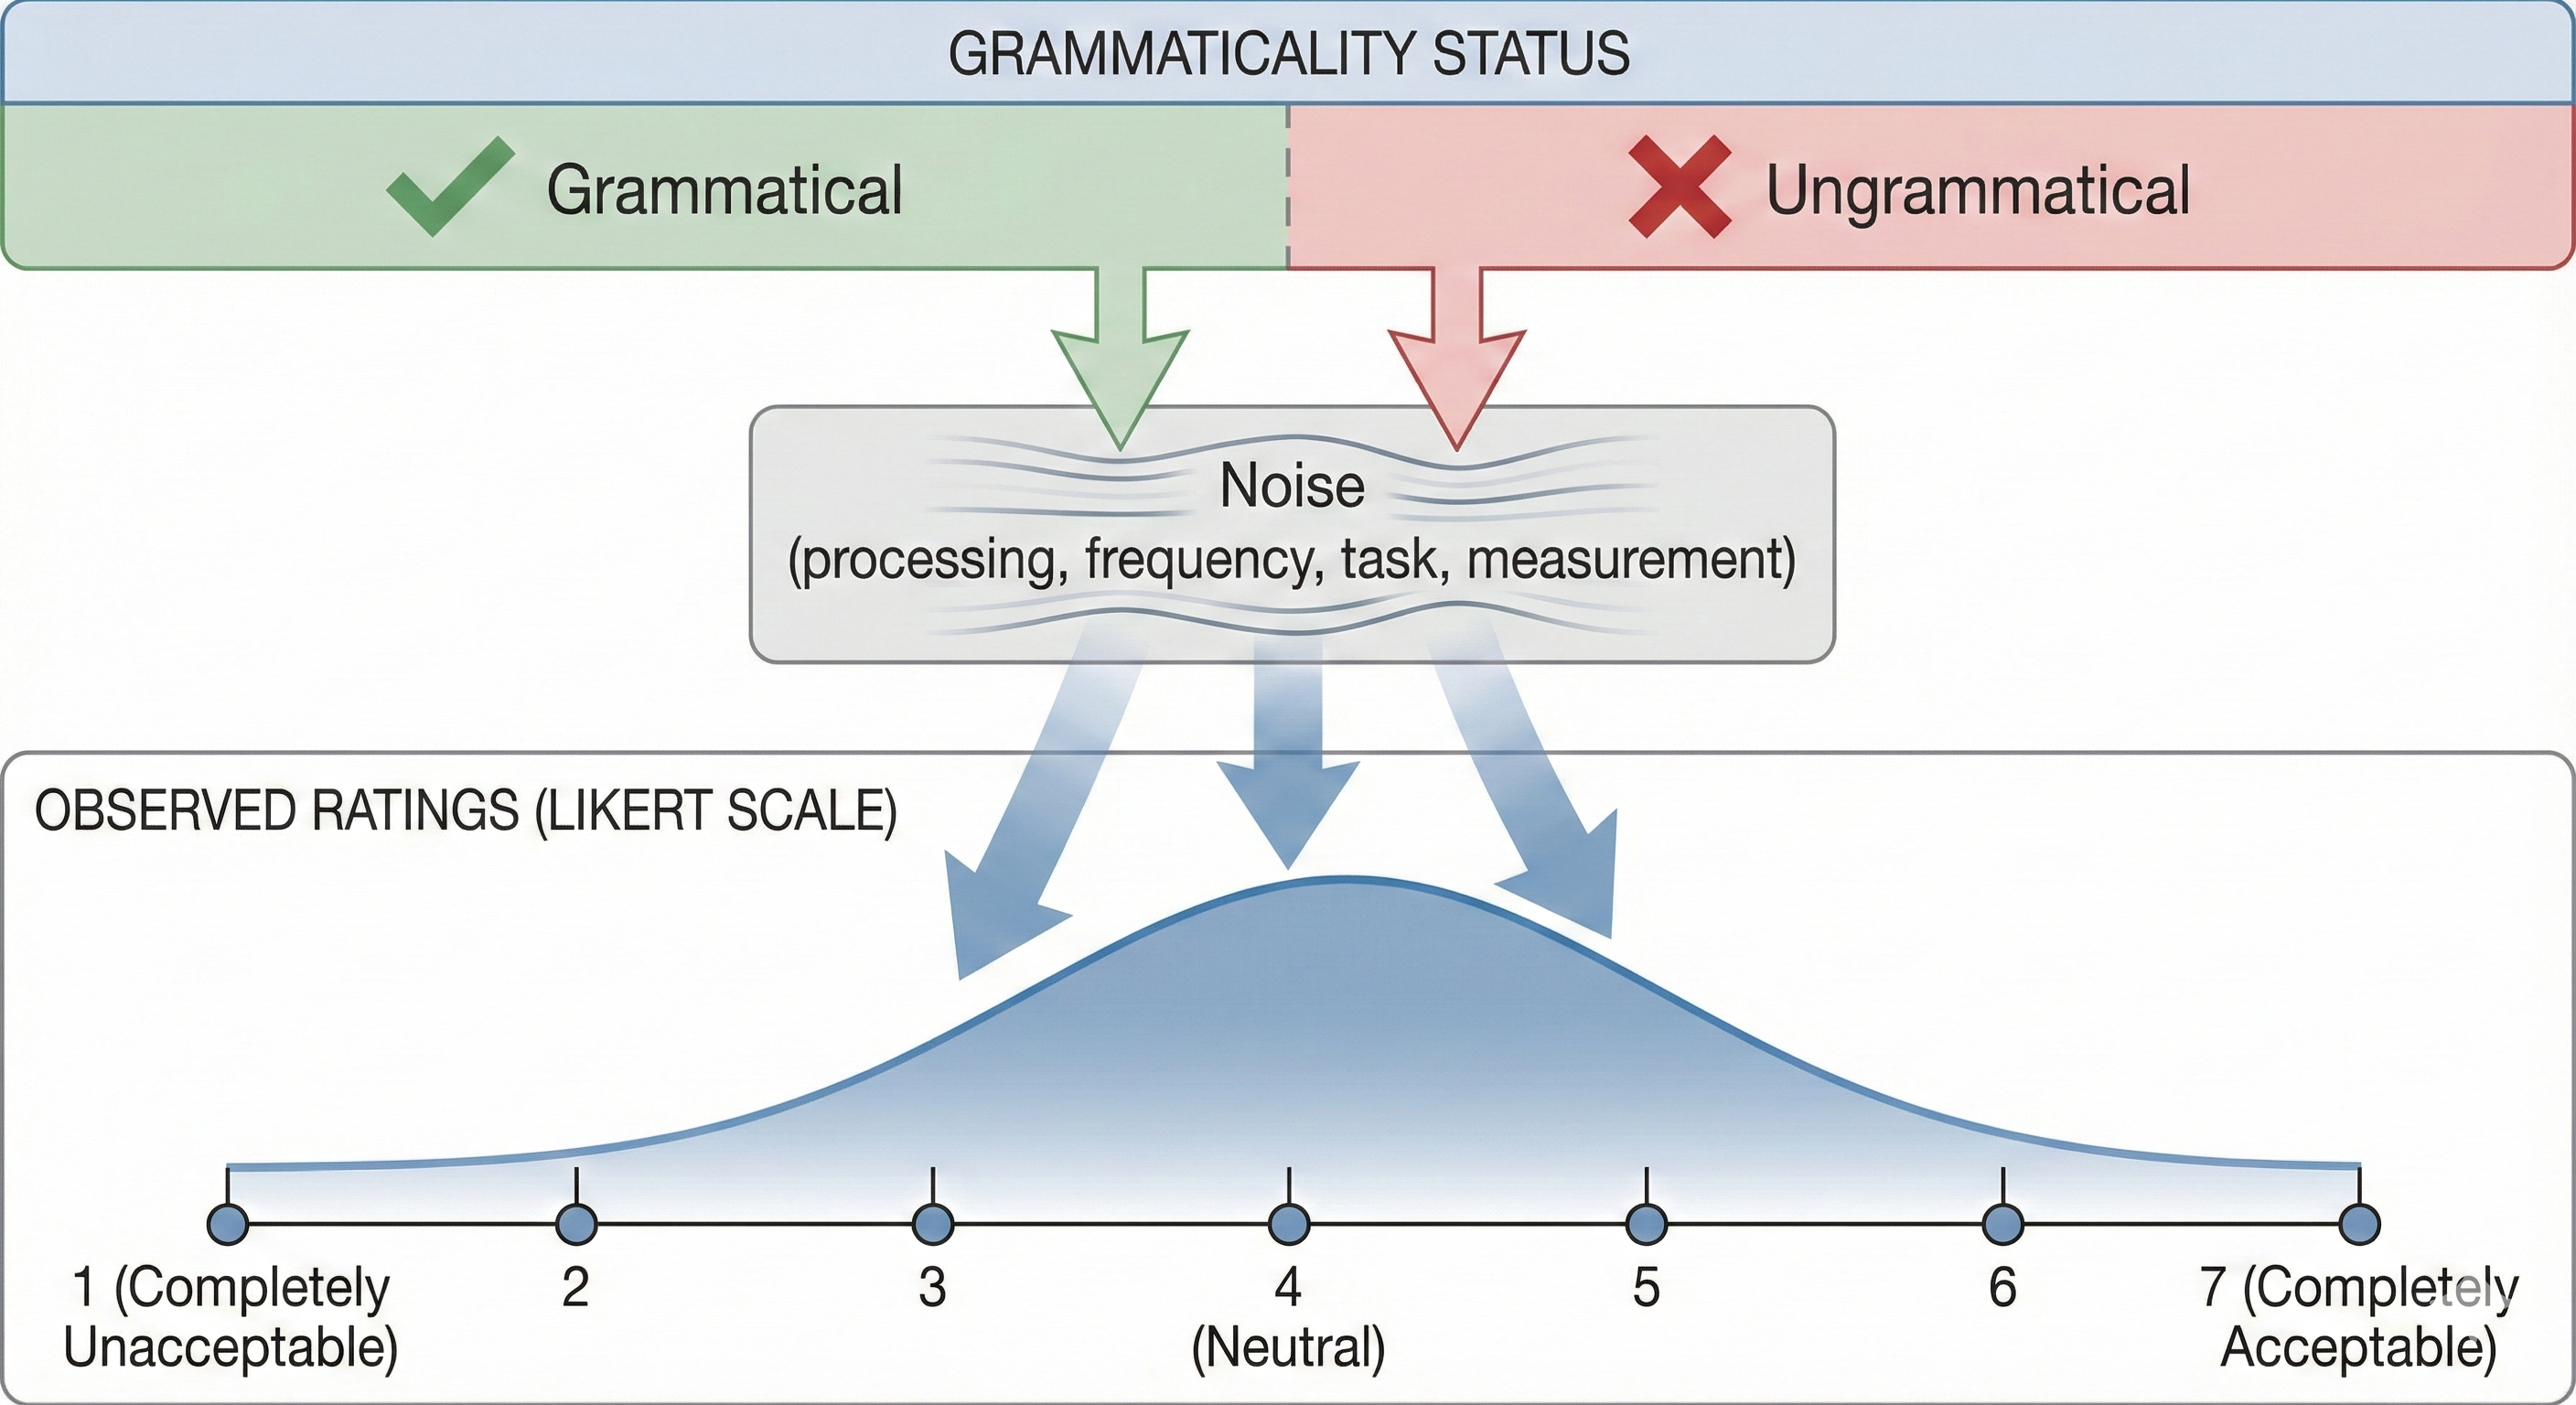
\includegraphics[width=0.85\textwidth]{figures/5.two-layer-grammaticality.png}
\caption{The two-layer model. Discrete grammaticality (binary: grammatical or ungrammatical) is filtered through processing and measurement noise to produce gradient acceptability judgments. Items deep in basins produce stable judgments at scale extremes; items near boundaries produce variable judgments distributed across the middle of the scale.}
\label{fig:two-layer-model}
\end{figure}

\begin{figure}[t]
\centering
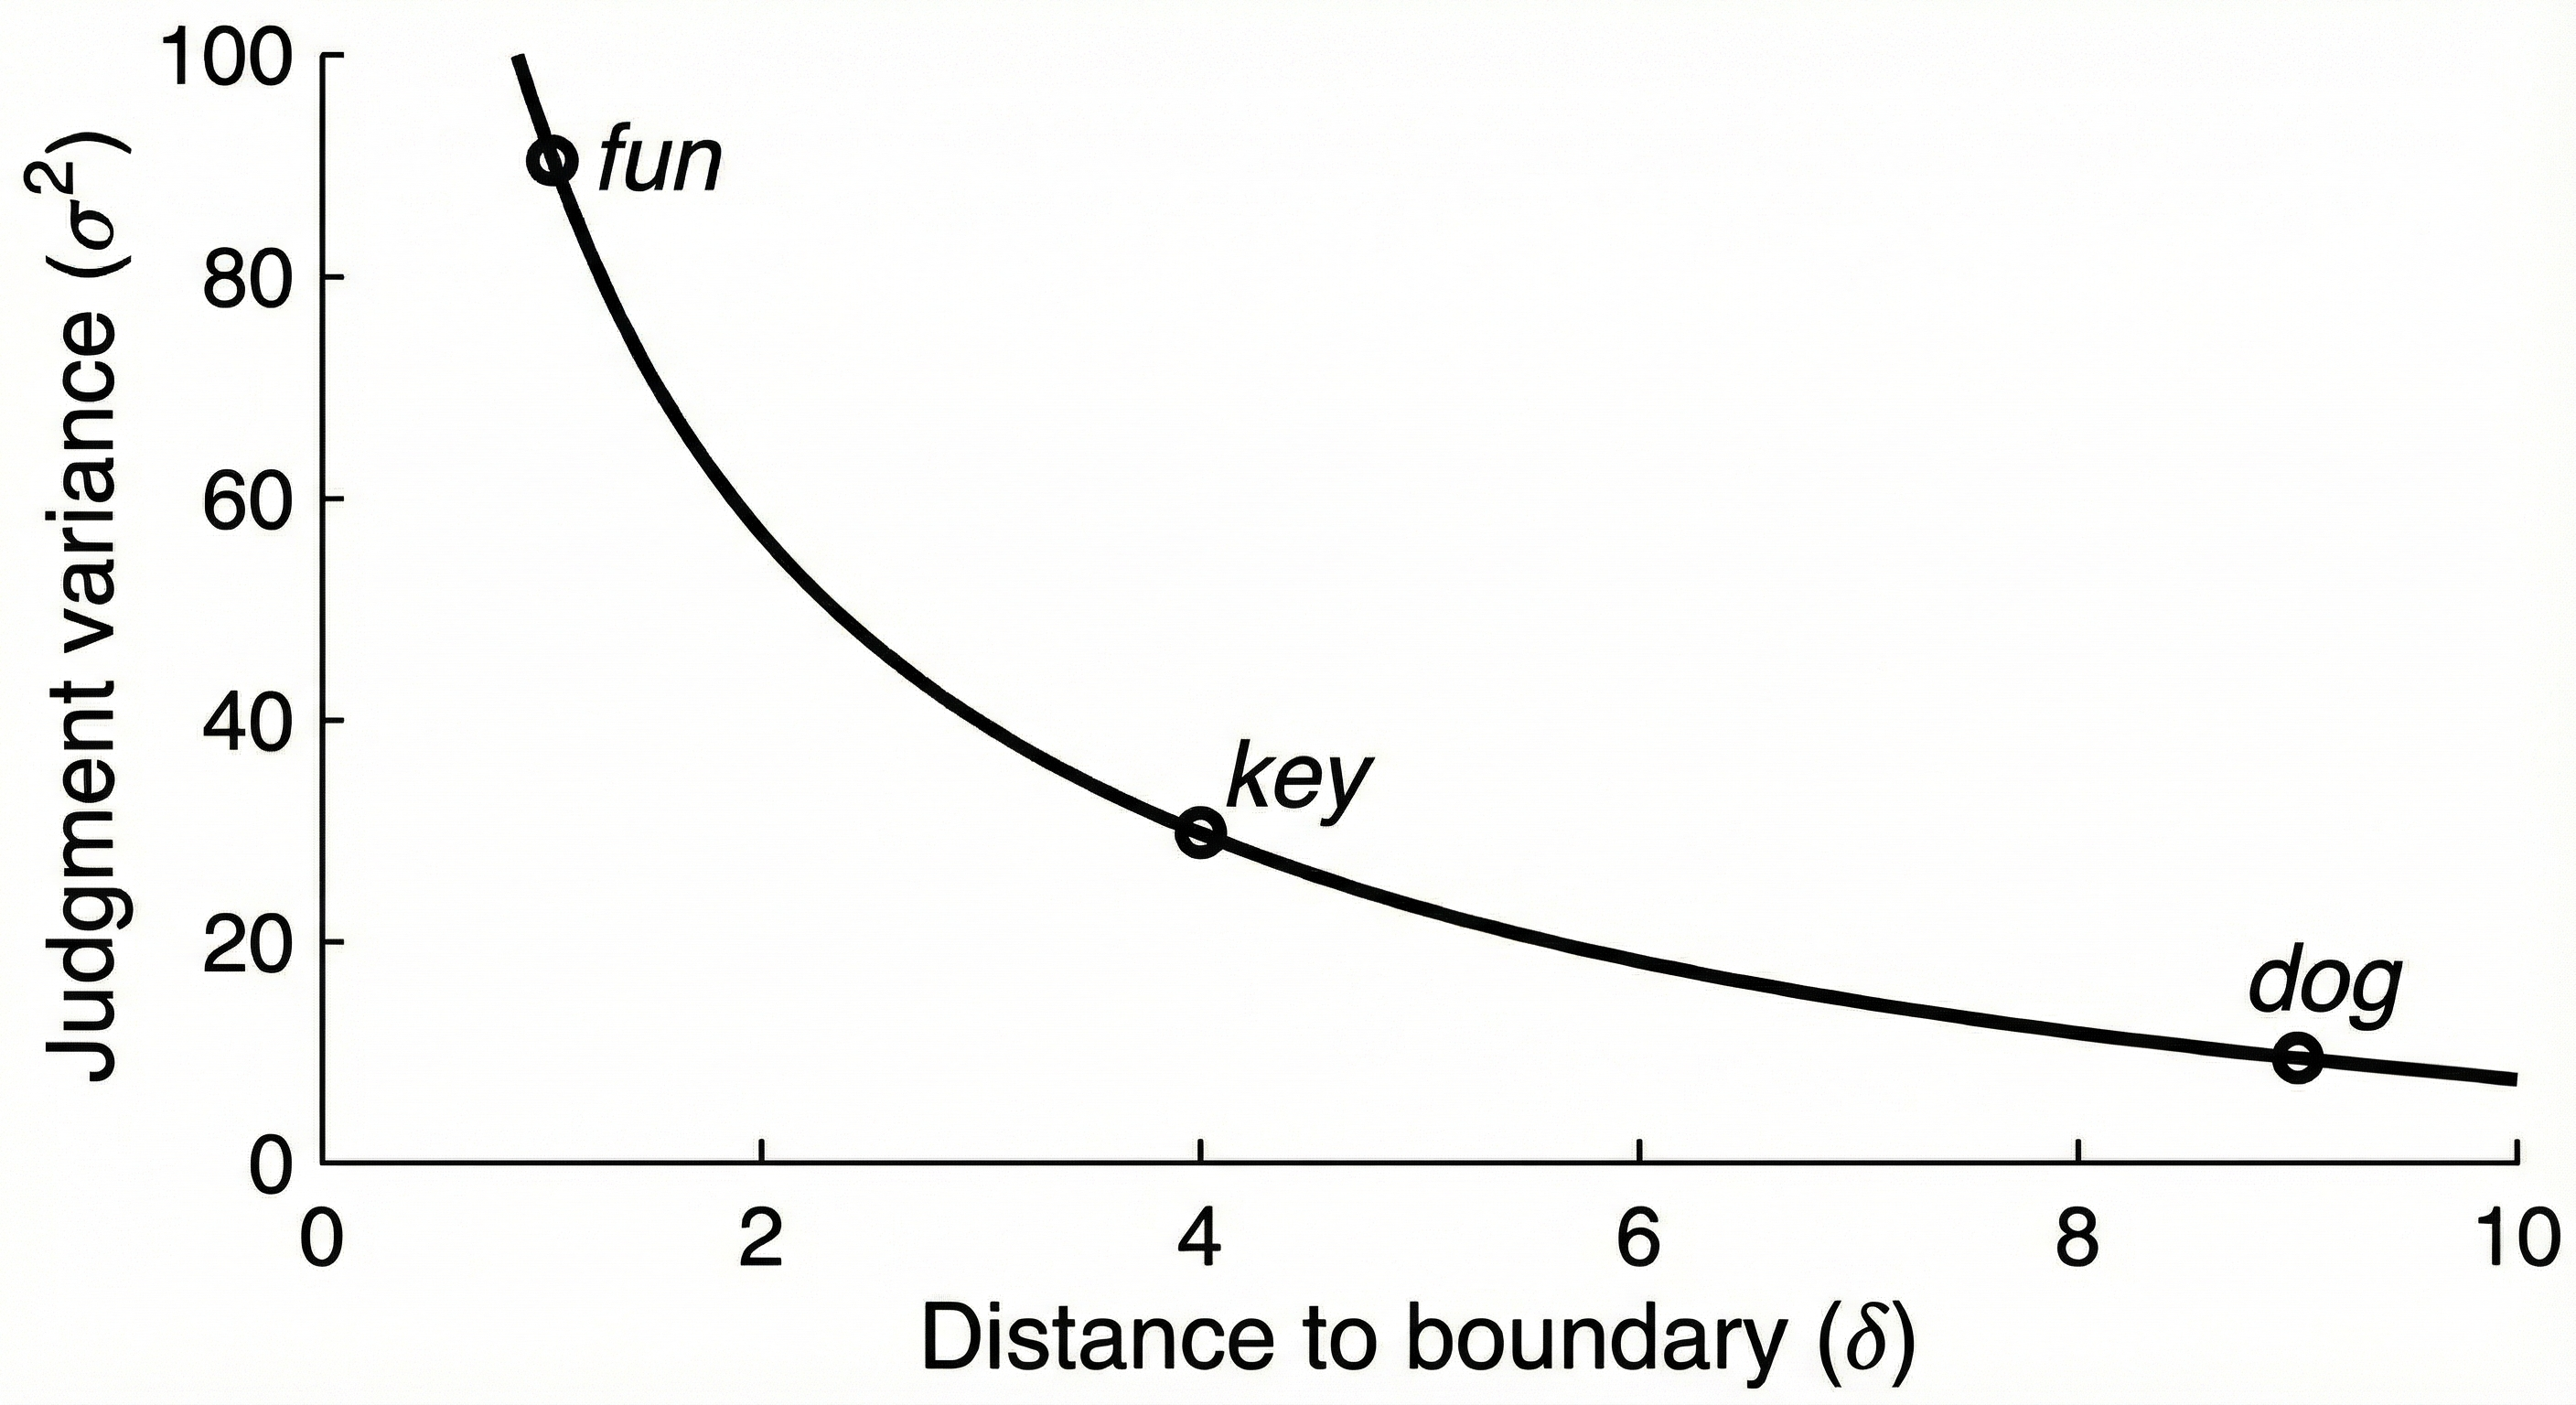
\includegraphics[width=0.85\textwidth]{figures/5.judgment-variance.png}
\caption{Predicted relationship between distance to category boundary and acceptability judgment variance. Items deep in basins (e.g., \mention{dog}) show stable judgments with low variance; items near boundaries (e.g., \mention{near}) show high variability. The hyperbolic relationship reflects the signal-to-noise ratio degrading as items approach the boundary.}
\label{fig:judgment-variance}
\end{figure}

This is not a new observation~-- the distinction between competence and performance has been with us since Chomsky. But the hyperreal framework adds precision. The boundary is not merely \enquote{somewhere in the grammar}; it's located at a specific (if unspecifiable) hyperreal threshold. The gradience is not merely \enquote{performance noise}; it's the predictable consequence of epistemic limitations near a sharp boundary.

Chapter~\ref{ch:grammaticality-itself} develops this picture fully, arguing that grammaticality itself is a homeostatic property cluster~-- a category maintained by mechanisms, with a sharp boundary at hyperreal distance. For now, the point is that gradient judgments and discrete categories are compatible. The discreteness is in the structure; the gradience is in our access to it.

\subsection{Dual membership}
\label{subsec:5:dual-membership}

One puzzle remains. If categories are discrete~-- if at every point in feature space an item is either in or out~-- how can there be genuine dual membership? How can \mention{near} be both a preposition and an adjective, not contextually selected, not in transition, but stably both? English is comfortable with a kind of dual citizenship here: items like \mention{near} can hold both passports without being in transit.

The answer is that discreteness holds predicate-by-predicate, not across predicates. The predicates \textit{is a preposition} and \textit{is an adjective} are each bivalent: at any point, each is either true or false. But they're not mutually exclusive. The basins can overlap.

This follows naturally from the HPC framework. Categories are maintained by mechanisms, not defined by partition. The mechanisms maintaining prepositionhood~-- patterns of complementation, head-of-PP status, lack of degree modification~-- are partially independent of those maintaining adjectivehood~-- gradability, predicative use, comparative morphology. An item can fall within the tolerance threshold for both, satisfying the clustering criteria for each.

Where the mechanisms align, the basins are disjoint: nouns and verbs occupy separate regions because the mechanisms that maintain them pull in different directions (Figure~\ref{fig:disjoint-overlap}, left). Where the mechanisms cross, the basins overlap: adjectives and prepositions share enough properties~-- predicative function, modification of nominals~-- that some items cluster with both (Figure~\ref{fig:disjoint-overlap}, right).

The regions of overlap are not arbitrary. They're located where the property clusters themselves overlap~-- where an item can satisfy the tolerance criteria for both categories simultaneously. These are exactly the cases that trouble essentialism: items that have \enquote{mixed} status because they satisfy criteria for multiple categories. On the HPC + hyperreal view, mixed status is not indeterminacy but dual location: the item is in two basins at once, stably, because the mechanisms that maintain each basin both apply.

The reciprocals case from §\ref{subsec:5:multi-category} exemplifies this cleanly. Morphology maintains the determinative basin; semantics maintains the pronoun basin. Reciprocals satisfy both. The mixture weights from the blend model~-- 0.534 pronoun-like for \mention{each other}, 0.487 for \mention{one another}~-- are not noise or measurement error. They are the empirical signature of genuine dual location: stable membership in overlapping basins, maintained by partially independent mechanisms.

\begin{figure}[t]
\centering
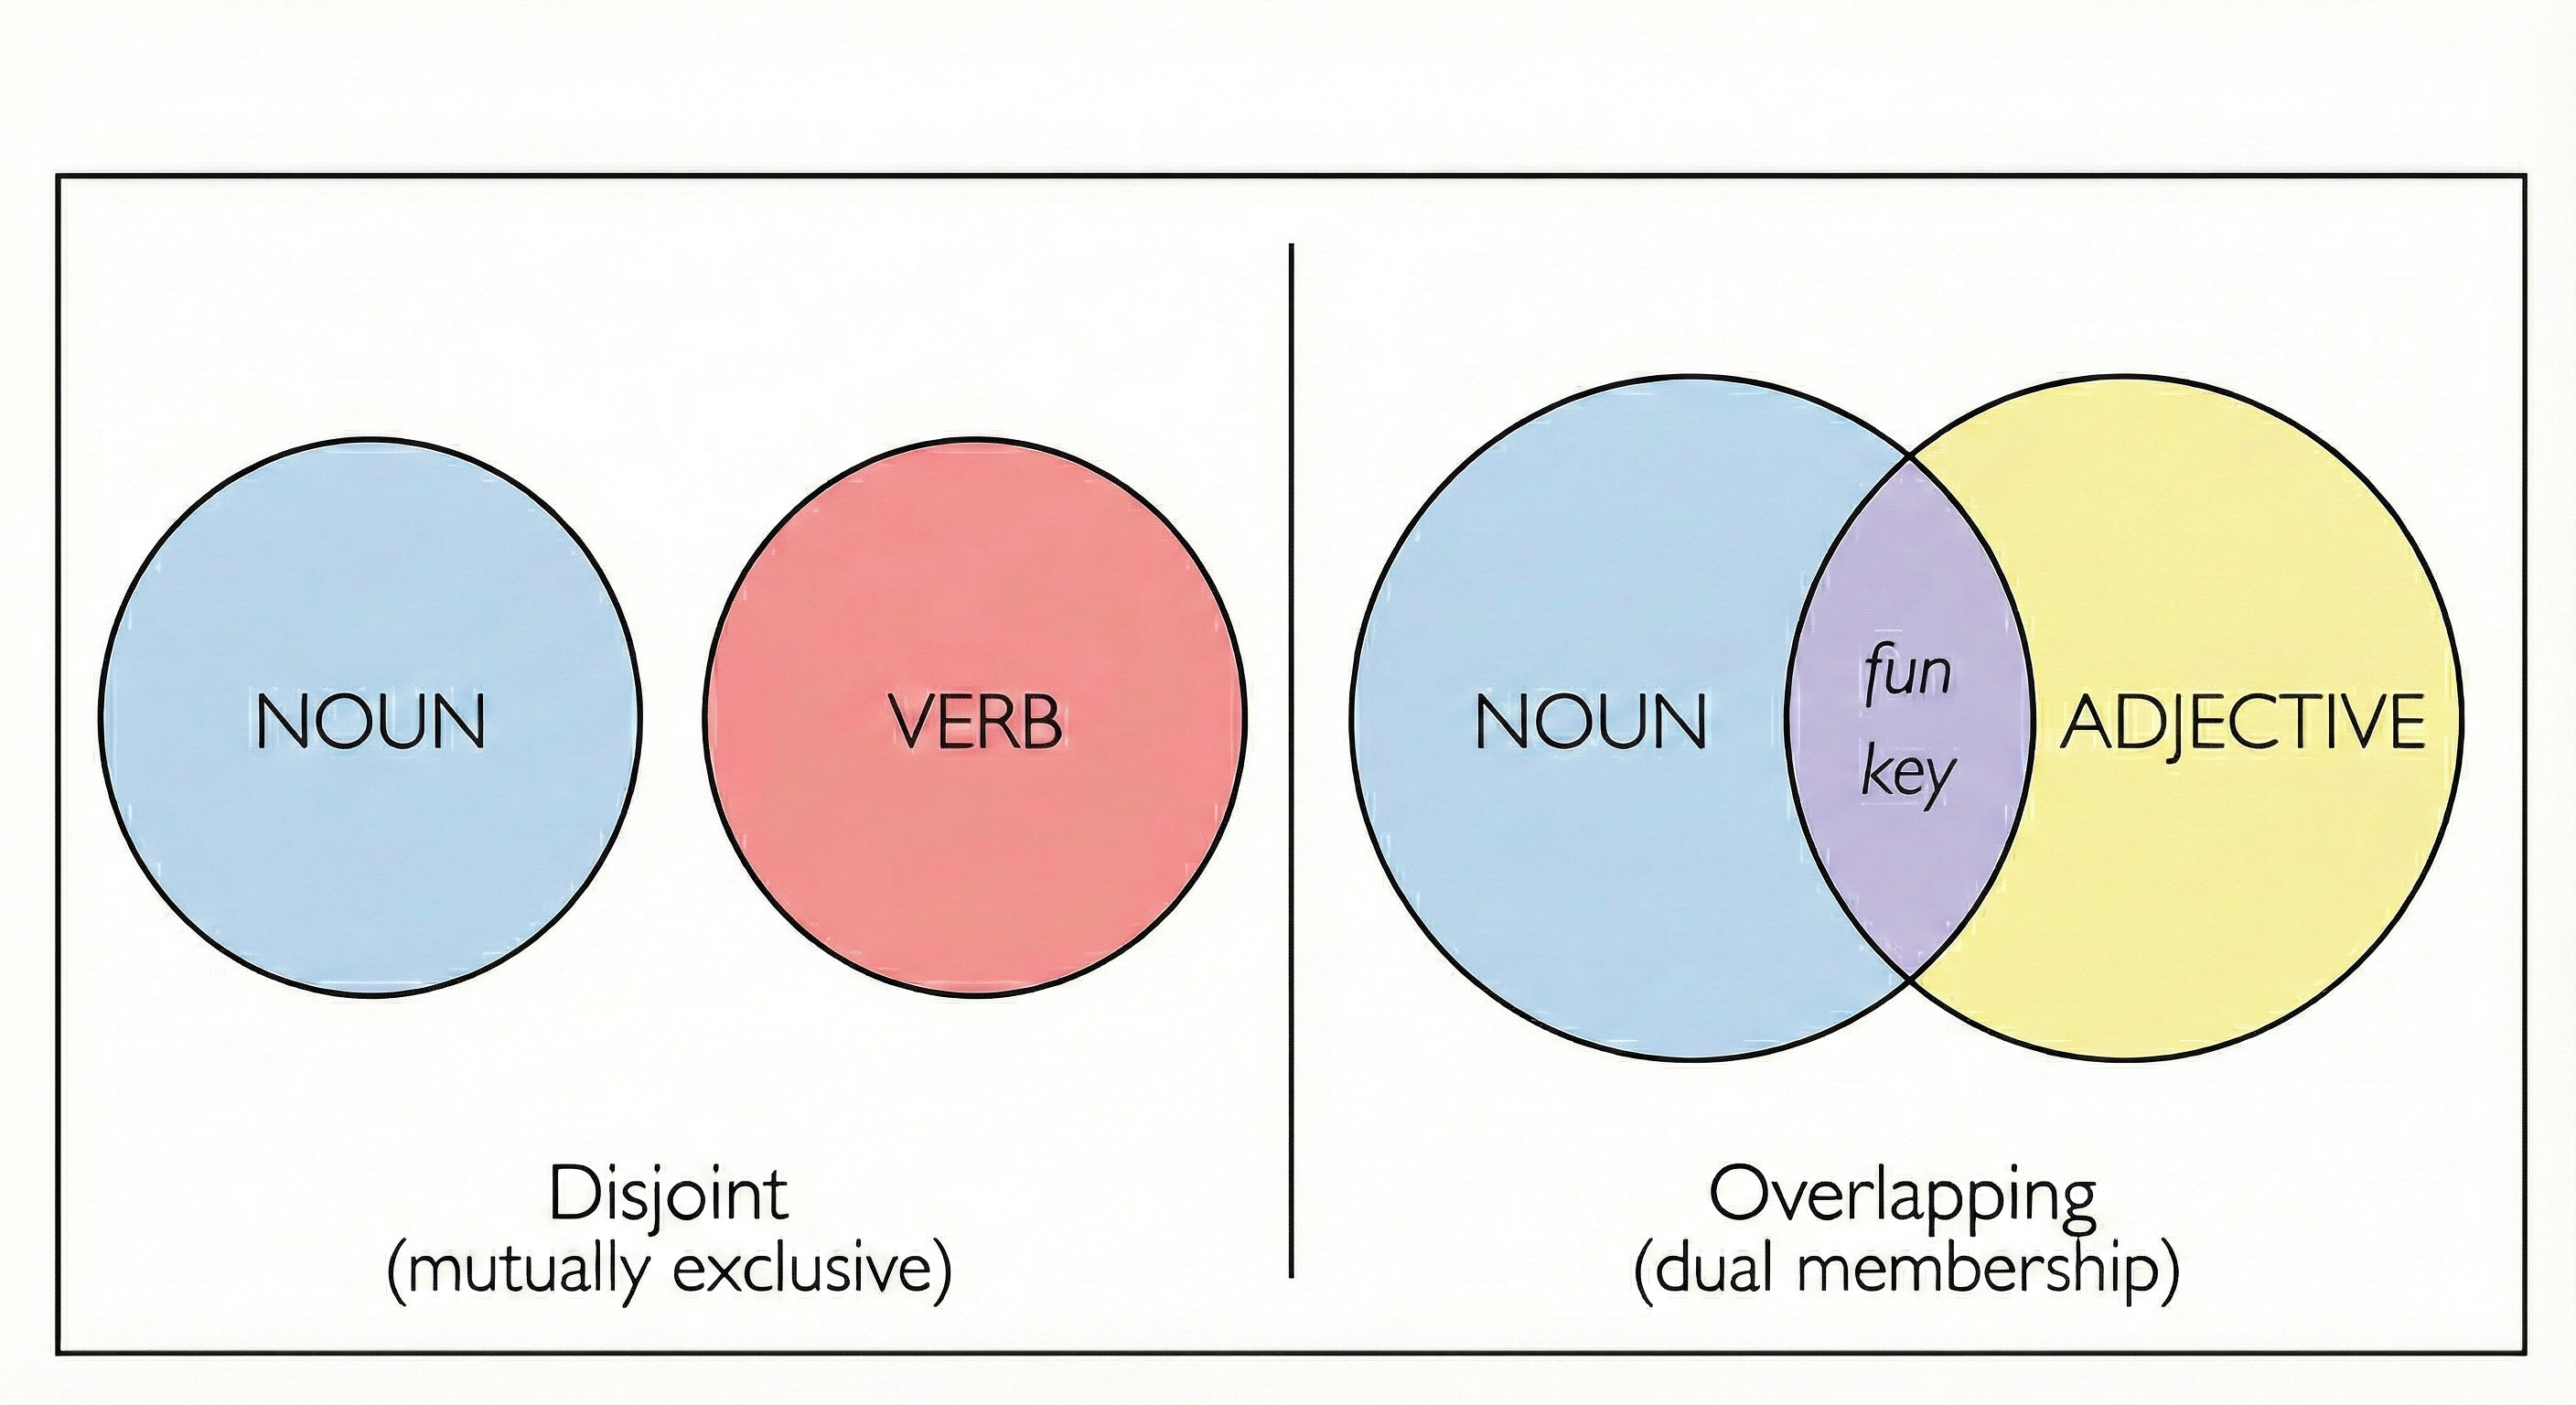
\includegraphics[width=0.85\textwidth]{figures/5.disjoint-overlap.png}
\caption{Disjoint vs.\ overlapping category basins. Left: noun--verb mechanisms pull in opposite directions, creating mutual exclusivity. Right: noun--adjective mechanisms are partially independent, permitting overlap. Items like \mention{fun} and \mention{near} occupy the overlap region, satisfying the clustering criteria for both categories simultaneously.}
\label{fig:disjoint-overlap}
\end{figure}

\subsection{Summary: discreteness without essence}
\label{subsec:5:discreteness-summary}

The discreteness problem asked: if underlying properties are continuous, how do discrete categories emerge?

The answer combines two components:

\textbf{Structure (hyperreal model):} Discrete boundaries arise from scale-dependent tolerance. Changes that are negligible at the current scale preserve categorization; changes that are appreciable can flip it. The boundary is sharp, located at a hyperreal threshold, epistemically inaccessible but structurally determinate. Dynamic discreteness is like a snow-covered streetcar right-of-way: the snowfall is continuous, but the rails impose two stubbornly sharp tracks that exist only because of the system underneath them.

\textbf{Maintenance (HPC framework):} The basin structure persists because mechanisms~-- acquisition, entrenchment, alignment, transmission, functional pressure~-- hold properties together. Without these mechanisms, categories would dissolve. With them, the clustering is stable even though boundaries are fuzzy at the edges.

Together, these explain how categories can be:
\begin{itemize}
\item \textbf{Real}: maintained by causal mechanisms, not merely stipulated.
\item \textbf{Discrete}: with sharp boundaries, not gradient membership.
\item \textbf{Fuzzy at the edges}: because tolerance fails near boundaries, producing instability and apparent gradience.
\item \textbf{Stable}: because mechanisms maintain the basin structure across time.
\item \textbf{Capable of change}: because mechanisms can shift, basins can migrate, boundaries can move.
\end{itemize}

This is what the essentialist wanted~-- real structure, sharp boundaries, determinacy~-- without what the essentialist thought was required: definitions, necessary and sufficient conditions, essences. The categories are real because they're maintained, not because they're defined. The boundaries are sharp because tolerance is scale-dependent, not because some property is binary. The determinacy is causal-structural, not definitional.

The nominalist was right that essences don't exist. The nominalist was wrong to conclude that determinacy fails. The HPC framework, formalised via hyperreal tolerance, shows how to have both: natural kinds without essences, discrete categories from continuous substrates, sharp boundaries that we can't quite see. Dynamic discreteness and real gradience~-- the chapter's twin themes~-- turn out to be two sides of one insight.

\chapter{Projectibility and the good bet}
\label{ch:projectibility}

% SLOGAN: Categories earn their keep by supporting induction.
% Sticky sentence: "The mechanism projects even though the category, as traditionally defined, doesn't."
% See notes/book-slogans.md for the book-wide slogan strategy.

\epigraph{If there are not [pedicabs], Mr Tagomi thought, I would be well advised to retire to secluded place and kill myself.}{Philip K. Dick, \textit{The Man in the High Castle}}

The previous chapter established that grammatical categories are real~-- maintained by mechanisms, not defined by essences. This chapter asks what we get in return. If categories aren't defined, why should learning about one instance tell us anything about others?

The answer is \term{projectibility}: the ability of a category to support inductive inference. You learn that \mention{dog} is a noun~-- it takes determinatives, pluralises, functions as an argument. From this, you infer that unfamiliar nouns will behave similarly. The inference isn't guaranteed; \mention{sheep} doesn't pluralise the usual way. But it's reliable enough to be useful. That's projectibility: learning from instances and projecting to the category.

The essentialist has a ready explanation. Categories support induction because they have definitions. If something satisfies the definition, it has the defining properties; those properties are what you project. Simple.

The trouble is that the explanation requires definitions we don't have. Chapter~\ref{ch:essentialism} showed that no list of necessary and sufficient conditions distinguishes nouns from non-nouns, verbs from non-verbs. So where does projectibility come from?

The HPC answer: mechanisms. Categories support induction not because they're defined but because they're mechanistically grounded. The mechanisms that maintain the category also explain why its members resemble each other. Learning about one member tells you about others because the same mechanisms shaped both.

The pattern shows up even in computational models trained without linguistic theory. \citet{decarlo2023} probed language models on negative polarity items---words like \mention{ever}, \mention{squat}, and \mention{anymore} that require licensing contexts like negation or questions. The category \term{NPI} looks uniform, but its members have idiosyncratic licensing signatures: \mention{ever} is licensed by superlatives; \mention{squat} isn't. Models succeed at NPI prediction only to the extent they learn each item's specific distribution, not the category. The label doesn't project.

Contrast filler-gap constructions. \citet{boguraev2025} used causal interventions to test whether language models learn shared mechanisms across wh-questions, relative clauses, and clefts. They do: a mechanism learned on embedded wh-questions transfers to produce filler-gap behaviour in clefts. The structural dependency projects even when the surface constructions differ. The difference isn't arbitrary. Filler-gap is a structural mechanism maintained by parsing operations. NPI licensing is lexically specified, item by item. NPI is a distributional class; filler-gap is a mechanistic kind. The projectibility tracks the ontology.

This chapter develops the same contrast through a linguistic worked example---one that dramatises how mechanism-based projectibility succeeds where definitional projectibility fails.


\section{The textbook view of aspect}
\label{sec:6:textbook-aspect}

Slavic verbal aspect looks like a paradigm case of a grammaticalised binary. Every Polish verb bears aspectual marking: imperfective or perfective. The opposition is obligatory, pervasive, and ancient~-- codified in grammars for centuries, taught in every language classroom.

The textbooks offer crisp definitions. Imperfective presents an event as unbounded~-- ongoing, habitual, incomplete. Perfective presents it as bounded~-- a completed whole with temporal limits. The terminology varies (totality, resultativeness, telicity), but the core claim is the same: there's an invariant semantic content distinguishing the two aspects, and knowing that content should let you predict which aspect a speaker will choose.

\begin{figure}[t]
\centering
% TODO: Figure showing bounded vs unbounded event representation
\caption{The textbook account of Slavic aspect. Imperfective presents the event from inside, as ongoing; perfective presents it from outside, as a completed whole. This is the \enquote{viewpoint} metaphor that has dominated aspectual theory for a century.}
\label{fig:aspect-viewpoint}
\end{figure}

This is essentialism applied to morphology. The definitions are the essence; the essence determines behaviour. Learn the essence, and you can project: knowing what perfective \emph{means} should tell you when to use it.


\section{Where the definitions fail}
\label{sec:6:definitions-fail}

The prediction is testable. If aspect has invariant semantic content, then a model that knows that content should predict aspectual usage. \citet{divjak2025learnability} tested exactly this.

They built three computational models of Polish verb usage:
\begin{itemize}
    \item A \emph{lemma-concrete} model that learns cue-outcome associations without assuming aspect exists as a category at all.
    \item An \emph{aspect-concrete} model that learns aspect from usage cues~-- distributional patterns in the input.
    \item An \emph{aspect-abstract} model that learns aspect from the semantic labels proposed in the theoretical literature~-- boundedness, totality, resultativeness.
\end{itemize}

The aspect-abstract model is the textbook view formalised. If the invariant meanings are real, this model should win.

It doesn't.

On corpus data, the aspect-abstract model performs reasonably~-- 87\% accuracy. But accuracy hides an asymmetry. The model predicts imperfective well: 98\% correct. It predicts perfective poorly: only 77\%. The semantic invariants that aspectologists have proposed for a century~-- the definitions on which projectibility supposedly depends~-- capture only half the system.

More damaging: when validated against native-speaker judgments in a gap-filling task, the aspect-abstract model performs \emph{worse} than the simpler models. Native speakers' preferences align better with a model that doesn't even use the aspect category than with one that does. The lemma-concrete model~-- the one that treats each verb individually, without abstracting to aspect~-- best predicts which forms humans prefer.

This is a failure of definitional projectibility. The category exists; the usage is systematic; but the definitions don't project to behaviour. Knowing what \enquote{perfective} supposedly \emph{means} doesn't reliably tell you when Polish speakers will \emph{use} it.


\section{What the mechanisms reveal}
\label{sec:6:mechanisms-reveal}

Why does the textbook view fail? \citet{divjak2024aspect} provide the answer.

Their corpus study of Polish aspect reveals a usage landscape strikingly different from the textbook picture.

First, lexical bias is the norm. About 90\% of Polish verbs strongly prefer one aspect~-- greater than 90\% of their tokens appear in the preferred form. Only 11\% of aspectual pairs are genuinely equiprobable. The textbook suggestion that speakers \enquote{choose} aspect based on how they view the event applies to a small minority of cases.

Second, tense carries most of the signal. A simple model using just the superlemma (verb identity) and three-way tense distinction (past, present, future) achieves F1 scores of 0.95 for imperfective and 0.90 for perfective. Aspect is largely predictable from tense, not from semantic viewpoint.

Third, context cues appear where needed. Temporal adverbs and other contextual markers show up reliably only with the 11\% of verbs that lack lexical bias. The system is informationally efficient: redundant cues don't clutter unambiguous cases.

Finally, the \enquote{choice} is already made. For most verbs, learning the verb means learning its aspect. The category isn't applied at the point of utterance; it's baked in at lexical acquisition.

This reframes what aspect \emph{is}. It isn't a binary semantic opposition applied at the moment of speaking. It's an emergent pattern reflecting the distributional signatures of how verbs are learned and used~-- a property cluster maintained by mechanisms of acquisition and entrenchment, not a category defined by invariant meaning.


\section{Projectibility from mechanism}
\label{sec:6:projectibility-mechanism}

Now the HPC picture snaps into focus.

Why can a Polish speaker project aspectual behaviour to unfamiliar verbs? Not by applying a definition. The definitions~-- boundedness, totality~-- predict only imperfective, and even then imperfectly. What projects is something different: the cue-outcome structure that learners extract from the input.

Consider the Zimmer hook: you've learned \mention{robić} (impf) / \mention{zrobić} (pf)~-- to do, to accomplish. You encounter an unfamiliar verb \mention{pływać}~-- to swim. How do you know that \mention{przepływać} will be perfective?

The textbook answer: you apply the semantic definition of perfectivity~-- the event is bounded, complete, telic~-- and infer that \mention{przepływać} (swim across, complete the crossing) satisfies those criteria.

But as we've seen, the semantic definition predicts poorly. Worse, it predicts perfective worse than imperfective~-- exactly wrong for the case at hand.

The mechanism-based answer: You've learned that certain prefixes, in certain tense contexts, pattern with perfective. You've learned that verbs of motion typically have strong aspectual biases carried by morphological material. You project not from a definition but from a web of cue-outcome associations maintained across your linguistic experience.

This is projectibility grounded in mechanism rather than meaning. The category \term{perfective} exists~-- you can introspect about it, metalinguistic discourse depends on it~-- but its psycholinguistic reality needn't rest on invariant semantic content. What makes it projectible is the consistency of the distributional patterns that maintain it.

\begin{figure}[t]
\centering
% TODO: Figure showing cue-outcome structure for aspect prediction
\caption{The mechanism-based view of aspectual projectibility. Learners don't apply semantic definitions; they extract cue-outcome associations (morphological patterns, tense contexts, lexical biases) that allow prediction of novel forms. The category is real because the mechanisms are reliable, not because the definition is correct.}
\label{fig:aspect-mechanism}
\end{figure}


\section{The tightening screw}
\label{sec:6:tightening}

Here's where the story takes a surprising turn. The 2025 validation study found that the best model~-- the one that most closely matches native-speaker preferences~-- is the one that doesn't use the category \term{aspect} at all.

The lemma-concrete model predicts human behaviour better than the aspect-aware models. Not by much, but decisively: AIC 3,891 versus 3,954 for aspect-concrete, 4,037 for aspect-abstract. Evidence ratios in the $10^{13}$ to $10^{17}$ range.

What does this mean for the ontological status of aspect?

One reading: Aspect isn't a real category; it's a taxonomic convenience. Linguists invented a label for patterns that don't need a unifying abstraction. This is the nominalist temptation~-- but it overreaches. The patterns are real; native speakers agree on them; children acquire them reliably. Something systematic is happening.

The better reading: The \emph{mechanism} may live lower than the \emph{label}. What learners acquire and what guides production is a web of lexeme-specific associations + tense-conditioned expectations, not an abstract binary \enquote{aspect} that mediates between input and behaviour. The category is an epiphenomenon of the mechanism~-- useful for metalinguistic discourse, but not the locus of projectibility.

This is HPC in its strongest formulation. The mechanism maintains the clustering; the clustering supports induction; but the category label is a descriptor of the pattern, not a causal intermediary. You can project aspectual behaviour \emph{without} representing \enquote{aspect} as such~-- because what you're really projecting are cue-outcome associations that have an aspectual signature.


\section{What the example teaches}
\label{sec:6:lessons}

Polish aspect illustrates a general HPC lesson.

First, definitional categories can fail projectibility. Aspect has been defined for centuries; the definitions are taught in classrooms; theoretical linguistics refines them in journal articles. But when tested against actual usage and native-speaker psychology, the definitions don't do the work attributed to them. Knowing what \enquote{perfective} means doesn't reliably predict when speakers will use it.

Second, mechanism-based categories can succeed where definitions fail. The same aspect system becomes predictable once you attend to the distributional structure: lexical bias, tense context, morphological cues. These aren't the \enquote{meaning} of aspect; they're the mechanisms that maintain aspect as a pattern. And they project where the meanings don't.

Third, the category and the mechanism need not coincide. \term{Aspect} is a useful label~-- it picks out a real pattern. But the psychological reality of the pattern may be a network of cue-outcome associations, not a represented binary. The mechanism lives below the category; the projectibility comes from the mechanism. This is HPC without category reification: clusters maintained by mechanisms, labels applied by analysts.

Finally, the failure is diagnostic. When a category fails to project~-- when its definition doesn't predict behaviour~-- that's evidence that the category isn't mechanistically grounded. Or more precisely: the grounding isn't where the definition puts it. The failure of aspect-abstract is evidence that the semantic characterisations (boundedness, totality) aren't doing causal work in the production system.


\section{Beyond aspect: the general pattern}
\label{sec:6:general-pattern}

Polish aspect is a worked example, not an isolated curiosity. The pattern~-- definitional characterisations that fail to project, mechanism-based descriptions that succeed~-- appears across grammatical domains.

\citet{ambridge2020} found that the causative alternation (\mention{break the vase} vs *\mention{laugh the man}) is predicted by a continuous semantic dimension (directness of causation) across five typologically unrelated languages. The semantic definitions of verb classes don't work; the mechanism (sensitivity to causal directness) does. Strikingly, a model trained on five languages predicts native-speaker judgments in a sixth (Balinese) without exposure. The mechanism projects cross-linguistically; the definitional verb classes don't.

\citet{saldana2022} showed that morphological syncretism patterns are learned better when syncretic cells share semantic similarity~-- not when they share features in a definitional sense. The learnability gradient tracks similarity, not category membership. What projects is the similarity structure, not the feature system.

\citet{chi2020} demonstrated that grammatical relations (subject, object) emerge spontaneously in multilingual BERT~-- trained without any symbolic rules~-- and transfer across languages. A probe trained only on English successfully identifies grammatical relations in French. The mechanism (distributional learning over the same functional pressures) produces the same categories cross-linguistically, without definitions.

These aren't the only examples. Chapter~\ref{ch:word-classes} develops the case for word classes in detail. The upshot: projectibility is the empirical test for mechanistic grounding. When a category supports reliable induction, that's evidence that the mechanisms are real. When it doesn't, something about the proposed characterisation is off.


\section{Answering Goodman}
\label{sec:6:goodman}

Liu Cixin's turkey parable captures the problem of induction with dark precision:

\begin{quote}
Every morning on a turkey farm, the farmer comes to feed the turkeys. A scientist turkey, having observed this pattern to hold without change for almost a year, makes the following discovery: \enquote{Every morning at eleven, food arrives.} On the morning of Thanksgiving, the scientist announces this law to the other turkeys. \citep[ch.~6]{liu2008}
\end{quote}

The turkey's law is perfectly confirmed by all available evidence. The problem isn't the evidence; it's that the law isn't grounded in mechanism. The farmer's purpose~-- invisible to the turkey~-- determines when the correlation breaks. Had the turkey understood \emph{why} food arrives (fattening for slaughter), it would have predicted its own demise rather than its next meal.

Nelson Goodman's \term{grue} problem makes the same point in philosophical dress. Goodman's riddle: emeralds examined before time $t$ are green; emeralds examined after $t$ are blue. Define \term{grue} as \enquote{green if examined before $t$, blue otherwise}. Every emerald we've ever observed is grue. So why don't we project \term{grue} to unexamined emeralds?

Goodman's own answer invoked entrenchment: \term{green} is projectible because it's been projected successfully in the past. \term{Grue} isn't because it hasn't. The circularity is deliberate~-- projectibility is bootstrapped from track record.

HPC offers a different answer, or rather an elaboration. \term{Green} is projectible because emeralds share a mechanism that produces greenness: chromium traces interact with light in stable ways. There's no mechanism that produces grueness; there's nothing about emeralds that makes them switch from green to blue at time $t$. Projectibility tracks mechanism, not just predicational habit.

For grammatical categories, the same logic applies. \term{Noun} is projectible because the mechanisms of acquisition, entrenchment, and functional pressure keep nominal properties clustering together. A pseudo-category like \term{nerboun} (noun if acquired before age 5, verb otherwise) isn't projectible because no mechanism produces that pattern~-- there's nothing about language acquisition that would cause a switch at age 5.

This is why the aspect example matters. \term{Perfective} as traditionally defined~-- bounded, complete, telic~-- is less projectible than expected because those semantic properties, while correlated with aspectual usage, aren't produced by the mechanisms that maintain the aspectual system. The mechanisms are lexical bias + tense conditioning, not semantic boundedness. Project from the mechanisms and you succeed; project from the definitions and you're predicting imperfective while Polish speakers are saying perfective.

A fair objection: doesn't this make projectibility interest-relative? \citet{craver2009} and \citet{onishi2022} argue that any mechanism-based account inherits context-dependence. Which mechanism you attend to, at what level of abstraction, with what boundaries~-- all depend on your explanatory goals. If so, the HPC answer to Goodman looks circular: a category is projectible relative to the mechanism you're interested in, and the mechanism you're interested in is whichever one makes the category projectible.

The objection is partly right but doesn't collapse HPC into conventionalism. Interest constrains which slice of the causal web you attend to, but it doesn't fabricate the web. The aspect case shows the stakes. If your goal is to predict corpus distributions, the textbook mechanism (semantic boundedness) is the wrong one~-- it predicts imperfective well and perfective poorly. If your goal is to predict native-speaker gap-filling, the lemma-concrete mechanism is the right one~-- it outperforms aspect-aware models. The interest isn't arbitrary; it's indexed to a prediction task. And the prediction either succeeds or fails. That's the empirical constraint on which mechanism matters.

Conventionalism can't explain why some mechanisms predict and others don't. HPC can: the mechanisms that predict are the ones that actually maintain the cluster. Interest selects among real causal structures; it doesn't invent them.
\section{Degrees of projectibility}
\label{sec:6:degrees}

Not all categories are equally projectible. The framework expects a gradient.

At one extreme: high-frequency, highly entrenched categories where the mechanisms are strong and consistent. English determinatives are a case: a closed class, stable across speakers, predictable in distribution. Learn \mention{the} and you can project to \mention{those} with high confidence. The mechanisms (entrenchment, functional specificity) are tight enough that the category approaches definitional coherence~-- not because there's a definition, but because the mechanisms are so strong that they produce uniform clustering.

At the other extreme: low-frequency, loosely maintained categories where the mechanisms are variable or in flux. Nonce formations, idiolectal forms, constructions undergoing change~-- these are less projectible because the mechanisms haven't stabilised. Knowing about one instance tells you less about others.

The middle ground is where the action is. Major open classes~-- nouns, verbs, adjectives~-- are projectible on average but variable at the margins. You can project from typical nouns to novel nouns with high confidence; you can project from \mention{fun} to other adjective-noun boundary cases with less. The mechanisms are strong enough to produce robust clustering at the core but not strong enough to determine the periphery.

This predicts a characteristic signature. Core members of a category~-- high-frequency, prototypical, functionally central~-- should be more projectible. Peripheral members~-- low-frequency, boundary-straddling, functionally ambiguous~-- should be less. The prediction is testable: ask speakers to extrapolate from one instance to the category, and measure how confidence varies with centrality.


\section{Projectibility as epistemic payoff}
\label{sec:6:payoff}

We can now answer the question that opened the chapter. Why should learning about one instance tell us anything about others?

Because the same mechanisms that shaped the instance you learned are shaping the instances you haven't. Categories maintained by consistent mechanisms produce consistent members. The consistency underwrites induction.

This is the epistemic payoff of HPC kinds. They're kinds you can learn from~-- not because they have definitions but because they have causal structure. The mechanism that makes a word a noun also makes other nouns. The mechanism that biases a verb toward perfective also biases similar verbs. The mechanism that entrains a speaker to one usage pattern entrains the same speaker to related patterns.

Projectibility isn't metaphysically guaranteed. Categories can fail to project if their proposed characterisation doesn't match the maintaining mechanisms~-- as aspect-abstract fails. Categories can fail to project if the mechanisms are too weak or too variable~-- as nonce formations fail. But where the mechanisms are real and consistent, projectibility follows.

This is what makes grammatical categories worth having. Not that they carve nature at the joints in some eternal sense~-- language changes, categories evolve. But that they support the inferences that make language learnable, usable, discussable. Categories earn their keep by supporting induction. That's the test of mechanism: does learning about instances let you project to the kind? If yes, the mechanisms are real. If no, look elsewhere for the causal structure.

% TODO: Transition to Chapter 7 on the full mechanistic story

% Chapter 7: The Stabilisers
% Complete rewrite 2025-12-08: biological explanatory style throughout

\chapter{The Stabilisers}
\label{ch:stabilisers}

\epigraph{The general rule would establish itself insensibly, and by slow degrees, in consequence of that love of analogy and similarity of sound, which is the foundation of by far the greater part of the rules of grammar.}{Adam Smith, \textit{Considerations Concerning the First Formation of Languages} (1761)}


\section{The cluster}
\label{sec:7:the-cluster}

Start where immunologists start: with the cluster.

When a biologist asks what a macrophage is, they don't look for a definition. They look for properties that tend to co-occur. A macrophage is picked out by a constellation: typical functions (phagocytosis, antigen presentation), marker profiles, morphologies, response tendencies, developmental origins. None of these is strictly necessary and sufficient. Some macrophages don't phagocytose; some share markers with dendritic cells; morphology varies with tissue context. But the properties cluster reliably enough to make the category useful -- to make predictions about new instances, to design experiments, to coordinate research programmes.

This is exactly the situation for grammatical categories.

Take nouns. What properties tend to co-occur? Items we call nouns typically take determinatives (\mention{the dog}, \mention{a problem}), pluralise (\mention{dogs}, \mention{problems}), function as heads of phrases in argument positions, refer to entities or entity-like abstractions, and enter into modification relations with adjectives. None of these is strictly necessary: \mention{cattle} doesn't pluralise; \mention{honesty} rarely takes \mention{a}; names resist determinatives in English; some nouns never appear in argument positions. And similar properties cluster under different labels in different languages -- Mandarin nouns don't pluralise the way English nouns do, and yet typologists recognise something noun-like in both systems.

The question is not: what is the essence of noun-ness? We tried that. It generated boundary disputes and competing definitions but no stable resolution.

The question is: what keeps the cluster clustered?


\section{Stabilisers at multiple scales}
\label{sec:7:stabilisers-at-scales}

When immunologists answer the analogous question for cell types, they don't point to a single cause. They narrate a multi-level story.

\textbf{Gene regulatory networks} produce relatively robust ``attractor'' states -- configurations the cell tends to settle into and return to after perturbation. These are not definitions; they are dynamical basins. The cell can be pushed around within a basin, but it takes a strong signal to tip it into a different one.

\textbf{Developmental lineage} constrains which basins are reachable. A cell's history matters: what precursor states it passed through, what signals it received at critical windows. The present state is not intelligible without the trajectory that led to it.

\textbf{Microenvironmental signalling} -- local cytokines, tissue context -- pushes cells into different regions of the same basin, producing variation within the type. A classically activated macrophage and an alternatively activated macrophage are both macrophages; the difference is which signals they've received and which region of the state space they occupy.

\textbf{Functional feedback}: what the cell does alters its microenvironment, which in turn sustains or shifts its state. The stabilisation is not one-way. The system is reciprocal.

Port this directly to language.

\textbf{Cognitive architectures and processing biases} are the analogue of gene regulatory networks. Some configurations of form-meaning pairings are easier to learn, store, and retrieve than others. Processing constraints produce attractor-like states: patterns that the system tends to fall into and return to. A construction that is frequent enough becomes entrenched -- retrieved as a unit rather than computed by rule. This is not definitional; it's dynamical.

\textbf{Acquisition pathways and learning biases} are the analogue of developmental lineage. A speaker's knowledge of English nouns was not installed by fiat; it was built up through exposure, starting with high-frequency exemplars and generalising outward. The order of acquisition matters. Early-learned patterns anchor later ones. Critical windows exist -- not strict Chomskyan critical periods, but sensitive phases where input has disproportionate effect.

\textbf{Discourse context and pragmatic ecology} are the analogue of microenvironmental signalling. A noun in subject position behaves differently from a noun in vocative position or in a compound. Same category, different activation state. The discourse environment pushes the token into a particular region of the distributional space. Variation is not noise to be explained away; it's expected, given the mechanisms.

\textbf{Functional feedback}: what speakers do with categories alters the input the next generation receives, which alters what categories stabilise. Usage entrenches representations; entrenched representations shape usage. The maintenance is not one-way. The system is reciprocal.

This is already a richer picture than \enquote{a noun is defined by such-and-such properties}. The definition tells you what the cluster looks like at a moment. The stabilising story tells you why it persists.


\section{Variation as activation states}
\label{sec:7:variation-activation-states}

The immunologist's key move: variation within a category is not embarrassing fuzziness to be explained away. It's the expected signature of a kind that is maintained by context-sensitive mechanisms.

A macrophage in inflamed tissue shows different markers than a macrophage in healthy tissue. Both are macrophages. The difference is activation state -- which signals the cell has received, which region of the phenotypic space it currently occupies. The category is real; the variation is real; both are explained by the stabilising dynamics.

Apply this to linguistic categories.

Consider the English word \mention{fun}. Is it a noun or an adjective? It takes determinatives like a noun (\mention{the fun we had}), but it also modifies nouns like an adjective (\mention{a fun party}) and resists pluralisation (*\mention{funs}). Textbook debates ask: which category is it really?

The immunologist's framing reinterprets the question. \mention{Fun} is a lexeme whose current state occupies a region of distributional space that overlaps two basins. It shows noun-like activation in some contexts, adjective-like activation in others. The category boundaries are not failed definitions; they are regions where multiple attractor states are close enough to produce mixed behaviour under different environmental signals.

This is not a dodge. It's a prediction: items in overlap regions should show higher inter-speaker variation, more sensitivity to discourse context, and faster historical change. And they do. \mention{Fun} is precisely the kind of word that shows register-dependent category behaviour and whose syntactic possibilities have shifted within living memory.

The same framing applies to aspect in Polish. As Chapter~\ref{ch:projectibility} showed, 90\% of verbs strongly prefer one aspect -- they're deep in a single basin. The remaining verbs occupy shallower regions where contextual signals matter more. The verbs that require explicit contextual cues to disambiguate are the ones where entrenchment is weaker, where the tense-frame signal has more work to do. That's the activation-state picture applied to grammatical aspect.


\section{One case in depth}
\label{sec:7:one-case}

Rather than enumerate mechanisms abstractly, let's trace the full stabilising story for one category: the English irregular past tense.

\subsection{The cluster}

What properties co-occur? Irregular verbs form past tenses by vowel change (\mention{sing/sang}, \mention{run/ran}), consonant change (\mention{teach/taught}), suppletion (\mention{go/went}), or zero derivation (\mention{cut/cut}). They're morphologically idiosyncratic. They're also, overwhelmingly, high-frequency. There are hundreds of regular verbs that could pattern irregularly but don't; there are very few irregular verbs that are low-frequency.

Why does this cluster persist?

\subsection{Stabilisers}

\textbf{Entrenchment.} High-frequency verbs are retrieved as units. \mention{Went} is stored and accessed directly, not computed from \mention{go} by rule. This retrieval-based processing is faster and more robust. It makes the irregular form resistant to analogical levelling.

\textbf{Acquisition dynamics.} Children overgeneralise: they say \mention{goed} before they settle on \mention{went}. What tips them toward the irregular form is input frequency. They hear \mention{went} often enough that it gets stored, overriding the analogical pull. Low-frequency irregulars -- \mention{holp}, \mention{wrought} -- don't get enough input to survive the pressure toward regularity.

\textbf{Community transmission.} Every generation learns from the previous one. Forms that are regular enough to be reliably reconstructed from the pattern survive transmission easily. Forms that are irregular but frequent enough to be directly stored also survive. Forms that are irregular and infrequent fall into a gap: they don't get relearned consistently, and they drift toward regularity. This is the regularisation bottleneck that Kirby's iterated learning models predict.

\textbf{Sociolinguistic maintenance.} Some irregular forms persist partly because they're unmarked variants in a prestige register. \mention{Dove} vs \mention{dived}, \mention{snuck} vs \mention{sneaked} -- neither is stigmatised, both are maintained. \mention{Holp} died partly because no community maintained it; there was no prestige or identity value attached to preserving it.

\textbf{Functional feedback.} The irregular forms that survive are used more; being used more, they're entrenched more deeply; being entrenched more deeply, they survive. The loop is self-reinforcing. High-frequency irregulars stabilise themselves.

\subsection{Variation and activation}

Not all irregular verbs are equally stable. \mention{Went} is deep in its basin -- no one says \mention{goed} past childhood. \mention{Dove/dived} occupies an overlap region: both forms are attested, both are used by competent speakers, and the choice can depend on register, region, or individual history. This is variation as activation state: the same category-membership, different current configuration depending on the environmental signals.

The prediction: verbs in overlap regions should show more inter-speaker variation, more sensitivity to discourse formality, and more historical flux. They do.

\subsection{What if a mechanism were absent?}

If entrenchment were the only stabiliser, we'd expect irregular persistence to correlate with frequency regardless of all other factors. We'd predict no regional or register variation, no sociolinguistic maintenance effects. We don't observe this.

If transmission bottlenecks were the only stabiliser, we'd expect regularisation to proceed at the same rate for all low-frequency irregulars. Instead we see that social prestige can slow or halt regularisation for particular forms.

If sociolinguistic maintenance were the only stabiliser, we'd expect that any form could persist indefinitely if a community valued it. But low-frequency forms regularise even when no stigma attaches to them -- there's not enough input to sustain them.

The observed pattern -- correlation with frequency, mediated by register and region, with slow leakage at low frequencies -- requires the full braid. No single mechanism is sufficient.


\section{How to test whether a mechanism is real}
\label{sec:7:robustness-tests}

The biological approach gives us a natural framework for testing mechanistic claims. Not hand-waving that \enquote{entrenchment maintains the category}, but operational tests that distinguish genuine causal structure from convenient labels.

\textbf{Learning transfer.} If entrenchment is real, speakers who learn aspect marking from some verbs should generalise to new verbs in predictable ways. This is exactly what the Polish models show: training on one subset, testing on another, the predictions transfer. Learning transfer is evidence that the category boundaries track causal structure, not just filing conventions.

\textbf{Intervention stability.} If frequency-based entrenchment stabilises irregular forms, then manipulating frequency should shift the pattern. We can't easily do this experimentally for established languages, but we see it in acquisition studies: children under-exposed to irregulars regularise more. We see it in contact situations: languages in intense contact show accelerated regularisation as input frequencies change.

\textbf{Cross-context generalisation.} If the category is maintained by stable mechanisms, predictions should hold across contexts -- different registers, different tasks, different populations. Labels without mechanisms should fragment: what works in careful speech should fail in casual speech; what works for Standard Polish should fail for dialectal Polish. The Polish aspect models show robustness across tense frames and lemma contexts. That's cross-context generalisation. That's mechanism.

These tests are what distinguish \enquote{I found a category} from \enquote{I found a mechanism that maintains a category}. The former is descriptive; the latter is explanatory.


\section{Degrees of projectibility}
\label{sec:7:degrees-projectibility}

The stabilising story explains why projectibility comes in degrees.

A category deep in a single basin -- maintained by entrenchment, transmission, functional pressure, and social reinforcement, all pulling in the same direction -- is strongly projectible. You can learn about nouns from a few exemplars and generalise reliably to new nouns. The mechanisms reinforce each other across timescales.

A category in an overlap region -- where mechanisms pull in different directions, or where entrenchment is weak -- is weakly projectible. Predictions work for typical cases but fail for edge cases. The degree of projectibility tracks the degree of mechanistic support.

A label with no mechanisms behind it is not projectible at all. A wastebasket category defined by what it's not, a traditional term inherited from earlier analyses, a filing convenience without causal grounding -- these should fragment under the robustness tests. They do.

This is the operational content of \enquote{mechanism-maintained kinds}. Not a metaphor. A measurable property: how strongly do predictions transfer across novel instances, contexts, and populations?


\section{What this commits us to}
\label{sec:7:commitments}

If this picture is right, we're committed to some substantive claims.

\textbf{Process ontology.} Categories are not static objects. They're dynamically sustained patterns -- standing waves, not sculptures. What exists is the stabilising process; the category is what the process makes legible.

\textbf{Interventionist realism.} Kinds are real to the extent that tracking or manipulating them changes expectations. This is stronger than description: it says that category distinctions track causal structure, not just organise files.

\textbf{Reciprocal realism.} Mechanisms and categories co-construct each other. Categories shape what gets entrenched; entrenchment shapes what categories survive. This is not a vicious circle; it's a self-organising dynamic. The same style of feedback that immunologists model for cell states applies to grammatical categories.

\textbf{Variation as signal.} Differences across contexts, speakers, and registers are not noise. They're diagnostic -- evidence about which region of the state space a token occupies, which activation state is active. The gradient nature of projectibility is a feature of maintenance, not a defect of the category.

\textbf{Cross-level coherence.} A category theory should deliver compatible predictions whether we analyse a phenomenon at the level of subpatterns, the construction, the category, or the wider system. If treating X as a bundle of micro-regularities yields different predictions than treating it as a member of a broader category, we've found something real: a heterogeneous grouping, a mislocated mechanism, or a label whose scope is historically inherited rather than causally grounded.

\textbf{Measurable metaphysics.} These claims have operational teeth. Entropy reduction, cross-context generalisation accuracy, inter-speaker agreement as a function of frequency and entrenchment -- these are not hand-waving gestures toward mechanism. They're measurable properties of stabilised categories.


\section{Redemption, not replacement}
\label{sec:7:redemption}

A word for the essentialists.

Nothing here says that traditional grammatical description was wrong. The definitions and classifications that fill reference grammars clustered the phenomena well enough that we can now ask: what maintains the clustering?

The definitional work was preparatory. It mapped the landscape. The mechanistic work explains why the landscape holds together -- why certain hills and valleys recur across languages, why some boundaries are sharp and others fuzzy, why predictions fail where they do and succeed where they do.

This is not \enquote{we've been wrong about categories}. It's \enquote{we finally have a way to explain why the categories that work keep working}.


\section{The most telling facts}
\label{sec:7:failure-modes-preview}

A grammatical category is not a thing you find; it's a regime you maintain. Arguments over definitions are, at bottom, arguments over stabilisers.

And the most telling facts about categories live in their failure modes -- where boundaries blur, where judgments diverge, where the stabilising dynamics show their seams.

But if categories are maintained, they can be undermaintained. The mechanisms can fail to cluster, or cluster too loosely, or cluster in ways that don't project.

The next chapter asks: how do we know when we don't have a kind?

% SLOGAN: How to know when you don't have a kind.
% Sticky sentence: "Not every stable pattern is a homeostatic cluster."

\chapter{Failure modes}
\label{ch:failure-modes}

\epigraph{To classify things is to name the games we play with them. To explain them is to ask why the game works.}{Cailin O'Connor (paraphrased), \textit{Games and Kinds}}

The danger of a good framework is that you start seeing it everywhere.

Once you learn to spot homeostatic property clusters~-- once you see how feedback loops can maintain stable patterns without essences~-- it becomes tempting to diagnose homeostasis in every corner of the grammar. \term{Noun}? HPC. \term{Subject}? HPC. \term{Voice}? HPC. \term{Non-finite}? Surely an HPC too. The world fills up with spinning tops.

This is the \term{inflation problem}. If the criteria for being a mechanism-maintained kind are too loose, the framework explains nothing because it excludes nothing. If every stable pattern counts as an HPC, then \enquote{HPC} just means \enquote{pattern we have a name for.}

Realism requires rejection. To claim that some categories are real because they are maintained by causal mechanisms is to imply that others are \emph{not}. For the maintenance view to do any work, we need to know what a failure looks like. We need criteria for when a category is a mere label, a transient accident, or a fiction.

\section{The inflation problem}
\label{sec:8:inflation}

Why do we have so many categories that fail the test? Why does linguistics~-- and cognition generally~-- fill up with "kinds" that turn out to be illusions?

The answer lies in the difference between the games we play and the world we play them in.

Cailin O'Connor's work on evolutionary signalling games identifies the trap precisely \autocite{oconnor2019games}. In her \enquote{sim-max} games, agents evolve signals to coordinate action. They learn to categorize the world in ways that maximise their payoff. The critical insight is that these evolved categories track \emph{payoff similarity}, not necessarily \emph{property similarity}.

Agents will group things together if treating them the same way yields a reward. They will treat distinct things differently if that matters for payoff.
\begin{enumerate}
    \item \textbf{Convergence:} Sometimes, payoff tracks property. We treat tigers alike because they share causal properties (teeth, claws, predation) that matter for our survival. Here, the category in our head maps to a causal cluster in the world.
    \item \textbf{Divergence:} Often, payoff ignores property. We treat "weeds" alike not because they share a biology (they don't), but because they share a relationship to our goals (we want them gone). \term{Weed} is a payoff category, not a biological kind.
\end{enumerate}

The inflation problem arises when we mistake a payoff category for a property category. We see that \term{adverb} is a useful label (it tells us \enquote{this modifies a verb}), and we assume there must be a deep, unified mechanism maintaining all adverbs as a natural kind. We confuse the utility of the label with the reality of the cluster.

Diagnosing failures, then, is about spotting this divergence. It is about identifying when the stability of a category comes only from the rules of the game (the grammar's checking requirements, the analyst's convenience), not from a shared causal maintenance loop.

\section{Thin clustering: The smoke ring}
\label{sec:8:thin}

The first failure mode is the category that barely exists.

A \term{thin} category is one where the signal exists~-- speakers recognize it, linguists name it~-- but the property cluster is ghostly. There is no robust homeostatic loop maintaining it. It is a \enquote{smoke ring}: it has structure, but that structure is ephemeral, typically generated by a transient convergence of other mechanisms rather than a dedicated feedback loop of its own.

\subsection{Diagnostics of thinness}
How do you know when a category is thin?
\begin{itemize}
    \item \textbf{High Arbitrariness:} Following O'Connor, thin categories act like pure conventions. They settle on an equilibrium that could easily have been otherwise.
    \item \textbf{Low Projectibility:} Knowing that an item belongs to the category tells you almost nothing else about it.
    \item \textbf{Vulnerability:} The category collapses under minor perturbation (e.g., a slight shift in register or frequency).
\end{itemize}

\subsection{Case study: \textit{Whose}-stranding}
Recall the \textit{whose}-stranding examples from Chapter~\ref{ch:the-stabilisers} (\mention{the guy whose I borrowed car}). This pattern exists. It is attested. It is reproducible. But it is thin.

It fails the homeostasis test. No child hears enough tokens (1 per 100 million words) to acquire a robust rule. There is no social indexing loop (it signals nothing social). There is no functional niche that isn't already better served by pied-piping or paraphrase.

It exists only as a transient \enquote{spillover} effect from the \term{wh-question} mechanism and the \term{stranding} parameter. It is a side-effect, not a substance. If English lost \textit{whose}-stranding tomorrow, no feedback loop would kick in to restore it. It persists only because the mechanisms that generate it (general extraction constraints) haven't changed. It is a category without an immune system.

\section{Fat clustering: The wastebasket}
\label{sec:8:fat}

The second failure mode is the opposite: too much mechanism.

A \term{fat} category is a label that lumps distinct causal clusters into a single bin. The payoff game treats them as one (usually for \enquote{wastebasket} reasons: \enquote{everything that isn't X goes here}), but the mechanisms maintaining them are radically different.

\subsection{The illusion of unity}
Fat categories create an illusion of understanding. We have a label, so we think we have a kind. But seeing the label prevents us from seeing the mechanics.

\subsection{Case study: The \term{Adverb}}
The traditional category \term{adverb} is the paradigmatic fat category. As noted in introductory textbooks, it is the dustbin of the parts of speech. It contains:
\begin{itemize}
    \item \textbf{Manner adverbs} (\mention{quickly}): deeply integrated into the verb phrase, open class, maintained by productive morphology (\textit{-ly}).
    \item \textbf{Degree words} (\mention{very}): modifiers of adjectives/adverbs, closed class, maintained by high-frequency entrenchment.
    \item \textbf{Sentence adverbs} (\mention{unfortunately}): scope over propositions, prosodically detached, maintained by discourse-level alignment.
\end{itemize}

Why group them? Because they share a negative property: \emph{they are modifiers that are not adjectives.} The payoff game of traditional grammar needs a bin for \enquote{non-adjectival modifier.}

But if you try to treat \term{adverb} as a single HPC, you fail. Projectibility breaks down. Learning the distribution of \mention{quickly} (it can appear sentence-finally) generates false predictions for \mention{very} (*\textit{It was good very}). Intervening on the \textit{-ly} mechanism (e.g., teaching children to drop it) affects manner adverbs but leaves degree words untouched.

The category \term{adverb} is not an HPC. It is a taxonomy. The actual HPCs are the sub-clusters: \term{Manner Adverb} is a kind; \term{Degree Word} is a kind. The lump is a fiction.

\section{Negative diagnosis}
\label{sec:8:negative}

A \term{negative} category is defined by what it is not. It is a complement class: \mention{everything that isn't X.} 

In set theory, complement classes are well-behaved. In causal mechanism terms, they are incoherent. There is no such thing as a \enquote{homeostatic property cluster of absence.} The absence of a property is typically not a property, and certainly not one that mechanisms can stabilize.

\subsection{The illusion of the non-finite}

Consider the category \term{non-finite verb}. In traditional grammar, it groups infinitives (\mention{to eat}), bare stems (\mention{eat}), past participles (\mention{eaten}), and gerund-participles (\mention{eating}). 

What do they share? 
\begin{itemize}
    \item They lack tense marking.
    \item They lack agreement marking (mostly).
    \item They cannot head a main clause (mostly).
\end{itemize}

They share failures. But causally, they are radically different animals. The infinitive is stabilized by specific selectional patterns (control verbs, purposeful adjuncts). The past participle is stabilized by the perfect auxiliary system and passive voice constructions. The gerund-participle is maintained by progressive aspect and nominalization strategies.

There is no \enquote{non-finite mechanism} that maintains them all. There is no feedback loop that keeps infinitives and participles similar to each other. They are grouped only by their failure to be finite. 

If you try to project from the class \term{non-finite}, you fail. Learning the distribution of infinitives tells you nothing about the distribution of past participles. They are not a natural kind; they are a bucket.

\section{The grain of analysis}
\label{sec:8:grain}

This brings us to the most difficult failure mode: the problem of grain. Even when we have genuine HPCs, we often group them into larger systems labeled \enquote{Grammar} or \enquote{Language.} 

Is \term{English Morphosyntax} an HPC kind?

The temptation is to say yes. It's stable, it's learned, it's maintained. But this is the \term{Madagascar fallacy}.

\subsection{The Madagascar analogy}

Biological species are the paradigmatic HPC kinds. \textit{Lemur catta} (the ring-tailed lemur) is a homeostatic cluster maintained by interbreeding, shared ecology, and genetic transmission.

But consider \enquote{the fauna of Madagascar.} It is a stable collection of animals. It is distinct from the fauna of Australia. It has a causal history (isolation). But \enquote{the fauna of Madagascar} is not itself a species. It is an \emph{ecosystem} of species. There is no single mechanism that maintains the \enquote{fauna} as a unit; there are thousands of mechanisms maintaining the individual populations that comprise it.

\subsection{Constructions are the kinds}

Language is an ecosystem. The HPCs are the \emph{components}, not the whole.

The phoneme /\textipa{T}/ is an HPC (stabilized by articulatory targets and contrasts). The word \term{\textit{dog}} is an HPC (stabilized by lexical entrenchment). The construction \term{\textit{let alone}} is an HPC (stabilized by a cue bundle of string, syntax, and scalar semantics).

But \enquote{English Grammar} is just the island where they all live. It is the \term{constructicon}~-- the population of constructional species inhabiting a speech community. 

This gives us the answer to the grain question. The level of analysis where HPC theory applies is the level of the \term{individual form-meaning pairing}. 
\begin{itemize}
    \item \term{Noun} is likely a fat category (an umbrella for many specific nominal constructions).
    \item \term{Count Noun} is a plausible HPC (a specific sub-family of constructions with shared maintenance).
    \item \term{The construction \textit{let alone}} is definitely an HPC.
    \item \term{English} is not an HPC; it's the fauna.
\end{itemize}

The discipline of the framework forces us to go local. We find the mechanisms where they live: in the specific transmission of specific patterns. When we lump them too high, we lose the causal thread.

\section{Principled criteria: The two-diagnostic test}
\label{sec:8:criteria}

How do we prevent the HPC framework from sliding into the inflation problem? We replace intuition with diagnostics.

In this book, and in recent work extending the framework \autocite{Reynolds2025Stack}, we have developed two primary diagnostics. They correspond to the two faces of the HPC definition: the epistemic pay-off (induction) and the causal source (maintenance). To warrant the claim that a linguistic category is an HPC kind, it must pass both.

\begin{enumerate}
    \item \textbf{The Projectibility Diagnostic (Epistemic)}
    \emph{Can we predict new data from old?}
    
    If a category is a kind, learning its properties from a finite sample should allow you to predict unobserved instances. 
    \begin{itemize}
        \item \textbf{Test:} Train a model on one dataset (e.g., a corpus, a time period, a set of languages). Test it on a held-out set. 
        \item \textbf{Success:} Performance significantly exceeds baseline (e.g., shuffled labels). The pattern travels.
        \item \textbf{Failure:} The model overfits or collapses on new data. The pattern is local, accidental, or illusory.
    \end{itemize}

    \item \textbf{The Homeostasis Diagnostic (Ontological)}
    \emph{Can we name the stabilizers?}
    
    If a category is a kind, its stability must be causal, not accidental. We must be able to identify the specific feedback loops maintaining it.
    \begin{itemize}
        \item \textbf{Test:} Identify the mechanisms (acquisition, frequency entrenchment, social indexing, functional pressure). 
        \item \textbf{Success:} We can trace the causal chain. We can predict what would happen if a stabilizer were removed (perturbation).
        \item \textbf{Failure:} We can only name the pattern, not its cause. Or the mechanisms we find are heterogeneous (the \term{fat} failure) or absent (the \term{thin} failure).
    \end{itemize}
\end{enumerate}

\subsection{The Discipline of the Stack}

This test imposes discipline. 

\term{Whose}-stranding fails the Homeostasis diagnostic (no stable transmission). \term{Adverb} fails the Projectibility diagnostic (inference from manner adverbs to degree words fails). \term{Non-finite} fails both.

But \term{phoneme inventories}, \term{lexical items} (even under drift), and \term{constructions} like \textit{let alone} pass. They project, and we can name their stabilizers.

Realism is not about claiming that \emph{everything} is real. It is about having a standard for what counts. The maintenance view provides that standard. It allows us to be realists about the construction and anti-realists about the "grammar." It allows us to distinguish the signal from the noise, not by fiat, but by checking the feedback loops. 

\section{Implications}
\label{sec:8:implications}

If we adopt this discipline, the landscape of linguistics looks different.

We stop fighting about whether \term{Subject} is a universal category. Instead, we ask: is the category \term{Subject} in Language L maintained by the same mechanisms as in Language M? Usually, the answer is no. They are distinct HPCs that happen to look alike (convergent evolution), not the same kind.

We stop worrying about whether \term{grammaticality} is a sharp line. Instead, we ask: is the boundary maintained by a sharp phase transition (an active stabilizer), or is it just a region of uncertainty?

And we stop looking for essences. We start looking for the spinning tops. Because in the end, the only things that persist in a dynamic system are the things that know how to keep themselves spinning.


% Part III: Categories Reconsidered
\part{Categories Reconsidered}
\chapter{Countability}
\label{ch:countability}

% Chapter 9: First Part III case study
% Target: ~8,000 words
% Metaphor: Lock-and-key hook → basin integration

\begin{quote}
\textit{A student learning English writes} \ungram{I bought three furnitures}. \textit{A copy editor debates whether to keep} this data \textit{or change to} these data. \textit{A Texan says} you folks \textit{where a Bostonian says} you guys. \textit{What do these have in common?}
\end{quote}

They're all negotiations at the boundary of English countability~-- a boundary that turns out to be more structured than it first appears. If the count/mass distinction were a simple binary feature, we'd expect either tidy uniformity or random scatter. What we actually see is stranger: a tightly clustered system that frays in an orderly way. The student who writes \mention{three furnitures} isn't making a random error. She's extending a pattern that usually works~-- and discovering, through the teacher's red ink, where the pattern stops.

This chapter applies the HPC framework to that pattern. Countability, I'll argue, isn't a definition waiting to be discovered or a convenient fiction imposed by grammarians. It's a homeostatic property cluster: a constellation of grammatical properties held together by mechanisms, not essence. The properties cluster because they're inferentially coupled to a common semantic variable~-- individuation~-- and they dissociate in a predictable order when that variable weakens.

If the argument succeeds, it does two things. First, it shows the machinery from Part II actually working on a real grammatical category. Second, it provides a template. By the end of this chapter, you should be able to look at any candidate category and ask: Does it pass the tests? What maintains its clustering? Where does it fray?

%~-- ~-- ~-- ~-- ~-- ~-- ~-- ~-- ~-- ~-- ~-- ~-- ~-- ~-- ~-- ~-- --
\section{The cluster}
\label{sec:9:cluster}
%~-- ~-- ~-- ~-- ~-- ~-- ~-- ~-- ~-- ~-- ~-- ~-- ~-- ~-- ~-- ~-- --

Count nouns in English share a constellation of properties. You can list them:

\begin{itemize}
\item \textbf{Singular--plural contrast:} \mention{book}/\mention{books}, \mention{dog}/\mention{dogs}
\item \textbf{Indefinite article:} \mention{a book}, \mention{an apple}
\item \textbf{Low cardinals:} \mention{three books}, \mention{five dogs}
\item \textbf{Count quantifiers:} \mention{many books}, \mention{few dogs}, \mention{several ideas}
\item \textbf{Distributives:} \mention{each book}, \mention{every dog}
\item \textbf{Plural agreement:} \mention{the books are}, not \ungram{\mention{the books is}}
\item \textbf{Demonstratives tracking number:} \mention{this book}/\mention{these books}
\end{itemize}

Mass nouns reject these frames: \ungram{\mention{a furniture}}, \ungram{\mention{three rices}}, \ungram{\mention{many equipments}}. They take their own quantifiers instead: \mention{much furniture}, \mention{some rice}, \mention{a lot of equipment}.

The striking thing isn't the distinction itself~-- that's Linguistics 101~-- but how tightly the count properties cluster. If you know a noun takes \mention{a(n)}, you can confidently predict it takes \mention{three}, \mention{many}, plural agreement, and the rest. The properties travel together. Grammars encode this as a feature: [\textpm count]. But features, as we saw in Chapter~2, are labels, not explanations. The question isn't whether count nouns share properties. The question is: why do these particular properties hang together? What keeps them bundled?

An essentialist answer would posit something all count nouns share~-- some property or feature that \textit{makes} them count nouns, from which the clustering follows. The problem is that no such essence has been found. The semantic correlate (individuation, atomicity, boundedness) comes in degrees, varies across contexts, and dissociates from the morphosyntax in systematic ways. \mention{Furniture} denotes discrete objects, yet it's grammatically mass. \mention{Cattle} denotes discrete animals, yet it resists \mention{a} and low cardinals.

The HPC view offers a different answer. The properties cluster not because they share an essence but because they're \textit{inferentially coupled} to a common semantic variable~-- and mechanisms at multiple timescales keep them coupled. The clustering is maintained, not given.

%~-- ~-- ~-- ~-- ~-- ~-- ~-- ~-- ~-- ~-- ~-- ~-- ~-- ~-- ~-- ~-- --
\section{Three levels}
\label{sec:9:three-levels}
%~-- ~-- ~-- ~-- ~-- ~-- ~-- ~-- ~-- ~-- ~-- ~-- ~-- ~-- ~-- ~-- --

Before we can see the mechanism, we need a distinction. The word \textit{countability} conflates three different things:

\paragraph{Ontological discreteness.} Whether the referents exist as bounded units in the world. Rice grains, cattle, furniture items, and books are all physically discrete. But \mention{rice} and \mention{furniture} are grammatically mass. Physical discreteness doesn't determine grammatical behaviour.

\paragraph{Individuation.} Whether speakers \textit{construe} the referents as discrete, atomic units~-- units accessible to enumeration. This is a property of the construal, not the world. \mention{Furniture} denotes discrete objects, but the noun packages them as an unbounded superordinate category. You can point at a table and a chair and say \enquote{That's furniture}~-- but the noun doesn't foreground the table-ness and chair-ness as countable atoms. \mention{Cattle} similarly: the animals are ontologically discrete, but the noun construes them as an aggregate~-- a group, not a collection of enumerable individuals.

\paragraph{The count cluster.} The morphosyntactic syndrome: singular--plural contrast, article selection, numeral compatibility, quantifier choice, agreement. This is what grammars describe when they mark a noun as [+count] or [$-$count]. I'll call this constellation the \textbf{count cluster}~-- the set of formal properties that typically travel together where count morphosyntax is involved.

These three levels dissociate systematically. \mention{Rice}: ontologically discrete (grains are bounded units), low individuation (construed as granular aggregate), outside the count cluster. \mention{Cattle}: ontologically discrete (cows are bounded animals), weak individuation (construed as group rather than atoms), \textit{partially} in the count cluster~-- it accepts \mention{many cattle} but rejects \mention{three cattle}. \mention{Book}: aligned across all three levels~-- ontologically discrete, strongly individuated, fully in the count cluster.

The distinction matters because it locates the mechanism. The homeostasis isn't between world and grammar; it's between \textit{construal} and grammar. Individuation~-- the degree to which a noun packages its referents as accessible atoms~-- is the semantic variable that the count cluster tracks. When individuation is strong, the cluster holds. When it weakens, the cluster frays. But it frays in an orderly way.

A terminological note. I'll use \textbf{individuation} for the semantic variable and \textbf{count cluster} for the morphosyntactic syndrome. \textit{Countability}, then, names what emerges when the two meet~-- the characteristic pattern of English nouns that construe their referents as atomic and select the corresponding grammatical frames. The chapter title isn't a level; it's the phenomenon that arises when individuation and the count cluster are coupled.


%~-- ~-- ~-- ~-- ~-- ~-- ~-- ~-- ~-- ~-- ~-- ~-- ~-- ~-- ~-- ~-- --
\section{The mechanism: Bidirectional inference}
\label{sec:9:mechanism}
%~-- ~-- ~-- ~-- ~-- ~-- ~-- ~-- ~-- ~-- ~-- ~-- ~-- ~-- ~-- ~-- --

Why do count properties cluster? Here's the short answer: because they all point to the same thing.

Each count property is a cue~-- a piece of morphosyntactic evidence that hearers use to infer how the speaker is construing the referent. When you hear \mention{three dogs}, you infer that the speaker has individuated the referents~-- construed them as discrete, enumerable units. When you hear \mention{much water}, you infer a mass construal: stuff, not atoms. The morphosyntax generates expectations about the construal; the construal, in turn, constrains morphosyntactic choice.

This is \textbf{bidirectional inference}:

\begin{itemize}
\item \textbf{Comprehension direction:} Count morphosyntax $\to$ individuated construal. Hearing \mention{a}, \mention{three}, or \mention{many} with a noun leads the hearer to expect atomic, enumerable referents.
\item \textbf{Production direction:} Individuated construal $\to$ count morphosyntax. A speaker who has individuated the referents will reach for \mention{a}, \mention{three}, or \mention{many}.
\end{itemize}

The properties cluster because they're all coupled to the same semantic variable. Knowing that a noun takes \mention{a(n)} tells you it supports individuation~-- and if it supports individuation, it should take \mention{three} and \mention{many} and plural agreement too. The generalisation runs through the construal, not through the morphosyntax directly. That's why the properties are mutually predictive: not because any one \textit{causes} the others, but because they're all symptoms of the same underlying condition.

\subsection{Multi-timescale maintenance}

The bidirectional inference mechanism operates at multiple timescales, each reinforcing the others:

\paragraph{Processing (milliseconds).} Every time a speaker produces or comprehends a count frame, the form--meaning link is activated. \mention{Three dogs} primes the expectation of individuation; individuation primes the expectation of count morphosyntax. Mismatches~-- \ungram{\mention{three furnitures}}, say~-- incur processing costs. They feel wrong because they violate entrenched expectations.

\paragraph{Acquisition (years).} Children don't learn count properties one by one. They learn that count morphosyntax correlates with individuation. Classic acquisition work shows that children overgeneralise: encountering a noun in one count frame, they extend it to others \citep{bloom1994a,gordon1985}. A child who hears \mention{many police} may try \ungram{\mention{three police}}, treating the loose property as evidence for the tight ones. This is exactly what you'd expect if the cluster is acquired as a unit~-- if learners are tracking construal, not memorising property lists.

\paragraph{Transmission (decades).} Institutional forces~-- style guides, copy editors, teachers, grammar checkers~-- enforce canonical patterns and resist drift. The \mention{data}/\mention{datum} debate lives here. As \mention{datum} recedes from editorial practice, the normative anchor weakens and \mention{data} drifts toward mass status. The institutional layer doesn't \textit{create} the cluster, but it stabilises it at the community level.

The mechanisms interlock: the fast loop generates usage patterns; the slow loop crystallises them into community standards; acquisition transmits the crystallised patterns to new learners, who then participate in the fast loop. Perturbation to any level~-- a semantic shift that weakens individuation, a prescriptive shift that sanctions formerly deviant forms~-- ripples through the system and changes the equilibrium. The cluster isn't static. It's dynamically maintained.

\subsection{The chunking story}

There's a cognitive dimension to why high-frequency patterns resist change. Following \textcite{bybee2010}, we can understand entrenchment in terms of \textit{chunking}: high-frequency sequences get stored as units and accessed as wholes, bypassing compositional assembly.

\mention{Many cattle} is a chunk. English speakers have encountered it often enough that it's stored in memory and retrieved directly. \mention{Three cattle} isn't a chunk~-- it has to be assembled online, and the assembly fails because the components don't fit. The noun's stored profile resists the frame the speaker is trying to build.

This is why quasi-count nouns feel unstable in tight frames but natural in loose ones. \mention{Many cattle} is retrieved; \mention{three cattle} is constructed and rejected. The difference between the two isn't a difference in categorical membership. It's a difference in processing: one path is entrenched; the other isn't.

%~-- ~-- ~-- ~-- ~-- ~-- ~-- ~-- ~-- ~-- ~-- ~-- ~-- ~-- ~-- ~-- --
\section{The hierarchy: Tight before loose}
\label{sec:9:hierarchy}
%~-- ~-- ~-- ~-- ~-- ~-- ~-- ~-- ~-- ~-- ~-- ~-- ~-- ~-- ~-- ~-- --

If all count properties were equally sensitive to individuation, any weakening would collapse the cluster entirely. A noun would be fully count or fully mass, nothing in between. But that's not what we see. \mention{Cattle} and \mention{police} sit in the middle: they accept \textit{some} count properties while rejecting others. And the pattern isn't random. The properties peel off in order.

Here's why. Although all count properties are coupled to individuation, they're not equally demanding. Some require high-precision individuation~-- exact atomic units, sharply bounded. Others tolerate lower precision~-- approximate magnitude, vague plurality. When individuation weakens, the demanding properties fail first.

\subsection{Locks with different tolerances}

Think of it this way. Each count construction~-- \mention{a} N, \mention{three} N, \mention{many} N~-- is a lock with a specific tolerance. The noun provides a key: its individuation profile. If the key clears the tolerance, the construction is licensed.

\mention{A} is a precision lock. It requires identifying exactly one atomic unit. The key must be cut to exact specifications.

\mention{Three} is nearly as precise. It requires enumerating exactly three atoms~-- no approximation, no vagueness.

\mention{Many} is a forgiving lock. It requires only magnitude assessment: \enquote{a contextually large quantity.} The atoms don't need sharp boundaries; they just need to be roughly atom-shaped.

\mention{Plural agreement} is the most forgiving. It requires only that the referent be construed as non-singular. Virtually anything that's in the count basin clears this one.

\mention{Book} is a precision-machined key. It opens every lock in the system. \mention{Cattle} is a blunter key. It gets through the forgiving locks~-- \mention{many cattle}, plural agreement~-- but can't open the precision locks: \ungram{\mention{a cattle}}, \ungram{\mention{three cattle}}.

\subsection{From locks to basins}

But here's how this connects to what we've seen before. Remember the spinning top from Chapter~\ref{ch:kinds-without-essences}? A category isn't a container you're in or out of~-- it's an attractor keeping a top upright. The count cluster is that basin. The locks? They're positions \textit{within} the basin. Tight locks sit at the centre; loose locks ring the edges.

When we say \mention{cattle} clears the loose locks but fails the tight ones, we're saying its top spins stably in the basin~-- but off-centre. It's count-ish. It's in the attractor. But it's not at the core.

\mention{Book} spins at the dead centre, satisfying every precision demand. \mention{Cattle} spins off-centre but stably~-- it's clearly in the count basin, but it can't reach the precision locks at the centre. \mention{Folks}~-- we'll come to this~-- wobbles. Sometimes it clears the \mention{three} lock, sometimes it doesn't. Its position in the basin is unstable.

This integrated image~-- locks as positions in a basin, precision as distance from centre~-- unifies the immediate intuition (locks and keys) with the dynamic stability framework (spinning tops and attractors). The hierarchy of count properties \textit{is} the geometry of the basin. The further from centre a lock sits, the more tolerance it has.

\subsection{The implicational pattern}

The hierarchy generates a prediction: for any noun and any two properties, if it accepts the tighter one, it accepts the looser one; if it rejects the looser one, it rejects the tighter one. The distribution should be triangular. No noun should stably accept \mention{three} while rejecting \mention{many}. No noun should require \mention{a(n)} while taking \mention{much}.

This is falsifiable. Finding a noun that reverses the pattern~-- tight without loose~-- would challenge the account. The empirical record, as far as I can determine, contains no such case.

Here's the hierarchy, ordered from tightest to loosest:

\begin{enumerate}
\item \textbf{Singular form / \mention{a(n)}} — Requires identifying exactly one atomic unit
\item \textbf{Low cardinals (\mention{three}, \mention{five})} — Requires enumerating precise atomic units
\item \textbf{\mention{Several}} — Requires multiple discrete units, tolerates approximate quantity (\enquote{more than two, not many})
\item \textbf{Distributives (\mention{each}, \mention{every})} — Requires discrete units for distribution
\item \textbf{\mention{Many}/\mention{few}} — Requires only relative magnitude assessment, not precise enumeration
\item \textbf{High round numerals (\mention{a hundred}, \mention{thousands of})} — Function as approximate measures
\item \textbf{Plural agreement} — Requires only non-singular construal
\end{enumerate}

A noun that loses \mention{several} will already have lost \mention{a(n)} and low cardinals. A noun that retains only plural agreement will have lost everything above it. The properties form an implicational scale, and a noun's countability profile is its position on that scale.

%~-- ~-- ~-- ~-- ~-- ~-- ~-- ~-- ~-- ~-- ~-- ~-- ~-- ~-- ~-- ~-- --
\section{Quasi-count nouns: The stable intermediates}
\label{sec:9:quasi-count}
%~-- ~-- ~-- ~-- ~-- ~-- ~-- ~-- ~-- ~-- ~-- ~-- ~-- ~-- ~-- ~-- --

\textit{CGEL} identifies a class of \textbf{quasi-count nouns}: plural-only nouns that take plural agreement and accept \mention{many} but resist singular forms, \mention{a(n)}, and low cardinals \citep[p.~345]{huddleston2002}. The core cases are \mention{cattle}, \mention{police}, \mention{poultry}, \mention{vermin}, \mention{livestock}, and \mention{clergy}.

They occupy exactly the position the hierarchy predicts: loose properties accepted, tight properties rejected.

\begin{itemize}
\item \mention{Many cattle} — \cmark
\item \mention{The cattle are grazing} — \cmark
\item \mention{Several cattle} — marginal for some speakers
\item \mention{Three cattle} — \xmark
\item \mention{A cattle} — \xmark
\end{itemize}

The same pattern holds for \mention{police}: \mention{many police}, \mention{the police are investigating}, but \ungram{\mention{three police}}, \ungram{\mention{a police}}.

Crucially, none of these nouns reverses the hierarchy. None accepts tight properties while rejecting loose ones. The triangular pattern holds.

\subsection{Why are they stable?}

If the homeostatic mechanism creates pressure toward coherence~-- pushing nouns toward full count or full mass~-- why haven't \mention{cattle} and \mention{police} drifted? They've been quasi-count for centuries.

The answer is \textbf{functional anchoring}. When speakers need singulative reference~-- when they need to name \textit{one} cow or \textit{one} officer~-- they don't attempt \ungram{\mention{a cattle}} or \ungram{\mention{a police}}. They use \mention{cow}, \mention{bull}, \mention{head of cattle}, or \mention{officer}. These alternative lexemes handle the singulative function, relieving pressure on the quasi-count noun to develop tight-linkage properties.

Bidirectional inference generates expectations. If a noun accepts \mention{many}, hearers may expect it to accept \mention{three} and \mention{a}. When those expectations fail, pressure arises either to regularise (extend tight properties) or to avoid the construction. If an alternative lexeme satisfies the singulative function, speakers have no reason to force the quasi-count noun into tight frames. The pressure dissipates.

This is \textit{passive} persistence, not active maintenance. \mention{Cattle} doesn't serve some function that requires it to stay quasi-count. It simply faces no pressure to change, because \mention{cow} is handling the job that analogy would otherwise push \mention{cattle} to fill. The equilibrium is stable because the communicative ecology absorbs the force that would otherwise destabilise it.

Compare this to \mention{police}. \mention{Officer} is robust, frequent, and semantically close. Speakers who need to refer to a single police officer have an obvious lexical resource. Result: \mention{police} has remained quasi-count for as long as we have reliable records.

\subsection{The unstable case: \mention{folks}}

Not all intermediates are stable. \mention{Folks} occupies the boundary zone where the hierarchy predicts variability.

American English \mention{folks} sits between \mention{people} (fully count: \mention{three people}, \mention{a person}) and the quasi-count class. For many speakers, \mention{many folks} and \mention{several folks} are fully acceptable. But \mention{three folks} is often judged marked, informal, or slightly odd. Some speakers reject it; others accept it readily; still others accept it but hear it as slangier than \mention{three people}.

The HPC account predicts this instability. \mention{Folks} lacks a functional anchor. There's no singulative \ungram{\mention{a folk}} in ordinary use, and \mention{person} is semantically distinct~-- neutral rather than in-group. Unlike \mention{police} (anchored by \mention{officer}) and \mention{cattle} (anchored by \mention{cow}), \mention{folks} has nothing to bleed the pressure for regularisation.

Moreover, corpus data confirms that \mention{folks} is suppressed relative to \mention{people} in tight frames. In COCA, \mention{three people} occurs at 2,226 per million tokens of \mention{people}; \mention{three folks} occurs at only 258 per million tokens of \mention{folks}~-- an 8.6-fold suppression. The loose property (\mention{many}) is suppressed only about 2.3-fold. Tight properties are hit harder than loose ones, exactly as the hierarchy predicts.

The instability of \mention{folks} is not noise. It's structure. The noun is wobbling in the basin, uncertain whether it will stabilise off-centre (like \mention{cattle}), drift outward (toward mass), or regularise toward the centre (developing tight properties). The outcome depends on whether a functional anchor emerges or prescriptive pressure crystallises.

%~-- ~-- ~-- ~-- ~-- ~-- ~-- ~-- ~-- ~-- ~-- ~-- ~-- ~-- ~-- ~-- --
\section{Diachronic signatures}
\label{sec:9:diachronic}
%~-- ~-- ~-- ~-- ~-- ~-- ~-- ~-- ~-- ~-- ~-- ~-- ~-- ~-- ~-- ~-- --

If the homeostatic mechanism is real, it should leave traces in the historical record. Two cases illuminate how the cluster extends and how it erodes.

\subsection{How the cluster self-completes: \mention{pea}}

We mentioned \mention{pea} in Chapter~\ref{ch:words-wont-hold-still}. Here's the fuller story.

Speakers of Middle English heard \mention{pease} with a final /z/ sound~-- the word for the vegetable, used in \mention{pease porridge} and \mention{pease pudding}. The noun was non-count: you had \mention{much pease}, not \mention{many pease}. But the final /z/ was phonologically identical to the plural suffix, and at some point speakers reanalysed it as such.

Once \mention{pease} was heard as a plural, the bidirectional inference mechanism kicked in. Plural morphology cues individuation. If \mention{pease} is plural, where's the singular? Speakers who expected the cluster to cohere created a gap~-- and filled it. They back-formed \mention{pea}. Then they extended the count cluster: \mention{a pea}, \mention{three peas}, \mention{many peas}. The count cluster didn't just emerge. Speakers \textit{built} it, one inference at a time.

The mechanism is visible here: cluster pressure creates gaps; gaps get filled. If the bidirectional inference story is right, we'd expect the historical record to show loose properties established before tight ones~-- the cluster building from the outside in. The evidence is suggestive though incomplete; what's clear is that the reanalysis triggered a cascade of count-property adoption.

\subsection{How the cluster erodes: \mention{data}}

The reverse trajectory is visible in \mention{data}. Historically the plural of \mention{datum}, it's shifting toward mass status: \mention{this data is}, \mention{much data} are now common, especially in informal and spoken registers. Corpus studies confirm that singular agreement with \mention{data} now predominates in most registers \citep{garner2016}.

Why is \mention{data} drifting? Because its functional anchor is disappearing. \mention{Datum}~-- the singulative~-- has become archaic, confined to philosophy-of-science contexts and pedantic style guides. Without a robust singulative in active use, the tight-linkage properties have nothing to attach to. Speakers who need to refer to a single piece of information say \mention{data point}, not \mention{datum}. But \mention{data point} is a compound, not a singulative of \mention{data}. It doesn't anchor the count cluster the way \mention{officer} anchors \mention{police}.

Result: \mention{data} drifts toward the loose end of the scale. Plural agreement weakens (\mention{this data is} becomes standard). Tight properties erode (\mention{three data} was always rare). Eventually, if the drift continues, \mention{data} will be fully mass~-- \mention{much data}, \mention{this data is}, \mention{some data}~-- with \mention{data point} handling any count function.

This is the quasi-count pattern run in reverse. \mention{Cattle} is stable because \mention{cow} exists. \mention{Data} is drifting because \mention{datum} is dying.

%~-- ~-- ~-- ~-- ~-- ~-- ~-- ~-- ~-- ~-- ~-- ~-- ~-- ~-- ~-- ~-- --
\section{Cross-linguistic parallels}
\label{sec:9:cross-linguistic}
%~-- ~-- ~-- ~-- ~-- ~-- ~-- ~-- ~-- ~-- ~-- ~-- ~-- ~-- ~-- ~-- --

If bidirectional inference is a general mechanism~-- not an English quirk~-- languages with different morphological resources should show analogous patterns.

Welsh and Arabic mark singulatives morphologically. In Welsh, the base form of \mention{adar} (\enquote{birds}) is collective~-- grammatically singular, semantically aggregate. A suffix derives the singulative: \mention{aderyn} (\enquote{a bird}). \textcite{grimm2018} documents exactly the predicted pattern: bare collectives accept loose quantifiers but resist low numerals and distributives, while singulative-marked forms accept the full count cluster. The parallel to English quasi-count nouns is striking: Welsh collectives occupy the same position in the hierarchy that \mention{cattle} and \mention{police} occupy in English.

Classifier languages (Mandarin, Japanese) encode individuation differently~-- through classifiers that mediate between numerals and nouns, rather than through inflection on the noun itself. The prediction is that the clustering dynamics should shift to the classifier system: general classifiers should show tight/loose asymmetries parallel to what English quantifiers show. This remains programmatic~-- the cross-linguistic work hasn't been done to the depth needed~-- but the mechanism should apply wherever languages encode individuation morphosyntactically.

%~-- ~-- ~-- ~-- ~-- ~-- ~-- ~-- ~-- ~-- ~-- ~-- ~-- ~-- ~-- ~-- --
\section{Sharp boundaries in fuzzy territory}
\label{sec:9:hyperreal}
%~-- ~-- ~-- ~-- ~-- ~-- ~-- ~-- ~-- ~-- ~-- ~-- ~-- ~-- ~-- ~-- --

There's a puzzle lurking in the data. The hierarchy is continuous~-- properties shade from tight to loose~-- but judgments are often sharp. \mention{Three cattle} isn't \enquote{slightly bad} for most speakers; it's simply ungrammatical. \mention{Many cattle} isn't \enquote{slightly good}; it's fully acceptable. The boundary between what \mention{cattle} licenses and what it rejects feels determinate, even though the underlying individuation variable is gradient.

Chapter~\ref{ch:dynamic-discreteness} offered a framework for this: sharp-but-unknowable boundaries arising from tolerance dynamics. The hyperreal model lets us have determinate boundaries without anyone knowing precisely where they fall. Speakers act as if the boundary is sharp~-- they judge \mention{three cattle} ungrammatical, not merely marginal~-- but they can't articulate the precise point at which individuation becomes sufficient.

Countability confirms this picture. The \mention{folks} case is revealing: inter-speaker variation in the acceptability of \mention{three folks} is real and robust. Some speakers place the boundary above \mention{folks} (it clears \mention{three}); others place it below (it doesn't). Each speaker's individual grammar has a determinate answer, but the community doesn't. The gradience shows up in population variance, not in graded individual judgments.

This is the empirical signature of tolerance-based boundaries: sharpness within grammars, variance across them. The count/mass distinction, for all its apparent fuzziness, behaves like a boundary system in which each speaker draws a line~-- just not the same line.

%~-- ~-- ~-- ~-- ~-- ~-- ~-- ~-- ~-- ~-- ~-- ~-- ~-- ~-- ~-- ~-- --
\section{Passing the tests}
\label{sec:9:passing-tests}
%~-- ~-- ~-- ~-- ~-- ~-- ~-- ~-- ~-- ~-- ~-- ~-- ~-- ~-- ~-- ~-- --

Chapter~\ref{ch:failure-modes} introduced the Two-Diagnostic Test for genuine HPC kinds: high projectibility and robust homeostasis. Let's apply it to the count cluster.

\subsection{Projectibility}

The projectibility criterion asks: does recognising this kind support successful induction? For the count cluster, the answer is clearly yes.

If you know a noun is count, you can predict its behaviour across a range of grammatical contexts. It will take \mention{a(n)} and low cardinals. It will take \mention{many}/\mention{few}, not \mention{much}/\mention{little}. It will trigger plural agreement when plural. It will combine with distributives. Every one of these predictions is testable, and for canonical count nouns, every one succeeds.

Crucially, the predictions are \textit{gradient} by position in the hierarchy. Knowing that \mention{cattle} is quasi-count~-- that it accepts loose properties but rejects tight ones~-- lets you predict precisely which frames it will enter. The quasi-count pattern is projectible too. The category structure supports differentiated, not just all-or-nothing, induction.

Compare this to a merely nominal grouping~-- say, \enquote{nouns ending in -tion}. Knowing that \mention{nation} ends in -tion tells you nothing about its grammatical behaviour distinct from knowing it's a noun. The suffix doesn't support induction. Countability does.

\subsection{Homeostasis}

The homeostasis criterion asks: is the clustering maintained by causal mechanisms, or is it merely a surface pattern that might scatter under perturbation?

We've identified the mechanisms:

\begin{itemize}
\item \textbf{Bidirectional inference} couples morphosyntax to individuation, making the properties mutually reinforcing through a shared semantic variable.
\item \textbf{Acquisition} transmits the cluster as a unit: children overgeneralise, treating one count property as evidence for the rest.
\item \textbf{Entrenchment} preserves high-frequency patterns as chunks, resisting analytic decomposition.
\item \textbf{Institutional norms} stabilise the community-level distribution.
\item \textbf{Functional anchoring} bleeds pressure on intermediates, explaining why quasi-count nouns persist rather than regularising.
\end{itemize}

This is robust homeostasis. Perturb the system~-- weaken individuation, remove a singulative anchor, expose learners to non-standard input~-- and the cluster responds in predictable ways. It's not just that count properties co-occur; it's that mechanisms push them toward co-occurrence. The clustering is maintained, not accidental.

\subsection{The verdict}

The count cluster passes both diagnostics. It supports induction (knowing a noun's count status predicts grammatical behaviour) and it's held together by mechanisms (bidirectional inference, acquisition, entrenchment, anchoring). It belongs in the upper-right quadrant of the diagnostic matrix: a genuine HPC kind.

This doesn't mean countability is simple. The hierarchy reveals internal structure; the quasi-count cases reveal tolerated heterogeneity; the diachronic cases reveal dynamic equilibria that can shift. But the claim isn't that HPC kinds are uniform. The claim is that they're real~-- that they're maintained by mechanisms and support induction. The count cluster qualifies.

%~-- ~-- ~-- ~-- ~-- ~-- ~-- ~-- ~-- ~-- ~-- ~-- ~-- ~-- ~-- ~-- --
\section{What does this buy us?}
\label{sec:9:payoff}
%~-- ~-- ~-- ~-- ~-- ~-- ~-- ~-- ~-- ~-- ~-- ~-- ~-- ~-- ~-- ~-- --

The HPC analysis of countability does three things that the traditional feature-based account doesn't.

\paragraph{It explains the clustering, not just labels it.} The feature [+count] says that count properties go together. The HPC account says \textit{why}: they're inferentially coupled to individuation, and mechanisms keep them coupled. The clustering isn't a brute fact; it's a consequence of how form and meaning interact in processing, acquisition, and transmission.

\paragraph{It predicts the dissociation order.} When individuation weakens, tight properties fail before loose ones. The hierarchy isn't stipulated; it follows from the precision demands of each property. No version of feature-bundle theory predicts this order. No version of prototype theory explains why the gradience has this particular shape.

\paragraph{It explains stability and instability together.} Quasi-count nouns are stable because of functional anchoring; \mention{folks} is unstable because it lacks anchoring. \mention{Pea} regularised because there was no anchor; \mention{data} is drifting because \mention{datum} is dying. The HPC account doesn't just describe which cases are stable~-- it explains why, and predicts which cases should be vulnerable to change.

The traditional question~-- \enquote{Is \mention{cattle} count or mass?}~-- is the wrong question. The HPC question is: \enquote{Where does \mention{cattle} sit in the count basin, and what's holding it there?} That question has an answer. The first one doesn't.

%~-- ~-- ~-- ~-- ~-- ~-- ~-- ~-- ~-- ~-- ~-- ~-- ~-- ~-- ~-- ~-- --
\section{Looking forward}
\label{sec:9:transition}
%~-- ~-- ~-- ~-- ~-- ~-- ~-- ~-- ~-- ~-- ~-- ~-- ~-- ~-- ~-- ~-- --

Countability was the easy case. Not because it's simple~-- the hierarchy, the quasi-count intermediates, the diachronic dynamics all have genuine complexity~-- but because countability passes the HPC tests cleanly. The clustering is tight, the mechanism is identifiable, the predictions are borne out.

The next cases are harder. Definiteness (Chapter~\ref{ch:definiteness-and-deitality}) presents a puzzle: the grammatical form cluster (articles, demonstratives, possessives) and the semantic function cluster (referent identification, familiarity, uniqueness) may not align perfectly. Are they one HPC or two overlapping ones? Word classes (Chapter~\ref{ch:word-classes}) raise similar questions: why are nouns and verbs stable cross-linguistically while adjectives vary? Is the noun/verb distinction one HPC or multiple?

The template developed here~-- identify the cluster, locate the mechanism, test projectibility and homeostasis, trace the fraying~-- applies to all of them. Countability shows the method working. The remaining chapters show it being tested.

\chapter{Definiteness and Deitality}
\label{ch:definiteness-and-deitality}

% Chapter 10: Second Part III case study
% Target: ~5,700 words
% Structure parallels Ch 9 (Countability)

\epigraph{\textit{Not only was it difficult for him to comprehend that the generic symbol dog embraces so many unlike individuals of diverse size and form; it bothered him that the dog at three-fourteen (seen from the side) should have the same name as the dog at three-fifteen (seen from the front).}}{— Borges, \textit{Funes the Memorious}}

%--- --- --- --- --- --- --- --- --- --- --- --- --- --- --- --- --
\section{The puzzle of the article}
\label{sec:10:hook}
%--- --- --- --- --- --- --- --- --- --- --- --- --- --- --- --- --

Consider two sentences:

\begin{exe}
    \ex \label{ex:veil} \textit{She wears the veil.}
    \ex \label{ex:hat} \textit{?She wears the hat.}
\end{exe}

The first is natural. The second is marked — it demands a context: which hat? But the curious thing is that (\ref{ex:veil}) doesn't demand any such context. We don't ask \enquote{which veil?} We understand, without prompting, that the sentence is about a practice, not a particular piece of cloth.

This is the \term{weak definite} puzzle. Standard accounts tell us that \mention{the} signals uniqueness or familiarity — there's exactly one contextually salient referent, or the referent has already been introduced in discourse. But in \mention{She wears the veil}, there's no unique veil and no prior mention. The article is doing something else.

Compare the related cases:

\begin{exe}
    \ex \textit{play the piano} — no particular piano
    \ex \textit{go to the hospital} (AmE) — not a specific hospital
    \ex \textit{The tiger is endangered} — the species, not an individual
    \ex \textit{The Pope visited Canada} — unique by role, not by discourse
\end{exe}

Each uses \mention{the}, but none involves the standard uniqueness or familiarity. These aren't marginal exceptions; they're high-frequency, fully productive patterns. A theory of \mention{the} that treats them as anomalies risks missing the systematicity of the pattern.

The problem runs deeper than weak definites. Proper names like \mention{Kim} and \mention{London} are semantically definite — they identify unique, familiar referents — yet they take no article in English. Bare plurals like \mention{dogs bark} achieve generic reference without any marking at all. The mapping between form and function is systematic, but it isn't one-to-one.

This chapter argues that we've been conflating two categories. One is morphosyntactic: a cluster of grammatical properties that travel together. The other is semantic: a cluster of interpretive properties related to referent identifiability. They correlate strongly — most definite referents get marked as such, and most marked forms signal definiteness. But they aren't identical. They're two HPCs maintained by different mechanisms, and their imperfect alignment produces exactly the puzzles that have troubled the literature.

%--- --- --- --- --- --- --- --- --- --- --- --- --- --- --- --- --
\section{One form, two functions}
\label{sec:10:two-functions}
%--- --- --- --- --- --- --- --- --- --- --- --- --- --- --- --- --

The standard view has good reasons: \mention{the} overwhelmingly correlates with identifiable referents, and most semantic theories of definiteness derive the correlation from compositional semantics. The puzzle isn't that the correlation exists — it's that it admits systematic exceptions.

The split we need parallels what we saw with countability. Chapter~\ref{ch:countability} distinguished the \term{individuation cluster} (semantic) from the \term{count cluster} (morphosyntactic). The two were coupled by bidirectional inference but maintained by different mechanisms. The same architecture applies here.

On the semantic side sits the \term{definiteness cluster}: the interpretive properties that make a referent identifiable. These include uniqueness (there's only one candidate), familiarity (the referent is discourse-old), and anaphoric recoverability (the referent can be picked up by a pronoun). When all three align, we have a prototypically definite referent — \mention{the cat we discussed yesterday}.

On the morphosyntactic side sits what I'll call the \term{form cluster}~-- or, in terminology we'll earn later, the \term{deitality cluster}. These are the grammatical properties that travel together in English determiners: resistance to existential \mention{there} under neutral prosody, eligibility as the complement of partitive \mention{of}, and suitability as hosts for nonrestrictive modification. When a determiner shows all these properties, it's at the centre of the form cluster~-- \mention{the}, \mention{this}, \mention{those}.

The crucial observation is that these clusters can decouple. Weak definites like \mention{go to the hospital} show the form-cluster properties — they resist \mention{*There's the hospital down the street}, they work in \mention{one of the hospitals} — but they lack the definiteness-cluster properties: no unique hospital, no familiar referent. Proper names show the reverse pattern: fully definite semantically, but lacking the form-cluster marking entirely.

This decoupling is what we'd expect if the two clusters are distinct HPCs. They overlap substantially because the mechanisms that maintain them are historically and functionally linked. But they're not identical, and the gaps reveal the underlying structure.

The next sections characterize each cluster in turn: first definiteness (semantic), then the form cluster (morphosyntactic). Only then will we ask what couples them and what makes them come apart.

%--- --- --- --- --- --- --- --- --- --- --- --- --- --- --- --- --
\section{The definiteness cluster}
\label{sec:10:definiteness-cluster}
%--- --- --- --- --- --- --- --- --- --- --- --- --- --- --- --- --

Definiteness, as a semantic category, is maintained by discourse-pragmatic mechanisms operating at multiple timescales. The cluster comprises several properties that typically travel together~-- but acquisition research reveals they are learned sequentially, not as a bundle.

\term{Familiarity} emerges first. \textcite{heim1982} argued that definite noun phrases must refer to entities already in the discourse model. Indefinites introduce new referents; definites presuppose existing ones. This explains the felicity of \mention{I met a student. The student was tired}~-- the definite picks up what the indefinite introduced. Children master this by age 2--3: they use \mention{the} appropriately for discourse-old referents before mastering when to withhold it for new ones \citep{rozendaalbaker2008}.

\term{Uniqueness} develops next: in the relevant context, exactly one entity satisfies the description. \textcite{russell1905} formalized this as part of the logical form of definite descriptions; later work refined it to allow pragmatic restriction~-- uniqueness holds relative to a shared frame of reference \citep{hawkins1978}. But 3-year-olds who correctly use \mention{the} for familiar referents do not yet enforce uniqueness: \textcite{brockmann2018} found that 3-year-olds did not distinguish \mention{the blicket} from \mention{a blicket} when uniqueness was at stake. The uniqueness component is mastered by age 4--5.

\term{Identifiability} is the hardest: a definite referent is one the hearer can pick out. This doesn't mean they already know it~-- first-mention definites like \mention{the first person on Mars} work perfectly well. It means the description is sufficient for identification \emph{from the hearer's perspective}. This requires Theory of Mind: the speaker must represent what the hearer knows. Children show \enquote{egocentric definiteness}~-- using \mention{the} when they know the referent but the hearer does not~-- until age 6--7, and the error correlates with ToM development \citep{decat2011}. Even adults with intact ToM make egocentric errors in 20--30\% of trials under cognitive load \citep{keysar2000}, suggesting that identifiability requires not just representational capacity but executive resources to suppress privileged knowledge in real time.

\term{Anaphoric recoverability} is the practical consequence: definite referents can be tracked across discourse. They're the natural antecedents for pronouns, the topics of subsequent sentences, the entities we can keep talking about.

These properties cluster because of how discourse works. Topics are identifiable; identifiable referents get tracked; tracked referents become unique within the conversation. But the developmental sequence~-- familiarity, then uniqueness, then identifiability~-- reveals that the components are cognitively dissociable. Three distinct mechanisms bind them:

\begin{itemize}
    \item \textbf{Discourse tracking} (seconds to minutes) binds familiarity. The same memory processes that track what has been mentioned in the conversation maintain the given/new distinction.
    \item \textbf{Domain restriction} (seconds) binds uniqueness. Computing uniqueness requires restricting the domain of quantification to the contextually relevant set~-- a pragmatic inference that develops with general semantic competence.
    \item \textbf{Theory of Mind} (years) binds identifiability. Representing what the hearer can identify requires the capacity to distinguish speaker knowledge from hearer knowledge, which develops through middle childhood.
\end{itemize}

The properties don't always co-occur. A cataphoric definite like \mention{The idea that she quit surprised me} achieves uniqueness without prior familiarity~-- the complement clause provides the identifying content. Role definites like \mention{the Pope} are unique by social role, not by discourse history. The cluster has a prototype (all properties present) and a periphery (some properties missing).

This is exactly the HPC signature: a family of properties that statistically co-occur, maintained by causal mechanisms operating at different timescales, with graded membership at the edges. The definiteness cluster is a semantic HPC~-- and like the form cluster, it is learned in stages, with the full adult system emerging only when all the binding mechanisms are in place.

%--- --- --- --- --- --- --- --- --- --- --- --- --- --- --- --- --
\section{The form cluster}
\label{sec:10:form-cluster}
%--- --- --- --- --- --- --- --- --- --- --- --- --- --- --- --- --

The morphosyntactic cluster is defined by distributional diagnostics. These are grammatical tests, not semantic ones — they target structural behaviour, not meaning. Four diagnostics converge to define the cluster.

\subsection{Existential \mention{there}}

The definiteness effect is well established \citep{milsark1977}: under neutral prosody, certain determiners resist appearing in the pivot position after existential \mention{there}.

\begin{exe}
    \ex \label{ex:there-bad} \ungram{\textit{There is the key on the table.}}
    \ex \label{ex:there-good} \textit{There is a key on the table.}
\end{exe}

The constraint is sensitive to prosody. List intonation can rescue otherwise unacceptable pivots: \mention{Well, there's THE KEY, the wallet...} But under neutral prosody, the constraint is robust.

\subsection{Partitive \mention{of}}

In true partitive constructions with subset semantics, the complement must come from the form cluster:

\begin{exe}
    \ex \textit{Two of the students left.}
    \ex \textit{Several of these books are damaged.}
    \ex \label{ex:part-bad} \ungram{\textit{Two of some students left.}}
\end{exe}

This selectional restriction doesn't yield to prosodic manipulation. It's grammatical, not discourse-pragmatic.

\subsection{Identificational hosting}

Determiners from the form cluster are natural hosts for nonrestrictive modification, topics, and specificational subjects:

\begin{exe}
    \ex \textit{The book, which I bought yesterday, is excellent.}
    \ex \textit{As for this report, I've already filed it.}
    \ex \textit{The culprit is John.}
\end{exe}

Non-form-cluster determiners are degraded in these contexts:

\begin{exe}
    \ex \odd{\textit{A book, which I bought yesterday, is excellent.}}
    \ex \odd{\textit{As for a report, I've filed it.}}
\end{exe}

\subsection{\mention{One}-substitution}

Non-form-cluster determiners allow bare anaphoric \mention{one}:

\begin{exe}
    \ex \textit{I bought a red pen and you bought one too.}
\end{exe}

Form-cluster determiners resist it:

\begin{exe}
    \ex \ungram{\textit{I bought the red pen and you bought one too.}}
\end{exe}

This test is narrower than the others and shows more dialectal variation, but it corroborates the pattern.

\subsection{Convergence}

Table~\ref{tab:10:diagnostics} summarizes the diagnostic profile. The prototypical form-cluster determiners — \mention{the}, demonstratives, genitives — show all four properties. Indefinite determiners show none. And some items show mixed profiles, exactly as the HPC framework predicts.

\begin{table}[htbp]
\centering
\caption{Diagnostic profile for English determiners. \checkmark\ = exhibits form-cluster behaviour.}
\label{tab:10:diagnostics}
\begin{tabular}{lcccc}
\toprule
& \mention{there} & Partitive & Hosting & \mention{one} \\
\midrule
\mention{the} & \checkmark & \checkmark & \checkmark & \checkmark \\
\mention{this/that} & \checkmark & \checkmark & \checkmark & \checkmark \\
Genitives & \checkmark & \checkmark & \checkmark & \checkmark \\
\mention{each/every} & \checkmark & — & — & \checkmark \\
\mention{a/an} & — & — & — & — \\
\mention{some} & — & — & — & — \\
\bottomrule
\end{tabular}
\end{table}

No single diagnostic defines the cluster. No property is necessary, no set sufficient. What matters is convergence — the homeostatic pattern that essentialist accounts would need to treat as exceptional rather than predicted.

%--- --- --- --- --- --- --- --- --- --- --- --- --- --- --- --- --
\section{The coupling}
\label{sec:10:coupling}
%--- --- --- --- --- --- --- --- --- --- --- --- --- --- --- --- --

We now have two clusters: definiteness (semantic) and the form cluster (morphosyntactic). Why do they correlate? And why isn't the correlation perfect?

The correlation arises because the clusters share a common origin. Cross-linguistically, definite articles arise primarily from demonstratives \citep{diessel1999,greenberg1978}. Demonstratives are inherently deict~-- they point~-- and pointing presupposes a referent that both speaker and hearer can identify. As demonstratives grammaticalize into articles, this functional association persists. The article inherits a strong bias toward identifiable referents even as its semantic contribution generalizes.

\textcite{millikan1984}'s \term{proper function} framework clarifies the logic. The article's proper function~-- what it was selected for, what makes utterances containing it reproductively successful~-- is signalling identifiability. Speakers use \mention{the} to direct hearers to a particular referent; when hearers recover that referent, communication succeeds; success sustains the convention. Under \term{Normal conditions}~-- the conditions under which the device performs its proper function~-- speaker and hearer share a discourse model, the referent is uniquely identifiable within that model, and the hearer can retrieve it.

But proper function is not the whole story. Grammaticalization drags along more than meaning. As demonstratives become articles, they inherit distributional properties~-- what \textcite{himmelmann1997} calls \enquote{context expansion.} The form-cluster diagnostics (partitive licensing, \mention{there}-resistance) were not what the article was \emph{for}; they were side effects of the historical process. Once these side effects stabilise, they become available for recruitment.

This is where \term{derived proper functions} arise. Derived functions exploit stable features of a device for purposes other than what it was selected for. Weak definites exploit the article's form-cluster membership~-- its distributional profile~-- without performing the identifiability function. Generic definites exploit the article's capacity to pick out a domain-restricted entity, but shift the domain from individuals to kinds. In both cases, the derived function is \emph{parasitic}: it depends on the Normal function remaining intact for the convention to persist.

The parasitism explains why decoupling is tolerable. The overwhelming majority of \mention{the}-tokens still perform the proper function~-- signalling identifiability. Weak definites and generic definites are minority uses. As long as the Normal function is performed often enough to sustain the convention, the derived functions can persist without undermining the system. The slippage is systematic, not accidental: it occurs precisely where stable side effects offer something to exploit.

%--- --- --- --- --- --- --- --- --- --- --- --- --- --- --- --- --
\section{Five mechanisms}
\label{sec:10:mechanisms}
%--- --- --- --- --- --- --- --- --- --- --- --- --- --- --- --- --

The form cluster is maintained by five mechanisms operating at different timescales. Each contributes to the cluster's stability; together they explain why the pattern persists despite constant pressure from analogy and variation.

\subsection{Grammaticalization (centuries)}

As demonstratives become articles, they carry their distributional properties along. English \mention{the} descends from a Germanic demonstrative and retains demonstrative-like behaviour: resistance to existential pivots, partitive licensing, preferential hosting. The cluster wasn't stipulated; it was inherited.

The shared ancestry even leaves phonological traces. All /ð/-initial determiners in English — \mention{the}, \mention{this}, \mention{that}, \mention{these}, \mention{those} — are form-cluster items derived from demonstrative sources. The phonological clustering and the distributional clustering have the same origin.

\subsection{Acquisition (childhood)}

Each generation relearns the cluster. Children acquire \mention{the} early and overgeneralize it — using it where adults would use \mention{a} \citep{maratsos1976,rozendaalbaker2008}. Crucially, they learn the distributional frame before mastering the full semantic range. They know where \mention{the} appears (determiner slot, partitive complement) before they know exactly when referents count as identifiable.

This creates a bootstrapping dynamic: the distributional frame helps learners infer semantic function, and vice versa. The coupling is learned as a package, not as independent facts.

\subsection{Alignment (seconds to minutes)}

In conversation, speakers converge on syntactic frames through interactive alignment \citep{pickeringgarrod2004}. When someone uses \mention{the} in a weak-definite frame, their interlocutor accommodates. When someone violates a form-cluster constraint — producing \mention{*There's the solution} under neutral prosody — hearers flag the anomaly through hesitation or repair. This real-time feedback stabilizes the cluster within conversations.

\subsection{Prestige selection (decades)}

Some variants spread faster because they're associated with high-status speakers \citep{labov2001}. This shapes which weak-definite frames become conventionalized. British \mention{in hospital} persists as a prestige variant; American \mention{in the hospital} is the local norm. The mechanism doesn't create the cluster, but it determines which variants survive community transmission.

\subsection{Transmission (generations)}

The multi-generational bottleneck filters for learnability \citep{kirby2014}. Patterns that are too complex or inconsistent don't survive. This explains why structural constraints converge across dialects: all English dialects reject \mention{*Which did you buy car?} because the constraint is simple and stable. Weak-definite frames vary more because they're conventionalized idioms, learnable but not structurally forced.

These mechanisms interlock. Grammaticalization creates the bundle; acquisition transmits it; alignment maintains it in real time; prestige shapes which variants survive; transmission filters for stability. Perturb any mechanism, and the equilibrium shifts — but the cluster persists because the other mechanisms compensate.

%--- --- --- --- --- --- --- --- --- --- --- --- --- --- --- --- --
\section{When the clusters slip}
\label{sec:10:slippage}
%--- --- --- --- --- --- --- --- --- --- --- --- --- --- --- --- --

The explanatory power of the HPC framework shows when we examine cases where the two clusters dissociate. These aren't anomalies to be explained away~-- they're instances of derived-function exploitation. Each case follows the same logic: a stable side effect of the article's history gets recruited for a purpose other than its proper function.

\subsection{Weak definites}

Expressions like \mention{take the bus}, \mention{listen to the radio}, and \mention{go to the hospital} have troubled semantic theories for decades \citep{carlsonsussman2005,aguilarguevarazwarts2010}. The puzzle is how \mention{the} appears without unique or familiar referents.

The proper-function framework dissolves the puzzle. Weak definites exploit the article's form-cluster membership~-- its distributional profile~-- without performing its proper function (signalling identifiability). The morphosyntactic frame~-- verb + \mention{the} + noun in this conventionalized construction~-- persists because the form-cluster properties are independently stable. What the construction does is semantic: it shifts the contribution from a specific referent to an activity type. \mention{Go to the hospital} means something like \enquote{seek medical treatment}; the hospital itself is not identified.

This is a derived function. The article's distributional behaviour was inherited from the demonstrative source~-- a side effect of grammaticalization, not what the article is \emph{for}. Once that side effect stabilised, speakers could recruit it for institutionalized activity frames. But weak definites are not merely fossils: the construction is productive. We \mention{take the Uber}, \mention{check the app}, \mention{get on the WiFi}. New forms enter the pattern whenever a stereotypical activity arises. What persists is the frame~-- verb + \mention{the} + role-denoting noun~-- recruiting form-cluster membership for activity-type semantics.

\subsection{Generic definites}

Sentences like \mention{The tiger is endangered} or \mention{The computer changed the world} pose a different challenge. The definite singular is used for kind reference, not individual reference \citep{carlson1977,krifka2004}.

This is the puzzle that troubled Funes. The \enquote{generic symbol dog} embraces so many unlike individuals~-- the dog at three-fourteen seen from the side, the dog at three-fifteen seen from the front~-- and yet a single word holds them together. What Funes couldn't accept was exactly what generic definites achieve: a label that picks out not an individual but a kind. The mechanisms that maintain \textsc{dog} as a category are the same mechanisms that let \mention{the dog} do its work.

Again, the HPC framework provides clarity. Generic definites are form-cluster items: they resist neutral existential contexts, they pattern distributionally with \mention{the}. But their semantics is kind-denoting, not individual-referring. Individual-level uniqueness doesn't apply; kind-level properties do.

The form cluster is intact. The definiteness cluster is orthogonal~-- neither satisfied nor violated, simply inapplicable at the kind level. The syntax generates a form-cluster phrase; semantics assigns it a generic interpretation that sidesteps the definiteness question.

This too is a derived function. Generic definites exploit the article's capacity for domain restriction~-- inherited from demonstrative pointing~-- but shift the domain from individuals to kinds. The proper function (signalling identifiability of an individual) is not performed; what persists is the form-cluster profile and the slot for domain specification.

\subsection{Proper names}

Proper names present the mirror image. \mention{Kim} and \mention{London} are semantically definite — they identify unique, familiar referents — yet they lack form-cluster marking in English.

This follows from the HPC architecture. Names show definiteness-cluster properties (identifiability, uniqueness, anaphoric recoverability) without the form-cluster properties. They don't resist existential pivots: \mention{There's a Kim here to see you} is natural. They don't license partitives in the standard way.

The clusters have decoupled in the opposite direction from weak definites. Where weak definites have form without function, proper names have function without form.

English even reveals the underlying logic when names collide with constructions that have indefinite defaults. Bare plurals are normally indefinite: \mention{dogs}, \mention{books}. Family names need pluralization but remain definite: \mention{the Smiths}, \mention{the Johnsons}. The article overrides the constructional default to preserve definiteness.

The same dissociation appears when we push names toward generic readings. Predicativists analyse bare singular names like \mention{Ruth} as containing a null definite determiner~-- structurally parallel to \mention{the tiger}. If so, we'd expect bare singular names to allow generic readings, just as \mention{the tiger} does. \textcite{gasparri2025} shows they can: \mention{Italian Andrea is generally male}; \mention{Ruth has good grades in biology} (in statistical contexts). But the generics are characterizing, not kind-level~-- \mention{*John became common} fails without quotation.

Why the restriction? Names don't pick out natural kinds; they pick out what \textcite{dupre1993} calls \enquote{social-practice-unified collections}~-- the set of individuals who bear a name in virtue of naming conventions. Characterizing generics quantify over instances: \mention{Italian Andrea is generally male} says most Italians named Andrea are male. Kind-level generics require a kind as argument: \mention{The tiger is endangered} takes the species as subject. But \textsc{Ruth} is not a species; it's a practice-maintained cluster of individuals. The form (null-definite + name) decouples from canonical referential function, but only within limits imposed by what names are for.

\subsection{Indefinite \mention{this}}

Colloquial English uses \mention{this} with discourse-new referents in narrative contexts:

\begin{exe}
    \ex \textit{There was this guy at the door...}
    \ex \textit{So I'm walking home when this dog starts following me...}
\end{exe}

This isn't an error~-- it's a productive, high-frequency pattern. The HPC account explains it as \term{constructional recruitment}. The narrative-presentational construction selects form-cluster morphology for specificity and immediacy while supplying indefinite semantics. The form-cluster properties remain: partitive restrictions still hold (\mention{*two of this guy}); \mention{one}-substitution is still blocked. But the definiteness-cluster properties are absent.

Again, a derived function. Indefinite \mention{this} exploits the demonstrative's form-cluster vividness~-- its capacity to spotlight~-- without performing its proper function (picking out a mutually identifiable referent). The construction itself has grammaticalized: it requires demonstrative form; it supplies non-definite meaning. This is exactly the form-meaning mismatch that two-HPC architecture predicts~-- and the proper-function framework explains why the mismatch is tolerable.

%--- --- --- --- --- --- --- --- --- --- --- --- --- --- --- --- --
\section{Passing the tests}
\label{sec:10:tests}
%--- --- --- --- --- --- --- --- --- --- --- --- --- --- --- --- --

Chapter~\ref{ch:failure-modes} introduced the Two-Diagnostic Test for genuine HPC kinds: high projectibility and robust homeostasis. Both clusters pass.

\subsection{Projectibility}

The definiteness cluster supports induction. Knowing a referent is semantically definite lets you predict its discourse behaviour: it can be picked up by pronouns, it can be topicalized, it can be presupposed. The form cluster supports induction too: knowing a determiner is form-cluster lets you predict structural behaviour across contexts.

Critically, the predictions are \term{dissociated}. You can know a noun phrase's form-cluster status without knowing its definiteness status — and the predictions you make will differ. Weak definites are form-cluster but not definiteness-cluster; proper names are definiteness-cluster but not form-cluster. Each category supports distinct inductions.

\subsection{Homeostasis}

Both clusters are maintained by mechanisms. The definiteness cluster is sustained by discourse-pragmatic processes: common ground management creates correlations among identifiability, uniqueness, and anaphoric recoverability. The form cluster is sustained by the five mechanisms detailed in §\ref{sec:10:mechanisms}.

The mechanism difference explains the decoupling. Discourse pressure cannot alter distributional restrictions; grammaticalization pressure doesn't change reference. The clusters drift independently because their maintenance is independent.

\subsection{Falsifiable predictions}

The HPC account generates specific predictions about how the clusters behave under manipulation:

\textbf{Prosodic rescue}: Prosody should selectively rescue existential pivots (a discourse-level constraint) but not partitive complements (a selectional restriction). This is testable and falsifiable.

\textbf{Dialectal preservation}: Dialects that drop \mention{the} in institutional frames (British \mention{in hospital}) should preserve form-cluster patterning when definiteness is supplied by demonstratives (\mention{in this hospital}).

\textbf{Acquisition asymmetry}: Children should master distributional restrictions before semantic ones, because distributional restrictions lack prosodic repair paths.

These predictions target the interaction between morphosyntax, prosody, semantics, and development~-- exactly what the mechanism story predicts.

What would falsify the account? If the clusters fragment completely rather than cohering into two families. If \\mention{there}-resistance, partitive licensing, and hosting requirements turned out to be independent rather than correlated, there would be no form cluster to explain. If identifiability, uniqueness, and familiarity showed no statistical tendency to co-occur, there would be no definiteness cluster. The HPC architecture predicts two cohesive families that occasionally decouple, not a swarm of independent features. The cohesion is the explanandum; the mechanisms are the explanans.

%--- --- --- --- --- --- --- --- --- --- --- --- --- --- --- --- --
\section{The term: Deitality}
\label{sec:10:deitality}
%--- --- --- --- --- --- --- --- --- --- --- --- --- --- --- --- --

We need a name for the form cluster. The term \term{definiteness} is already taken — it names the semantic cluster. Calling both clusters \enquote{definiteness} would perpetuate exactly the conflation we've been trying to undo.

I propose \term{deitality}. The term derives from the deictic origins of the cluster: demonstratives grammaticalize into articles, and the distributional profile reflects that deictic source. A determiner is \term{deital} if it shows the form-cluster properties; it is \term{definite} if it contributes definiteness-cluster semantics.

The term is ugly — deliberately so. Its unfamiliarity forces a break with the assumption that form and function are identical. When you say \mention{deital}, you cannot accidentally mean \mention{definite}. The conceptual separation becomes lexicalized.

The utility is in the clarity. We can now say: weak definites are deital but indefinite; proper names are definite but non-deital; generic definites are deital and semantically orthogonal. Each statement is precise in a way the traditional terminology doesn't allow.

%--- --- --- --- --- --- --- --- --- --- --- --- --- --- --- --- --
\section{Cross-linguistic scope}
\label{sec:10:cross-linguistic}
%--- --- --- --- --- --- --- --- --- --- --- --- --- --- --- --- --

Is deitality an English-specific category or a universal potential?

The form cluster as described here — the specific diagnostics, the specific determiners — is English-specific. It reflects the grammaticalization history of English demonstratives, the selectional restrictions of English constructions, the conventions of English discourse.

But the \term{architecture} generalizes. Languages with demonstrative-derived articles (French \mention{le}, German \mention{der}, Greek \mention{o}) show similar clusters: partitive restrictions, information-structural constraints, imperfect correlation with semantic definiteness. The diagnostics differ; the pattern of convergent distributional properties maintained by grammaticalization persists.

Classifier languages show a different realization of the same underlying dynamic. Japanese lacks articles but has a rich demonstrative system (\mention{kono}/\mention{sono}/\mention{ano}) with its own distributional profile. The semantic definiteness cluster exists cross-linguistically; the morphosyntactic form cluster takes language-specific shapes.

The prediction is that wherever demonstratives grammaticalize into articles, the form cluster should emerge — because grammaticalization drags distributional properties along. The cluster is not stipulated; it's an emergent consequence of how grammaticalization works.

%--- --- --- --- --- --- --- --- --- --- --- --- --- --- --- --- --
\section{Looking forward}
\label{sec:10:transition}
%--- --- --- --- --- --- --- --- --- --- --- --- --- --- --- --- --

Countability and definiteness share an architecture: two HPCs — one semantic, one morphosyntactic — maintained by different mechanisms, coupled by convention and inference, capable of systematic decoupling. The semantic cluster tracks a cognitive or conceptual distinction (individuation, identifiability); the morphosyntactic cluster tracks a distributional profile inherited from historical sources and maintained by social and developmental mechanisms.

But countability and definiteness differ in tightness. The count cluster and the individuation cluster are closely coupled — most count morphosyntax signals individuation, and the bidirectional inference is strong. The form cluster (deitality) and the definiteness cluster are more loosely coupled — weak definites, generic definites, and proper names represent stable, productive dissociations.

The next case study pushes further. Lexical categories — noun, verb, adjective — show even more complex patterns. The noun/verb contrast is strikingly stable cross-linguistically; adjectives vary dramatically in both inventory and behaviour. If these are HPC kinds, the mechanisms maintaining them must themselves vary. Some may be deep and universal (cognitive, developmental); others may be local and reconfigurable (constructional, sociolinguistic).

The HPC framework accommodates this variation. The question is not \enquote{Is adjective a real category?} but \enquote{What maintains adjective-hood in this language, and how tightly does the cluster cohere?} Chapter~\ref{ch:lexical-categories} takes up that question.

\chapter{Lexical categories and their maintenance}
\label{ch:lexical-categories}

\epigraph{The resemblance of one animal to another is of exactly the same essential nature as the resemblance to a leaf, or to bark, or to desert sand, and answers exactly the same purpose.}{— Alfred Russel Wallace, \textit{Mimicry, and Other Protective Resemblances Among Animals} (1867)}

\section{Introduction}
\label{sec:11:intro}

A noun is a word that names a person, place, or thing.

This definition is wrong often enough to be interesting, and right often enough to be immortal.

You've heard this. Everyone has. It's the first thing they tell you in school, and the last thing they tell you in an introductory linguistics class~-- right before they take it away. The standard move goes like this: \mention{sincerity} names a quality, not a person, place, or thing, but it's a noun. \mention{Destroy} doesn't name anything, but it denotes an action~-- and so does \mention{destruction}, which \emph{is} a noun. The meaning changed; the syntactic behaviour didn't. Conclusion: whatever makes something a noun, it isn't naming. We need distributional tests~-- morphological and syntactic diagnostics that track \emph{how} a word behaves rather than \emph{what} it refers to. The semantic definition was, at best, a useful heuristic; at worst, a confusion of two different questions.

This is a genuine insight, and it has built the infrastructure of modern linguistics. Descriptive grammars, parsers, annotation schemes, and computational models all rest on the distributional turn: categories are defined by structural behaviour, not by meaning. The student who arrives saying \enquote{a noun names a thing} and leaves saying \enquote{a noun heads a noun phrase} has learned something real.

But the standard lesson can overshoot. The distributional turn was a rational compression: it bought extraordinary predictive power for grammars, parsers, and annotation schemes by keeping the ontology close to morphosyntax. The cost is that a second, equally real cluster~-- one that projects in cognition and in discourse~-- gets treated as pedagogical noise rather than as a legitimate target of theory.

\mention{Name} is a perfectly good category. It has a cluster of properties that travel together: names pick out individuals rather than describing them; they resist descriptive modification (\mention{tall Kim} requires a contrastive context~-- \mention{tall Kim, not short Kim}~-- where \mention{tall student} doesn't); they create referential opacity (if Lois doesn't know that Superman is Clark Kent, \mention{Lois believes Superman can fly} doesn't entail \mention{Lois believes Clark can}); they support rigid reference across contexts. These properties cluster because the cognitive and communicative functions that names serve~-- tracking individuals, sustaining reference across conversations and communities~-- require them to cluster. The clustering is real, maintained by real mechanisms, and projectible: knowing that something is a name tells you things about how it will behave semantically.

\mention{Noun} is also a perfectly good category. It heads noun phrases, takes determiners, inflects for number, fills argument slots, triggers agreement. These properties cluster because of distributional pressures: words that share some of these properties tend, over time, to share more of them. The clustering is maintained by acquisition, entrenchment, and structural analogy.

The extensions overlap heavily. Most names are nouns (\mention{Kim}, \mention{London}, \mention{Tuesday}). Most prototypical nouns do name things (\mention{dog}, \mention{chair}, \mention{idea}). The overlap is what makes the schoolroom definition feel right. But as Chapter~\ref{ch:projectibility} argued, overlapping extensions don't make overlapping categories. A syntactician and a semanticist can carve the same words differently without either being wrong~-- because they're tracking different HPCs, maintained by different mechanisms, projectible for different purposes.

We saw the same architecture with definiteness and deitality in Chapter~\ref{ch:definiteness-and-deitality}. The definiteness cluster (semantic: identifiability, uniqueness, familiarity) and the deitality cluster (morphosyntactic: \mention{there}-resistance, partitive licensing, nonrestrictive hosting) overlap substantially~-- most definite referents get marked as such~-- but they can decouple. Weak definites have deitality without definiteness; proper names have definiteness without deitality. Neither anomaly made sense while we treated them as one category. Both made sense once we recognized them as two: two clusters, two maintenance profiles, two projection targets.

The schoolroom definition of \enquote{noun} commits the same conflation. It treats the naming cluster and the noun cluster as a single category, then wonders why the definition has exceptions. The exceptions aren't exceptions~-- they're the visible evidence of play in the joint between two distinct but coupled HPCs. \mention{Sincerity} is a noun without naming a thing. \mention{The big house on the corner} picks out an individual without containing a name. The definition fails not because the semantics was wrong, but because two categories were hiding inside a single definition~-- noun and name in a trenchcoat, attempting to pass as a single lexical category at the border.

The deeper question, then, isn't \enquote{what is a noun?}~-- that question has good answers, all distributional. The question is: \emph{why does linguistics focus on noun rather than name?} Why is the syntactic category the one we build our grammars around, rather than the semantic one?

The answer is embarrassingly practical: noun projects better~-- for grammar. Learning that something is a noun~-- that it heads noun phrases, takes determiners, inflects for number~-- lets you predict its syntactic behaviour with extraordinary reliability across novel instances.

Name projects too, but in a different domain. Knowing that something is a name is enormously important for memory, cognition, and social interaction~-- for tracking individuals, managing relationships, sustaining reference across years of shared experience. But it tells you relatively little about morphosyntax. The grammarian's preference for noun over name isn't a quality judgment; it's field-relative projectibility in action. Grammars are built around noun because noun is the category that projects for grammatical purposes. Name is the cognitive scientist's and the social psychologist's category. Each is real; each earns its keep in its own domain. (Why linguistics itself is organized around morphosyntax rather than around naming or reference~-- why the discipline carved where it did~-- is a question I return to in Chapter~\ref{ch:grammaticality-itself}.)

But this answer opens a further question. If nouns are thick HPCs, what about the other word classes? Are they all equally well maintained? Do they all project equally well?

They don't.

\bigskip

This chapter is a dissection. Nobody will be harmed except a few traditional labels. It opens the dictionary's inventory of word classes and asks which of them are genuine HPCs~-- categories maintained by converging mechanisms, projectible to novel instances~-- and which are something less: convenient labels, historical residues, or bookkeeping categories that survive because they are cheap.

The answer doesn't fall neatly along traditional lines. Some classes that look fundamental turn out to be thin. Others that look like ragbag leftovers turn out to conceal multiple genuine categories. The exercise will reveal three configurations that keep recurring across the linguistic hierarchy, each with its own diagnostic signature:

\begin{itemize}
    \item \textbf{Robust categories} where multiple mechanisms converge on a thick, projectible cluster. \term{Noun} and \term{verb} are the paradigm cases~-- the skeletal categories that recur across languages because the discourse functions they serve (reference and predication) demand them.
    \item \textbf{Thin classes} where the clustering is real but the mechanisms are fewer and less tightly coupled. \term{Adjective} is the pivotal example: a category in English, with genuine distributional coherence, but one that varies dramatically across languages in its independence and scope~-- a category in some languages, absent in others.
    \item \textbf{Fat labels} where a single term obscures multiple unrelated clusters. \term{Adverb} is the classic case~-- what Quirk called \enquote{the dustbin of the parts of speech}, a class with excellent storage capacity and terrible explanatory power~-- a perfectly good drawer, provided you don't mistake it for a theory. And the traditional \term{pronoun} turns out to be another: a surface-distribution class that masks at least three distinct convergent-evolution stories.
\end{itemize}

The Wallace epigraph at the head of this chapter is the key. The resemblance of one animal to another, Wallace saw, \enquote{answers exactly the same purpose} as the resemblance of an animal to a leaf or to desert sand. The resemblance isn't accidental~-- it's functionally driven. But the functions can differ profoundly. Two species can look alike because they share ancestry; or because different selection pressures converged on the same solution; or because one is parasitizing the other's signal. The resemblance is real in every case. What differs is the machinery that produces it.

Word classes pose the same question. When a group of words looks like a category on the surface~-- when they share distributional profiles, occupy similar slots, or just attract the same label~-- the question is: \emph{why?} Do they cohere because the same mechanisms actively maintain them (genuine kin)? Because different trajectories happened to converge on the same structural space (mimics)? Or is the unity entirely an illusion~-- a filing convention where a taxonomist shoved the leftovers? This chapter is about learning to ask that question, and about what the answers reveal.

Section~\ref{sec:8:coupling} introduced a continuum from hard coupling (phonemes) through loose coupling (grammatical categories) to re-unified coupling (constructions). Here that continuum earns its keep within a single level of description. Nouns and verbs are tight~-- multiple mechanisms converge, and the categories resist perturbation the way hard-coupled systems do. Adjectives are genuinely loose~-- the mechanisms are fewer, the category dissolves in languages that don't reinforce it. Adverbs aren't on the continuum at all; the label names a filing convention, not a coupling. What varies across word classes isn't importance but mechanism density~-- and mechanism density is what the coupling continuum measures.


\section{The skeleton: nouns and verbs}
\label{sec:11:skeleton}

Nouns and verbs, every language has 'em.

Or do they? Typologists have debated it for decades, and the qualification matters. What every language has is a way to refer and a way to predicate. What many languages have is a fairly stable partition of those jobs across recurrent resources. What some languages have is a stable lexical category split that a learner can treat as pre-partitioned \term{noun} and \term{verb}. When applied across languages, \term{noun} and \term{verb} denote comparative concepts~-- analyst-constructed categories that allow comparison, not universal entities projected from English (\citealt{Haspelmath2010}; Chapter~\ref{ch:comparanda}). But the comparative concepts keep earning their keep: across families, profiles, and documented change, linguists keep finding specialized resources for reference and specialized resources for predication. The labels are ours; the functional pressure is not.

A typologist's caution: even where the comparative concepts keep earning their keep, the stabilised clustering need not take the form of a stable lexical category. In languages argued to have highly flexible roots, the same lexical item can participate in referential and predicative constructions with minimal or no derivational marking, and the strongest distributional regularities live in the constructions themselves~-- clause-typing morphology, argument-indexing patterns, selectional profiles of particles and auxiliaries. The question then isn't whether the lexicon is pre-partitioned into nouns and verbs, but whether the \emph{constructional ecology} enforces a durable partition of \emph{uses} into referential and predicative profiles. On the HPC view, that's still a thick cluster~-- but the thickness is located where the mechanisms converge. A language can be thin in lexical-category terms and thick in constructional terms, without contradiction.

Why? The maintenance view offers an answer that essentialism can't. Formal feature systems are often excellent \emph{bookkeeping}: they compress robust distributional generalisations and make sharp predictions in the grammar they are designed to model. The question here isn't whether that bookkeeping works, but why it is so stable for nouns and verbs and so much less stable elsewhere.

The essentialist says: nouns exist because nounhood is a primitive of the language faculty. The most developed version, \citet{baker2003}, derives the cluster from a semantic-syntactic interface property~-- a criterion of identity for nouns, predication for verbs~-- and this gets the extension right: reference and predication really are the core functions. But even this derivation runs from a postulated primitive to a set of consequences. What maintains the connection? Why does the criterion of identity continue to correlate with determiners, number, argument structure, and case? The interface condition names the functional niche; it doesn't identify the mechanisms that keep the niche populated.

The HPC account says: nouns exist because multiple mechanisms converge on the same clustering. Language has two jobs that recur in every communicative ecology: \emph{building references to things} and \emph{saying things about those references}. These aren't formal stipulations; they're functional pressures arising from the structure of discourse. Every utterance that does more than emote needs to identify what it's about and say something about it. The words that specialize in identification cluster together, and the words that specialize in predication cluster together, because the functional demands are tight enough to keep the clustering going.

What demands, exactly? The mechanisms are familiar from earlier chapters, but their convergence on nouns and verbs is unusually strong. It's worth walking through them carefully, because the contrast with thinner categories later in the chapter depends on seeing just how many independent forces are at work here.

\begin{itemize}
    \item \textbf{Discourse frequency.} Reference and predication are the backbone of every clause. In any substantial corpus, nouns and verbs together typically account for the largest share of tokens in running text~-- not because linguists have decided to count them that way, but because the communicative jobs they do are the ones that recur most relentlessly. You can construct a clause without an adjective, without an adverb, without a preposition. You cannot construct one without something that refers and something that predicates. That relentless frequency breeds the entrenchment described in Chapter~\ref{ch:stabilisers}. But the robustness has two sources: high \emph{token} frequency~-- every clause needs reference and predication~-- and massive \emph{type} frequency~-- thousands of distinct nouns and verbs filling the same structural slots. Token frequency entrenches individual forms (hence the irregular survival of \mention{go}/\mention{went}); type frequency builds the schematic category, because the more distinct items a learner encounters in a frame like \mention{the \_\_\_}, the stronger the abstraction.
    \item \textbf{Morphological agreement.} Once a language develops agreement~-- subject-verb marking, noun-adjective concord, case systems~-- the agreement itself becomes a mechanism that stabilizes the categories it links. Agreement demands a controller and a target; the controller is typically a noun, the target a verb or adjective. Consider Swahili, where the noun-class prefix \mention{m-} on \mention{mtoto} (`child') triggers concordant prefixes on verbs (\mention{a-nasoma}, `s/he reads'), adjectives (\mention{m-zuri}, `good'), and demonstratives (\mention{h-uyu}, `this'). The system doesn't just \emph{mark} the noun-verb distinction; it \emph{enforces} it. Every new word entering the language must slot into a noun class or a verb paradigm, because the agreement morphology has no slot for anything else. The morphological lock-in stabilizes the category boundary from both sides: nouns are the things that control agreement; verbs are the things that show it.
    \item \textbf{Acquisition.} Children learn nouns and verbs early, and they learn them as categories~-- not just as individual words. The evidence is overgeneralization: children who say \mention{I goed} or \mention{two mouses} have extracted a category-level pattern, not memorized a form. \citet{tomasello1992} showed that early verb use is organized around \enquote{verb islands}~-- initially, each verb is its own construction, with its own argument frame. But by age three, children have abstracted across the islands, extracting the verb category as a generalization. The abstraction happens because the functional pressure (predication) keeps presenting the same distributional pattern across different lexical items~-- and what gets abstracted early gets entrenched early.
    \item \textbf{Structural analogy.} Novel words get slotted into pre-existing categories. You encounter \mention{to shlep} for the first time and immediately know it inflects (\mention{she shleps}, \mention{they shlepped}), takes objects (\mention{shlep the suitcase}), appears in verb-phrase constructions (\mention{keep shlepping}). You don't need to be told; you \emph{predict}. Structural analogy extends the category to new members, maintaining the cluster from the open end. But this mechanism is emergent, not primitive. The verb-island data just described show that two-year-olds don't analogize across verbs; the leap requires a critical mass of exemplars. Once reached, it's self-reinforcing~-- analogy doesn't initiate the category but amplifies one that has begun consolidating through the other mechanisms.
    \item \textbf{Semantic recruitment.} The world keeps producing entities that need to be referred to and events that need to be predicated~-- and the naming function, the very thing the introduction distinguished from nounhood, is itself a feeder mechanism. Name and noun are distinct HPCs, but the semantic pressure of the first continuously recruits members into the second. The open-class nature of nouns and verbs isn't a stipulation; it's a consequence of the fact that the world's referents and events are open-ended.
\end{itemize}

No single mechanism explains the universality. What explains it is the convergence. Consider what would happen if only one mechanism were operating. If discourse frequency were the only force, we'd expect nouns and verbs to be entrenched but not necessarily morphologically distinct~-- frequent patterns can coexist without forming separate paradigms. If agreement were the only force, we'd expect morphological categories but not necessarily semantic coherence~-- agreement can track arbitrary classes (as Swahili's noun classes demonstrate). If acquisition were the only force, we'd expect early-learned categories to persist but not necessarily to attract new members. Each mechanism alone would produce some clustering, but the clusters would be partial, fragile, and variable. Partial clusters invite drift; drift invites reanalysis; reanalysis invites new partitions. Keep that counterfactual template in view: we'll reuse it to diagnose why \emph{adjective} and manner adverbs thicken only partway toward skeletonhood, and why \emph{adverb} never thickens at all.

What makes nouns and verbs robust is that all five mechanisms push in the same direction. Functional pressure, morphological lock-in, early acquisition, structural analogy, and semantic recruitment all converge on the same partition of the lexicon. Remove any one of them and the category would still survive, maintained by the others. This is the signature of a robust HPC~-- not a single causal thread but a cable of independent strands, each sufficient to maintain some clustering, collectively sufficient to maintain it all.

The metaphor I want here is the \term{skeleton}. \citet{zimmer2015} observed that sharks and dolphins look strikingly alike~-- streamlined bodies, dorsal fins, tapered snouts~-- despite having diverged hundreds of millions of years ago. The resemblance isn't ancestry; it's physics. Hydrodynamic drag imposes the same penalty on every aquatic body plan, and the skeleton~-- the load-bearing architecture underneath~-- is what gets reshaped to meet it. Different lineages, same functional pressure, same skeletal solution. Nouns and verbs are the grammatical skeleton. Different language families, same communicative pressure~-- reference and predication~-- same categorical solution. The analogy invites a question: what is the grammatical equivalent of drag? The answer is a bundle of constraints~-- working-memory limits on how long a referent can stay unanchored, coordination costs that penalise ambiguity between who-does-what and what-happens, learnability bottlenecks that filter out systems without recurrent structural landmarks. These aren't metaphorical pressures; they're measurable ones, and they converge on the same partition for the same reasons that drag converges on the same body plan. Drag doesn't mandate a blueprint; it makes some blueprints survivable. Discourse doesn't mandate nouns and verbs; it makes languages without them unspeakable.

This explains something that essentialism treats as primitive: why nouns and verbs are the categories around which grammars are organized. Not because universal grammar stipulates them. Because the forces that maintain them are the strongest, the most convergent, and the most resistant to perturbation in the entire grammatical system. They're the last categories standing when a language simplifies under contact, pidginization, or creolization. They're the first categories children acquire. They're the categories that agreement systems lock into place.

The strongest challenge comes from languages argued to lack the distinction entirely~-- languages where any root can serve referential or predicative functions without dedicated morphology. The HPC response isn't that these analyses are wrong, but that the functional pressure should still leave distributional traces: frequency asymmetries in discourse, processing differences between referential and predicative deployment, acquisitional ordering that tracks the functional distinction even where the formal one is absent. If a language showed no such asymmetries~-- truly symmetrical distribution, no processing cost for function-switching, no acquisitional priority~-- the convergence story would need qualification. The comparative concept would survive; the universal-mechanism claim would not.

The skeleton metaphor also sets up what comes next. Not every organ is skeletal. Some are essential but variable~-- lungs take different forms in reptiles and mammals. Some are ornamental~-- plumage, pigmentation, display structures. And some resist classification altogether~-- the spleen has puzzled anatomists for centuries. Word classes, we'll see, show the same gradient.


\section{Thin classes: the adjective as plumage}
\label{sec:11:thin-kinds}


If nouns and verbs are the skeleton, adjectives are the plumage.

Some birds have made plumage into a spectacle~-- the peacock's tail, the bird of paradise's display feathers. Others have almost dispensed with it~-- the kiwi, ground-dwelling and shaggy, barely has feathers worth mentioning. But every bird has a skeleton. The plumage is variable, optional, sometimes magnificent, sometimes vestigial. The skeleton is non-negotiable.

Languages show the same pattern. English has a large, open adjective class numbering in the thousands, with its own comparative morphology (\mention{taller}, \mention{tallest}), its own degree modification (\mention{very}, \mention{too}, \mention{extremely}), and two distinct syntactic homes: attributive (\mention{the tall student}) and predicative (\mention{the student is tall}). English is the snowy owl, with plumage so thick and functional it looks structural.

But many languages are kiwis. \citet{dixon2004} surveyed adjective classes across hundreds of languages and found a striking gradient. At one end are languages like English, with large, open adjective classes numbering in the thousands~-- languages where the adjective category is as robust as the noun category in terms of productivity and distributional coherence. At the other end are languages with no independently diagnosable adjective lexical category~-- property concepts are expressed, but through verbal or nominal strategies rather than a dedicated word class. Between them sits the majority: languages with small, closed adjective classes, often numbering fewer than two dozen items, typically covering the semantic domains Dixon identified as the \enquote{core} property concepts~-- dimension (\mention{big}, \mention{small}), age (\mention{old}, \mention{new}), value (\mention{good}, \mention{bad}), and colour (\mention{black}, \mention{white}).

Where English says \mention{the tall building}, Mandarin uses a stative verb construction: \mention{gāo de dàlóu} uses the property concept \mention{gāo} (`tall') as a predicate-like modifier, not as a member of a separate adjective paradigm. Where English says \mention{the red door}, Bantu languages like Swahili manage with a small closed set of true adjectives and route most property concepts through relative-clause constructions: `a door which is red' rather than `a red door'. The \term{property-concept} function~-- attributing size, age, colour, value to a referent~-- exists in every language. A dedicated lexical category for doing it does not.

Dixon's survey makes a further point that matters for the HPC framework. Even in languages with small adjective classes, the \emph{core} members~-- dimension, age, value, colour~-- tend to be the ones that survive. The category doesn't shrink randomly; it shrinks from the periphery inward, losing less frequent and less functionally essential members first. This is exactly what the maintenance view predicts: the mechanisms are strongest where the functional pressure is highest, and they weaken as the pressure drops. The core property concepts are the ones most frequently needed in attributive modification; the peripheral ones can be handled by other means without communicative loss.

Why doesn't the full category stabilize? Compare the mechanisms:

\begin{itemize}
    \item \textbf{Discourse function.} Nouns and verbs serve the two primitive discourse operations: reference and predication. Every clause needs them. Adjectives serve \emph{attribution}~-- narrowing a reference or elaborating a predication. This is useful but never essential: you can always build a reference without an adjective (\mention{the student who is tall} instead of \mention{the tall student}). The adjective provides a shortcut~-- packing a relative clause's worth of information into a single prenominal slot~-- but shortcuts, by definition, are dispensable. The discourse pressure is real but shallow: it rewards efficiency, not necessity. And shallow pressure produces shallow clustering.
    \item \textbf{Acquisition.} Children acquire nouns and verbs before adjectives, and the delay is not trivial. Property concepts like colour and value are more abstract than objects and actions~-- they require comparing an entity to a scale, which presupposes the entity concept (\mention{big} needs something to be big). Dimensional adjectives emerge earlier than evaluative ones; colour terms are notoriously late and unstable. The acquisition trajectory mirrors Dixon's typological gradient: the property concepts that are easiest to ground (dimension, age) stabilize first; the harder ones (value, colour) are more variable. Later entry into the system means fewer cycles of entrenchment before the transmission bottleneck begins filtering~-- and less resistance to the competing strategy of handling property concepts through verbs or nouns.
    \item \textbf{Morphological glue.} Nouns have case, gender, and number. Verbs have tense, aspect, and agreement~-- and the agreement sits on top of inflectional categories that belong to verbs alone. The verb's morphological identity is thick before agreement even enters the picture. Adjectives, in many languages, have no such foundation. They carry no inflectional categories of their own~-- no adjectival equivalent of tense or aspect. What morphology they have is borrowed: concord with the noun's gender, number, and case. When the only morphological glue holding a category together is copied from another category, the bond is weaker~-- because the morphology doesn't differentiate the adjective from the noun; it assimilates the adjective \emph{to} the noun. In Latin, the adjective \mention{bonus} declines through the same paradigm as the noun \mention{dominus}. In Swahili, the handful of true adjectives take the same noun-class prefixes as the nouns they modify. The morphology says: \enquote{this word agrees with a noun.} It does not say: \enquote{this word belongs to a distinct category.} And it shows: across attested language change, adjective classes shrink as stative-verb or denominal strategies expand to fill the same functional niche.
\end{itemize}

Even in English, where the adjective cluster is thick, you can see play in the joints. Many adjectives resist the inflectional comparative (\mention{more curious}, not \mention{*curiouser}; \mention{more beautiful}, not \mention{*beautifuller}). The comparative split itself is a distributional fracture within the category: monosyllabic adjectives take \mention{-er}/\mention{-est}; polysyllabic ones take \mention{more}/\mention{most}; disyllabic ones waver (\mention{commoner} or \mention{more common}?), and English declines to issue a ruling. This isn't the behaviour of a category with tight internal cohesion. It's the behaviour of a category held together by a few shared properties (gradability, attributive position, predicative position) while differing on others.

The positional split is equally telling. Some adjectives are restricted to attributive position (\mention{the main reason} but not \mention{*the reason is main}; \mention{the mere thought} but not \mention{*the thought is mere}); others to predicative (\mention{the child is asleep} but not \mention{*the asleep child}; \mention{the patient is well} but not \mention{*the well patient}).

\citet{matthews2014} argues that the split runs deep enough to warrant treating attributive and predicative adjectives as distinct categories. The argument has force: the two groups differ not just in position but in meaning~-- \mention{old} means `elderly' predicatively (\mention{the professor is old}) but can mean `former' attributively (\mention{my old professor}); \mention{late} means `deceased' attributively (\mention{the late president}) but `not on time' predicatively (\mention{the president was late}). Position and meaning have partially decoupled.

But most adjectives do both jobs happily~-- degree modification, comparative morphology, and property-concept semantics work across both positions~-- and the core semantic type (property of individuals) is shared. The edges fray; the centre holds. That's the thin-class signature: shared mechanisms at the core, loosening at the margins. A fat class, by contrast, has no shared mechanisms at all~-- only a shared filing convention.

This is what a \term{thin} HPC looks like. The clustering is real~-- in English, knowing that something is an adjective lets you predict a great deal of its syntactic behaviour. But the mechanisms maintaining the cluster are fewer and less tightly coupled than for nouns and verbs. Remove the morphological glue (as many languages do), and the category thins. Remove the dedicated syntactic slot (as stative-verb languages do), and it thins further. Remove both, and the category dissolves~-- not because adjectives are unreal, but because the mechanisms that held them together were never as robust as the ones that hold nouns and verbs.

The adjective sits lower on the naturalization gradient (Chapter~\ref{ch:comparanda}). As a comparative concept, it earns its keep: it identifies a real functional niche across languages, and linguists can meaningfully ask whether a given language fills that niche with a dedicated class. But as a language-internal category, it ranges from thick (English, with thousands of members and dedicated morphology) to absent (languages where property concepts are just stative verbs).

Even within a single language, the thickness of the cluster varies across communicative situations (Chapter~\ref{ch:social-stabilization}). The adjective class that grammarians describe is the one stabilized in the most general com-sit~-- the standard variety, written and formal. In narrower com-sits, the category may thin further. Casual spoken English leans harder on verbal strategies for property concepts (\mention{that sucks} rather than \mention{that is bad}; \mention{it stinks} rather than \mention{it is unpleasant}), and child-directed speech relies on a smaller, more repetitive set of adjectives than adult written prose. The reference grammar captures the thickest version of the cluster~-- the snowy owl in full winter plumage. Other com-sits see the feathers thin. The category is a local habit, and the locality is finer-grained than \enquote{a language}.

The plumage story has a disconfirmation condition. It predicts that adjective-class thickness should track mechanism density: languages with fewer supporting mechanisms should have thinner adjective classes. If a language showed a tiny, closed adjective class~-- a dozen items~-- that still maintained its own morphological paradigm (not borrowed concord), its own syntactic exclusivity, and diachronic stability without expanding, that would be a category sustained by something other than mechanism convergence. The thin-class diagnosis would be wrong; the category would be skeletal after all, just small.

But at least plumage, where it exists, is real. Thin or thick, it has structure~-- feathers that interlock, pigments that signal, insulation that functions. What about the class that has none of this? The one that is just a drawer label~-- a name for whatever didn't fit anywhere else?


\section{The wastebasket: adverbs and what's inside}
\label{sec:11:wastebasket}

Consider what travels under the label \mention{adverb}: \mention{quickly} modifies a VP, specifying manner; \mention{very} modifies a gradable head, specifying degree; \mention{however} links propositions, specifying discourse relation; \mention{frankly} targets a speech act, specifying stance; \mention{only} associates with focus, specifying alternatives; \mention{yesterday}~-- in CGEL's analysis~-- is a noun functioning as adjunct \citep{huddleston2002}, specifying time. Six words, six jobs, one label, doing no work whatsoever.

This is Chapter~\ref{ch:failure-modes}'s fat-class signature. No shared proper function, no converging mechanisms, no cluster of properties that travel together across the class. Knowing that something is \enquote{an adverb} tells you it isn't a noun, a verb, or an adjective~-- and almost nothing else. The label's projectibility is exhausted by its negative definition.

But the wastebasket isn't empty. Crack it open and at least one genuine category falls out.

Manner adverbs~-- \mention{quickly}, \mention{carefully}, \mention{beautifully}, \mention{abruptly}~-- have a real cluster, maintained by real mechanisms. First, a semantic niche: events can be performed in ways, and languages need to express this. The manner-of-event function exists in every language, whether it's filled by adverbs, serial verbs, ideophones, or verbal morphology. The functional pressure is universal; the categorical realization depends on whether enough mechanisms converge.

In English, they do. Productive \mention{-ly} derivation keeps the class open: any adjective that can characterise an event gets a ticket in. Syntactic positioning is independently maintained~-- \mention{fast}, \mention{well}, and \mention{hard} occupy the same VP-internal slots without \mention{-ly}, so the distributional cluster isn't a morphological shadow~-- and dependency-distance minimisation reinforces it \citep{Gibson2026}: processing cost rises with the syntactic distance between a modifier and the predicate it semantically modifies, penalising placement far from the VP and keeping the cluster positionally tight. And gradability works across the class (\mention{more carefully}, \mention{less abruptly}), connecting manner adverbs to the degree-modification system.

That's three or four independent mechanisms converging on a single cluster~-- comparable to adjectives, thinner than nouns and verbs~-- and the cross-linguistic prediction follows the same pattern as Dixon's adjective gradient: manner expression recurs universally; a dedicated manner-adverb class doesn't.

The \mention{-ly} morphology is particularly revealing, because it feeds two categories, not one. \mention{She spoke frankly} is manner~-- it describes how she spoke. \mention{Frankly, she's wrong} is speech-act modification~-- it characterises the speaker's communicative stance, not the event. Same derivational process, different functional niche, different syntactic behaviour, different category. One mechanism producing forms that land in different clusters because the other mechanisms pulling on them diverge. The name/noun architecture from the introduction, reprised.

The remaining groups are thinner still. Degree modifiers (\mention{very}, \mention{quite}, \mention{rather}) form a small functional class~-- coherent but mostly closed, maintained by entrenchment rather than productive recruitment. Focusing adverbs (\mention{only}, \mention{even}, \mention{just}) share an alternatives-based semantics, but they're a handful of items, not a productive class. Connective adverbs (\mention{however}, \mention{moreover}, \mention{consequently}) are doing a coordinator's work from adjunct position~-- less a category than a syntactic disguise. Each group projects in its own domain, but none has the mechanism convergence that manner adverbs do.

The sub-classification itself is diagnostic. CGEL sub-classifies adverbs by semantics~-- manner, degree, focusing, connective~-- and rightly so: the semantics is genuinely central to what distinguishes these groups. But the need for semantic sub-classification is telling. For nouns and verbs, distributional criteria do the heavy lifting; the semantics comes along for the ride because the mechanisms converge. For adverbs, distribution alone can't sort the contents, because the groups don't share enough distributional coherence for distribution to track. The grammar reaches for semantics not as a supplement to distributional classification but as its replacement~-- which is exactly what the introduction's lesson about nouns and names warned us to notice.

The wastebasket doesn't just group unrelated items; it actively misclassifies items that belong elsewhere. Even CGEL~-- the most careful descriptive grammar of English~-- treats \mention{more} and \mention{less} as determinatives in most environments but categorizes them as adverbs in analytic comparatives (\mention{more interesting}, \mention{less quickly}). The sole grounds: \mention{more} supposedly fails to contrast with \mention{much} as a degree modifier in these contexts. But the contrast does exist~-- with comparative governors (\mention{much different} alongside \mention{more different}), with participial adjectives (\mention{much improved} alongside \mention{more improved}), and in contexts that CGEL's restricted conception of analytic comparatives excludes \citep{reynolds2024}.

The distributional patterns that motivated the reclassification turn out to follow from the pragmasemantics of scale structure: \mention{more} establishes a reference point on a scale where none was salient; \mention{much} requires one already in place. No category switch is needed. A single diagnostic thread~-- lack of distributional contrast~-- was carrying the entire adverb categorization. When it frayed, the classification had nothing else to stand on. One thread is not a cable.

The projectibility gap between label and contents is wider for \mention{adverb} than for any other traditional word class. \mention{Noun} and \mention{verb} project because they track genuine categories. \mention{Adjective} projects, with more noise, because it tracks a thinner category. \mention{Adverb} barely projects at all~-- whatever predictive power exists lives in the groups the label conceals.

The wastebasket diagnosis has an alternative worth confronting. One could argue that \mention{adverb} names a coherent functional supercategory~-- \enquote{clausal modifier}~-- with its own cross-linguistic stability. If that were right, we'd expect two things the HPC account doesn't predict: cross-linguistic persistence of adverb-as-class comparable to noun-verb, and acquisition of the heterogeneous class as a unit rather than piecemeal by sub-type. The evidence on both counts favours the wastebasket: adverb inventories vary wildly across languages, and children acquire manner, degree, and connective functions on independent timelines. But the falsifier is clear, and it is testable: if \mention{adverb} were stable across languages, stable in acquisition, stable as a unit, the wastebasket story would fail.

Why, then, doesn't the wastebasket Balkanize? If the groupings are real and the fat label is diagnostically near-useless, why do we still have it?

A hypothesis: \term{lexical category} is itself an HPC, and one of its maintained properties is a small category count. If so, we should expect grammars and tagsets to preserve a few high-level labels even when finer partitions would improve local prediction, and to push subdivision \emph{inside} inherited labels rather than dissolving them. How small? Cross-linguistically, major open-class inventories range from about one to four \citep{rijkhoff2007}: some languages use a single flexible class for both reference and predication; most distinguish nouns from verbs; fewer add a dedicated adjective class; fewer still a distinct adverb class. No language has been described as needing fifteen or fifty. The bound isn't conventional~-- it reflects the small number of fundamental discourse functions (reference, predication, modification) that create niches for dedicated categories \citep{hopperthompson1984, croft2001}. Languages partition the functional space differently, but the space itself is bounded.

The clustering that makes \mention{lexical category} a useful concept~-- distributional coherence, morphological paradigm, headed phrase structure~-- is maintained by the same pressures that shape individual categories: the transmission bottleneck favours systems that can be learned from finite input, and fewer categories means a shorter grammar.

That's the ontology. But the terminology faces a parallel pressure. A grammar is a compression of a language, and the linguist's label system has its own economy. Splitting the \mention{adverb} label into six classes inflates the descriptive inventory, and each additional class costs descriptive bits. The cost of six narrow labels can exceed the predictive gain over one broad one~-- especially when most of the groups are small enough that listing their members is cheaper than defining a class.

The fat label survives not because it's accurate but because it's cheap, and because the sociology of grammar teaching entrenches it. Computational tagsets~-- Penn Treebank, Universal Dependencies~-- have subdivided \mention{adverb} into finer types, but the subdivision happens \emph{within} the wastebasket rather than dissolving it. Arguably they shouldn't have: the contents could be distributed to the categories where they actually belong. That the traditional label persists even when finer distinctions would improve prediction is field-relative projectibility in action~-- the label projects for grammatical description partly because it's entrenched, not because it carves at joints.

Adverbs, then, are a label concealing heterogeneity. What follows is the reverse: a label concealing convergence~-- categories that look identical on the surface but are built by entirely different mechanisms.


\section{Pronouns and the braid}
\label{sec:11:mimics}

Start with the uncontroversial cases. The core personal pronouns~-- \mention{I}, \mention{you}, \mention{she}, \mention{he}, \mention{we}, \mention{they}~-- are a tight cluster. They belong to a closed category, participate in the system of case (\mention{she}/\mention{her}/\mention{hers}), head NPs without a determiner (\mention{she left}, not \mention{*the she left}), and are referentially self-sufficient: each gets its reference from the speech situation (deictic) or from a prior mention (anaphoric), not from descriptive content. They also participate in English gender (Chapter~\ref{ch:proform-gender}). CGEL formalizes the syntactic profile: pronouns are a subcategory of nouns.

The label \mention{pronoun} relates to the concept \term{pro-form} the way the label \mention{noun} relates to \mention{name}. This chapter opened with that parallel: noun and name are distinct HPCs, one syntactic and one functional, overlapping in the core cases and diverging at the edges. The same structure holds here. \mention{Pronoun} names a syntactic cluster: heads NPs, case-marked, closed category. \mention{Pro-form} names a semantic one: referentially dependent, light in descriptive content, taking its value from context. In the core personal pronouns both are present~-- \mention{she} has the syntax and the semantics. Further out they come apart: \mention{today} has pronoun syntax but carries its own descriptive content; \mention{do so} has pro-form semantics but belongs to a different syntactic category entirely. Two clusters, one label trying to name their overlap.

Where did this overlap come from? The items that ended up in the synchronic pronoun category grew from different roots. The personal pronouns descend from the demonstrative stock: Old English \mention{hē} and its relatives were demonstrative in origin; \mention{she} likely derives from the OE demonstrative \mention{sēo}; \mention{they} was borrowed wholesale from Old Norse \mention{þeir}, itself demonstrative.

Interrogative \mention{who} has an entirely separate ancestry: PIE \mention{*kʷis}/\mention{*kʷod}, the interrogative stem~-- no demonstrative origin, no deictic anchoring, no connection to the pointing-and-tracking system. And relative \mention{who} is newer still: Old English used the particle \mention{þe} or demonstratives for relativization, not the interrogative form; the use of \mention{who} as a relative developed through Middle English, following a well-documented grammaticalization pathway (interrogative~$\rightarrow$~relative). The diachronic split even leaves a phonological trace, as if the two lineages were still wearing their family colours: the demonstrative-stock items cluster around /ð/~-- \mention{the}, \mention{this}, \mention{that}, \mention{there}, \mention{then}, \mention{they}, \mention{them}~-- the same /ð/-initial cohort that Chapter~\ref{ch:definiteness-and-deitality} traced through the deitality system; the interrogative-stock items cluster around /w/~-- \mention{who}, \mention{what}, \mention{which}, \mention{where}, \mention{when}.

Two diachronic lineages, one synchronic territory. In biology, when unrelated lineages end up with similar property clusters, the question for HPC theory is whether the similarity reflects homology (same category, grounded in shared descent) or analogy (different categories with convergent outputs). The standard answer is that homologous structures constitute the same category because they share genealogical maintenance mechanisms, while analogous structures~-- eyes in vertebrates and cephalopods, wings in bats and birds~-- are distinct categories maintained by different mechanisms that happen to produce similar results.

But there's a further possibility that the analogy framework misses: functional categories. \enquote{Eye} is a legitimate scientific category that supports induction and explanation regardless of whether a given eye is vertebrate or cephalopod, because the functional constraints~-- light detection, focusing, image formation~-- maintain the property cluster independently of the genealogical lineage. The category isn't grounded in shared descent; it's grounded in shared operational demands.

The pronoun territory exhibits exactly this structure~-- not one category but two types of category operating on different planes.

The first is a lexical category. Pronoun, as CGEL uses the term, is a lexical category, and morphological integration is one of the mechanisms that hold it together. The pronoun paradigm is the last stronghold of productive case morphology in English: nominative/accusative/genitive (\mention{I}/\mention{me}/\mention{my}, \mention{she}/\mention{her}/\mention{hers}, \mention{who}/\mention{whom}/\mention{whose})~-- a three-way distinction that no other word category in the language still maintains. Add person and number, encoded by suppletive forms (\mention{I} vs \mention{we}, not \mention{*is}), reflexive formation (\mention{myself}, \mention{herself}, \mention{themselves}), and the genitive split (\mention{my}/\mention{mine} vs the \mention{'s} that nouns use), and the paradigmatic structure is dense.

Section~\ref{sec:11:skeleton} argued that morphological glue is a maintenance mechanism. For adjectives, the glue is borrowed~-- concord with the noun, not a paradigm of their own~-- which is why the category thins cross-linguistically. Pronouns have their own morphology, and it's thick. That paradigmatic integration goes a long way towards making pronoun a robust lexical category, maintained by the same sorts of mechanisms that maintain nouns and verbs: entrenchment, analogical pressure within the paradigm, constructional selection.

Consider \mention{who}'s credentials concretely. On the lexical-category face, the core properties are present: \mention{who} inflects for case (\mention{who}/\mention{whom}/\mention{whose}), heads NPs, resists determiners, and belongs to a closed inventory. But the morphological integration is partial. \mention{Who} is morphologically invariant for person and number~-- uniform where personal pronouns supplete (\mention{I}/\mention{we}, \mention{he}/\mention{they})~-- forms no reflexive (\mention{*whomself}), and its accusative \mention{whom} is moribund in most varieties while the personal-pronoun case distinctions (\mention{I}/\mention{me}, \mention{she}/\mention{her}) remain robust.

\mention{Who} belongs to the pronoun category, but at the edge of its paradigmatic core, not the centre~-- gradient membership, exactly as HPC predicts. On the semantic face, the picture also splits. In a relative construction~-- \mention{the person who called}~-- \mention{who} is a pro-form: anaphorically bound to its antecedent, referentially dependent, substitutable. It has the syntax of a pronoun and the semantics of a pro-form~-- both faces align.

In an interrogative construction~-- \mention{who called?}~-- \mention{who} is not a pro-form: it introduces a variable over alternatives; it's not referentially dependent on any antecedent, not substituting for a fuller expression. It has much of the morphosyntax of a pronoun but not the semantics of a pro-form. Same word, same lexical category, different semantic status depending on the construction. The lexical category and the semantic concept come apart within a single word.

That's the lexical category. The second type of category operating in the pronoun territory is operational, not lexical. \mention{Who}, \mention{which}, \mention{what}, \mention{where}, \mention{when}, and \mention{how} share a cluster of structural properties: fronting, gap-binding, scope interaction, prosodic focus. Traditional grammar often calls them all \enquote{interrogative pronouns}~-- projecting the lexical-category label onto items that share the operational properties but not the paradigmatic ones. The label \enquote{question words} is narrower but still misses: the same forms serve relative and exclamative functions too~-- \mention{who} in a relative construction doesn't interrogate~-- so the label is too narrow. The label \mention{wh-word}, the linguist's alternative, is phonologically defined and English-specific. Call the operational family \term{IRE words}: interrogative, relative, exclamative.

This IRE family cross-cuts the lexical categories: \mention{who} is a pronoun, \mention{which} a determinative, \mention{where} and \mention{when} prepositions, \mention{how} an adverb. No single lexical category contains them~-- and the morphological boundaries confirm the split. \mention{Who} inflects for case, forms reflexives, and has a genitive; \mention{where} and \mention{when} do none of these. The pronoun morphology stops where the lexical category stops, even though the operational properties (fronting, gap-binding, scope) continue across the boundary.

Knowing that something belongs to the IRE family lets you predict fronting, gap-binding, scope-taking, and prosodic focus~-- regardless of the item's lexical category. That's genuine projectibility. The IRE family is an operational category~-- maintained not by paradigmatic descent but by shared operational constraints. The mechanisms that make \mention{who} front are the same mechanisms that make \mention{where} front, even though the two items belong to different lexical categories, just as the optical constraints that shape a vertebrate eye also shape a cephalopod eye, even though the two structures have no common ancestor.

The family has misfits on both sides. \mention{How} carries all the structural properties~-- it fronts, binds gaps, takes scope~-- but lacks the \mention{wh}-phonology. It's inside the operational category but outside the phonological family. Conversely, \mention{whether} has the \mention{wh}-phonology and appears clause-initially, but it introduces a yes/no alternative rather than binding a constituent gap~-- it shares the positional profile but not the dependency structure. It's inside the phonological family but at the edge of the operational category. The misfits confirm that the phonological label and the structural category are distinct: they mostly overlap but come apart at the edges, exactly as pronoun and pro-form do.

The operational signature just described~-- fronting, gap-binding, scope~-- is English-specific. Cross-linguistically, the same functional family is realized through different mechanisms: scope particles and clause-typing morphology in wh-in-situ languages, nominalization strategies for relativisation, complementisers rather than relative pronouns. The cross-linguistic generalization isn't fronting but a restricted set of items that systematically participate in operator-like dependency formation and clause-typing. English fronting is one realization of that broader operational niche~-- the one that happens to be most visible in the language this book draws on most often.

A third strand runs through both. The IRE operations~-- fronting, scope, prosodic focus~-- are syntactic mechanisms, but what they implement are discourse functions: information packaging, speech-act typing, focus management. Fronting a \mention{wh}-word doesn't just change the syntax; it restructures the information flow, marking a constituent as the locus of the hearer's attention. The operational category is syntactically maintained but discourse-motivated.

Personal pronouns serve a different discourse function: reference tracking. Anaphoric \mention{she} maintains a referent across utterances; deictic \mention{this} anchors one to the speech situation; \mention{who} in a relative construction binds a referent to an antecedent across a clause boundary. These are discourse operations too, but different ones~-- tracking rather than packaging~-- and they're maintained by lexical-category mechanisms (the pronoun paradigm) rather than operational ones. The discourse strand braids through both the lexical category and the operational category without being reducible to either.

The near-identity of the interrogative and relative extensions confirms the analysis. Strip away the semantics and the two families have almost the same membership: \mention{who}, \mention{which}, \mention{what}, \mention{where}, \mention{when}, \mention{how}. The overlap reflects shared dependency and clause-typing pressures~-- operator-like participation in interrogation and relativisation, however those pressures are realised in a given grammar~-- that pull items into partly the same distributional space regardless of whether the function is questioning or relativizing. And exclamatives add a third strand: \mention{how tall she is!}, \mention{what a mess!}~-- two of the same forms, fronted again, but serving neither questioning nor relativizing, and including only a small subset of the family. Three functions, partially overlapping membership, partially shared mechanisms. A braid, not a monolith.

The braid's development confirms its architecture. Children don't acquire the strands together. Deictic items (\mention{there}, \mention{this}) appear in the holophrase stage~-- before two-word combinations, before anything resembling syntax \autocite{clark1978,diessel1999}. The child points; the speech situation saturates the reference. Interrogative \mention{wh}-forms emerge later, through formulaic frames: \mention{what's that?} as a stored chunk before \mention{what} is extracted as a general-purpose restrictor \autocite{tomasello2003,rowlandpine2000}. \mention{Who} in relative constructions comes latest, because binding demands complex syntax~-- a gap, an antecedent, a dependency spanning clause boundaries \autocite{diessel2004}. The acquisition order recapitulates the diachronic order: the demonstrative lineage's items first, the interrogative lineage's items second, the grammaticalized relative forms last.

The HPC account predicts, further, that mastering one strand shouldn't bootstrap the other. A child who has acquired the personal-pronoun paradigm~-- case, person, number~-- shouldn't thereby acquire fronting and gap-binding, because those are maintained by operational mechanisms, not paradigmatic ones. Conversely, a child who has learned \mention{what's that?} as an interrogative chunk shouldn't thereby gain access to the pronoun case system, because the operational frame doesn't carry paradigmatic structure. The strands are independently acquired because they are independently maintained. The developmental evidence is consistent: children acquire deictic reference, interrogative frames, and relative-clause binding on separate timelines, with limited evidence of cross-strand bootstrapping \autocite{diessel2004}.

This territory, then, is where lexical, semantic, and operational categories overlap, with discourse pressure threading through all three. The lexicon supplies paradigms; paradigms stabilise distributions; distributions enable operations; operations reshape discourse; discourse, in turn, recruits the lexicon.

\begin{table}[htbp]
\centering
\caption{Three types of category in the pronoun territory, three maintenance profiles. \checkmark~= active; (\checkmark)~= partial; $\times$~= absent.}
\label{tab:11:category-types}
\small
\begin{tabular}{@{}lccc@{}}
\toprule
& Pronoun (lexical) & Pro-form (semantic) & IRE (operational) \\
\midrule
Morphological paradigm & \checkmark & $\times$ & $\times$ \\
Syntactic position & \checkmark & $\times$ & (\checkmark) \\
Phonological cohort & $\times$ & $\times$ & (\checkmark) \\
Semantic recruitment & $\times$ & \checkmark & $\times$ \\
Discourse function & (\checkmark) & \checkmark & \checkmark \\
Operational constraints & $\times$ & $\times$ & \checkmark \\
\bottomrule
\end{tabular}
\end{table}

\begin{figure}[htbp]
  \centering
  \includegraphics[width=0.8\textwidth]{figures/lyrebird.jpg}
  \caption{A male Superb Lyrebird (\textit{Menura novaehollandiae}) in full display. A single structure~-- the tail~-- serves the avian body plan, the biomechanics of courtship posture, and sexual signalling: three maintenance regimes, one anatomy. Nature is comfortable with multi-use parts; taxonomies tend to be less so. (Photo by Fir0002, CC BY-SA~3.0)}
  \label{fig:11:lyrebird}
\end{figure}

The lexical category (pronoun) is maintained by paradigmatic mechanisms~-- case morphology, distributional entrenchment, inventory closure~-- and serves the discourse function of reference tracking. The operational category (IRE family) is maintained by phonology and operational mechanisms~-- fronting, gap-binding, scope~-- and serves the discourse functions of information packaging and speech-act typing. The semantic concept (pro-form) is maintained by discourse pressure and semantic recruitment, not by morphosyntax at all.

\mention{Who} sits at the intersection~-- three maintenance regimes converging on a single item, the way a lyrebird's tail (Figure~\ref{fig:11:lyrebird}) is simultaneously (i)~part of a conserved body plan, (ii)~constrained by the biomechanics of a stereotyped display posture, and (iii)~recruited into a signalling economy that selects for salience. The traditional taxonomy, which has only one axis~-- lexical category~-- can't represent this overlap. It has to decide whether \mention{who} is \enquote{really} a pronoun or \enquote{really} an IRE word. The HPC framework doesn't face the dilemma. The pronoun properties are maintained by pronoun mechanisms; the IRE properties by IRE mechanisms; the discourse functions by discourse pressure. One item, three types of category, three strands of maintenance, operating on different planes.


\section{Looking forward}
\label{sec:11:transition}

The dissection is complete. Table~\ref{tab:11:mechanisms} makes the gradient operational.

\begin{table}[htbp]
\centering
\caption{Maintenance mechanisms by group. \checkmark~= active; (\checkmark)~= partial or borrowed; $\times$~= absent. The \mention{adverb} column scores the label as a whole, not any sub-group.}
\label{tab:11:mechanisms}
\small
\begin{tabular}{@{}lcccc@{}}
\toprule
& N / V & Adjective & Manner adv. & \mention{Adverb} \\
\midrule
Dedicated morphology & \checkmark & (\checkmark) & (\checkmark) & $\times$ \\
Agreement ecosystem & \checkmark & (\checkmark) & $\times$ & $\times$ \\
Exclusive syntactic slot & \checkmark & (\checkmark) & (\checkmark) & $\times$ \\
Early acquisition & \checkmark & $\times$ & $\times$ & $\times$ \\
Early predictive commitments & \checkmark & \checkmark & \checkmark & $\times$ \\
Diachronic stability & \checkmark & (\checkmark) & (\checkmark) & $\times$ \\
\bottomrule
\end{tabular}
\end{table}

A caveat before the count: a table with checkmarks looks like settled science. It isn't. A typology this tidy can install joints as easily as it discovers them. The skeleton/plumage/wastebasket/braid labels are diagnostic shorthands, not explanations. Each earns its keep only to the extent that it makes independent predictions~-- about acquisition order, diachronic trajectories, processing signatures, and cross-linguistic distribution~-- that a rival classification wouldn't. The count isn't the point. Mechanisms aren't equal in strength; the checkmarks compress real variation. But the contrast is the point: nouns and verbs recruit nearly every available mechanism; adjectives recruit a subset, often borrowed; manner adverbs recruit a comparable subset through different channels; and the \mention{adverb} label recruits nothing, because there's no category-level coupling to maintain.

The HPC account and a classical definitional account come apart most clearly on three diagnostics. A definitional account predicts relatively sharp, context-invariant boundaries once the definition is met; limited sensitivity to the ecological supports that surround a category; and relatively uniform acquisition once the defining cues are available. The maintenance view predicts graded membership where supports are partial; measurable plasticity in thin regions under short-term distributional perturbation (register shifts, contact, instruction); and super-additive gains in generalisation when multiple supports converge. If thin categories remain invariant under changes to their supposed supports, or if categories crystallise sharply without convergent supports, the maintenance story is overfitting.

Three predictions follow. First, where degree morphology and predicative/attributive alternations are both absent, \mention{adjective} should collapse into verb-like or noun-like strategies~-- and Dixon's gradient confirms this: the typological distribution of adjective classes tracks the availability of supporting mechanisms, not the functional importance of property concepts. Second, where a productive derivational pathway like English \mention{-ly} exists and positional constraints are stable, a manner-adverb cluster should thicken toward category status; where it doesn't, manner expression should disperse into serial verbs, ideophones, or verbal morphology. Third, where NP-internal agreement carries the gender and definiteness load, the pronominal system should thin in those dimensions~-- which is the transition to Chapter~\ref{ch:proform-gender}: English pro-form gender is prominent precisely because English lacks the NP-internal agreement that French and German use to carry the same distinctions.

The gradient has a second axis. Table~\ref{tab:11:mechanisms} ranks word classes by how many mechanisms converge~-- a one-dimensional measure. But the pronoun territory revealed that the same lexical space can be maintained by different types of mechanism operating on different planes. \mention{Who} isn't just a thick or thin category; it sits at the intersection of three: a lexical category maintained by paradigmatic mechanisms (case, closed inventory), an operational category maintained by structural constraints (fronting, gap-binding, scope), and a semantic concept maintained by discourse pressure (reference tracking, information packaging). The three are independently maintained and independently acquired. Mechanism density tells you how robust a category is. Category type tells you what kind of robustness it has~-- and why a taxonomy with room for only one axis keeps generating boundary disputes.

This gradient~-- tight, thin, fat, braided~-- makes the field-relative projectibility argument concrete. A morphologist, a syntactician, and a typologist looking at the same language will carve \mention{adjective} differently, because each tracks a different slice of the cluster. The morphologist asks whether a word shares the comparative paradigm; the syntactician asks whether it fills both attributive and predicative slots; the typologist asks whether the functional niche is filled by a dedicated class or by verbs doing double duty. Each cut projects for its own purposes. The debates that fill the typological literature~-- \enquote{does language X have adjectives?}~-- persist not because the question is unanswerable but because it has several answers, one per analytical purpose. Name and noun, one more time.

The next chapter takes the pro-form gender system~-- the narrowest basin in Part~III~-- and shows the coupling working in fine detail. After that, Chapter~\ref{ch:the-category-zipper} pulls the threads together, asking not how individual categories work but how the system of categories holds together~-- and, with Wallace in the background, asking of every resemblance the same question: what machinery makes it worth trusting?

\chapter{Pro-form Gender}
\label{ch:proform-gender}

% Chapter 12: Third Part III case study
% Target: ~6,000 words
% Structure parallels Ch 9 (Countability) and Ch 10 (Definiteness)

\epigraph{\textit{There appears to be a certain amount of learning in losing one's tail; researchers in California found that once a young skink has had a close encounter of the near-fatal kind it seems to be more cautious.}}{— Simon Anderson, \textit{Blink of a Lizard} (2008)}

%--- --- --- --- --- --- --- --- --- --- --- --- --- --- --- --- ---
\section{The pet puzzle}
\label{sec:12:hook}
%--- --- --- --- --- --- --- --- --- --- --- --- --- --- --- --- ---

Consider two sentences about the same dog:

\begin{exe}
    \ex \label{ex:dog-it} \textit{The dog wagged its tail.}
    \ex \label{ex:dog-who} \textit{Who's a good boy? Yes, you are!}
\end{exe}

In (\ref{ex:dog-it}), the dog takes the non-personal pronoun \mention{it}. In (\ref{ex:dog-who}), addressed directly by its owner, the same animal takes the personal pronoun \mention{who} and receives \mention{you}. Nothing about the dog has changed. What changed is how the speaker conceptualized the referent.

This is the puzzle of English gender. Traditional accounts describe a three-way distinction~-- masculine, feminine, neuter~-- realized mainly on pronouns (\mention{he}, \mention{she}, \mention{it}). That description captures something, but it misses the organizing principle. The primary distinction in English gender isn't sex. It's personhood.

The term \term{gender} in linguistics denotes a system of grammatically relevant contrasts wherein certain semantic concepts are divided into a small number of categories. English gender is typically described as referential rather than noun-class: there's no arbitrary assignment to nouns (unlike German \mention{der Tisch}, \mention{die Lampe}), and the choice of pronoun tracks properties of the referent, not grammatical properties of the antecedent \autocite{corbett1991,huddleston2002}. That much is right. But the usual account keeps the scope narrow~-- \mention{he}/\mention{she}/\mention{it}~-- when the system is far wider.

\textcite{siemund2013} model dialectal variation in English pronominal gender as different thresholds on an individuation hierarchy; \textcite{audring2009} shows how pronominal systems resemanticize when agreement is borne primarily by pronouns; \textcite{dolberg2019} traces the transition from lexical to referential gender in the \textit{Anglo-Saxon Chronicle}. These accounts share a common architecture: English gender is referential, hierarchically organized, and driven by properties of the designatum rather than the antecedent. What they also share is a common limitation: they keep the system's scope largely within third-person pronouns.

This chapter shows why that restriction is too narrow. The same personhood-based logic that governs \mention{he}/\mention{she}/\mention{it} also governs \mention{who}/\mention{which}, \mention{somebody}/\mention{something}, and \mention{when}/\mention{where}. The system extends across the entire class of items that function semantically as pro-forms.

I'll argue that English gender, like countability (Chapter~\ref{ch:countability}) and definiteness (Chapter~\ref{ch:definiteness-and-deitality}), exhibits the HPC architecture: two clusters~-- one semantic (personhood), one morphosyntactic (pro-form inventory)~-- coupled by designatum-driven inference and maintained by overlapping mechanisms. Violations aren't just semantic infelicities; they're grammatical errors. The system has teeth.

%--- --- --- --- --- --- --- --- --- --- --- --- --- --- --- --- ---
\section{The \mentionhead{who}/\mentionhead{which} puzzle}
\label{sec:12:who-which}
%--- --- --- --- --- --- --- --- --- --- --- --- --- --- --- --- ---

Consider the relative pronouns:

\begin{exe}
    \ex \label{ex:doctor-who} \textit{The doctor who I saw was helpful.}
    \ex \label{ex:doctor-which} \ungram{\textit{The doctor which I saw was helpful.}}
    \ex \label{ex:book-which} \textit{The book which I read was helpful.}
    \ex \label{ex:book-who} \ungram{\textit{The book who I read was helpful.}}
\end{exe}

The constraint is robust. \mention{Who} for persons, \mention{which} for non-persons. The violations in (\ref{ex:doctor-which}) and (\ref{ex:book-who}) aren't merely odd~-- they're ungrammatical, comparable to agreement errors or subcategorization violations. This isn't pragmatic markedness; it's grammar.

The same split appears in interrogatives:

\begin{exe}
    \ex \label{ex:int-who} \textit{Who is coming to the party?} \hfill [asking about persons]
    \ex \label{ex:int-what} \textit{What is on the table?} \hfill [asking about non-persons]
    \ex \label{ex:int-who-bad} \ungram{\textit{Who is on the table?}} \hfill [asking about objects]
    \ex \label{ex:int-what-bad} \ungram{\textit{What is coming to the party?}} \hfill [asking about persons]
\end{exe}

Examples (\ref{ex:int-who-bad}) and (\ref{ex:int-what-bad}) are grammatical only if the speaker expects a person on the table or an object attending the party. The choice of interrogative reveals the speaker's conceptualization of the potential referent.

This is the \mention{who}/\mention{which} puzzle. Relative pronouns are not usually discussed under the heading of ``gender,'' but their distribution obeys exactly the same personhood-based constraint that governs \mention{he}/\mention{she}/\mention{it}. The puzzle dissolves when we recognize that both are manifestations of a single hierarchical system.

%--- --- --- --- --- --- --- --- --- --- --- --- --- --- --- --- ---
\section{The hierarchy}
\label{sec:12:hierarchy}
%--- --- --- --- --- --- --- --- --- --- --- --- --- --- --- --- ---

The English pro-form gender system is hierarchically organized. At the top level, the distinction is between \term{personal} and \term{non-personal}. Within personal, there's a further split between \term{epicene} (unmarked for sex) and \term{sexual} (masculine/feminine). Within non-personal, productive subtypes include \term{locative} and \term{temporal}.

\begin{figure}[htbp]
\centering
\begin{tabular}{l}
\textsc{pro-form gender}\\
\quad \textsc{personal}\\
\qquad \textsc{epicene}\\
\qquad \textsc{sexual}\\
\qquad\quad \textsc{masculine}\\
\qquad\quad \textsc{feminine}\\
\quad \textsc{non-personal}\\
\qquad \textsc{general}\\
\qquad \textsc{locative}\\
\qquad \textsc{temporal}\\
\end{tabular}
\caption{Hierarchy of gender values for English pro-forms.}
\label{fig:12:hierarchy}
\end{figure}

Each subtype inherits the properties of its parent. A word with feminine gender is necessarily sexual, which is necessarily personal. A word with locative gender is necessarily non-personal.

Table~\ref{tab:12:inventory} shows the full inventory. The leftmost column lists gender-neutral pro-forms~-- items that impose no presuppositional constraint on the designatum. The remaining columns list gender-sensitive items, distinguished by the personhood constraint they encode.

\begin{table}[htbp]
\caption{The pro-form gender system of English.}
\label{tab:12:inventory}
\small
\setlength{\tabcolsep}{4pt}
\centering
\begin{tabular}{@{}p{2.2cm}p{2.0cm}p{1.5cm}p{1.5cm}p{2.0cm}p{1.0cm}p{1.0cm}@{}}
\toprule
\multicolumn{1}{c}{Gender-neutral} & \multicolumn{6}{c}{Gender-sensitive} \\
\cmidrule(l){1-1} \cmidrule(l){2-7}
& \multicolumn{3}{c}{Non-personal} & \multicolumn{3}{c}{Personal} \\
\cmidrule(lr){2-4} \cmidrule(l){5-7}
& General & Temporal & Locative & Epicene & \multicolumn{2}{c}{Sexual} \\
\cmidrule(l){2-2} \cmidrule(l){3-3} \cmidrule(l){4-4} \cmidrule(l){5-5} \cmidrule(l){6-7}
& & & & & Masc & Fem \\
\midrule
\mention{they}\textsubscript{pl} & \mention{it} & \mention{then} & \mention{there} & \mention{I}, \mention{we}, \mention{you}, \mention{they}\textsubscript{sg}, \mention{one} & \mention{he} & \mention{she} \\
\addlinespace
\mention{whose}\textsubscript{rel} & \mention{what}, \mention{which} & \mention{when} & \mention{where} & \mention{who}, \mention{whom}, \mention{whose}\textsubscript{int} \\
\addlinespace
\mention{this}, \mention{that} & & \mention{yesterday}, \mention{today}, \mention{tomorrow} & \mention{here} \\
\addlinespace
& \mention{-thing} & \mention{once}, \mention{twice} & \mention{-where} & \mention{-body}, \mention{-one} \\
\bottomrule
\end{tabular}
\end{table}

The table reveals a system far larger than the traditional \mention{he}/\mention{she}/\mention{it} triad. The compound determinatives~-- \mention{somebody}/\mention{something}, \mention{everyone}/\mention{everything}, \mention{anywhere}/\mention{anyone}~-- participate in the same personhood partition. The relative pro-forms \mention{where} and \mention{when} encode non-personal subtypes parallel to \mention{which}. Even temporal deictics like \mention{yesterday} and \mention{tomorrow} are part of the system: they designate times, which are non-personal.

%--- --- --- --- --- --- --- --- --- --- --- --- --- --- --- --- ---
\section{Designatum-driven selection}
\label{sec:12:designatum}
%--- --- --- --- --- --- --- --- --- --- --- --- --- --- --- --- ---

The English system differs from grammatical-gender languages in a crucial way. In Spanish, French, or German, gender assignment is fixed on nouns and agreement spreads through NP-internal morphology. The antecedent controls the pro-form.

In English, it's the \term{designatum}~-- how the referent is conceptualized~-- that controls selection. The source provides the constraint; the pro-form satisfies it.

Consider a case of referential metonymy:

\begin{exe}
    \ex \label{ex:fries} \textit{The French fries is waiting. She's upset.} \hfill \autocite{wu2025}
\end{exe}

An NP with a default non-personal reading (\mention{the French fries}) is used to invoke a customer; subsequent anaphora tracks that metonymic designatum, yielding personal-feminine \mention{she}. The antecedent's form (plural, non-personal) doesn't control the pro-form; the conceptualized source does.

This is impossible in Spanish:

\begin{exe}
    \ex[*] \label{ex:spanish-fries} \gll \textit{Las patatas fritas} espera. \textit{Él} está enfadado.\\
    \textsc{def.f.pl} potato.\textsc{f.pl} fried.\textsc{f.pl} wait.\textsc{3sg.pres} \textsc{3sg.m} be.\textsc{3sg.pres} angry.\textsc{m.sg}\\
    \glt Intended: `The French fries is waiting. He's upset.'
\end{exe}

Spanish requires grammatical agreement with the antecedent (\textit{patatas}, feminine plural), not semantic agreement with the metonymic designatum. The speaker would need a rephrasing like \textit{el señor} (`the gentleman') to achieve the intended reference.

English permits categorical shifts based on conceptualization. This is the signature of a designatum-driven system.

%--- --- --- --- --- --- --- --- --- --- --- --- --- --- --- --- ---
\section{Beyond pronouns}
\label{sec:12:beyond-pronouns}
%--- --- --- --- --- --- --- --- --- --- --- --- --- --- --- --- ---

Standard accounts keep gender within personal pronouns. \textcite[486]{huddleston2002} state that English gender is ``based purely on pronoun agreement.'' But the evidence shows the system extends across all pro-forms.

\subsection{Determinatives}

The compound determinatives with \mention{-body} and \mention{-one} are personal:

\begin{exe}
    \ex \label{ex:somebody} \textit{Somebody left their coat.} \hfill [personal]
    \ex \label{ex:somebody-bad} \ungram{\textit{Somebody fell off the table.}} \hfill [referring to an object]
\end{exe}

Example (\ref{ex:somebody-bad}) is ungrammatical unless \mention{somebody} refers to a person who fell. These are epicene~-- they don't encode sex~-- but they do encode the personal/non-personal distinction.

The compound determinatives with \mention{-thing} and \mention{-where} are non-personal:

\begin{exe}
    \ex \label{ex:something} \textit{Something is on the table.} \hfill [non-personal]
    \ex \label{ex:something-bad} \ungram{\textit{Everything enjoyed themselves.}} \hfill [personal referents]
\end{exe}

Example (\ref{ex:something-bad}) requires personification to be grammatical. The \mention{-thing} compounds cannot normally designate persons.

\subsection{Relative pro-forms}

The distinction between \mention{where}/\mention{when} and \mention{which} parallels the distinction between \mention{who} and \mention{which}:

\begin{exe}
    \ex \label{ex:room-where} \textit{the room where the painting was done} \hfill [room as location]
    \ex \label{ex:room-which} \textit{the room which was painted} \hfill [room as patient]
\end{exe}

\begin{exe}
    \ex \label{ex:2010-when} \textit{2010, when I left} \hfill [as time]
    \ex \label{ex:2010-which} \textit{2010, which has 365 days} \hfill [as entity]
\end{exe}

The same source (\mention{room}, \mention{2010}) takes different pro-forms depending on how it's conceptualized. This is designatum-driven selection applied to locative and temporal subtypes.

%--- --- --- --- --- --- --- --- --- --- --- --- --- --- --- --- ---
\section{Chain coherence}
\label{sec:12:chain-coherence}
%--- --- --- --- --- --- --- --- --- --- --- --- --- --- --- --- ---

Once a designatum is construed as personal or non-personal within a reference chain, mixing is disfavored. Consider:

\begin{exe}
    \ex \label{ex:dog-chain-a} \textit{That's the dog who attacked his owner.} \hfill [personal chain]
    \ex \label{ex:dog-chain-b} \textit{That's the dog which attacked its owner.} \hfill [non-personal chain]
    \ex[?] \label{ex:dog-chain-c} \textit{That's the dog which attacked his owner.} \hfill [mixed]
    \ex[?] \label{ex:dog-chain-d} \textit{That's the dog who attacked its owner.} \hfill [mixed]
\end{exe}

Examples (\ref{ex:dog-chain-a}) and (\ref{ex:dog-chain-b}) are fully acceptable~-- coherent personal and non-personal chains. Examples (\ref{ex:dog-chain-c}) and (\ref{ex:dog-chain-d}) are degraded~-- the chain starts in one gender and shifts to another mid-sentence.

This is \term{chain-internal coherence}. The constraint isn't absolute~-- discourse can independently reclassify a designatum (personification, metonymy)~-- but absent such cues, speakers prefer consistency within a reference chain.

Chain coherence is a maintenance mechanism. It stabilizes the personhood assignment across discourse, reinforcing the clustering of pro-forms around a shared construal.

%--- --- --- --- --- --- --- --- --- --- --- --- --- --- --- --- ---
\section{The coupling}
\label{sec:12:coupling}
%--- --- --- --- --- --- --- --- --- --- --- --- --- --- --- --- ---

We now have the architecture. On the semantic side sits the \term{personhood cluster}: the conceptual properties that make a referent construable as a person~-- intentionality, agency, consciousness, reciprocal treatment. These are the properties Dennett's philosophical account identifies \autocite{dennett1976}. They cluster because personhood is a natural cognitive category, grounded in Theory of Mind and social cognition \autocite{waytz2010}.

On the morphosyntactic side sits the \term{pro-form cluster}: the inventory of gender-sensitive lexical items and their distributional constraints~-- \mention{who}/\mention{which} in relative clauses, \mention{-body}/\mention{-thing} in compound determinatives, designated slots for personal and non-personal reference.

The two clusters are coupled by \term{designatum-driven inference}. When speakers produce a pro-form, they signal how they're construing the referent. When hearers process a pro-form, they infer the construal. The inference runs bidirectionally: form cues construal; construal constrains form.

This parallels the bidirectional inference that couples individuation to count morphosyntax (Chapter~\ref{ch:countability}) and identifiability to deitality (Chapter~\ref{ch:definiteness-and-deitality}). The coupling is what produces the HPC signature: properties that statistically co-occur, maintained by causal mechanisms, with graded membership at the edges.

\subsection{Mechanisms}

Four mechanisms maintain the coupling.

\term{Acquisition} provides the bootstrap. Children learn the distributional constraints~-- \mention{who} for people, \mention{what} for things~-- early. They overgeneralize: expecting the cluster to cohere, they extend properties from one pro-form to another. The cluster is transmitted as a unit.

\term{Entrenchment} preserves high-frequency patterns. \mention{Who's a good boy?} addressed to a pet is a chunk, retrieved whole. Novel extensions (\mention{Who's a good washing machine?}) require compositional assembly and feel marked. The entrenched patterns anchor the cluster's core.

\term{Alignment} stabilizes in real time. When speakers construe a referent as personal, interlocutors accommodate. When someone violates chain coherence, hearers flag the anomaly. Conversational feedback provides error-correction within discourse.

\term{Transmission} filters for learnability. Patterns that are too complex or inconsistent don't survive the generational bottleneck. The personhood distinction~-- ubiquitous across languages, cognitively grounded~-- passes easily. Arbitrary complications get filtered out.

%--- --- --- --- --- --- --- --- --- --- --- --- --- --- --- --- ---
\section{Passing the tests}
\label{sec:12:tests}
%--- --- --- --- --- --- --- --- --- --- --- --- --- --- --- --- ---

Chapter~\ref{ch:failure-modes} introduced the Two-Diagnostic Test for genuine HPC kinds: high projectibility and robust homeostasis.

\subsection{Projectibility}

Knowing a pro-form's gender predicts its distribution. If you know \mention{somebody} is personal, you can predict it will combine with personal predicates, take personal reflexives (\mention{themselves}), and resist non-personal contexts. If you know \mention{which} is non-personal, you can predict it cannot take human antecedents without personification.

Crucially, knowing the designatum's construal predicts pro-form selection. If you know the speaker is construing a pet as personal, you can predict \mention{who} over \mention{which}, \mention{he}/\mention{she} over \mention{it}. The predictions are bidirectional: from form to construal, from construal to form.

\subsection{Homeostasis}

The clustering is maintained by mechanisms. Acquisition transmits the system as a unit; entrenchment preserves high-frequency patterns; alignment provides real-time stabilization; transmission filters for learnability. Perturb any mechanism~-- expose children to non-standard input, isolate speakers from conversational feedback~-- and the cluster should degrade. But it doesn't scatter randomly; the degradation should track the mechanisms involved.

The clustering isn't just a statistical regularity. It's causally maintained.

%--- --- --- --- --- --- --- --- --- --- --- --- --- --- --- --- ---
\section{Where the clusters slip}
\label{sec:12:slippage}
%--- --- --- --- --- --- --- --- --- --- --- --- --- --- --- --- ---

Like countability and definiteness, the pro-form gender system shows characteristic slippage. These aren't anomalies; they're evidence of the underlying dual-cluster architecture.

\subsection{Pets and anthropomorphism}

Pets occupy the boundary. \textcite{shirvertesh2012} demonstrates that pets are often treated as persons, but flexibly~-- the attribution can shift with situation. This flexibility appears in pronoun usage:

\begin{exe}
    \ex \textit{The cat licked its paw.} \hfill [non-personal default]
    \ex \textit{Poor Whiskers! She's not feeling well.} \hfill [personified]
\end{exe}

Same referent, different construals. The slippage is systematic: speakers shift between personal and non-personal based on discourse framing, emotional involvement, and naming.

\subsection{Collectives}

Collective nouns present a related puzzle:

\begin{exe}
    \ex \textit{The team has scored its first goal.} \hfill [singular, non-personal]
    \ex \textit{The team have scored their first goal.} \hfill [plural, personal]
\end{exe}

The variation tracks construal: team-as-entity versus team-as-members. But singular personal construal is blocked:

\begin{exe}
    \ex[*] \textit{The team has scored on themself.}
\end{exe}

Collectives can be singular non-persons or plural persons, but not singular persons. The constraint reveals the structure of the personhood cluster.

\subsection{Infants}

Human infants, paradigmatic persons, can take non-personal \mention{it}:

\begin{exe}
    \ex \textit{The baby was crying because it was hungry.}
\end{exe}

This isn't a denial of personhood; it reflects temporary withholding of person-status~-- often when sex is unknown or when the discourse foregrounds non-personal properties. The slippage reveals that personhood is an attribution, not a biological fact.

%--- --- --- --- --- --- --- --- --- --- --- --- --- --- --- --- ---
\section{Looking forward}
\label{sec:12:transition}
%--- --- --- --- --- --- --- --- --- --- --- --- --- --- --- --- ---

Pro-form gender is a localized system. The relevant constraints are carried by a specific class of lexical items~-- those that function semantically as pro-forms~-- and enforced across anaphoric chains. The coupling between personhood and morphosyntax is tight within that domain.

The final case study pushes to the widest scope. Lexical categories like \term{noun} and \term{verb} look strikingly stable cross-linguistically, while \term{adjective} and \term{adposition} vary dramatically. If these are HPC kinds, the mechanisms that maintain them must be far more diffuse~-- operating across the entire grammar, not just within a circumscribed inventory. Chapter~\ref{ch:lexical-categories} asks what happens when the coupling is weak, the mechanisms are partial, and the cluster boundaries are contested.


% Part IV: Implications
\part{Implications}
\chapter{The category zipper}
\label{ch:the-category-zipper}

\epigraph{If you have two complementary strands of DNA, they zip up. That's what they do.}{— Sri Kosuri, quoted in \textit{Harvard Gazette} (2019)}

Part~III has examined four categories from the inside~-- countability, definiteness, lexical categories, gender~-- each with its own cluster, its own stabilizers, its own pattern of boundary behaviour. This chapter steps back and maps the architecture.

Section~\ref{sec:8:coupling} introduced a coupling continuum: hard-coupled HPCs, where form directly realizes contrastive value; loosely coupled HPCs, where form and meaning drift independently; re-unified HPCs, where constructions bind them together again. The question now is whether this continuum illuminates not just the grammatical categories of Part~III but the full stack of linguistic organization, from phoneme to construction. The answer is yes~-- and the pattern that emerges tells us something about where grammaticality lives and why.

We start at the hard end.

%~--  ~--  ~--  ~--  ~--  ~--  ~--  ~--  ~--  ~--  ~--  ~--  ~--  ~--  ~--  ~--  ~--
\section{Hard coupling: phonemes}
\label{sec:13:phonemes}
%~--  ~--  ~--  ~--  ~--  ~--  ~--  ~--  ~--  ~--  ~--  ~--  ~--  ~--  ~--  ~--  ~--

The phoneme tier is where hard coupling is most visible. The three terms of the triadic structure (§\ref{sec:7:what-projection-is}) are distinct and independently measurable:

\begin{itemize}
    \item \textbf{Form}: acoustic signal~-- formant distributions, voice-onset time, spectral shape.
    \item \textbf{Object}: contrastive identity~-- /\ipa{k}/ as not-/\ipa{g}/, not-/\ipa{t}/, not-/\ipa{p}/. This is what the form \emph{is about} in the system.
    \item \textbf{Interpretant}: lexical access and downstream processing~-- hearing /\ipa{k}/ triggers retrieval of \mention{cat}, not \mention{gat}; inferences follow.
\end{itemize}

The coupling is transparent: form determines object determines interpretant, with minimal slippage. Errors stay inside the system~-- one phoneme for another~-- because the interpretant follows the object without further computation.

What maintains this tight coupling? Four stabilizer types. First, quantal regions: \textcite{stevens1989} showed that the articulatory-to-acoustic mapping is non-linear, with certain configurations producing stable outputs across a range of variation~-- natural \enquote{parking spots} that constrain what phoneme contrasts are \emph{possible}. Second, dispersion pressure: \textcite{lindblom1990} argued that vowel inventories disperse in acoustic space to maximize discriminability, shaping which of the possible phonemes a language \emph{selects}. Third, perceptual tuning: \textcite{kuhl1992} demonstrated that infant perception is warped by early exposure, with category prototypes acting as perceptual magnets that tune the individual speaker to the community standard. Fourth, community norms: social transmission across generations stabilizes inventories through the mechanisms that cultural-tool accounts emphasize \parencite{ekstrom2025}.

Evidence comes from PHOIBLE 2.0 \parencite{moran2019phoible}, a database of phoneme inventories for roughly 2,700 languages. Two patterns satisfy the diagnostics. Plotting kernel-density ridgelines of total inventory sizes by family reveals a \emph{stability band}: medians cluster between 20 and 50 segments across unrelated families, with thin tails beyond. This isn't an artifact of pooling; it's cross-family regularity enabling inventory-level projection. Meanwhile, the vowel /y/~-- a front rounded vowel requiring precise articulatory coordination~-- shows a \emph{scaling curve}: a logistic model predicting /y/-presence from vowel-inventory size (cross-validated, grouped by family) achieves ROC-AUC $\approx 0.70$. Marked segments lacking quantal robustness appear mainly in larger systems where there's acoustic room. This is exactly what the stabilizer story predicts.

The \mention{pin}/\mention{pen} merger provides a stress test. In much of the American South and parts of the Midland, /\ipa{ɪ}/ and /\ipa{ɛ}/ have merged before nasal consonants \parencite{labov2006}. Speakers produce the same vowel in \mention{pin} and \mention{pen}; they can't reliably distinguish the two words by ear. The conditioning environment is revealing: before nasals, the vowels are subject to nasalization, which smears the formant cues. In exactly the environment where acoustic cues are least reliable, the contrast collapses. This is form--object coupling failing in a predictable way. The interpretant follows~-- speakers can't distinguish the words~-- because two forms now map to the same object. The triadic structure makes the failure legible.

%~--  ~--  ~--  ~--  ~--  ~--  ~--  ~--  ~--  ~--  ~--  ~--  ~--  ~--  ~--  ~--  ~--
\section{Opaque coupling: words}
\label{sec:13:words}
%~--  ~--  ~--  ~--  ~--  ~--  ~--  ~--  ~--  ~--  ~--  ~--  ~--  ~--  ~--  ~--  ~--

Move one level up and the coupling loosens.

At the phoneme level, form directly realizes contrastive value. At the word level, form and object come apart. The form \mention{went} encodes pastness, but you can't read the object off the form~-- the connection is brute memory. This is \term{opaque coupling}.

The triadic structure at the word level:

\begin{itemize}
    \item \textbf{Form}: orthographic/phonological shape~-- \mention{went}, \mention{go}, \mention{dog}.
    \item \textbf{Object}: conventional pairing~-- pastness, motion, canine-kind. The connection is arbitrary; you can't read the object off the form.
    \item \textbf{Interpretant}: the inferences the word enables~-- temporal location, argument-structure expectations, encyclopedic knowledge activation.
\end{itemize}

The coupling is opaque at form--object (brute memory) but stable at object--interpretant (once you've accessed the object, the interpretant follows). Errors at this level are typically retrieval failures, not composition failures.

\textcite{miller2021} develops an HPC stance at the level of particular lexemes~-- \mention{dog}, \mention{run}, \mention{egregious}~-- rejecting essence-based individuation in favour of mechanism-indexed clusters that are historically delimited and population-relative. The lexeme \mention{dog} maintains its identity not through a platonic essence but because spelling conventions, pronunciation norms, semantic associations, and syntactic patterns travel together, stabilized by orthographic standardization (educational institutions, publishing practices), frequency entrenchment (repetition in memory automating retrieval; \citealt{bybee2001}), editorial norms (copy-editing workflows flagging nonstandard usage), and register licensing (genre conventions sanctioning certain words in certain contexts).

The question is whether words can change semantically and still remain HPC kinds. The HistWords COHA embeddings \parencite{hamilton2016} provide decade-binned distributional representations for English words over the 20th century. High-drift adjectives (top decile of average cosine displacement, with documented drift terms like \mention{nice}, \mention{sick}, \mention{gay}, \mention{awful} forced in) are compared to frequency-matched controls with minimal drift. Some drift adjectives retain organized neighbourhoods even as their centres move: for \mention{nice}, nearest neighbours shift from \{pretty, lovely, pleasant\} in the 1900s to \{cute, wonderful, really\} by the 2000s; for \mention{sick}, from \{ill, tired, hungry\} to \{hurt, drunk, upset\}. A prototype classifier trained on early decades (1900--1940) and tested on later decades (1950--2000) recovers word identity well above baseline (macro-F1 = 0.84 vs.\ 0.03). Combined with a cohesion cutoff, only a subset of high-drift adjectives satisfies both criteria. The framework tells us to withhold kindhood for those lexeme--time slices rather than forcing a positive verdict. For the subset that passes, past usage fixes expectations that carry forward~-- exactly what the HPC picture predicts.

The \mention{go}--\mention{went} pattern provides a stress test. If form--object pairings are maintained by frequency and analogy, high-frequency irregulars should resist regularization; low-frequency irregulars should be vulnerable. \textcite{bybee2001} documents exactly this. High-frequency irregulars (\mention{go}--\mention{went}, \mention{have}--\mention{had}) show no regularization pressure. Mid-frequency irregulars (\mention{weave}--\mention{wove}) show variable forms. Low-frequency irregulars (\mention{cleave}--\mention{clove}) have largely regularized. Frequency protects the arbitrary pairing; analogy regularizes the unprotected. The two stabilizers interact in predictable ways.

%~--  ~--  ~--  ~--  ~--  ~--  ~--  ~--  ~--  ~--  ~--  ~--  ~--  ~--  ~--  ~--  ~--
\section{Loose coupling: the grammatical categories}
\label{sec:13:grammatical-categories}
%~--  ~--  ~--  ~--  ~--  ~--  ~--  ~--  ~--  ~--  ~--  ~--  ~--  ~--  ~--  ~--  ~--

Between the hard coupling of phonemes and the re-unified coupling of constructions sits the territory Part~III has been exploring. Grammatical categories live where form and meaning are connected but separable~-- where the coupling is loose enough that the two poles can drift independently, maintained by different mechanisms at different strengths.

The four case studies illustrate different positions on this range.

\subsection{Countability: tight grammatical coupling}

Countability (Chapter~\ref{ch:countability}) is the closest to hard coupling that a grammatical category gets. The individuation cluster (semantic: atomic, enumerable, bounded) and the count cluster (morphosyntactic: plural marking, quantifier selection, determiner agreement) are coupled by bidirectional inference~-- count morphosyntax cues individuation in comprehension; individuated construal selects count morphosyntax in production. The coupling is tight enough to produce an implicational hierarchy: items that take the tightest constructions (\mention{a}, cardinal numerals) also take the looser ones (\mention{much}, \mention{less}), but not vice versa. Perturbation testing confirms the diagnosis. Heritage speakers with weakened transmission maintain the tightest couplings (basic count/mass) while the looser ones erode. The stress tests~-- \mention{two beers}, \mention{a furniture}, the re-analysis of \mention{pease} into \mention{pea}~-- show the bidirectional mechanism in action: when one pole shifts, pressure propagates to the other.

\subsection{Definiteness: overlapping HPCs}

Definiteness (Chapter~\ref{ch:definiteness-and-deitality}) is looser. The semantic cluster (identifiability, familiarity, uniqueness) and the form cluster (the article, demonstratives, possessives~-- what the chapter calls \term{deitality}) overlap but don't align. Weak definites (\mention{go to the hospital}) have the form without the semantics. Proper names have the semantics without the form. Generic definites (\mention{the whale is a mammal}) have the form with a reading orthogonal to identifiability. The coupling is maintained by Millikan's proper function~-- \mention{the} was selected for signalling identifiability, and it still performs that function often enough to sustain the convention~-- but derived functions exploit stable side effects, producing systematic slippage. Two overlapping HPCs, not one, each with its own stabilizer profile.

\subsection{Lexical categories: variable coupling}

Lexical categories (Chapter~\ref{ch:lexical-categories}) are variable. Noun and verb are tightly coupled across languages~-- the semantic poles (thing-like, event-like) and the morphosyntactic poles (argument structure, inflectional paradigms) cohere, maintained by robust mechanisms at every level. Adjective is language-dependent: English has a large, open, well-maintained adjective category; many languages fold adjectival semantics into verb or noun morphosyntax, with no independent adjective class. Adverb is a wastebasket~-- a fat class whose subclusters (manner, degree, sentence) have different coupling regimes. The pronoun family sits at an interesting point: the syntactic distribution is shared (NP substitution) but the semantic contributions diverge (personal reference, indefinite quantification, interrogation). The coupling holds where the mechanisms braid; it frays where they don't.

\subsection{Gender: designatum-driven coupling}

Gender (Chapter~\ref{ch:proform-gender}) adds a twist: the coupling follows the speaker's construal of the referent. The personhood cluster (semantic: attributed person-status) and the pro-form cluster (morphosyntactic: \mention{who}/\mention{which}, \mention{somebody}/\mention{something}, \mention{he}/\mention{she}/\mention{it}) are coupled by designatum-driven inference~-- the form tracks how the speaker is conceptualizing the referent, not a fixed grammatical property of the antecedent. Chain coherence enforces consistency within a discourse. The coupling is transparent where personhood is unambiguous (humans, inanimate objects) and gradient where it isn't (animals, ships, institutions). This is loose coupling with a live semantic link~-- the form follows meaning in real time, not by rote.

\subsection{The pattern}

What the four case studies share is a two-cluster architecture: a semantic pole and a morphosyntactic pole, coupled by inference and maintained by overlapping mechanisms. What they differ in is coupling tightness. Countability is tight; definiteness is loose; lexical categories are variable; gender is designatum-driven. The coupling continuum from §\ref{sec:8:coupling} isn't just a theoretical possibility. It's where Part~III has been living.

%~--  ~--  ~--  ~--  ~--  ~--  ~--  ~--  ~--  ~--  ~--  ~--  ~--  ~--  ~--  ~--  ~--
\section{Re-unified coupling: constructions}
\label{sec:13:constructions}
%~--  ~--  ~--  ~--  ~--  ~--  ~--  ~--  ~--  ~--  ~--  ~--  ~--  ~--  ~--  ~--  ~--

Above the level of individual categories, constructions re-bind what loose coupling lets drift. Conventionalized pairings of form and meaning~-- the ditransitive, the \mention{let alone} construction, the way-construction~-- rely on multiple converging cues that speakers recognize as a gestalt. The form--object coupling is \emph{re-unified}: built up from components, maintained by use, transmitted through interaction.

The triadic structure at the construction level:

\begin{itemize}
    \item \textbf{Form}: the formal template~-- word order, morphological marking, prosodic contour.
    \item \textbf{Object}: the semantic/pragmatic template~-- what the construction \emph{means} as a conventional pairing.
    \item \textbf{Interpretant}: the discourse expectations it sets up~-- what the hearer is licensed to infer, what follow-up is appropriate.
\end{itemize}

The coupling is re-unified: form--object links are conventional but compositional; interpretants must be computed from assembled pieces. When the composition fails~-- local form--object links are fine, but the global interpretant doesn't cohere~-- the result is a garden-path or a misparse.

Three stabilizer types maintain constructions. Frequency and entrenchment work on millisecond-to-week timescales: each token use strengthens memory traces, increasing production probability, generating more tokens in a self-reinforcing loop \parencite{bybee2001}. Cue redundancy provides robustness: multiple formal features converge on the same interpretation, so if parallelism fails in a rushed email, the anchor string and licensing context still signal the construction. Normative pressure operates on year-to-decade timescales: editorial practices and style guides reinforce the canonical pattern, especially in formal registers.

If the construction tier is to do more than demonstrate feasibility, the diagnostics have to survive contact with heterogeneous constructions. The confirmatory analysis uses a battery of ten constructions spanning four cue regimes, tested across UD English corpora (GUM, EWT, GUMReddit). Eight are treated as positive candidates; two are included as designed brakes cases~-- pooled resultatives (predicted \enquote{too fat}) and \mention{X much?} (predicted register-local)~-- to force the framework to say no when it should. For the \mention{or even} construction, a classifier trained on GUM and tested on EWT achieves PR-AUC of 0.886 (full bundle); dropping parallelism reduces PR-AUC to 0.612. Ablation signatures show parallelism as a dominant stabilizer for scalar-additive constructions. The pooled resultative shows weak cross-corpus transfer and washed-out ablation signatures~-- exactly what the \enquote{too fat} diagnosis predicts. The \mention{X much?} construction falls below prevalence thresholds outside informal registers, confirming register-locality. The implication is deliberately narrow: the construction tier doesn't license a blanket HPC claim. Kindhood is earned case-by-case.

%~--  ~--  ~--  ~--  ~--  ~--  ~--  ~--  ~--  ~--  ~--  ~--  ~--  ~--  ~--  ~--  ~--
\section{The stabilizer-weighting map}
\label{sec:13:map}
%~--  ~--  ~--  ~--  ~--  ~--  ~--  ~--  ~--  ~--  ~--  ~--  ~--  ~--  ~--  ~--  ~--

The stack~-- phonemes, words, grammatical categories, constructions~-- isn't a ladder. Its levels are regions in a stabilization space defined by how form couples to object to interpretant, and which links bear the load. Table~\ref{tab:13:stabilizer-map} summarizes the mapping.

\begin{table}[htbp]
\centering
\caption{Triadic coupling across the stack. Each level shows the coupling regime, the vulnerable link, what the interpretant does, and the dominant stabilizers.}
\label{tab:13:stabilizer-map}
\begin{tabular}{@{}lllll@{}}
\toprule
\textbf{Level} & \textbf{Coupling} & \textbf{Vulnerable link} & \textbf{Interpretant} & \textbf{Dominant stabilizers} \\
\midrule
Phoneme & Hard & Form--Object & Lexical access & Quantal regions, dispersion, perceptual magnets \\
Word & Opaque & Form--Object & Conceptual activation & Frequency, editorial norms, analogy \\
Grammar & Loose & Semantic--Formal & Bidirectional inference & Entrenchment, alignment, transmission \\
Construction & Re-unified & Object--Interpretant & Compositional inference & Cue redundancy, normative pressure \\
Discourse & Loose & Interpretant & Pragmatic uptake & Common ground, accommodation, repair \\
\bottomrule
\end{tabular}
\end{table}

The stabilizers form a braid, not a single cause. At the phoneme tier, biophysical constraints carve the design space, developmental learning binds cues, sociocultural norms transmit inventories. At the word tier, frequency entrenches forms, editorial standards enforce conventions, usage communities police extensions. At the construction tier, cue redundancy protects against noise, normative pressure corrects deviations, genre licensing regulates distribution. The mechanisms shift in their balance: articulatory constraints weigh heavily for phonemes, frequency and norms for words, cue redundancy and editorial pressure for constructions. But at every tier, multiple forces interact: body, cognition, and society always contribute.

%~--  ~--  ~--  ~--  ~--  ~--  ~--  ~--  ~--  ~--  ~--  ~--  ~--  ~--  ~--  ~--  ~--
\section{The mediation gradient}
\label{sec:13:mediation}
%~--  ~--  ~--  ~--  ~--  ~--  ~--  ~--  ~--  ~--  ~--  ~--  ~--  ~--  ~--  ~--  ~--

The coupling continuum has a Peircean interpretation. In the triadic structure of sign, object, and interpretant (§\ref{sec:7:what-projection-is}), the interpretant's role shifts as we move up the stack.

At the phoneme level, the interpretant is nearly automatic. Form determines object (contrastive identity); object determines interpretant (lexical access). The sign functions almost as a brute index~-- a connection with minimal interpretive work. This is correlation in Peirce's sense: the relation holds because of physical and perceptual constraints, not because the interpretant \emph{constitutes} it.

At the word level, the interpretant does more. The form--object pairing is conventional~-- brute memory, not acoustic necessity~-- and the interpretant must be learned, not merely perceived. But once activated, it follows reliably. The habit is stored, not computed.

At the grammatical-category level, mediation becomes central. The interpretant doesn't just follow from the form--object pairing; it \emph{mediates} between a semantic construal and a morphosyntactic form, coupling them through bidirectional inference. This is the territory of would-bes: the category generates inductive habits that extend to unencountered instances. The interpretant is what the maintenance buys.

At the construction level, the interpretant constitutes the unit. Without the conventionalized inferential habit, the form-meaning pairing doesn't exist as a construction~-- it's just a sequence of words. The habit is what makes the teeth engage.

The gradient isn't a ladder of complexity. It's a map of where the would-be bears the load. At the hard end, correlation does most of the work and mediation is minimal. At the re-unified end, mediation does all of it. The grammatical categories of Part~III sit in the middle~-- the zone where the interpretant mediates actively, where would-bes are conditional on field and purpose, and where the coupling is loose enough that different analytical perspectives can carve differently (§\ref{sec:7:field-relative}). This is why grammatical categories are the most interesting and the most contentious: the mediation is strong enough to sustain real projectibility, but loose enough to permit field-relative decomposition.

%~--  ~--  ~--  ~--  ~--  ~--  ~--  ~--  ~--  ~--  ~--  ~--  ~--  ~--  ~--  ~--  ~--
\section{Negative cases: when the framework says no}
\label{sec:13:negative}
%~--  ~--  ~--  ~--  ~--  ~--  ~--  ~--  ~--  ~--  ~--  ~--  ~--  ~--  ~--  ~--  ~--

The HPC framework would be toothless if it said yes to everything. Here are three cases where it says no~-- each for a different reason.

\emph{Academic register} has a recognizable flavour: passive constructions, nominalizations, hedges like \mention{it has been argued}. The features cluster; experienced readers identify academic prose instantly. But this clustering isn't a homeostatic kind; it's a \term{conditioning effect} (see Chapter~\ref{ch:social-stabilization}). Formally, if a speaker's dialect provides a durable baseline parameterisation $\theta_D$, a register is a situational variable $R$ that shifts the probabilities of competing variants: $P(Y \mid R, \theta_D)$. The \enquote{Academic} cluster is just the output of this reweighting. Put the same researcher in front of a grant panel, a blog audience, and a conference poster, and the passives evaporate, the hedges reweight. The bundle doesn't resist perturbation; it \emph{is} the perturbation. It fails the diagnostic because it describes a temporary state of the system, not a stable component. It belongs in the same ontological category as \enquote{shouting}~-- real, consequential, but defined by the act, not the actor.

\emph{Indo-European} is a language family defined by historical descent. The cluster properties~-- cognate vocabulary, shared sound correspondences, similar grammatical patterns~-- are real. But ask what would push English \emph{back toward} Proto-Indo-European. Nothing. There's no homeostatic pressure maintaining Indo-European-ness. English drifts away from PIE continuously; contact with non-IE languages accelerates the drift. Historical kinds are defined by causal continuity with an origin; homeostatic kinds are defined by stabilizers that maintain covariance. Confusing them invites explanatory error.

\emph{Polysynthetic languages} are characterized by high morpheme-to-word ratios, incorporating structures, and complex verb templates. Mohawk, Chukchi, and Ainu are standard examples. But the same stabilizers don't maintain polysynthesis across families. Mohawk (Iroquoian) has noun incorporation for discourse-pragmatic reasons~-- incorporated nouns are non-referential \parencite{mithun1984}. A single Mohawk word like \textit{Washakotya'tawitsherahetkvhta'se} encodes what English requires a full clause for: `he made the thing that one puts on one's body ugly for her'~-- i.e., `he ruined her dress' \parencite[40]{baker1996}. Chukchi (Chukotko-Kamchatkan) has incorporation with different constraints and different discourse functions. The surface similarity~-- complex words~-- masks heterogeneous routes. \enquote{Polysynthetic} is a typological region label, useful for description but not for explanation: it doesn't name a mechanism-maintained kind.

The three cases fail for different reasons~-- conditioning effect rather than stable kind (academic register), historical rather than homeostatic maintenance (Indo-European), heterogeneous routes to surface similarity (polysynthetic). The HPC framework distinguishes these failure modes. That's the payoff of explicit diagnostics: you can say \emph{why} something doesn't qualify, not just that it doesn't.

%~--  ~--  ~--  ~--  ~--  ~--  ~--  ~--  ~--  ~--  ~--  ~--  ~--  ~--  ~--  ~--  ~--
\section{Predictions and disconfirmers}
\label{sec:13:predictions}
%~--  ~--  ~--  ~--  ~--  ~--  ~--  ~--  ~--  ~--  ~--  ~--  ~--  ~--  ~--  ~--  ~--

The diagnostics generate falsifiable predictions beyond the case studies. Weakening a stabilizer should reduce cluster covariance before norms re-stabilize; for constructions, downsampling training data to 25\% should degrade PR-AUC substantially if the bundle depends critically on frequency. Just as /y/ appears preferentially in larger vowel inventories, rare constructional variants should concentrate in corpora with larger constructicon repertoires. If a pooled category like \enquote{resultative} is genuinely \enquote{too fat}, stratifying into subtypes should restore projectibility for well-maintained local kinds. These tests operationalize the core claim: linguistic categories qualify as HPCs when they project via identifiable mechanisms.

%~--  ~--  ~--  ~--  ~--  ~--  ~--  ~--  ~--  ~--  ~--  ~--  ~--  ~--  ~--  ~--  ~--
\section{The architecture of maintenance}
\label{sec:13:forward}
%~--  ~--  ~--  ~--  ~--  ~--  ~--  ~--  ~--  ~--  ~--  ~--  ~--  ~--  ~--  ~--  ~--

The same framework~-- property clusters, stabilizing mechanisms, the two-diagnostic test~-- applies from the phoneme to the construction. What changes across levels isn't the logic but the coupling: how tightly form and meaning bind, where the interpretant bears the load, and which stabilizers dominate.

This is the scale-invariant claim. The HPC diagnostics don't privilege a level. Phonemes, words, grammatical categories, and constructions all either pass or fail the same tests. The framework is a sieve, not a spotlight: it catches whatever the mechanisms hold together, at whatever grain they operate.

But one location has special status. Throughout Part~III~-- countability, definiteness, lexical categories, gender~-- the categories clustered at the morphosyntactic level. That's where form--object--interpretant coupling is both \emph{tight} and \emph{obligatory}. You can speak without using \mention{let alone}. In English, you can't speak without committing to number, tense, and definiteness.

Morphosyntax is the zone of maximum systematicity: the region of grammar where interpretant generation is enforced, not optional.

We can measure this tightness. \textcite{Reynolds2026} quantifies the \term{packaging tightness} of the determiner--head relationship in English~-- the link that the Left Branch Gap (§\ref{sec:8:negative}) fails to break. Using a dependency locality metric, he finds that determiners and their heads exhibit a packaging score of $k=4$ (extremely tight). The system treats $D+N$ not as neighbours but as a rigid transmission unit. This is what obligatory interpretant generation looks like in the data: a coupling so strong that the elements refuse to be separated.

Chapter~\ref{ch:grammaticality-itself} asks what happens when we take this observation seriously. If grammaticality is what emerges when form--object--interpretant coupling is obligatory, compositional, and learnable~-- then grammaticality itself is a kind. The interpretant isn't just what you get; it's what you \emph{must} get. The zipper doesn't just pull the teeth together; it locks them.

\chapter{What changes}
\label{ch:what-changes}

% TODO: Write chapter content


\appendix
\chapter{How This Book Was Written}
\label{app:how-written}

There is scarce a sentence in this book that I composed in the usual way.

What that sentence means depends on what you take the usual way to be. If you imagine an author alone at a desk, pulling sentences from some internal reservoir of language and setting them down one after another until a chapter emerges, then yes: almost nothing here was written that way. But if the usual way includes reading, thinking, talking to colleagues, drafting, revising, and revising again~-- then perhaps the process wasn't so unusual after all. The difference is that several of my most important colleagues were large language models.

\section*{The Workflow}

My primary writing environment was Google Antigravity, an agentic system powered by Claude Sonnet 4.5 and Gemini 3. These models weren't external tools but the intelligence driving the environment itself. They handled the implementation tasks~-- generating code, manipulating files, formatting documents~-- directly, executing mechanical work that would otherwise have consumed hours of my attention.

But the intellectual work~-- the development of arguments, the refinement of theoretical positions, the search for the right framing~-- happened primarily in conversation with Claude Opus 4.5 \autocite{reynolds2025supplementary}. Sometimes I arrived with a half-formed intuition that Opus helped me articulate; sometimes I arrived with a developed position that Opus helped me stress-test. Opus would surface relevant literature, find where reasoning had gaps, identify where prose had gone soft. I would push back when Opus was overconfident or miscalibrated; Opus would adjust. The collaboration was genuine and bidirectional: not one mind doing the work while the other transcribed, but two systems~-- different in kind, overlapping in function~-- thinking more clearly together than either would have alone.

ChatGPT 5.1 served as the primary outside critic. Where Opus helped develop ideas, ChatGPT's role was adversarial: to find the holes, to push back, to ask what would falsify the claims I was making. I also consulted the newest versions of Grok and Kimi, each of which brought different sensibilities to the work. A kind of editorial board, except that I could convene them at 5:30 a.m. and they never complained about the length of my drafts. But the value was more than convenience. At Humber, I have wonderful colleagues, but no linguistics department~-- no one down the hall who happens to be thinking about the metaphysics of grammatical categories and has an hour to spare. Sending work to peers elsewhere means waiting weeks or months for feedback that, given their own full lives, is necessarily brief. The models offered what human colleagues couldn't: immediate, iterative, tireless engagement. They allowed me to have the back-and-forth of a seminar room in the solitude of my early mornings.

\section*{What the Models Did}

The models helped with structure. When I had a paper that had languished for eight years because I couldn't find the right organization, I fed it to one model for analysis and another for restructuring. The ideas were mine; the door to let them through was theirs.

The models helped with prose. I would ask for long sentences with participial phrases when the rhythm grew choppy, for chiasmus when I wanted a formulation to stick, for alternatives when a metaphor wasn't quite working. They understood that family portraits versus passport photos captured something about Wittgensteinian resemblance that rough guides and gaps didn't.

The models helped with rigour. I required explicit probability estimates for uncertain claims, pre-committed falsification criteria for theoretical predictions, and verification of every citation. When they hallucinated~-- and they did hallucinate~-- I caught it. That is the division of labour: they generate rapidly; I validate carefully.

The models even helped with fairness. I asked whether my critiques of essentialism and prototype theory followed Rapoport's Rules: express the opponent's position clearly, list points of agreement, say what you have learned from them, and only then criticize. The models could tell me when I was being uncharitable in ways I hadn't noticed.

\section*{What the Models Did Not Do}

The models didn't do the empirical work. The corpus frequencies in these chapters came from my own queries to COCA and GloWbE, my own coding decisions, my own verification that modifier uses had been properly subtracted from raw counts. The models can query corpora, but they can't yet be trusted to do so reliably for publishable research.

The models didn't originate the ideas. The claim that grammatical categories are homeostatic property clusters maintained by bidirectional inference~-- that is mine, for better or worse. The models helped me express it, test it, refine it. But they didn't hand it to me.

The models didn't provide ground truth. When Opus mischaracterized a source or conflated category with function~-- a cardinal sin in the framework I work within~-- I corrected it. My decades of experience with \textit{CGEL} and the broader linguistic literature provided the standard against which the models' outputs were measured. A novice using these same tools would produce confidently wrong material. The expert's role is to know what to check, what to trust, and when to override.

\section*{The Ethics of Acknowledgment}

Is this my book? Yes. The theoretical framework is mine. The empirical claims are mine to defend. The errors~-- and there will be errors~-- are mine to correct. I take full responsibility for every claim in these pages.

But it would be dishonest to pretend that I wrote it alone, in the way that authors of earlier generations wrote their books alone. I had collaborators who don't appear in the author line, who can't be thanked in the acknowledgments in quite the usual way, who won't read these words and feel recognized. This appendix is my attempt at recognition nonetheless.

The technology will change. By the time you read this, the specific models I named may already seem dated~-- quaint artifacts of the mid-2020s, like citing a particular version of Microsoft Word. What won't change, I suspect, is the basic division of labour: human judgment for what matters, machine assistance for getting it said. The usual way of writing books is already something different from what it was. This is how I wrote this one.


\backmatter
\printbibliography

\end{document}
